%%% The main file. It contains definitions of basic parameters and includes all other parts.

%% Settings for single-side (simplex) printing
% Margins: left 40mm, right 20mm, top and bottom 25mm
% (but beware, LaTeX adds 1in implicitly)
\documentclass[12pt,a4paper]{report}
\setlength\textwidth{145mm}
\setlength\textheight{247mm}
\setlength\oddsidemargin{10mm}
\setlength\evensidemargin{10mm}
\setlength\topmargin{-10mm}
%\setlength\headsep{0mm}
\setlength\headsep{10mm}
\setlength\headheight{0mm}
% \openright makes the following text appear on a right-hand page
\let\openright=\clearpage

%% Settings for two-sided (duplex) printing
% \documentclass[12pt,a4paper,twoside,openright]{report}
% \setlength\textwidth{145mm}
% \setlength\textheight{247mm}
% \setlength\oddsidemargin{14.2mm}
% \setlength\evensidemargin{0mm}
% \setlength\topmargin{0mm}
% \setlength\headsep{0mm}
% \setlength\headheight{0mm}
% \let\openright=\cleardoublepage

%% Generate PDF/A-2u
\usepackage[a-2u]{pdfx}

%% Character encoding: usually latin2, cp1250 or utf8:
\usepackage[utf8]{inputenc}

%% Prefer Latin Modern fonts
%\usepackage{lmodern}
%\usepackage[sc]{mathpazo}
\usepackage{libertine}
%\usepackage[libertine,cmintegrals,cmbraces,vvarbb]{newtxmath}

%% Further useful packages (included in most LaTeX distributions)
\usepackage{amsmath}        % extensions for typesetting of math
\usepackage{amsfonts}       % math fonts
\usepackage{braket}         % bra-ket notation
\usepackage{siunitx}        % units
\usepackage{amsthm}         % theorems, definitions, etc.
\usepackage{bbding}         % various symbols (squares, asterisks, scissors, ...)
\usepackage{float}          % for placing float with H
\usepackage{bm}             % boldface symbols (\bm)
\usepackage{rotating}       % for sideways figures
\usepackage{graphicx}       % embedding of pictures
\usepackage{units}          % another units package
\usepackage{gensymb}        % for the degree symbol
\usepackage{subcaption}
\usepackage{hyphenat}       % for allowing automatic hyphenation of hyphenated words
\usepackage{setspace}       % for setting line spacing
\usepackage{fancyvrb}       % improved verbatim environment
\usepackage[numbers]{natbib}% citation style AUTHOR (YEAR), or AUTHOR [NUMBER]
\usepackage[nottoc]{tocbibind} % makes sure that bibliography and the lists
			                   % of figures/tables are included in the table
			                   % of contents
\usepackage{dcolumn}        % improved alignment of table columns
\usepackage{booktabs}       % improved horizontal lines in tables
\usepackage{paralist}       % improved enumerate and itemize
\usepackage{xcolor}         % typesetting in color
\usepackage{tabularx}       % for title setting
\usepackage{placeins}       % for FloatBarrier
\usepackage{tikz}           % for tikz pictures
\usetikzlibrary{calc}       % for coloured header
\usetikzlibrary{decorations.pathreplacing} % for curly braces

%\bibliographystyle{unsrtnat}
%\bibliographystyle{Highlander}
%unsrtnat, apalike

\setstretch{1.5}            % Set line spacing

%% Set page numbers and section titles in the header
\usepackage{fancyhdr}
\fancypagestyle{plain}{
  \fancyhf{}
  \chead{\thepage}
  \renewcommand{\headrulewidth}{0pt}
}

%\hfuzz=99pt  %Removing warning messages and ugly black rectangles at overflown text

%%% Basic information on the thesis

% Thesis title in English (exactly as in the formal assignment)
\def\ThesisTitle{Measuring the Neutrino Magnetic Moment in the NOvA Near Detector}

% Author of the thesis
\def\ThesisAuthor{Róbert Králik}

% Loaction of the University
\def\DeptLocation{Brighton, United Kingdom}

% Year when the thesis is submitted
\def\MonthAndYearSubmitted{April 2024}

% Name of the University
\def\Department{School of Mathematical and Physical Sciences}
\def\University{University of Sussex}

% Is it a department (katedra), or an institute (ústav)?
\def\DeptType{Institute}

% Thesis supervisor: name, surname and titles
\def\Supervisor{Dr.~Lily~Asquith}
\def\SecondSupervisor{Prof.~Jeffrey~Hartnell}

% An optional dedication: you can thank whomever you wish (your supervisor,
% consultant, a person who lent the software, etc.)
\def\Acknowledgements{%
%In the introduction to your thesis, you should set out the sources of your information, such as particular libraries, archives, organisational records, private papers and department files
%You should also set out the plan of your research procedures, indicating what general categories of persons you interviewed and you should indicate any special conditions of access to information.
}

% Abstract (recommended length around 80-200 words; this is not a copy of your thesis assignment!)
\def\Abstract{%
Abstract
}

% 3 to 5 keywords (recommended), each enclosed in curly braces
\def\Keywords{%
}

%% The hyperref package for clickable links in PDF and also for storing
%% metadata to PDF (including the table of contents).
%% Most settings are pre-set by the pdfx package.
\hypersetup{unicode}
\hypersetup{breaklinks=true}
\hypersetup{hidelinks}        %hides those boxes around references
\hypersetup{
    colorlinks,
    citecolor=sussexBlueCol,
    filecolor=black,
    linkcolor=sussexBlueCol,
    urlcolor=sussexBlueCol
}

% Definitions of macros (see description inside)
%%% This file contains definitions of various useful macros and environments %%%
%%% Please add more macros here instead of cluttering other files with them. %%%

%%% Minor tweaks of style

% These macros employ a little dirty trick to convince LaTeX to typeset
% chapter headings sanely, without lots of empty space above them.
% Feel free to ignore.
\makeatletter
%\def\@makechapterhead#1{
%  {\parindent \z@ \raggedright \normalfont
%   \Huge\bfseries \thechapter. #1
%   \par\nobreak
%   \vskip 20\p@
%}}

%\def\@makechapterhead#1{
%  
%  \parindent\z@\normalfont
%  %\fontsize{32}{36}\selectfont
%  \raggedright%
%  \Huge\bfseries #1 
%  %\par\nobreak
%  %\bgroup
%  %\moveright-1in\vbox to 0pt{
%  	\hbox{}\vskip4pt\fontsize{86}{68}\selectfont
%  	\textcolor{sussexFlintCol}{\thechapter}\par%\vss
%  %	}%
%  
%  \vskip36pt
%}

\def\thickhrulefill{\leavevmode \leaders \hrule height 1.2ex \hfill \kern \z@}
\def\@makechapterhead#1{%  
\thispagestyle{empty}%  
%\vspace*{50\p@}%
%\vspace*{10\p@}%  
{\parindent \z@ 
    \reset@font
    %\fontsize{86}{68}
    \Huge
    \scshape\selectfont\textcolor{sussexFlintCol}{\@chapapp{} \thechapter}
    \par\nobreak
    %%
    %\vskip 80\p@
    }
    \begin{tikzpicture}[remember picture, overlay]
      \draw let \p1 = (current page.west), \p2 = (current page.east) in
      node (A) [minimum width=\x2-\x1, minimum height=2.7cm, draw, rectangle, fill=sussexFlintCol, anchor=north west] at ([yshift=-35mm]$(current page.north west)$) {}
      node[anchor=west, align=flush left, text width=\x2-\x1-7cm, text=sussexGreyCol] at ([xshift=35mm]A.west) {\fontsize{27}{32}\bfseries #1};
    \end{tikzpicture}
    \vspace*{100\p@}
    }
    
%\node[anchor=south east] (fig) at ([xshift=-10mm,yshift=-10mm]A.east) {\includegraphics[width=0.4\textwidth]{#2}};

\def\@makeschapterhead#1{
  {\parindent \z@ \raggedright \normalfont
   \Huge\bfseries #1
   \par\nobreak
   \vskip 20\p@
}}
\makeatother

\definecolor{sussexFlintCol}{RGB}{0, 59, 73}
\definecolor{sussexBlueCol}{RGB}{29, 66, 137}
\definecolor{sussexGreyCol}{RGB}{214, 210, 196}

% This macro defines a chapter, which is not numbered, but is included
% in the table of contents.
\def\chapwithtoc#1{
\chapter*{#1}
\addcontentsline{toc}{chapter}{#1}
}

% Draw black "slugs" whenever a line overflows, so that we can spot it easily.
\overfullrule=1mm

%%% Set personal note commands
\newcommand{\todo}[1]{\textcolor{red!90!black}{\sc TO DO: \textit{#1}}}
\newcommand{\note}[1]{\textcolor{green!70!black}{\sc COMMENT: \textit{#1}}}

%%% Macros for definitions, theorems, claims, examples, ... (requires amsthm package)

\theoremstyle{plain}
\newtheorem{thm}{Theorem}
\newtheorem{lemma}[thm]{Lemma}
\newtheorem{claim}[thm]{Claim}

\theoremstyle{plain}
\newtheorem{defn}{Definition}

\theoremstyle{remark}
\newtheorem*{cor}{Corollary}
\newtheorem*{rem}{Remark}
\newtheorem*{example}{Example}

%%% An environment for proofs

%%% FIXME %%% \newenvironment{proof}{
%%% FIXME %%%   \par\medskip\noindent
%%% FIXME %%%   \textit{Proof}.
%%% FIXME %%% }{
%%% FIXME %%% \newline
%%% FIXME %%% \rightline{$\square$}  % or \SquareCastShadowBottomRight from bbding package
%%% FIXME %%% }

%%% An environment for typesetting of program code and input/output
%%% of programs. (Requires the fancyvrb package -- fancy verbatim.)

\DefineVerbatimEnvironment{code}{Verbatim}{fontsize=\small, frame=single}

%%% The field of all real and natural numbers
\newcommand{\R}{\mathbb{R}}
\newcommand{\N}{\mathbb{N}}

%%% Useful operators for statistics and probability
\DeclareMathOperator{\pr}{\textsf{P}}
\DeclareMathOperator{\E}{\textsf{E}\,}
\DeclareMathOperator{\var}{\textrm{var}}
\DeclareMathOperator{\sd}{\textrm{sd}}

%%% Transposition of a vector/matrix
\newcommand{\T}[1]{#1^\top}

%%% Various math goodies
\newcommand{\goto}{\rightarrow}
\newcommand{\gotop}{\stackrel{P}{\longrightarrow}}
\newcommand{\maon}[1]{o(n^{#1})}
\newcommand{\abs}[1]{\left|{#1}\right|}
\newcommand{\dint}{\int_0^\tau\!\!\int_0^\tau}
\newcommand{\isqr}[1]{\frac{1}{\sqrt{#1}}}

%%% Various table goodies
\newcommand{\pulrad}[1]{\raisebox{1.5ex}[0pt]{#1}}
\newcommand{\mc}[1]{\multicolumn{1}{c}{#1}}

%%% Anti-neutrinos
\newcommand*{\anu}[1]{%
  \mathsurround=0pt\overline{\raisebox{0pt}[1.2\height]{#1}}%
}


% Set the PDF's information  
\AtBeginDocument{
\hypersetup{pdftitle=\ThesisTitle} % Set the PDF's title to your title
\hypersetup{pdfauthor=\ThesisAuthor} % Set the PDF's author to your name
\hypersetup{pdfkeywords=\Keywords} % Set the PDF's keywords to your keywords
}

% Title page and various mandatory informational pages
\begin{document}
%%% Title page of the thesis and other mandatory pages

%%% Title page of the thesis

\pagestyle{empty}
\hypersetup{pageanchor=false}
\begin{center}

\centerline{\mbox{
\includegraphics[width=100mm]{/home/robert/Templates/Images/sussex_logo_color_on_white.png}}}

%\vspace{-8mm}
\vfill

{\LARGE\bfseries\ThesisTitle}

\vfill

{\LARGE\ThesisAuthor}

\end{center}

\vfill

\begin{spacing}{2}
\begin{large}
\noindent
Supervisor of the doctoral thesis: \Supervisor \\
Second supervisor of the doctoral thesis: \SecondSupervisor \\
Submitted for the degree of Doctor of Philosophy \\
University of Sussex \\
% Year
Brighton, UK, \MonthAndYearSubmitted
\end{large}
\end{spacing}

%Submitted for the degree of Doctor of Philosophy

%University of Sussex

% Year
%Brighton, UK, \MonthAndYearSubmitted

\newpage

%%% A page with a solemn declaration to the master thesis

\openright
\hypersetup{pageanchor=true}
\pagestyle{plain}
\pagenumbering{roman}
\vglue 0pt plus 1fill

\noindent
I hereby declare that I carried out this thesis independently, and only with the cited sources, literature and other professional sources.

\medskip\noindent
I also declare that this thesis has not been and will not be, submitted in whole or in part to another University for the award of any other degree.

\vspace{15mm}

\noindent Signature:\\

\hbox{\hbox to 0.5\hsize{%
In ................... date ..............	% FIXME!
\hss}\hbox to 0.5\hsize{%
\ThesisAuthor
\hss}}

\vspace{20mm}
\newpage

%%% Dedication

\openright

\noindent
\Dedication

\newpage

%%% Mandatory information page of the thesis

\openright

\vbox to 0.5\vsize{
\setlength\parindent{0mm}
\setlength\parskip{0mm}

Title:
\ThesisTitle

Author:
\ThesisAuthor

\DeptType:
\Department

Supervisor:
\Supervisor

Second supervisor:
\SecondSupervisor

Abstract:
\Abstract

Keywords:
\Keywords

\vss}

\newpage

\openright
\pagestyle{plain}
\pagenumbering{arabic}
\setcounter{page}{1}


%%% A page with automatically generated table of contents of the master thesis
%\tableofcontents

%%% Figures used in the thesis (consider if this is needed)
%\listoffigures

%%% Tables used in the thesis (consider if this is needed)
%%% In mathematical theses, it could be better to move the list of tables to the beginning of the thesis.
%\listoftables

%%% Each chapter is kept in a separate file
%\chapwithtoc{Introduction}\label{sec:Introduction}

Technically don't even need this much. Just discuss what is in every chapter very briefly. half page most

In Chapter~\ref{sec:NeutrinoTheory} I briefly introduce neutrinos and their current place in particle physics. I talk about the various source (Sec.~\ref{sec:NeutrinoProduction}) and detection (Sec.~\ref{sec:NeutrinoInteractions}) possibilities. In Sec.~\ref{sec:NeutrinoOscillation} I discuss the neutrino oscillation phenomenology and the current state of its experimental measurements. Section~\ref{sec:NuMass} discusses the possibilities for introducing the neutrino mass into the Standard Model and talks about their implications.

In Chapter~\ref{sec:NOvA} I introduce the NOvA experiment
%\chapter{Theory of neutrino physics}\label{sec:NeutrinoTheory}

Just give a short overview of the historical context, but mainly focusing on the actual description of the neutrino theory, mostly stating the fact rather than giving a large background
1.neutrino interactions (neutrinos in the SM) - detection of neutrinos?
2.neutrino oscillations (including possible sterile oscillation) - maybe current status?
3.neutrino masses (theoretical prediction for their origins and their measurements)

I should discuss everything that is even briefly mentioned in the neutrino magnetic moment theory section.
\begin{itemize}
\item Dirac vs Majorana neutrinos
\item Neutrino masses
\item Neutrino interactions with electrons and nuclei
\item Neutrino oscillations and their implications
\end{itemize}

The story:
\begin{enumerate}
\item Brief history up to neutrinos being in the SM
\item Description of neutrinos in the SM
\item Interactions of neutrinos and their detection
\item Production of neutrinos
\item Solar and atmospheric neutrino anomalies and neutrino oscillations
\item Detail of neutrino oscillations for three flavours
\item Current state of neutrino oscillation measurements
\item Mass ordering, octant, delta CP
\item Neutrino masses - generation and measurements
\item Dirac V Majorana neutrinos
\end{enumerate}

%%%%%%%%%%%%%%%%%%%%%%%%%%%%%%%%%%%%%%%%%%%%%%%%%%%%%%%%%%%%%%%%%%%%%%%%%%%%%%%
%%% 1. Brief history up to neutrinos being in the SM

Very brief history - Pauli \cite{PauliNeutrinoProposalLetter.pdf}, Fermi \cite{FermisTheoryOfBetaDecayOriginal.pdf,FermisTheoryOfBetaDecay.pdf},...
Fermi was the first to use them in his beta decay theory, after Pauli proposed them in his letter. First time detected by Reines and Cowan in 1956.

Possible neutrino magnetic moment and its implications to electron ionisation \cite{NeutrinoMagMomentImplications1934.pdf}

Pauli introduced the idea of the neutrino as a neutral particle living inside a nucleus, with a possible magnetic moment and proton like mass. This properties were then divided between a neutron and a neutrino and neutrino was first used in a theory by Fermi.

OverviewOfNeutrinoPhysicsPheno2024.pdf seems like a really good overview of basically everything that I want to cover in this chapter, including the mass generation mechanisms.

%[OverviewOfNeutrinoPhysicsPheno2024.pdf] Since W. Pauli’s original proposal of the neutrino idea [1], E. Fermi’s first description of the weak force [2], and the pioneering antineutrino detection with the Cowan-Reines experiment [3, 4], our understanding of neutrino properties and their interactions has continuously expanded.

%[nuMM/nuElmagInt2015.pdf] However, there was no sign of a neutrino mass. After the discovery of parity violation in 1957, Landau (1957), Lee and Yang (1957), and Salam (1957) proposed the two-component theory of massless neutrinos, in which a neutrino is described by a Weyl spinor and there are only left-handed neutrinos and right-handed antineutrinos. It was, however, clear (Case, 1957; Mclennan, 1957; Radicati and Touschek, 1957) that two-component neutrinos could be massive Majorana fermions and that the two-component theory of a massless neutrino is equivalent to the Majorana theory in the limit of zero neutrino mass. The two-component theory of massless neutrinos was later incorporated in the standard model of Glashow (1961), Weinberg (1967), and Salam (1969), in which neutrinos are massless and have only weak interactions. In the standard model Majorana neutrino masses are forbidden by the $\textsf{SU}\left(2\right)_L\times \textsf{U}\left(1\right)_{\gamma}$ symmetry.

[CowanReinesNeutrinoOverview.pdf] ...it was found that accompanying beta decay there was an unaccountable loss of energy from the decaying nucleus [1], and that one could do nothing to the apparatus in which the day occurred to trap this lost energy [2]... The concept of this ghostly particle was used by Enrico Fermi (who named it the neutrino) to build his quantitative theory of nuclear beta decay [4]. The theory has enjoyed increasing success and has itself constituted one of the most convincing argumenta in favour of the acceptance of Pauli's proposal. While there is no theoretical reason for the expectation fo a finite neutrino rest mass, there is some expectation for a small but finite neutrino magnetic moment of perhaps as much as $10^{-10}\mu_B$ based on a consideration of possible virtual states in which the neutrino may exist effectively dissociated into other particles [7]. An upper limit has been set on the magnetic moment by calculations concerning the maximum assignable heat transfer to the Earth by neutrinos from the Sun [7].

%%%%%%%%%%%%%%%%%%%%%%%%%%%%%%%%%%%%%%%%%%%%%%%%%%%%%%%%%%%%%%%%%%%%%%%%%%%%%%%
%%% Master's on neutrino history
%%% Fermi+Pauli %%%
We can trace the~beginning of~neutrino physics to the~famous letter by~Wolfgang Pauli in 1930, in~which he proposes the~existence of a~new very-penetrating electrically-neutral half-spin particle, as~a~"desperate remedy" to salvaging conservation of~energy and angular momentum in beta decays \cite{TheIdeaOfTheNeutrino.pdf}. This particle was shortly after named \textit{neutrino}, or "small neutral thing" by Eduardo Amaldi in his correspondence with Enrico Fermi\cite{MajoranaNeutronEtNeutrino.pdf}, who adopted it and used it in his theory of Beta decay (1934). Fermi adapted the~theory of photon emission to the~beta rays in what is the~first successful theory of the~creation and annihilation of material particles \cite{FermisTheoryOfBetaDecay.pdf} laying base for the theory of weak interactions \cite{NeutrinoPhysicsCowanReines.pdf}. Fermi derived expressions for the lifetime of beta decay and for the shape of the beta-ray emission spectrum, from which he deduced that the~rest mass of neutrino must be either zero or at least very small in comparison to electron. F. Perrin comes to the same conclusion in 1933 \cite{FermisTheoryOfBetaDecay.pdf}. Neutrino can be regarded as one of the~first (if not the~first) of new particles that made the~new physics of the~1930's \cite{TheIdeaOfTheNeutrino.pdf}.

%%% Experimental evidence for neutrino %%%
Soon after Fermi's description of neutrino interaction, in 1934, Bethe and Peierls realized the possibility of reverting the process of beta decay as a mean of direct detection of the neutrino \cite{BethePeierlsDirectDetection.pdf}. For example an interaction in which incident neutrino interacts with proton, transforming it into neutron and creating a positron:
\begin{equation}
\nu +p\rightarrow n+e^+.
\end{equation}
From the lifetime of then-known beta decays they estimated the interaction cross-section to be $<\unit[10^{-44}]{cm^2}$ for a neutrino with a few $\unit{MeV}$ energy, or about $10^{-20}$ times the more familiar nuclear values at the time and concluded that "there is no practically possible way of observing the neutrino" \cite{BethePeierlsDirectDetection.pdf}. Just month later they added to this statement, devising means of confirming the existence of neutrino without its direct detection. Namely by looking at recoils of light (artificial) nuclei and searching for a lack of observable energy \cite{BethePeierlsIndirectDetection.pdf}. This method, now known as a missing-mass experiment, was utilized by several experiments, namely by Crane and Halpern in 1938 \cite{CraneHalpernIndirectNuEvidence.pdf} who concluded that the momentum is not conserved in the system consisting of electron and nucleus alone \cite{FromNeutronToNuclearFission.pdf}.

The advent of fission reactors brought increase of neutrino rate of about $10^7$, as well as higher neutrino energies, making the neutrino detection worth reinvestigating \cite{NeutrinoPhysicsCowanReines.pdf}. In 1953 C.~L.~Cowan and F.~Reines placed a liquid scintillation detector near the Hanford reactor reporting uncertain results \cite{CowanReinesFirstAttempt.pdf}. They later moved the detector to the Savannah River Plant and in 1956 confirmed \cite{CowanReinesConfirmation.pdf} the detection of the antineutrino, verifying the neutrino hypothesis \cite{NeutrinoPhysicsCowanReines.pdf}. Frederick Reines was awarded the Nobel Prize in Physics in 1995 "for the detection of the neutrino" \cite{Nobel}.
%(\ovnu{$\nu$} interacting with proton, producing neutron and positron (\ovnu{$\nu$}$+p\rightarrow n+e^+$))

The fact that Cowan and Reines discovered antineutrino ($\overline{\nu}$), not neutrino ($\nu$), and that these are two distinct particles, came from negative results of another experiment at the Savannah River Plant in 1956. R. Davis looked for $^{37}Ar$ in $CCl_{4}$ (result of a neutrino interaction $\nu +n\rightarrow p+e^{-}$) and was only able to place an upper limit on the cross section of one-third the predicted value \cite{NeutrinoPhysicsCowanReines.pdf}. 

%%% Muon neutrino %%%
In 1960 Mel Schwartz designed the first neutrino beam made by accelerated protons striking a target, producing pions (mostly), which would decay into neutrinos \cite{GoodmanAdvancesInNeutrinoPhysics.pdf}\cite{SchwartzAccelerators.pdf}. Leon Lederman, Jack Steinberger and others joined Schwartz and using a spark chamber detector in 1962 observed\cite{MuonNeutrinoDetection.pdf} a different kind of neutrino, which we now call the muon neutrino ($\nu_{\mu}$), produced in pion decay ($\pi^{\pm}\rightarrow\mu^{\pm} +\nu$), while the previously known neutrino, produced in beta decays, was dubbed the electron neutrino ($\nu_e$). The Nobel Prize "for the neutrino beam method and the demonstration of the doublet structure of the leptons through the discovery of the muon neutrino" was awarded jointly to Lederman, Schwartz and Steinberg in 1988 (even before the Prize for Reines) \cite{Nobel}.

% Tau neutrino and Z width
In 1990 the L3 Collaboration studied properties of the $Z^0$ boson and fitted to its peak cross-section and decay width to determine the total number of active (interacting with $Z^0$) light ($m_{\nu}<m_{Z}/2$) neutrino flavours ($N_{\nu}$). They found the best fit integer value to be 3 and ruled out the possibility of four or more active light neutrino flavours at $4\sigma$ \cite{ZDecay.pdf}. Latest most precise results put the fitted value to $N_{\nu}=2.9840\pm 0.0082$ \cite{ZDecayPrecise.pdf}.
After this result it was only a matter of time, before the third neutrino, the tau neutrino ($\nu_{\tau}$) was discovered. Evidence for that were shown in 2000 from the DONUT Collaboration at Fermilab \cite{ObservationOfTauNeutrino.pdf}.
%%% End of master's on neutrino history
%%%%%%%%%%%%%%%%%%%%%%%%%%%%%%%%%%%%%%%%%%%%%%%%%%%%%%%%%%%%%%%%%%%%%%%%%%%%%%%

\section{Neutrinos in the Standard Model}
Also say what is the standard model
Neutrinos are \textbf{massless} fermions, their interactions are...
Maybe discuss the parts of the SM that concern neutrinos

Neutrinos in the \gls{SM} are described as massless with a left-handed chiral field, with no right-handed neutrino chiral field counter part. Neutrinos make a lepton doublet together with their associated leptons. There are no neutrino mass terms in the \gls{SM} Lagrangian and the interaction terms can be divided into two types: the \gls{CC} and the \gls{NC} interactions

\begin{equation}
\mathcal{L}_{\textsc{CC}}^{\textsc{SM}}=-\frac{g_w}{2\sqrt{2}}j^\mu_W W_\mu +\textsf{h.c.},\,\,\,
\mathcal{L}_{\textsc{NC}}^{\textsc{SM}}=-\frac{g_w}{2\cos\left(\theta_W\right)}j^\mu_Z Z_\mu,
\end{equation}
where $g_w$ is the weak coupling constant, $\theta_W$ is the Weinberg angle, $W_\mu$ and $Z_\mu$ are the 4-component vector fields describing the $W^{\pm}$ and $Z^0$ weak bosons and $j^\mu_W$ and $j^\mu_Z$ are the weak currents defined as
\begin{equation}
j^\mu_W=2\sum_{\alpha=e,\mu,\tau}\overline{\nu}_{\alpha L}\gamma^\mu\alpha_L,
\end{equation}
\begin{equation}
j^\mu_Z=2\sum_{\alpha=e,\mu,\tau} g^\nu_L \overline{\nu}_{\alpha L} \gamma^\mu \nu_{\alpha L}.
\end{equation}
Here $\gamma^\mu,\mu\in\left(0,1,2,3\right)$, are the four Dirac gamma matrices, $\alpha_R$ is the right handed chiral field for the charged lepton $\alpha$. The couplings take values $g_L^\nu=+1/2$, $g_L^\alpha=-1/2+\sin^2\theta_W$ and $g_R^\alpha=\sin^2\left(\theta_W\right)$.
I need to either mention that I omitted quark contributions, or remove the two non-neutrino parts of the NC equation...

In the SM a fermion mass term must involve a coupling of left-handed and right-handed fields and since neutrinos only have left handed fields they can't obtain

I think I should mention here the basic neutrino interactions and their corresponding cross section. For neutrino on nucleons, the total cross section per neutrino energy is around $\unit[0.7\times 10^{-38}]{cm^2GeV^{-1}}$ for neutrinos and half that for antineutrinos. For neutrino on electron interactions, the total cross section per neutrino energy is more similar to $10^-41-\unit[10^{-42}]{cm^2GeV^{-1}}$.

The main neutrino interactions are
\begin{equation}
\nu_l+n\rightarrow p+l^-
\end{equation}
\begin{equation}
\overline{\nu}_l+p\rightarrow n+l^+
\end{equation}
\begin{equation}
\nu_l+N\rightarrow\nu_l+N
\end{equation}
\begin{equation}
\overline{\nu}_l+N\rightarrow\overline{\nu}_l+N
\end{equation}

[OverviewOfNeutrinoPhysicsPheno2024.pdf]
three neutrino flavours produced with charged antilepton, or producing a charged lepton in CC weak interaction processes. Therefore neutrino have exhibited a polarisation in a direction that is opposite to their motion, or, equivalently, with negative helicity. For antineutrino it is the opposite. To account for this neutrino are described in the SM with a left handed chiral field $\nu_{\alpha L}\left(x\right)$. In the absence of neutrino masses, this field destroys (creates) neutrinos (antineutrinos) with negative (positive) helicity.  In the SM, neutrinos are considered massless, and no right-handed (RH) neutrino chiral field is included in its content as they would be singlet under the SM gauge group. As such, the corresponding RH neutrinos would be completely inert. Neutrinos and their lepton LH fields form SU(2) doublets $\psi_{\alpha L}\left(x\right)=\left(\nu_{\alpha L}\left(x\right),\alpha_L\left(x\right)\right)$ with hypercharge +1.

%[nuMM/nuElmagInt2015.pdf] In the standard model of electroweak interactions (Glashow, 1961; Weinberg, 1967; Salam, 1969), neutrinos are described by two-component massless left-handed Weyl spinors (Giunti and Kim, 2007). The masslessness of neutrinos is due to the absence of right-handed neutrino fields, without which it is not possible to have Dirac mass terms, and to the absence of Higgs triplets, without which it is not possible to have Majorana mass terms.

Problems of the SM
%[OverviewOfNeutrinoPhysicsPheno2024.pdf] Besides, the SM falls short in describing other challenging issues, including the long-standing problems of explaining the nature of dark matter [12] and the overabundance of matter over antimatter in the Universe [13]. These fundamental problems may be inter-related, with neutrinos potentially playing a primary role in establishing such connections

\todo{Describe neutrino interactions, CC, NC elastic. QE, Res., DIS. Also nuclear effects - MEC, FSI,...}

\section{Neutrino oscillation}
Neutrino oscillate and therefore have mass. Describe neutrino oscillations and the current status of their measurements. Maybe also when they were discovered and how?

%%%%%%%%%%%%%%%%%%%%%%%%%%%%%%%%%%%%%%%%%%%%%%%%%%%%%%%%%%%%%%%%%%%%%%%%%%%%%%%
%%% Master's on neutrino oscillations
This led B. Pontecorvo, inspired by already known $K^{0}\leftrightarrow \overline{K^0}$ oscillations, to consider $\nu\leftrightarrow\overline{\nu}$ transitions (oscillations), in case the conservation of neutrino charge does not apply\cite{Pontecorvo57.pdf}. Pontecorvo later built upon this statement in 1958 considering that oscillations between $\nu$ and $\overline{\nu}$ are due to them being combinations of particles $\nu_1$ and $\nu_2$ and that the transformation lifetime is related to the mass difference between $\nu_1$ and $\nu_2$ \cite{Pontecorvo58.pdf}, laying foundation for neutrino oscillations as we know them today.

In 1962 Z. Maki, M. Nakagawa and S. Sakata applied Pontecorvo's idea of neutrino oscillations to \textit{weak neutrino} eigenstates $\nu_{\alpha}$ ($\nu_e$, $\nu_{\mu}$) produced in weak interactions. They assumed that oscillation $\nu_{\alpha}\leftrightarrow\nu_{\beta}$ are driven by a non-zero mass difference (therefore if true implying at least one neutrino has a non-zero mass) between \textit{true neutrinos} (= mass neutrino eigenstates $\nu_i$ ($\nu_1$, $\nu_2$)), which are related to weak eigenstates via a linear combination. This relation in general case looks like \cite{MNS1962Osc.pdf}
\begin{equation}
\ket{\nu_{\alpha}}=\sum_{i=1}^{n} U_{\alpha i}^{*}\ket{\nu_{i}},
\end{equation}
where $U$ is a unitary matrix now know as Pontecorvo-Maki-Nakagawa-Sakata (PMNS) matrix and $n$ is the (general) number of light neutrino species \cite{Gonzalez-GarciaNuMassesAndMixing.pdf}.

In the contemporary description of neutrino interactions it is common to treat neutrino as a plane wave  in a relativistic approximation, which after a distance $L$ evolves as \cite{Gonzalez-GarciaNuMassesAndMixing.pdf}
\begin{equation}
\ket{\nu_{\alpha}\left( L\right) }=\sum_{\alpha\sp{\prime}} \sum_{i} U_{\alpha i}^{*} U_{\alpha\sp{\prime} i} e^{-i m_{i}^{2}L/2E} \ket{\nu_{\alpha\sp{\prime}}}.
\end{equation}

Neutrino $\nu_{\alpha}$ can oscillate and therefore be detected as a different neutrino flavour $\nu_{\beta}$ with a probability
\begin{equation}
P_{\nu_{\alpha}\rightarrow\nu_{\beta}}\left( L\right) =\vert\braket{\nu_{\beta}|\nu_{\alpha}\left( L\right) }\vert^{2}=\sum_{i, j}U_{\beta i}U_{\alpha i}^{*}U_{\beta j}^{*}U_{\alpha j}e^{-i\left( m_{i}^{2}-m_{j}^{2}\right) L/2E},
\end{equation}
where the difference of the masses squared is usually denoted as 
\begin{equation}\label{Deltamsq}
\Delta m_{ij}^{2}=m_{i}^{2}-m_{j}^{2}.
\end{equation}

Oscillation probability can be also expressed as
\begin{align}\label{OscProb}
P_{\nu_{\alpha}\rightarrow\nu_{\beta}}\left( L\right)= \delta_{\alpha\beta}
& -4\sum_{i>j}\text{Re} \left( U_{\beta i}U_{\alpha i}^{*} U_{\beta j}^{*}U_{\alpha j}\right)
\sin^{2}\Delta_{ij}\nonumber \\
& +2\sum_{i>j} \text{Im} \left( U_{\beta i}U_{\alpha i}^{*}U_{\beta j}^{*}U_{\alpha j}\right) \sin 2\Delta_{ij},
\end{align}
where\cite{Gonzalez-GarciaNuMassesAndMixing.pdf} \[\Delta_{ij}\equiv\Delta m_{ij}^{2}\frac{L}{4E}=1.267\frac{\Delta m_{ij}^{2}}{\unit{eV^2}}\frac{L/E}{\unit{m}/\unit{MeV}} .\]

Since real neutrino beams are not monochromatic, what is measured in experiments is an \textbf{average} oscillation probability with $\left\langle \sin^{2}\Delta_{ij}\right\rangle$ and $\left\langle\sin2\Delta_{ij}\right\rangle $ in eq.\ref{OscProb}. We can notice that if $E/L\gg\Delta m_{ij}^{2}$ the oscillation does not show any effect yet and if $E/L\ll\Delta m_{ij}^2$ the oscillating phase goes through many cycles and is averaged to $\left\langle \sin^{2}\Delta_{ij}\right\rangle=1/2$. Therefore different experimental settings can measure different oscillation parameters \cite{PDG.pdf}.

Several experimental indications for neutrino oscillations were found shortly after its theoretical predictions.
Davis continued looking for $^{37}Ar$ in a detector with $^{37}Cl$, but now moving to Homestake Gold Mine with Harmer and Hoffman focusing on detecting the first electron neutrinos from the Sun \cite{Homestake1998.pdf}. Already in 1968 their Homestake Solar Neutrino Observatory saw a solar neutrino flux less than 3 Solar Neutrino Units (SNU = one interaction per $10^{36}$ target atoms $\unit{s^{-1}}$), well below the solar model prediction of the time \cite{Homestake1968.pdf}. This discrepancy became the \textit{“solar neutrino problem”}, which is in line with neutrino oscillations, but no direct implications could have been drawn since it might have been caused by a lack of understanding of nuclear physics, astrophysics of the Sun, or particle physics of the neutrino\cite{GoodmanAdvancesInNeutrinoPhysics.pdf}.

In 2002, Raymond Davis was together with Masatoshi Koshiba awarded the Nobel prize "for pioneering contributions to astrophysics, in particular for the detection of cosmic neutrinos" \cite{Nobel}. Koshiba was part of the Kamiokande experiment, which confirmed the results from Homestake \cite{Kamiokande96.pdf}.

Possible explanation of the Solar neutrino problem was proposed in 1978 by L. Wolfenstein, who considered the effect of matter on neutrino oscillations \cite{Wolfenstein78.pdf}. His modification of neutrino oscillations when passing through matter arises from the coherent forward scattering of electron neutrinos, as a result of their charged current (CC) interaction with electrons, which are abundant in matter, as opposed to other lepton flavours, muons and tauons, resulting in an imbalance between $\nu_e$ and $\nu_{\mu}/\nu_{\tau}$. This manifests as an effective potential, which depends on the density and composition of the matter \cite{Wolfenstein78.pdf}. This idea was later further developed for neutrinos passing through the Sun by Mikheyev and Smirnov in 1985 \cite{MikheyevSmirnov85.pdf}\cite{Gonzalez-GarciaNuMassesAndMixing.pdf} and we now call this effect the Mikheyev-Smirnov-Wolfenstein (MSW) effect.

To showcase this effect we consider only two neutrino flavours, $\nu_e$ and $\nu_X$, where $X$ denotes a combination of all other non-electron flavours. Vacuum oscillations are in this two-neutrino approximation driven by a single mass splitting $\Delta m^2$ and the corresponding PMNS matrix is a rotational matrix parametrized by one angle $\theta$:
\begin{equation}
U=
\begin{pmatrix}
 \cos\theta  & \sin\theta    \\
 -\sin\theta & \cos\theta
\end{pmatrix}.
\end{equation}

The MSW effect can be described as the presence of an Effective Potential \cite{CERNSchool2001.pdf}
\begin{equation}
V=\pm\sqrt{2}G_{F}N_{e}=\pm 3.8\times 10^{-14}\left(\frac{\rho}{\unit{g}\ \unit{cm^{-3}}}\right)\left(\frac{Y_e}{0.5}\right)\unit{eV},
\end{equation}
where $G_F$ is the Fermi coupling constant, $N_e$ is the electron density, $Y_e$ is the electron number per nucleon and plus or minus sign is for neutrinos or antineutrinos respectively.

This potential can be seen as having the effect of modifying the $\Delta m^2$ and $\theta$ of the neutrino oscillations: \cite{CERNSchool2001.pdf}
\begin{equation}\label{MSWEffect}
\sin^22\theta_m=\frac{\sin^22\theta}{\sin^22\theta+\left(\cos 2\theta\mp\xi\right)^2}
\end{equation}
\begin{equation}
\left(\Delta m^2\right)_{\textsl{eff}}=\Delta m^2\times\sqrt{\sin^22\Theta+\left(\cos 2\theta\mp\xi\right)^2},
\end{equation}
where 
\begin{equation}
\xi=\frac{2\sqrt{2}G_FN_e}{\Delta m^2}.
\end{equation}

%Atmospheric neutrino experiments - atmospheric neutrino anomaly - how many neutrinos
Measuring atmospheric neutrinos brought about another neutrino conundrum, the \textit{Atmospheric neutrino anomaly}. It came from the disagreement between experiments such as NUSEX\cite{NUSEX89.pdf} and Fr\'{e}jus\cite{Frejus95.pdf}, which used iron calorimeters detectors, and experiments IMP\cite{IMP92.pdf} and Kamiokande\cite{Kamiokande94.pdf}, which used water Cherenkov detectors. All of these experiments were looking for a deficit of $\nu_{\mu}$, or an excess of $\nu_e$, compared to prediction. While the first two experiments saw a good agreement between experimental results and predictions, the latter two did not and suggested the possibility of neutrino oscillations, which could explain their disagreement. 

Solution to the Atmospheric neutrino anomaly came in 1998, when the Super-Kamiokande (SK) experiment showed for the first time the~experimental evidence for neutrino oscillations \cite{EvidenceForAtmoOscFirstEverOscRes.pdf}. SK has however also disfavoured the two neutrino hypothesis, with regards to the existence of an additional neutrino flavour. 

The Solar neutrino anomaly was also resolved, when the Sudbury Neutrino Observatory (SNO) provided $>5\sigma$ evidence for  solar $\nu_e$ oscillations in 2002, independent on the solar model \cite{NCOscInSNOSecondOscResult.pdf}. While other solar neutrino experiments measured solar $\nu_e$ only via the charged current (CC) interactions
\begin{equation}
\nu_e+n\rightarrow p+e^- \qquad (CC),
\end{equation}
SNO had an ability to also detect neutrinos via the neutral current (NC) interaction
\begin{equation}
\nu+X\rightarrow\nu+X^{\prime} \qquad (NC),
\end{equation}
which are equally sensitive to all active neutrino flavours and their rate is therefore unaffected by standard neutrino oscillations. SNO could compare CC and NC event rates and conclude that $\nu_e$ from the Sun oscillate into other neutrino flavours along the way \cite{NCOscInSNOSecondOscResult.pdf}.

Takaaki Kajita from SK and Arthur B. McDonald from SNO were jointly awarded the Nobel Prize in 2015 "for the discovery of neutrino oscillations, which shows that neutrinos have mass" \cite{Nobel}.

In 1990 the L3 Collaboration studied properties of the $Z^0$ boson and fitted to its peak cross-section and decay width to determine the total number of active (interacting with $Z^0$) light ($m_{\nu}<m_{Z}/2$) neutrino flavours ($N_{\nu}$). They found the best fit integer value to be 3 and ruled out the possibility of four or more active light neutrino flavours at $4\sigma$ \cite{ZDecay.pdf}. Latest most precise results put the fitted value to $N_{\nu}=2.9840\pm 0.0082$ \cite{ZDecayPrecise.pdf}.
After this result it was only a matter of time, before the third neutrino, the tau neutrino ($\nu_{\tau}$) was discovered. Evidence for that were shown in 2000 from the DONUT Collaboration at Fermilab \cite{ObservationOfTauNeutrino.pdf}.

The PMNS matrix describing neutrino oscillations in the so~called $3\nu$ para-digm depends on six independent parameters: 3 mixing angles ($\theta_{12}$, $\theta_{13}, \theta_{23}$) and 3 phases. One of the phases is $\delta_{CP}$, which, if different from 0 or $\pi$, implies CP violation, and the other two are $\alpha$ and $\beta$, so called Majorana phases, which are non zero only if neutrinos are Majorana (neutrinos and antineutrinos are described by just one field, i.e. neutrinos are the same particle as antineutrinos). Majorana phases play no role in neutrino oscillations, so they are usually left out in the description \cite{PDG.pdf}. The PMNS matrix in this case can be parametrized as

\[
U=
\begin{pmatrix}
 U_{e1}     & U_{e2}     & U_{e3}    \\
 U_{\mu 1}  & U_{\mu 2}  & U_{\mu 3} \\
 U_{\tau 1} & U_{\tau 2} & U_{\tau 3}
\end{pmatrix}
=
\]
\begin{equation}\label{param3}
=
\begin{pmatrix}
 1 & 0       & 0      \\
 0 & c_{23}  & s_{23} \\
 0 & -s_{23} & c_{23}
\end{pmatrix}
\begin{pmatrix}
 c_{13}              & 0 & s_{13}e^{-i\delta} \\
 0                   & 1 & 0                  \\
 -s_{13}e^{i\delta} & 0 & c_{13}
\end{pmatrix}
\begin{pmatrix}
 c_{12}  & s_{12} & 0 \\
 -s_{12} & c_{12} & 0 \\
 0       & 0      & 1
\end{pmatrix}
\begin{pmatrix}
 1 & 0           & 0 \\
 0 & e^{i\alpha} & 0 \\
 0 & 0           & e^{i\beta}
\end{pmatrix},
\end{equation}
where $c_{ij}\equiv\cos\theta_{ij}$ and $s_{ij}\equiv\sin\theta_{ij}$.

Other than the PMNS matrix, neutrino oscillations depend on the mass squared differences (eq.\ref{Deltamsq}). In case of 3 neutrinos, those are $\Delta m^2_{21}$ and $\Delta m^2_{31}$. $\Delta m^2_{21}$ mainly drives oscillations of solar neutrinos and is therefore often denoted as $\Delta m^2_{\odot}$ or $\Delta m^2_{sol}$, while $\Delta m^2_{31}$ drives oscillations on the scale for atmospheric neutrinos  and is often written as $\Delta m^2_{atm}$ \cite{Gonzalez-GarciaNuMassesAndMixing.pdf}. There can only be two independent mass squared differences for oscillation of three neutrinos, since 
\begin{equation}
\Delta m^2_{21} + \Delta m^2_{32} + \Delta m^2_{13} = 0.
\end{equation}
%%% End of master's on neutrino oscillations
%%%%%%%%%%%%%%%%%%%%%%%%%%%%%%%%%%%%%%%%%%%%%%%%%%%%%%%%%%%%%%%%%%%%%%%%%%%%%%%

\section{Neutrino masses}
Experiments for their values? Theoretical predictions for how they obtained them

Theories of neutrino mass generation

[Fundamentals of neutrinos physics and astrophysics]
The only extension of the SM that is needed is the introduction of right-handed components $\nu_{\alpha R}$ of the neutrino fields. Such a model is sometimes called the \textit{minimally extended Standard Model}. The right handed neutrino fields are fundamentally different from the other elementary fermion fields because they are invariant under the symmetries of the SM: they are \textbf{singlets} of $\textsf{SU}(3)_C\times\textsf{SU}(2)_L$ and have hypercharge $Y=0$. The right handed neutrino fields are called sterile [883] because they do not participate in weak interactions and their only interaction is gravitational. their right handedness is not required though! could also be left handed but have to be singlets and therefore sterile!

In the minimally extended standard model with three right handed neutrino fields, the SM Higgs-lepton Yukawa Lagrangian is extended by adding a lepton term with the same structure as the second term on the right handed side, which generates the masses of up-type quarks
\begin{equation}
\mathcal{L}_Y=
-\sum_{\alpha,\beta=e,\mu,\tau} Y_{\alpha\beta}^{\prime l} \overline{L}_{\alpha L}\Phi l_{\beta R}^{\prime}
-\sum_{\alpha,\beta=e,\mu,\tau} Y_{\alpha\beta}^{\prime \nu} \overline{L}_{\alpha L}\tilde{\Phi} \nu_{\beta R}^{\prime}
+\textsf{h.c.},
\end{equation}
where $Y^{\prime \nu}$ is a new matrix of Yukawa couplings.

Using the unitary gauge we can diagonalize the Yukawa couplings we obtain
\begin{equation}
\mathcal{L}_Y=
-\sum_{\alpha=e,\mu,\tau}\frac{y_\alpha^l v}{\sqrt{2}}\overline{l}_\alpha l_\alpha
-\sum_{k=1}^N \frac{y_k^\nu v}{\sqrt{2}}\overline{\nu}_k\nu_k
-\sum_{\alpha=e,\mu,\tau}\frac{y_\alpha^l}{\sqrt{2}}\overline{l}_\alpha l_\alpha H
-\sum_{k=1}^N \frac{y_k^\nu}{\sqrt{2}}\overline{\nu}_k\nu_k H
\end{equation}

Therefore the neutrino masses are given by
\begin{equation}
m_k=\frac{y_k^\nu v}{\sqrt{2}}\,\,\,\left(k=1,...,N\right),
\end{equation}
and massive Dirac neutrinos couple to the Higgs field through the last term. Note that the neutrinos masses are proportional to the Higgs VEV $v$, as the masses of charged leptons and quarks. However, it is known that the masses of neutrinos are much smaller than those of charged leptons and quarks, but there is no explanations here of the very small values of the eigenvalues $Y_k^{\nu}$ of the Higgs-neutrino Yukawa coupling matrix that are needed. The lagrangian defined this way does not conserve the lepton flavour number, which leads to neutrino oscillations. The Dirac character of massive neutrinos is closely related to the invariance of the total Lagrangian under the global U(1) gauge transformations.

The sterile neutrino fields do not participate in weak interaction with both their left and right components, but can couple with the ordinary neutrinos through the mass therm, generating a complicated mixing between active and sterile degrees of freedom.Since at present there is no indication of the existence of such additional sterile Dirac neutrino fields, ockham's razor suggests to ignore them...

%[nuMM/nuElmagInt2015.pdf] We now know that neutrinos are massive, because many experiments observed neutrino oscillations (Giunti and Kim, 2007; Bilenky, 2010; Xing and Zhou, 2011; Beringer et al., 2012; Gonzalez-Garcia et al., 2012; Bellini et al., 2014), which are generated by neutrino masses and mixing (Pontecorvo, 1957, 1958, 1968; Maki, Nakagawa, and Sakata, 1962). Therefore, the standard model must be extended to account for the neutrino masses. There are many possible extensions of the standard model that predict different properties for neutrinos (Ramond, 1999; Mohapatra and Pal, 2004; Xing and Zhou, 2011). Among them, most important is their fundamental Dirac or Majorana character. In many extensions of the standard model neutrinos also acquire electromagnetic properties through quantum loop effects which allow direct interactions of neutrinos with electromagnetic fields and electromagnetic interactions of neutrinos with charged particles.

\subsection{Majorana neutrinos}
[Fundamentals of neutrinos physics and astrophysics,p.190]
If the neutrino is massless, since the left handed chiral component of the neutrino field obeys the Weyl equation in both the Dirac and Majorana descriptions and the right handed chiral component is irrelevant for neutrino interactions, the Dirac and Majorana theories are physically equivalent. From this it is clear that in practice one can distinguish a Dirac from a Majorana neutrino only by measuring some effect due to the neutrino mass. Moreover, the mass effect must not be of kinematical nature, because the kinematical effects of Dirac and Majorana masses are the same. For example, the Dirac and Majorana nature of neutrinos cannot be revealed through neutrino oscillations! The most promising way to find if neutrinos are Majorana particles is the search for neutrinoless double beta decay.

[OverviewOfNeutrinoPhysicsPheno2024.pdf] In contrast, the Majorana phases do not enter the flavour neutrino oscillation probabilities [22, 85], but contribute to the $\beta\beta_{0\nu}$ decay rate
\chapter{The NOvA experiment}\label{sec:NOvA}

%%% OVERVIEW OF THE NOvA EXPERIMENT %%%
The \gls{NOvA} \cite{NOvAWebsite} is a long-baseline neutrino oscillation experiment based at the \gls{Fermilab}
%Fermi National Accelerator Laboratory (Fermilab) 
\cite{FNALWebsite}. \gls{NOvA} receives an off-axis $\nu_\mu$ and $\overline{\nu}_\mu$ beam from \gls{Fermilab}'s \gls{NuMI} neutrino source (Sec.~\ref{fig:NOvANuMI}) and measures the $\nu_e$ or $\overline{\nu}_e$ appearance and the $\nu_\mu$ or $\overline{\nu}_\mu$ disappearance between its two highly active and finely segmented detectors (Sec.~\ref{fig:NOvADetectors}) \cite{PhysicsOfNOvA.pdf}. 

The capability to measure both the $\nu_e$ and the $\overline{\nu}_e$ appearance, coupled with a significant matter effect induced by its long baseline, allows \gls{NOvA} to address some of the most important questions in neutrino physics to date, such as the neutrino mass ordering, the octant of $\theta_{23}$, and the possible \gls{CP} symmetry violation in the neutrino sector \cite{PhysicsOfNOvA.pdf,NOvAStatusAndOutlook.pdf,FirstNOvAResult.pdf,2019NOvAFHCRHCResults.pdf,NOvAResults2021.pdf}. \gls{NOvA} data also enables measurements of $\theta_{13}$, $\theta_{23}$ and $\left|\Delta m^2_{32}\right|$ \cite{PhysicsOfNOvA.pdf}, measurements of neutrino differential cross sections in the \gls{ND} \cite{NOvANCPi0XSecMeasurement2019.pdf, NOvANumuCCXSexMeasurement2023.pdf, NOvANueCCXSecMeasurement2023.pdf, NOvANuMuCCPi0XSecMeasurement2023.pdf}, constraints on the possible sterile neutrino models \cite{NOvASterilesFHCResults2017.pdf, NOvASterilesFHCRHCResults2021.pdf}, monitoring for supernova neutrino activity \cite{NOvASupernovaMeasurements2020.pdf, NOvASupernovaCoincidenceMeasurements2021.pdf}, searches for magnetic monopoles \cite{NOvASlowMagMonopoles2021.pdf}, or constraints on the neutrino electromagnetic properties (this thesis). Using two functionally identical detectors mitigates the dominant systematic uncertainties of neutrino oscillation measurements, described in Sec.~\ref{sec:NOvASystematics}.

%\note{Should I mention here when did NOvA start taking data and how long is it planning to run for? Maybe future analysis? Size of the collaboration? - YES!}

\gls{NOvA} started taking data in February 2014 and is expected to run through 2026 \cite{NOvAHalfTimeOverview2022.pdf}, or until \gls{Fermilab} begins redirecting its efforts towards the startup of the upcoming \gls{DUNE} experiment \cite{NOvAPhysicsThrough2025SnowmassLOI.pdf}.

%From NOvAHalfTimeOverview2022.pdf: NOvA started physics data-taking with the first 5 kt of the far detector in February 2014, and saw the completion of the near and far detectors completed later that year. Annual beam exposure, measured in protons-on-target (POT) to NuMI ramped up as the design beam power for NOvA of 700 kW was achieved in 2017. Further improvements to the NuMI target system now allow even higher power, with a record 1 hour average power of 843 kW. As of May 2021, the far detector has recorded data for nearly 17 × 1020 POT delivered to NuMI in neutrino mode, when weighting data collected during construction for the fraction of the detector active at the time, and 12.7 × 1020 POT delivered in antineutrino mode. NOvA expects to continue data-taking until 2026 and hopes to double the current exposure in both neutrinos and antineutrinos.
%NOvA is expected to take data through 2026 [67], when the Fermilab accelerator complex is shutdown for construction of the Long-Baseline Neutrino Facility (LBNF) for DUNE. During the remaining running time, the beam power delivered to NuMI should increase. Following installation of additional beam dampers and collimators scheduled in 2023-4 as part of the PIP-II project [68], the Fermilab accelerator complex should be capable of delivering more than 900 kW to NuMI. The ultimate exposure delivered to NuMI will depend on the timeline of the remaining power improvements, other demands on beam from the Main Injector, and the total run length. The current projection is between 60 and 70 × 1020 protons on target.
%With the NOvA test beam effort underway and ongoing improvements to neutrino interaction measurements and modeling, the sensitivity of NOvA to three-flavor oscillation parameters will remain statistics-limited through the end of the experiment [77]. The expected total beam exposure will bring additional compelling milestones into reach. For the Mass Hierarchy, NOvA will achieve 95\% a priori sensitivity for 40-60\% of possible δCP values and 4-5$\sigma$ a priori sensitivity for the most favorable combinations of the true values of the oscillation parameters. For CP-violation, a median, a priori sensitivity of 2-sigma is projected for 20-30\% of the $\delta$CP range. The physics reach of NOvA will be complimented by a joint analysis effort underway between NOvA and T2K [78].
%NOvA has already informed the design of the next generation of neutrino experiments from the insights gained from the performance of its beamline and detectors, and from its experience in operations and development of analysis techniques. NOvA has also informed the neutrino interaction and oscillation landscape with results from across its full portfolio of physics topics, and will continue to do so until the onset of the DUNE and T2HK era.

\section{The Neutrino Beam}\label{sec:NuMI}

The neutrino beam for \gls{NOvA} comes from the \gls{Fermilab}-based \gls{NuMI} neutrino source \cite{NuMI.pdf}. The schematic description of \gls{NuMI} is shown in Fig.~\ref{fig:NOvANuMI}, starting on the left hand side with $\unit[120]{GeV}$ protons from the \gls{MI}, part of the \gls{Fermilab} accelerator complex. The proton beam is divided into $\unit[10]{\micro s}$ long pulses, with $\sim5\times10^{13}$ \gls{POT} per spill every $\sim\unit[1.3]{s}$ long cycle time, resulting in a proton beam power of $\sim\unit[800]{kW}$ (current record $\unit[959]{kW}$ \cite{FermilabRecordsWebpage}), with upgrades currently underway to surpass $\unit[1]{MW}$ \cite{NuMIUpgradeToMWProceedings2022.pdf}.

\begin{figure}[!hbtp]
\centering
%is pdf-a
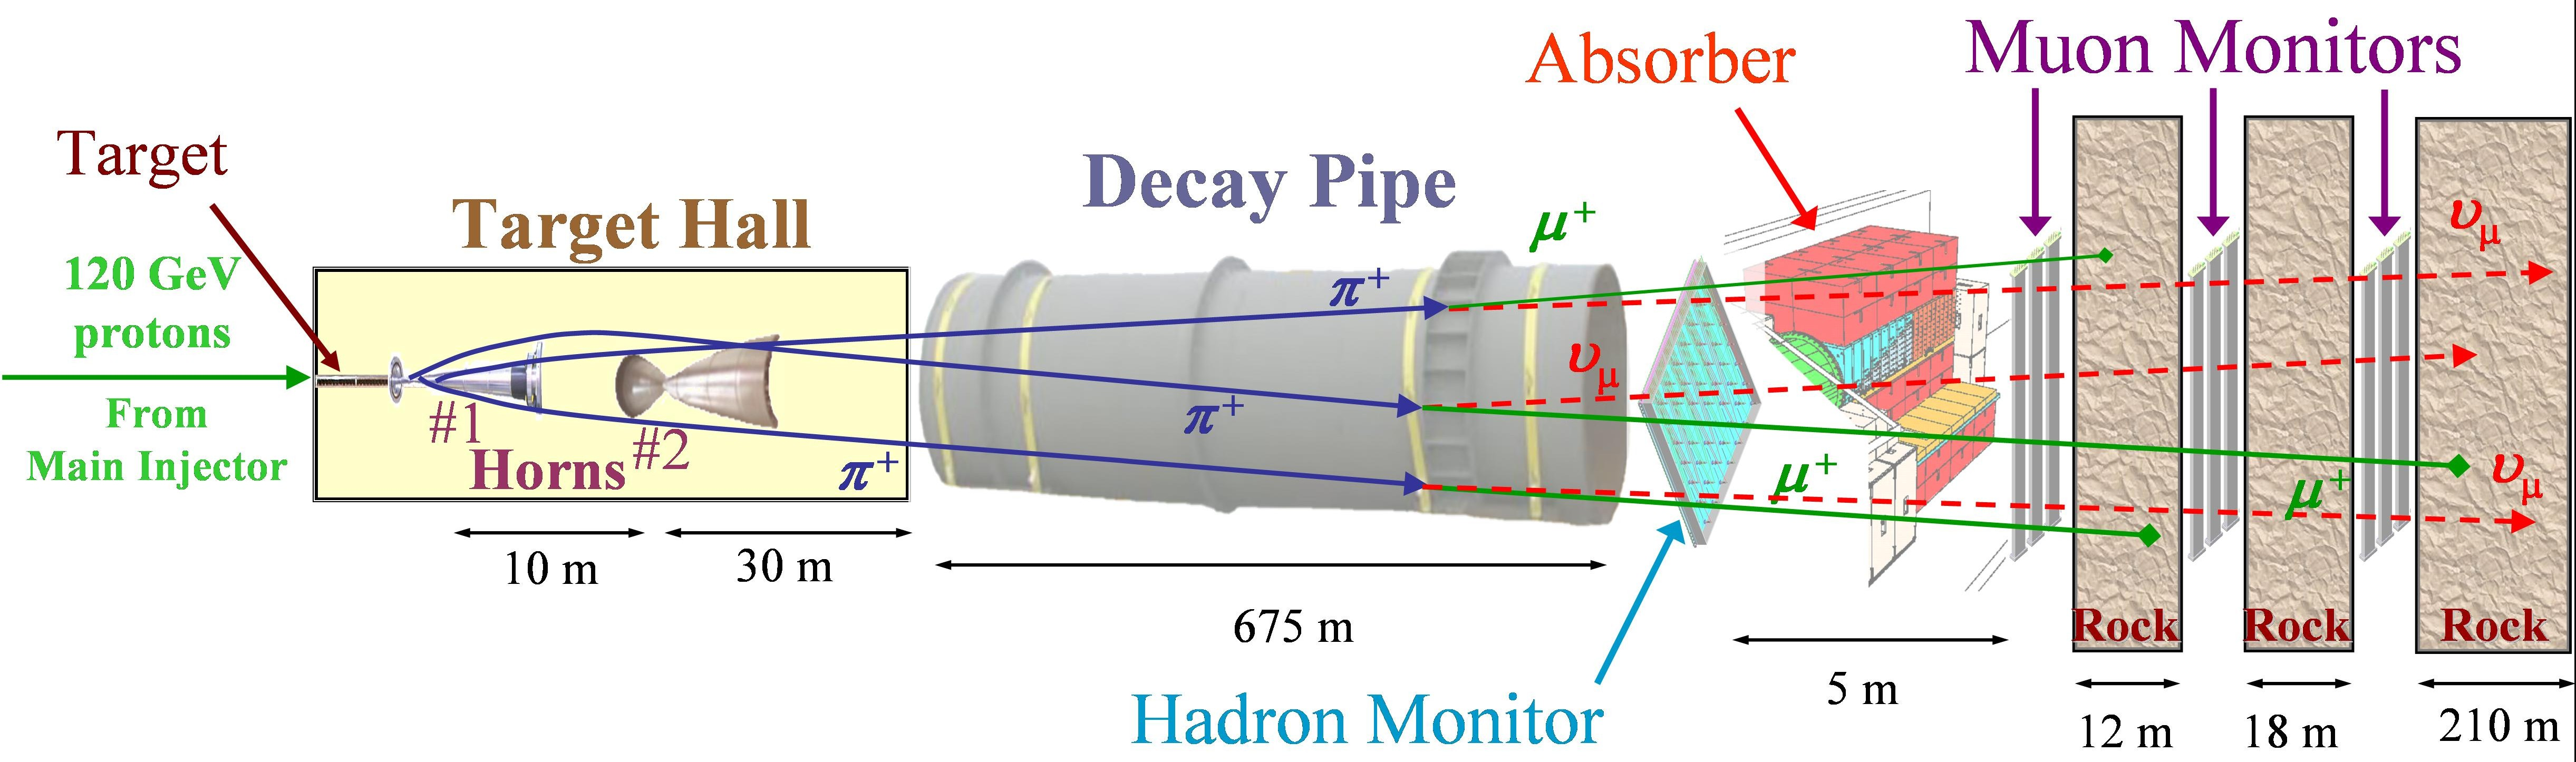
\includegraphics[width=\textwidth]{Plots/NOvAExperiment/BeamlineAlternative.jpg}
\caption[The schematic of the NuMI beam facility]{
The \acrshort{NuMI} neutrino beam starts on the left hand side with protons from the \acrshort{MI} impinged on a graphite target producing mainly pions and kaons. These are then focused and charge-selected by two focusing horns, after which they decay inside the decay pipe into a high-purity $\nu_\mu$ or $\overline{\nu}_\mu$ beam. The residual hadrons are stopped and monitored in the hadron absorber and the remaining muons are recorded with muon monitors and absorbed inside the rock. Figure from \cite{NuMI.pdf}.
%The schematic of the NuMI beam facility. The beam travels from left to right. The individual components shown are not to scale. Protons originate as $H^-$ ions, which are converted into protons in the Booster, sent to the main injector, where they are finally accelerated to $120\,\si{\giga\electronvolt}$, bent downward by $58\,\si{\milli\radian}$ and transported $350\,\si{\meter}$ to the $1.2\,\si{\meter}$ long NuMI target. The protons are incident on the graphite target and the produced hadrons are focused by two magnetic horns, located in about $40\,\si{\meter}$ long target hall, with about $19\,\si{\meter}$ separation between the two horns. Hadrons then enter a $675\,\si{\meter}$ long decay pipe made of steel, with $2\,\si{\meter}$ diameter, which serves as vacuum or low density environment for the mesons to propagate and decay into tertiary mesons, charged leptons and neutrinos. A hadron monitor is located at the end of the decay volume just in front of the $5\,\si{\meter}$ thick aluminium, steel and concrete absorber to record the profile of the residual hadrons. Of the particles interacting in the absorber, the principal component (approximately $80\%$) is the proton beam that has not interacted. The remainder are mainly mesons which have not decayed in the pipe or secondary protons. The absorber not only stops most of the particles still remaining in the beam but also acts as a shield against radiation. Muons and neutrinos deposit little or no energy in the absorber and continue into unexcavated rock with three muon monitors allowing measurement of the residual muon flux. The $240\,\si{\meter}$ of rock following the absorber stops the muons remaining in the beam but allows the neutrinos to pass\cite{numi}. 
}
\label{fig:NOvANuMI}
\end{figure}

The proton beam passes through a collimating baffle before hitting a $\sim\unit[1.2]{m}$-long (equal to about two interaction lengths) graphite target \cite{LEOFluxPredictionAtNuMI.pdf}, producing hadrons, predominantly pions and kaons \cite{NuMI.pdf}. These are then focused and selected by two parabolic magnetic `horns'. The focused hadrons pass through a $\unit[675]{m}$-long decay pipe filled with helium to create a low density environment for hadrons to propagate and decay in flight into either neutrinos or antineutrinos. High energy hadrons that do not decay in the decay pipe are absorbed within a massive aluminium, steel, and concrete hadron absorber and monitored with a hadron monitor. The leftover muons are ranged out in dolomite rock after the absorber and monitored using three muon monitors. The hadron and muon monitors are ionization chambers, used to monitor the quality, location and relative intensity of the beam.

Using a positive current inside the horns focuses positively charged particles, which then decay into neutrinos, and removes negatively charged particles. Reversing the horn current focuses negatively charged particles, which decay into antineutrinos, and defocuses positively charged particles. The neutrino mode is therefore called \gls{FHC} and the antineutrino mode is called \gls{RHC}. The composition of the neutrino beam for both these modes at the \gls{NOvA} \gls{ND} is shown in Fig.~\ref{fig:NOvABeamComponents}, displaying the very high purity of the $\nu_\mu$ or $\overline{\nu}_\mu$ component in the \gls{FHC} ro \gls{RHC} beam respectively \cite{NuMI.pdf}.

\begin{figure}[!htb]  
  \centering
  \includegraphics*[width=.495\textwidth]{Plots/NOvAExperiment/NuMIBeamComponentsNDFHC.pdf}
  \noindent\centering
  \includegraphics*[width=.495\textwidth]{Plots/NOvAExperiment/NuMIBeamComponentsNDRHC.pdf}
  \caption[NuMI neutrino beam components in the NOvA near detector]{The components of the neutrino beam at the \acrshort{NOvA} \acrshort{ND} per one \acrshort{NuMI} spill in the \acrshort{FHC} regime shown on the left and the \acrshort{RHC} regime on the right. The $\nu_\mu$ $\left(\overline{\nu}_\mu\right)$ composition in the \acrshort{FHC} (\acrshort{RHC}) regime is 93.8\% (92.5\%), with a wrong sign contribution of 5.3\% (6.6\%) and only 0.9\% (0.9\%) contamination by $\nu_e$ $\left(\overline{\nu}_e\right)$, showing the high purity of $\nu_\mu$ and $\overline{\nu}_\mu$ in the neutrino beam for \acrshort{NOvA}. Beam composition values calculated for neutrinos with energies between $\unit[1-5]{GeV}$. Figures are from internal \acrshort{NOvA} repository \cite{NOvA-doc-20843}.}
 \label{fig:NOvABeamComponents}
\end{figure}

The resulting neutrino beam energy distribution is peaked at $\sim\unit[7]{GeV}$ with a wide energy band. However, thanks to the kinematics of the dominant pion decay, by placing the \gls{NOvA} \gls{ND} and \gls{FD} $\unit[14.6]{mrad}$ ($\approx\unit[0.8]{\degree}$) off the main \gls{NuMI} beam axis, we achieve a narrow band neutrino flux peaked at $\unit[1.8]{GeV}$ \cite{NOvAResults2021.pdf,NOvATechreport.pdf}, as can be seen in Fig.~\ref{fig:NOvAOffAxis}. Using an off-axis neutrino flux increases the neutrino beam around $\unit[2]{GeV}$ about 5-fold compared to the on-axis flux and narrow-band peak enhances background rejection for the $\nu_e$ appearance analysis \cite{NOvATechreport.pdf}.

%Protons originate as $\textsc{H}^-$ ions, accelerated by the Linac to $\unit[400]{MeV}$, converted to protons and further accelerated to $\unit[8]{GeV}$ in the Booster, to be passed to the Main Injector which finally accelerates them to $\unit[120]{GeV}$ . Protons are then extracted, bent down to point towards the MINOS/NOvA Far Detector, and transported to the NuMI target \cite{NuMI.pdf}. The current beam power is $\sim\unit[700]{kW}$ with a plan \cite{PIP2.pdf} of reaching more than $\unit[1]{MW}$ beam power in the future upgrades.
%The NuMI target is a graphite fin, $\unit[7.4]{mm}$ wide, $\unit[63]{mm}$ tall and $\approx\unit[120]{cm}$ long (along the beam direction)\footnote{Previous target proportion were $\unit[6.4]{mm}$ W, $\unit[15]{mm}$ H and $\unit[95.38]{cm}$ L used in low energy design (see lower) \cite{NuMI.pdf}.} \cite{LEOFluxPredictionAtNuMI.pdf}. Protons interact in the target producing hadrons, predominantly pions and kaons \cite{NuMI.pdf}.

%The off-axis location means that both NOvA detectors are sited $14.6\,\si{\milli\radian}$ off the NuMI beam axis, in contrast to the MINOS Far Detector. This is because at around $14\,\si{\milli\radian}$, the energy of the neutrino does not have a strong dependence on the energy of the parent pion (fig. \ref{angleoff}), and also at this angle, the medium energy beam produces a narrow energy beam with approximately five times more neutrinos at $2\,\si{\giga\electronvolt}$ (fig. \ref{off-axis}), which is well-matched to the oscillation maximum expected to be at $1.6\,\si{\giga\electronvolt}$, thus maximizing the experiment’s neutrino oscillation sensitivity. In addition to the increased flux, the narrowness of the off-axis spectra enhances background rejection.\cite{techreport}

\begin{figure}[!htb]  
  \centering
  \includegraphics*[width=.48\textwidth]{Plots/NOvAExperiment/PionOffAxis.pdf}
  \noindent\centering
  \includegraphics*[width=.51\textwidth]{Plots/NOvAExperiment/OffAxisFluxPionEmbedded.pdf}
  \caption[The NOvA off-axis beam concept]{(Left) Dependence of the neutrino energy on the parent pion's energy and (right) neutrino energy distribution for an on-axis beam and three different off-axis beam designs. The case for \acrshort{NOvA} is shown in red and results in a narrow neutrino energy distribution around $\unit[2]{GeV}$, with limited dependence on the parent pion's energy. Figure from \cite{NOvATechreport.pdf}}
 \label{fig:NOvAOffAxis}
\end{figure}

\section{The NOvA Detectors}\label{sec:NOvADetectors}

The two main \gls{NOvA} detectors are the \gls{ND}, located in \gls{Fermilab} $\sim\unit[1]{km}$ from the \gls{NuMI} target and $\sim\unit[100]{m}$ under ground, and the \gls{FD}, located $\sim\unit[810]{km}$ from \gls{Fermilab} at Ash River in north Minnesota, partially underground with a rock overburden \cite{NOvATechreport.pdf}. \gls{NOvA} also operated a detector prototype called \gls{NDOS}, which was used for early research and development of detector components and analysis \cite{NOvAStatusAndOutlook.pdf}. Additionally, \gls{NOvA} operated a Test Beam detector, described in detail in Sec.~\ref{sec:TBDetector}. The scales of the \gls{ND} and \gls{FD} are shown in Fig.~\ref{fig:NOvADetectors}.

%The FD has an approximately 130kHz of cosmics

\begin{figure}[ht]
\centering
%is pdf-a
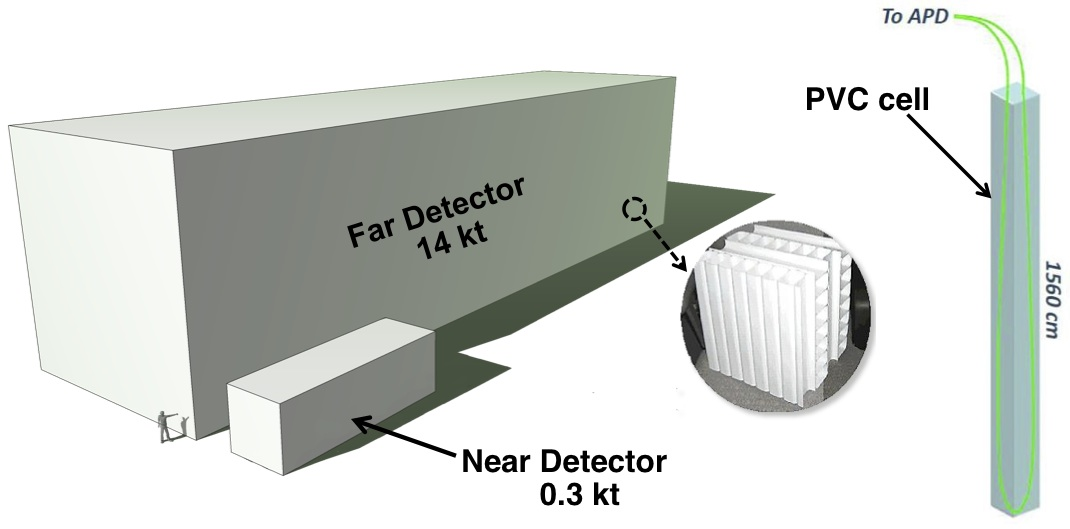
\includegraphics[width=1\textwidth]{Plots/NOvAExperiment/NOvADetectors.png}
\caption[NOvA detectors]{Schematic description of the scale and composition of the \acrshort{NOvA} \gls{ND} and \gls{FD}. The inset shows a photo of the orthogonal planes made out of \acrshort{PVC} cells. An example of a \acrshort{FD} cell containing liquid scintillator and a looped \acrshort{WLS} fibre attached to an \acrshort{APD} is shown on the right \cite{NeutrinoDetectorsForOscExp.pdf}.}
\label{fig:NOvADetectors}
\end{figure}

All \gls{NOvA} detectors are highly segmented, highly active, functionally identical tracking calorimeters made up of \gls{PVC} cells filled with liquid scintillator. Each cell is a long rectangular cuboid with depth of $\unit[5.9]{cm}$ and width of $\unit[3.8]{cm}$ (with some variations), with cell length extending to the full width/height of each detector, which is $\sim\unit[4.1]{m}$ for the \gls{ND} and $\sim\unit[15.6]{m}$ for the \gls{FD} \cite{NOvATechreport.pdf}. An example of a \gls{FD} cell is shown on the right of Fig.~\ref{fig:NOvADetectors}.

Cells are connected side-by-side into a 16 cell-wide extrusions with $\unit[3.3]{mm}$-wide walls between cells and $\unit[4.9]{mm}$-wide walls on the outsides of the extrusions. The first and last cell of each extrusion are $\sim\unit[3]{mm}$ narrower than the rest of the cells. Two extrusions are connected side-by-side to form a 32 cell-wide module, with each module having a separate readout (see Sec.~\ref{sec:DAQ}). In the \gls{FD}, 12 modules are connected side-by-side to form one plane of the detector. In the \gls{ND} only 3 modules make up a plane. Planes are positioned one after another, alternating between vertical and horizontal orientation, and grouped into diblocks, each containing 64 planes. The \gls{FD} contains 14 diblocks, totalling 896 planes, whereas the \gls{ND} contains 3 diblocks totalling 192 planes. The \gls{ND} also contains a Muon Catcher region, positioned right after the active region, consisting of 22 planes of the normal \gls{NOvA} detector design, 2 modules high and 3 modules wide, sandwiched with 10 steel plates to help range out muons mainly from the $\nu_\mu$ charged current interactions~\cite{NOvAStatusAndOutlook.pdf,NOvATechreport.pdf}.

The \gls{NOvA} coordinate system is centred with $\left(0,0,0\right)$ in the centre of the first plane, relative to the beam direction. The x axis runs from left to right when facing the detector, y axis from bottom to top and z axis runs perpendicular to the planes along the beam direction.

Each cell is filled with a liquid scintillator consisting of mineral oil with $4.1\%$ pseudocumene as the scintillant \cite{NOvAScintillators.pdf}. Each cell contains a single wavelength shifting fibre with double the length of the cell, looping at one end and connecting to the readout at the other. The \gls{PVC} walls of the cells are loaded with highly reflective titanium dioxide, with light typically bouncing off the \gls{PVC} walls $\sim8$ times before being captured by the \gls{WLS} fibre \cite{NOvATechreport.pdf}.
%As light travels through the fibre, it is attenuated by about a fraction of ten for the \gls{FD} cells \todo{Figure out what is the correct statement here}. 

The final dimensions of the \gls{FD} are $\unit[15.6]{m}\times\unit[15.6]{m}\times\unit[60]{m}$ with a total mass of $\unit[14]{kT}$ and for the \gls{ND} the dimensions are $\unit[3.8]{m}\times\unit[3.8]{m}\times\unit[12.8]{m}$ with a mass of about $\unit[0.3]{kT}$ \cite{NOvAHalfTimeOverview2022.pdf}. The active volume, consisting only of the liquid scintillator without the \gls{PVC} structure, makes up about $70\%$ of the total detector volume \cite{NOvATechreport.pdf}.

The \gls{NOvA} detectors are specifically designed for electromagnetic shower identification, with a radiation length of $\unit[38]{cm}$, which amounts to $\sim 7$ planes for particles travelling perpendicular to the detector planes \cite{NOvAStatusAndOutlook.pdf}. This is particularly useful to distinguish electrons from $\pi^0$s.

We can calculate the minimum energy an electron needs to have to cross one cell ($\unit[5.9]{cm}$) of the \gls{NOvA} detector by using the measured scintillator density $\unit[0.86]{g/cm^3}$ \cite{NOvA-doc-11886} and the electron range \cite{NISTParticleRangeTables} in the continuous slowing down approximation in a Polyethylene (approximation of the \gls{NOvA} scintillator \cite{NOvA-doc-13579-FACalorimetricEnergyScale}), as $E_{e}\gtrsim\unit[15]{MeV}$.
%We can calculate what is the minimum energy for any particle to be recorded in the \gls{NOvA} detector, by taking the density of \gls{NOvA} liquid scintillator as $\unit[0.86]{g/cm^3}$ \cite{NOvA-doc-11886} and looking up the particle range in the continuous slowing down approximation and approximating the liquid scintillator as polyethylene \cite{NOvA-doc-13579-FACalorimetricEnergyScale}. We take the depth of one \gls{NOvA} cell ($\unit[5.9]{cm}$) as the minimum distance particle needs to travel to be recorded in the \gls{NOvA} detector. For electrons we get that the minimum energy an electron needs to have to be recorded in \gls{NOvA} is $\sim\unit[15]{MeV}$ \cite{NISTParticleRangeTables}. 
%The MIP energy loss for electrons (similarly to muons) can be found with a similar method as used in the AbsCal\_technote\_1stAna in TestBeam (page 2)

\section{Readout and Data Acquisition}\label{sec:DAQ}

The signal from the \gls{WLS} fibres is read out by an \gls{APD}, converting the scintillation light into electrical signal, with a high quantum efficiency of $\sim 85\%$ and a gain of $100$ \cite{NOvATechreport.pdf}. An example \gls{APD} is shown in Fig.~\ref{fig:NOvAAPD}. Both ends of each fibre are connected to one of the 32 pixels on the \gls{APD}, with each \gls{APD} reading out signal from one module. To maximise the signal to noise ratio, the \gls{APD}s are cooled to $\unit[-15]{\degree C}$ by a thermoelectric cooler, with heat carried away by a water cooling system.

The combination of the \gls{APD} quantum efficiency and the light yield, determined by the \gls{PVC} reflectivity and the scintillator's and \gls{WLS} fibre's response, result in a signal requirement of at least 20 photoelectrons in response to minimum ionizing radiation at the far end of the \gls{FD} cell.

%TDR-12.2.1:"NOvA readout electronics requires, at minimum, a 20 photoelectron signal in response to minimum ionizing radiation at the far-end of a 15.5 m NOvA cell as discussed in Chapter 6. The signal strength is due to the APD quantum efficiency and the light yield in response to ionizing radiation. The light yield, in turn, is due to a combination of the PVC reflectivity, the scintillator and wavelength-shifting fiber responses."

%For some reason the TDR I have downloaded doesn't have the full chapter 14. Full TDR can be found in docdb:2678 chapter by chapter.

\begin{figure}[!htb]  
  \centering
  \includegraphics*[width=.495\textwidth]{Plots/NOvAExperiment/NOvAAPDMountedWithLabels.jpg}
  \noindent\centering
  \includegraphics*[width=.495\textwidth]{Plots/NOvAExperiment/NOvAAPDBottomWithLabels.jpg}
  \caption[NOvA Avalanche Photo Diods]{The modules with \acrshort{APD}s for \acrshort{NOvA} mounted on top of the detector on the left picture, and shown from the bottom on the right. The individual components of the module are described. The left picture shows a disconnected ribbon cable and ground cable, which are normally connected to the front end board.}
 \label{fig:NOvAAPD}
\end{figure}

Each \gls{APD} is connected to a single \gls{FEB}, shown in Fig.~\ref{fig:NOvAFEB}. The \gls{FEB} amplifies and integrates the \gls{APD} signal, determines its amplitude and arrival time, before passing it to the \gls{DAQ} system. On the \gls{FEB} the \gls{APD} signal is first passed to a custom \gls{NOvA} \gls{ASIC}, which is design to maximize the detector sensitivity to small signals. \gls{ASIC}s amplify, shape and combine the signal, before sending it to an \gls{ADC}. The combined noise from the \gls{APD} and the amplifier is equivalent to about 4 \gls{PE}s, which, compared to an average photoelectron yield from the far end of the \gls{FD} cell of 30, results in a good signal and noise separation \cite{NOvATechreport.pdf}. The digitized data from an \gls{ADC} is sent to a \gls{FPGA}, which extracts the time and amplitude of the \gls{ADC} signals, while subtracting noise based on a settable threshold. The \gls{FPGA}s employ multiple correlated sampling methods to reduce noise and improve time resolution of the signal \cite{NOvADAQ.pdf}.

\todo{Find out what is the pedestal/threshold that's being subtracted}

\begin{figure}[!htb]  
  \centering
  \includegraphics*[width=\textwidth]{Plots/NOvAExperiment/NOvAFEBWithLabels.jpg}
  \caption[NOvA Front End Board]{An example of a \acrshort{NOvA} \acrshort{FEB} with individual components labelled.}
 \label{fig:NOvAFEB}
\end{figure}

%TDR:Major components are the carrier board connector location at the left, which brings the APD signals to the NOvA ASIC, which performs integration, shaping, and multiplexing. The chip immediately to the right is the ADC to digitize the signals, and FPGA for control, signal processing, and communication. Data from the ADC is sent to an FPGA where multiple correlated sampling is used to remove low frequency noise. This type of Digital Signal Processing (DSP) also reduces the noise level and increases the time resolution.

All of the \gls{NOvA} front end electronics (\gls{APD}s and \gls{FEB}s) are operated in a continuous readout mode, without requiring any external triggers \cite{NOvATechreport.pdf}. Due to higher detector activity during beam spills, the \gls{ND} \gls{FEB}s work at a higher frequency of $\unit[8]{MHz}$, whereas the \gls{FD} \gls{FEB}s suffice with $\unit[2]{MHz}$ sampling frequency \cite{NOvADAQ.pdf}.

Data from up to 64 \gls{FEB}s are concentrated in a \gls{DCM}, which concatenates and packages the data into $\unit[5]{ms}$ time slices, before sending it to the buffer nodes. \gls{DCM}s are also connected to the timing system and pass a single unified timing measurement to the \gls{FEB}s to maintain synchronization across the detector~\cite{NOvADAQ.pdf}.
%The timing information is calibration off-line to account for differences between fibre and cable distances and to achieve a superb timing resolution \cite{NinerThesis} - I don't think I need to talk about the timing calibration here tbh. The NOvA calibration process technically also involves \textbf{timing calibration}, which corrects for the time differences of the signal to be processed \cite{NinerThesis}.

The buffer nodes cache the data for at least 20 seconds while receiving information from the trigger system. Each trigger uses a time window based either on the time of the \gls{NuMI} beam spill, on a periodic interval for readout of comic events for detector calibration and monitoring, or on a time of activity-based data-driven trigger \cite{NOvADAQ.pdf}. Data that fall within any of the trigger windows are sent to a data logger system, where they are merged to form events, before being written to files for offline processing, or sent to an online monitoring system.

%Data for calibration and non-beam physics channels is collected and a variety of data-driven triggers using real-time reconstruction algorithms run on data stored in an online buffer farm at each detector [26].  Beam events are collected in both detectors using a 550 μs time window centered on the 10 μs beam spill window, triggered by a signal derived from the accelerator controls system. The wide time window of data collection compared to the beam spill is used to sample cosmic-ray activity and noise under the precise detector conditions that apply to the beam data. [NOvAHalfTimeOverview2022.pdf]

%Maybe I should write here what is the event rate?

%Maybe write about what information do we have about each event at this stage: timing, peak ADC, cell, plane, run, subrun. Grouped into triggered windows?
% "the time, location, and pulseheight of those signals are recorded as a hit" [NOvAHalfTimeOverview2022.pdf]

\todo{Talk about data quality as well, since I talk about good runs and bad channels in the TB calib chapter}

\section{Simulation}\label{sec:NOvASimulation}

\note{Should I divide the simulation into the individual stages? I had it like that originally, but for example the simulation of cosmics is only very short and not sure what section would I put it under}

To extract neutrino oscillation parameters, or to test a hypothesis, \gls{NOvA} uses a series of simulations to make predictions according to various physical models \cite{NOvASimulationOld-Fluka.pdf}.
%To simulation the expected signal from the NOvA detectors,
%To get a prediction of any possible signal events or their background in the NOvA detectors,
% we use a series of simulations, tuned or corrected by both internal and external measurements to better match the current state of the art knowledge \cite{NOvASimulationOld-Fluka.pdf}.
The simulation chain can be divided into four parts: simulation of the neutrino beam, simulation of neutrino interactions within the \gls{NOvA} detectors, simulation of cosmic particles interacting in the \gls{NOvA} detector and simulation of the detector response.

To simulate the neutrino beam, \gls{NOvA} uses the \texttt{GEANT4} v9.2.p03~\cite{GEANT4.pdf} based \gls{MC} simulation with a detailed model of the \gls{NuMI} beamline \cite{ZPavlovicThesisG4NuMI_2008.pdf}, as it was described in Sec.~\ref{sec:NOvASimulation}. The simulation starts with \gls{MI} protons interacting within the long carbon target and producing hadrons, mainly $\pi, K$ and $p$, followed by transport and possible further interaction of these hadrons within the focusing system, until finally ending with hadron decays producing the neutrino beam.

To account for the imprecise theoretical models used in GEANT4, we use the \gls{PPFX} to incorporate external measurements of yields and cross sections of hadron production inside the target and other \gls{NuMI} materials into the prediction~\cite{NuMIFlux.pdf}. The current version of \gls{PPFX} is limited by the results available during its creation and only corrects the most frequent interactions while assigning large systematics uncertainties to the rest (see Sec.~\ref{sec:NOvASystematics}). For the most common $\pi$ production, \gls{PPFX} uses the NA49 measurements \cite{NA49:Inclusive_production_of_charged_pions.pdf} of $\unit[158]{GeV/c}$ protons interacting on a thin (few percent of interaction length) carbon target, with a few data point from Barton et al~\cite{BartonHadProd1983.pdf} to expand the kinematic coverage. These then have to be scaled to the $\unit[20-120]{GeV/c}$ incident proton energies seen in \gls{NOvA} using the FLUKA \cite{FLUKA_01,FLUKA_02} \gls{MC} generator. For the $K$ production from $p+C$ interaction, important for higher neutrino energies and electron neutrinos, \gls{PPFX} uses the NA49 $K$ data \cite{NA49DataKaons.pdf} together with the NA49 $\pi$ data \cite{NA49:Inclusive_production_of_charged_pions.pdf} multiplied by the $K/\pi$ ratios of yields on thin carbon target from the MIPP experiment \cite{pionToKaonIn_pC.pdf}. Lastly, for the nucleon production, \gls{PPFX} uses the NA49 data on quasi elastic interactions \cite{NA49pc-proton2013.pdf}. All the other interactions inside \gls{NuMI}, such as interaction in non-carbon targets, or interactions with hadrons other than protons, are either extrapolated from the previously mentioned measurements, or are not corrected for and a significant systematic uncertainty is assigned to them \cite{NuMIFlux.pdf}.

There's two new experiments that measured the production and interaction of hadrons on various targets and incident energies, specifically designed to improve the prediction of neutrino beams. I worked on implementing data from the NA61 experiment on hadron production from $p+C$ interaction on a thin carbon target at $\unit[31]{GeV/c}$~\cite{2015_hadron_prod_pC_2009data.pdf}, motivated by possible reduction in the $K$ production systematic uncertainty. This work is still ongoing and will be implemented into \gls{PPFX} and \gls{NOvA} together with the rest of the NA61 measurement. The most impactful ones will be the measurement of hadron production from $p+C$ interaction on a thin carbon target at $\unit[120]{GeV/c}$ \cite{NA61_hadprodFrompC_120GeV_2023.pdf} (no energy scaling required), measurements of $p+C$ and $p+Be$ at different incident energies \cite{2019_NA61_ProdAndInelXSec_protonOnDiffTargets60And120GeV._results.pdf}, $\pi+C$ and $\pi+Be$ measurements at $\unit[60]{GeV/c}$~\cite{2019_had_prod_at_Pi_on_C_and_Be.pdf}, resonance production measurements from $\unit[120]{GeV/C}$ $p+C$ \cite{NA61_ResonanceProdFrompC_120GeV_2023.pdf}, and probably the most impactful one, the yet unpublished measurement of hadron production yield on a \gls{NOvA}-era \gls{NuMI} replica target at $\unit[120]{GeV/c}$ \cite{ThickTargetLimit.pdf}. NA61 also measured the hadron production yield for the \gls{T2K} experiment's replica target \cite{2019_hadron_yields_T2K_replica.pdf}, which significantly reduced the neutrino flux systematic uncertainty for the \gls{T2K} measurements \cite{ThickTargetLimit.pdf}. The second experiment is EMPHATIC~\cite{EMPHATICProposal2019.pdf}, which is currently analysing their data on a broad range of hadron production measurements, mainly the secondary and tertiary interactions of various projectiles with a wide range of incident energies and thin target materials, complementary to the NA61 measurements.

%From NOvAResults2021.pdf: The neutrino flux delivered to the detectors is calculated using GEANT4-based simulations of particle production and transport through the beamline components [NuMI.pdf,GEANT4.pdf] reweighted to incorporate external measurements using the package to predict the flux (PPFX) [NuMIFlux.pdf,30–48].

%From NOvAResultsCombinedNuAnu2019.pdf: The flux of neutrinos delivered to the detectors is calculated using a simulation of the production and transport of particles through the beamline components [22,25] reweighted to incorporate external measurements [26–45].

%From NOvAHalfTimeOverview2022.pdf: Neutrino interactions in NOvA are simulated with a chain of software packages. The neutrino flux is modeled using G4NuMI, a geant based description of the NuMI beam line [Z. Pavlovic thesis]. The raw flux from G4NuMI is then modified using the PPFX package to better match the products of the interactions in the extended target to the world’s hadron production data [NuMIFlux.pdf].

%%%%%%%%%%%%%%%%%%%%%%%%%%%%%%%%%%%%%%%%%%%%%%%%%%%%%%%%%%%%%%%%%%%%%%%%%%%%%%%
%%%% Master's thesis on flux simulation
\iffalse
There are often multiple interactions within the target and in the materials downstream of it and since the hadron production process is governed by non-perturbative QCD and occurs in the nucleus, highly accurate theoretical predictions are not possible \cite{NuMIFlux.pdf,LEOFluxPredictionAtNuMI.pdf}. NOvA therefore tunes and corrects possible mismodeling of the model using external data in a package developed for MINERvA experiment called Package to Predict the Flux (PPFX) \cite{LEOFluxPredictionAtNuMI.pdf}.

%...Those models are not necessarily accurate but can be tuned or benchmarked by comparing their predictions to measurements of hadron production. Recent measurements of pion production on a thick (two interaction length) carbon target have been released by MIPP [4], and measurements of pion production on a thin (few per cent interaction length) carbon target are available from NA49 [5]. In addition, there are several other hadron production measurements on various materials, using both proton and pion beams, that can be used to constrain a neutrino beamline simulation.[NuMIFlux.pdf]

%Roughly 85% of the interactions that produce particles that lead to muon neutrinos passing through MINERvA are from protons interacting on carbon. Other relevant materials are aluminum (horns), iron (decay pipe walls), helium (decay pipe gas), and air (target hall). Interactions of π ± , K ± and n created in the initial proton interaction, or subsequent interactions, are subdominant but non-negligible. When protons collide with carbon, the interactions can produce pions, kaons, neutrons, strange baryons, and lower energy protons. These particles, if they do not decay first, can interact either in the target or in other downstream material to create tertiary particles that can also decay into neutrinos. \cite{NuMIFlux.pdf}

PPFX is used to correct each interaction of neutrino's ancestry chain by weighting it with a factor computed from external experimental measurements of yields or invariant differential cross-sections \cite{LEOFluxPredictionAtNuMI.pdf}

The kinematic values of the initial particles (like the initial $\unit[120]{GeV}$ proton interacting on carbon in NuMI) are not always the same between the measured interaction and the required values. To solve this we use the \textit{Feynman-x} ($x_{F}$) scaling variable. Feynman speculated \cite{feynman1969.pdf} that expressing the cross-sections of inclusive high energy hadronic collisions in terms of $x_{F}$ would make the cross-section scaling energy independent \cite{LEOFluxPredictionAtNuMI.pdf}.
%$c_i$ is the \textit{central value} of the weight

There are two main experiments whose results are used in the PPFX. NA49 \cite{NA49:Inclusive_production_of_charged_pions.pdf}, which used $\unit[158]{GeV}$ protons interacting on carbon thin target, and MIPP \cite{pionToKaonIn_pC.pdf} which used protons from the Main Injector and both thin carbon target and the low energy NuMI target (thick target) \cite{PPFXTechnote2017.pdf}. Energy scaling of the external data to calculate the PPFX weight is performed by FLUKA\cite{NuMIFlux.pdf}

%%% Hadron production datasets:
%There are two major datasets available to constrain the process where protons interact on carbon and produce charged pions. One measurement, from NA49 [5], uses a thin target with an incident proton momentum of 158 GeV/c. The other measurement, from MIPP [4], uses an actual NuMI LE target and 120 GeV/c protons. These two datasets will be used to make separate “thin target” and “thick target” flux predictions by weighting each interaction leading to a neutrino going through MINERvA. We also use additional datasets to constrain kaon and nucleon production, and the absorption of particles in beamline materials. Where multiple interactions are constrained with data, the overall weight applied to the neutrino event is simply the product of the weights for each interaction.\cite{NuMIFlux.pdf}

For kaons with $x_{F}<0.2$ PPFX uses weights based on NA49 measurements\cite{NA49DataKaons.pdf} and for kaons with $0.2<x_{F}<0.5$ PPFX uses the $K/\pi$ yield ratio from the MIPP thin target measurements\cite{pionToKaonIn_pC.pdf} multiplied by NA49 thin target yields.
\fi
%%% End of master's on flux simulation
%%%%%%%%%%%%%%%%%%%%%%%%%%%%%%%%%%%%%%%%%%%%%%%%%%%%%%%%%%%%%%%%%%%%%%%%%%%%%%%

%Good description of PPFX, beam transport and the principal components is in the NOvA-T2K technote for Flux (doc-db:54582) https://nova-docdb.fnal.gov/cgi-bin/sso/ShowDocument?docid=54582

\note{The description of neutrino interactions, including QE/Res/DIS scattering and nuclear effects will probably be in the theory chapter. If not I'll add it here.}
\note{Might have to describe some of these interaction models a bit more if any of the cross section uncertainty for the magnetic moment analysis turns up to be significant}

The output of the neutrino beam simulation is passed to the simulation of neutrino interactions inside the detectors, which is done with the GENIE v3.0.6~\cite{GENIE.pdf} neutrino \gls{MC} generator. GENIE allows users to choose the particular models for different types of neutrino interactions and particle propagation within the nucleus, as well as possible tunes to external measurements. The four main interaction modes in GENIE are the \gls{QE} \gls{CC} scattering, the \gls{Res}, the \gls{DIS}, and the \gls{COHpi}. Special case of \gls{CC} interaction with two nucleons producing two holes via \gls{MEC} is also considered. Particles created in these processes are then propagated inside the nucleus according to the \gls{FSI}. All of these are set by the \gls{CMC} and \gls{NOvA} currently uses the \texttt{N1810j0000} \gls{CMC}. Additionally, \gls{NOvA} adds a tune to \gls{NOvA} $\nu_\mu$\gls{CC} data for the \gls{CC}\gls{MEC} interactions and a set of external $\pi$ interaction measurements to constrain the \gls{FSI} model. Table~\ref{tab:NuIntSimulationModels} shows the list of models and tunes for different interaction modes in \gls{NOvA} \cite{NOvAResults2021.pdf}. \todo{Also describe the nuclear models}

\begin{table}[!ht]
\centering
%\def\arraystretch{1.4}
\caption{Models and tunes used in the NOvA simulation of neutrino interactions.}
\begin{tabular}{|l|l|l|}
\hline
Interaction & Model                  & Tune\\\hline
\gls{CC}\gls{QE} & Val\`{e}ncia \cite{ValenciaModel_NOvACCQE_2004.pdf} & External $\nu-\textsf{D}$ data \cite{NuDeuteriumScattering_NOvACCQETune_2016.pdf}\\
\gls{CC}\gls{MEC} & Val\`{e}ncia \cite{ValenciaModel_NOvACCQEMEC_2011.pdf,ValenciaModel_NOvAMEC_2013.pdf} & \gls{NOvA} $\nu_\mu$\gls{CC} data\\
\gls{Res} \& \gls{COHpi} & Berger-Sehgal \cite{BergerSehgal_ResonancePionProd_2007.pdf,BergerSehgalModel_CohPionProd_2009.pdf}          & External $\nu-A$ data\\
\gls{DIS} & Bodek-Yang \cite{BodekYangModel_NOvADIS_2003.pdf,HadronizationModelForNuDIS_NOvADIS_1988.pdf}            & External $\nu-A$ data\\
\gls{FSI} & Semi-classical cascade \cite{FSIModel_hNSemiClassicalCascade_1988.pdf} & External $\pi-^{12}\textsf{C}$ data\\\hline
\end{tabular}
\label{tab:NuIntSimulationModels}
\end{table}

%NOvANuMuCCPi0XSecMeasurement2023.pdf: Neutrino interactions are simulated with GENIE [17] v2.10.2. The GENIE simulation generates interactions via its four default production processes: quasielastic scattering, resonant baryon production, deep-inelastic scattering, and coherent pion production. Particles created via these primary processes are subsequently propagated though the nuclear medium using GENIE’s hA effective cascade FSI model [18,19].

% Describe that GENIE is highly costumizable and you can set up any generators you like. Ideally describe what parts are purely theoretical and what parts are tuned to external data. Also mention that NOvA is doing an internal tune to some of the parameters.

%From NOvAResults2021.pdf: Neutrino interactions are simulated using a custom model configuration of GENIE 3.0.6 [49,50] tuned to external and NOvA ND data.
%In this configuration, charged-current (CC) quasielastic (QE) scattering is simulated using the model of Nieves et al. [53], which includes the effects of long-range nucleon correlations calculated according to the random phase approximation (RPA) [53–55]. The CCQE axial vector form factor is a z-expansion parametrization tuned to neutrino-deuterium scattering data [56].
%CC interactions with two nucleons producing two holes (2p2h) are given by the IFIC València model [57,58]. The initial nuclear state is represented by a local Fermi gas in both the QE and 2p2h models, and by a global relativistic Fermi gas for all other processes.
%Baryon resonance (RES) and coherent pion production are simulated using the Berger-Sehgal models with final-state mass effects taken into account [59,60].
%Deep inelastic scattering (DIS) and nonresonant background below the DIS region are described using the Bodek-Yang model [61] with hadronization simulated by a data-driven parameterization [62] coupled to PYTHIA [63].
%Bare nucleon cross sections for RES, DIS, and nonresonant background processes are tuned by GENIE to neutrino scattering data.
%Final-state interactions (FSI) are simulated by the GENIE hN semi-classical intranuclear cascade model in which pion interaction probabilities are assigned according to Oset et al. [64] and pion-nucleon scattering data.

%The 2p2h and FSI models in this GENIE configuration are adjusted to produce a NOvA-specific neutrino interaction model tune. The 2p2h model is fit to $\nu_\mu$CC inclusive scattering data from the NOvA ND. Inspired by Gran et al. [65], this 2p2h tune enhances the base model as a function of energy and momentum transfer to the nucleus and is applied to all CC 2p2h interactions for both the neutrino and antineutrino beams. 
%The parameters governing $\pi^\pm$ and $\pi^0$ FSI are adjusted to obtain agreement with $\pi^+$ on $^{12}\textsf{C}$ scattering data [66–72].

%From NOvAResultsCombinedNuAnu2019.pdf: Neutrino interactions in the detector are simulated using GENIE [46] tuned to improve agreement with external measurements and ND data, reducing uncertainties in the extrapolation of measurements in the ND to the FD. As in Ref. [21], we set MA in the quasielastic dipole form factor to 1.04 GeV/c2 [47] and use corrections to the charged-current (CC) quasielastic cross section derived from the random phase approximation [48,49]. In this analysis, we also apply this effect to baryon resonances as a placeholder for the unknown nuclear effect that suppresses rates at a low four-momentum transfer in our and other measurements [50–53]. Additionally, we increase the rate of deep-inelastic scattering with hadronic mass W > 1.7 GeV/c2 by 10\% to match our observed counts of short track-length $\nu_\mu$CC events. We model multinucleon ejection interactions following Ref. [54] and adjust the rates in bins of energy transfer, $q_0$, and three-momentum transfer, $\left|\overrightarrow{q}\right|$, for $\nu_\mu$ and $\overline{\nu}_\mu$ separately to maximize agreement in the ND. The calculation of the $\nu_e$ and $\overline{\nu}_e$ rates uses these same models.

%From NOvAHalfTimeOverview2022.pdf: Neutrino interactions and final state interactions are modeled using the GENIE neutrino interaction generator [31]

%From master thesis: From there GENIE event generator \cite{GENIE.pdf} simulates neutrino interactions in the detector \cite{2019NOvAFHCRHCResults.pdf} and another GEANT4 simulates the detector response \cite{NOvASimulationOld-Fluka.pdf}. NOvA also tunes the cross-section model of the GENIE simulation to the ND data to reduce uncertainties in the extrapolation of measurements on the ND to the FD \cite{2019NOvAFHCRHCResults.pdf}.

Since the \gls{FD} is on the surface we also need to include a simulation of cosmic rays generated with the \gls{CRY} \cite{CRY} \gls{MC} generator. The simulated cosmic muons are also used to calibrate \gls{NOvA} detectors \cite{NuMIFlux.pdf}. 

Particles that are created from neutrino interactions and cosmic rays are propagated through the \gls{NOvA} detectors using an updated version of \texttt{GEANT4} v10.4.p02~\cite{GEANT4.pdf}. The output of this simulation is the energy deposited in the scintillator, which is then passed to a custom \gls{NOvA} simulation software \cite{NuMIFlux.pdf}. The scintillation light generated by the deposited energy is parametrized using the Birks-Chou model \cite{BirksChouParametrization_1952.pdf}, which corrects for recombination in organic scintillators at high deposited energies. The normalization factors for the produced scintillation light (the light yield), as well as for the Cherenkov light, which can affect the light readout, are tuned to \gls{NOvA} cosmic data~\cite{NOvANumuCCXSexMeasurement2023.pdf}. The light collection by the \gls{WLS} fibres and its transport to the \gls{APD}s, as well as the \gls{APD} response use a parametrized simulation, which makes use of the fact that all the \gls{NOvA} cells and their readout are generally the same across the detectors \cite{NuMIFlux.pdf}. The simulation of the readout electronics is done by another custom \gls{NOvA} parametrized model, which mainly account for a random electronics noise, with output in the same format as raw data.

%NuMIFlux.pdf: While GEANT4 is capable of simulating optical photon processes, generating scintillation light and propagating it through the cell, up the fiber, and to the APD is very time consuming. Instead, we observe that the NOvA detectors are composed of many identical readout cells as shown in Fig. 6, so if we can generate templates to parameterize photon transport once, we can use them everywhere. The processes we must be able to parameterize are: the collection of scintillation photons by the fiber, the transport of light up the fiber, and the response of the APD to the captured light.

Due to the high neutrino rate in the \gls{ND}, there are neutrinos interacting in the surrounding rock creating particles that make it to the detector and act as background. To simulate these rock events we use the same simulation as for neutrino interactions inside the detector. However, since only a few particles make it into the detector, it would be very time consuming to run this simulation for every neutrino. Therefore, we create a separate simulation that includes the surrounding rock and then overlay the results into the normal \gls{NOvA} simulation chain, which doesn't include the rock, so that the rate matches the \gls{NuMI} neutrino rate \cite{NuMIFlux.pdf}.

%%% Rock simulation and overlay
%NuMIFlux.pdf: Due to the high beam intensity at the near detector, many neutrinos interact in the rock in front of the detector. Simulating these interactions requires allowing GEANT4 to propagate muons through a very large rock volume which is a slow process, and only a few of these muons will make it into our detector. To correctly account for this, we simulate many neutrino interactions with the mother volume including a large rock volume in front of the detector, and only keep those that leave energy in the detector. During normal simulation, with the mother volume only including the detector and the immediate detector hall, we overlay these rock ’singles’ at a rate determined during the generation of flux files after the GEANT4 stage.

\section{Data Processing and Event Reconstruction}\label{sec:NOvAReconstruction}
Both data and simulation events for all \gls{NOvA} detectors are passed through the same event reconstruction and particle identification algorithms. The reconstruction was specifically developed with the $\nu_e$ appearance search in mind, focusing on identifying the $\nu_e$\gls{CC} signal against the $\nu_\mu$\gls{CC} and \gls{NC} backgrounds. Each \gls{NOvA} detector has to deal with a different challenges, with multiple neutrinos interacting in the \gls{ND} during one beam spill, and a large cosmic background in the \gls{FD} \cite{NOvAReco.pdf}.

The readout from each cell from the \gls{DAQ} (see Sec.~\ref{sec:DAQ}) is called a \textit{channel} and the \gls{DAQ} output from each channel is called a \textit{raw hit}. \gls{DAQ} groups hits into $\unit[550]{\mu s}$ windows and passes them to an offline reconstruction chain~\cite{NOvAReco.pdf}. Reconstruction starts by grouping hits into \textit{slices} based on their proximity to other hits in both time and space~\cite{DBSCAN.pdf}.
\note{Maybe include rawhit to cellhit to recohit}
%[RelCal_technote_1stAna.pdf] CalHit transforms RawDigits into CellHits. This is a transformation of the channel numbering system to offline (plane/cell) coordinates, and the fine-timing fit. A RecoHit can by created from a CellHit by passing it and an estimated W position to Calibrator, or by asking one of the RecoBase objects, which calculate best-guess W positions for their constituent cells.

For events that produce hadronic and electromagnetic showers, we first identify lines through major features using a modified Hough transform~\cite{HoughTransform.pdf}. These lines representing momentum directions are then passed to the Elastic Arms algorithm~\cite{ElasticArms.pdf} to identify \textit{vertex} candidates from their intersection points. Hits are then clustered into \textit{prongs}, group of hits with a start point and a direction, using a k-means algorithm called FuzzyK \cite{FuzzyKClustering.pdf,FuzzyKFuzzyness.pdf}. Here `fuzzy' means that each hit can belong to multiple prongs. Prongs are first created separately for each view (also called 2D prongs) and then, if possible, view-matched into 3D prongs (or just prongs)~\cite{NOvAReco.pdf}. Figure~\ref{fig:NOvARecoEVD} shows an example simulated electron shower with the reconstructed vertex (red cross) and prong (red shaded area) grouping all hits that should be a part of the shower together, while removing background hits in grey.\todo{Describe the Cosmic Ray Vertex used for data-based simulation}

\begin{figure}[ht]
\centering
%is pdf-a
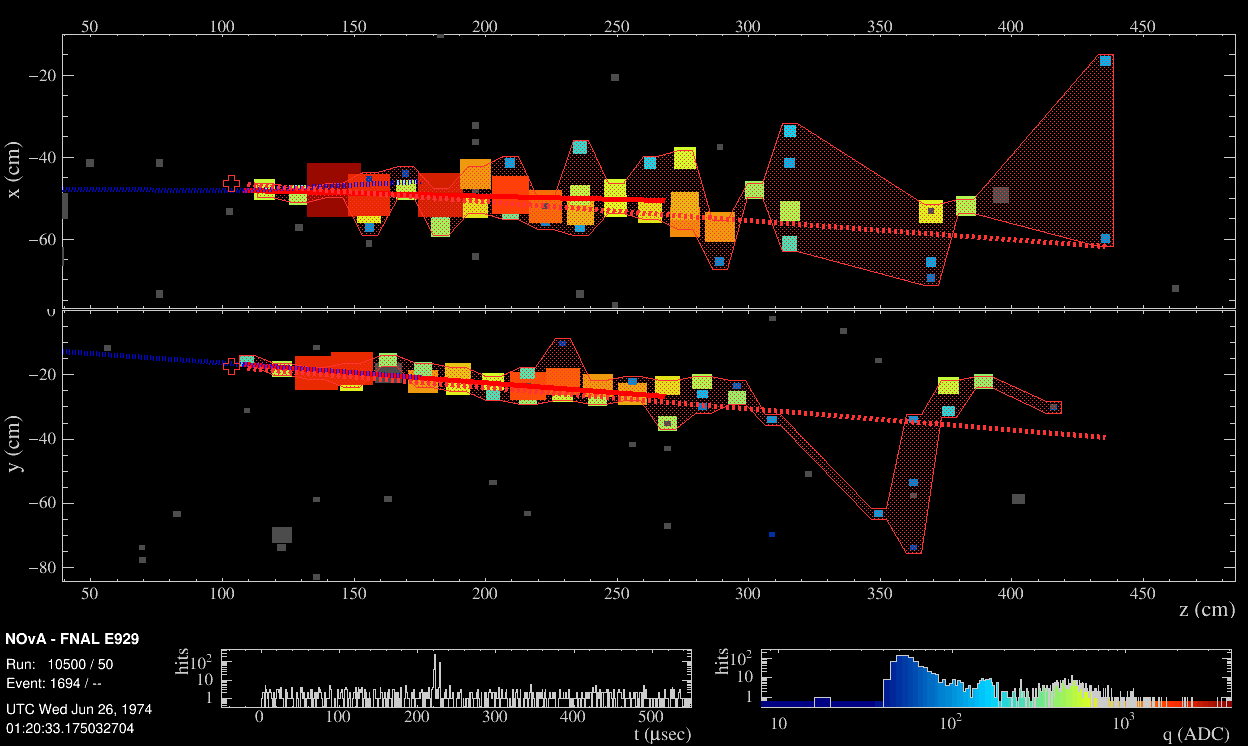
\includegraphics[width=1\textwidth]{/home/robert/Documents/School/PhD/Thesis/Plots/NOvAExperiment/ElectronRecoEVD.png}
\caption[NOvA reconstruction of a single electron]{Reconstruction of a simulated single electron event in the \acrshort{NOvA} \acrshort{ND}. The red cross is the reconstructed vertex, the shaded area shows the cluster of hits into a shower and the dotted red line shows the estimated momentum of that shower. The blue dotted line shows the true momentum of the scattering neutrino and the solid red line the true momentum of the scattered electron. Figure from internal \acrshort{NOvA} database.}
\label{fig:NOvARecoEVD}
\end{figure}

For particles that are represented by tracks rather than showers (especially muons) we take the slice hits and form the \textit{Kalman tracks} based on a Kalman filter~\cite{RaddatzNOvAThesis_KalmanTracks.pdf}. In addition to the start point and the direction, which exist also for prongs, tracks also contain information on the vector of trajectory points that make up the track and on the end point - and therefore on the track length. A parallel tracking algorithm takes in the Elastic Arms vertex and the Fuzzy-K 3D prongs and forms \gls{BPF} tracks \cite{BairdNOvAThesis_BPFTracks.pdf,BreakPointFitterBasics.pdf}, using a model of Coulomb scattering and energy loss. \gls{BPF} tracks also contain 4-momentum information based on various particle assumption, most notably muon assumption. For cosmic particles, mostly muons, we use another track reconstruction algorithm, called the window cosmic track algorithm~\cite{NOvA-doc-15977}. The window cosmic track algorithm uses a sliding 5 plane-long window, starting from the end of the detector, in which it fits a straight line to the recorded hits, before sliding the window forward and repeating the process. This way it accounts for possible Coulomb scattering of cosmic muons.

%%% PID

To identify individual particles and remove backgrounds, \gls{NOvA} uses several \gls{ML} algorithms, outputs of which are used in for \gls{PID} in various \gls{NOvA} analyses. The most common topologies for particles interacting in \gls{NOvA} detectors are shown in Fig.~\ref{fig:NOvAEventTopologies}. Muons are easily identifiable as a single long track which decays into an electron (or positron) if it stops inside the detector. Both electrons and $\pi^0$'s produce electromagnetic showers, but thanks to the low-Z composition and high granularity of the detector, there is a gap between the interaction vertex and the electromagnetic shower.

%A Kalman-like algorithm is used with a BDT based on energy loss, multiple scattering, and length parameters of a candidate track to identify muons and reconstruct their energy using track length.

\begin{figure}[ht]
\centering
%is pdf-a
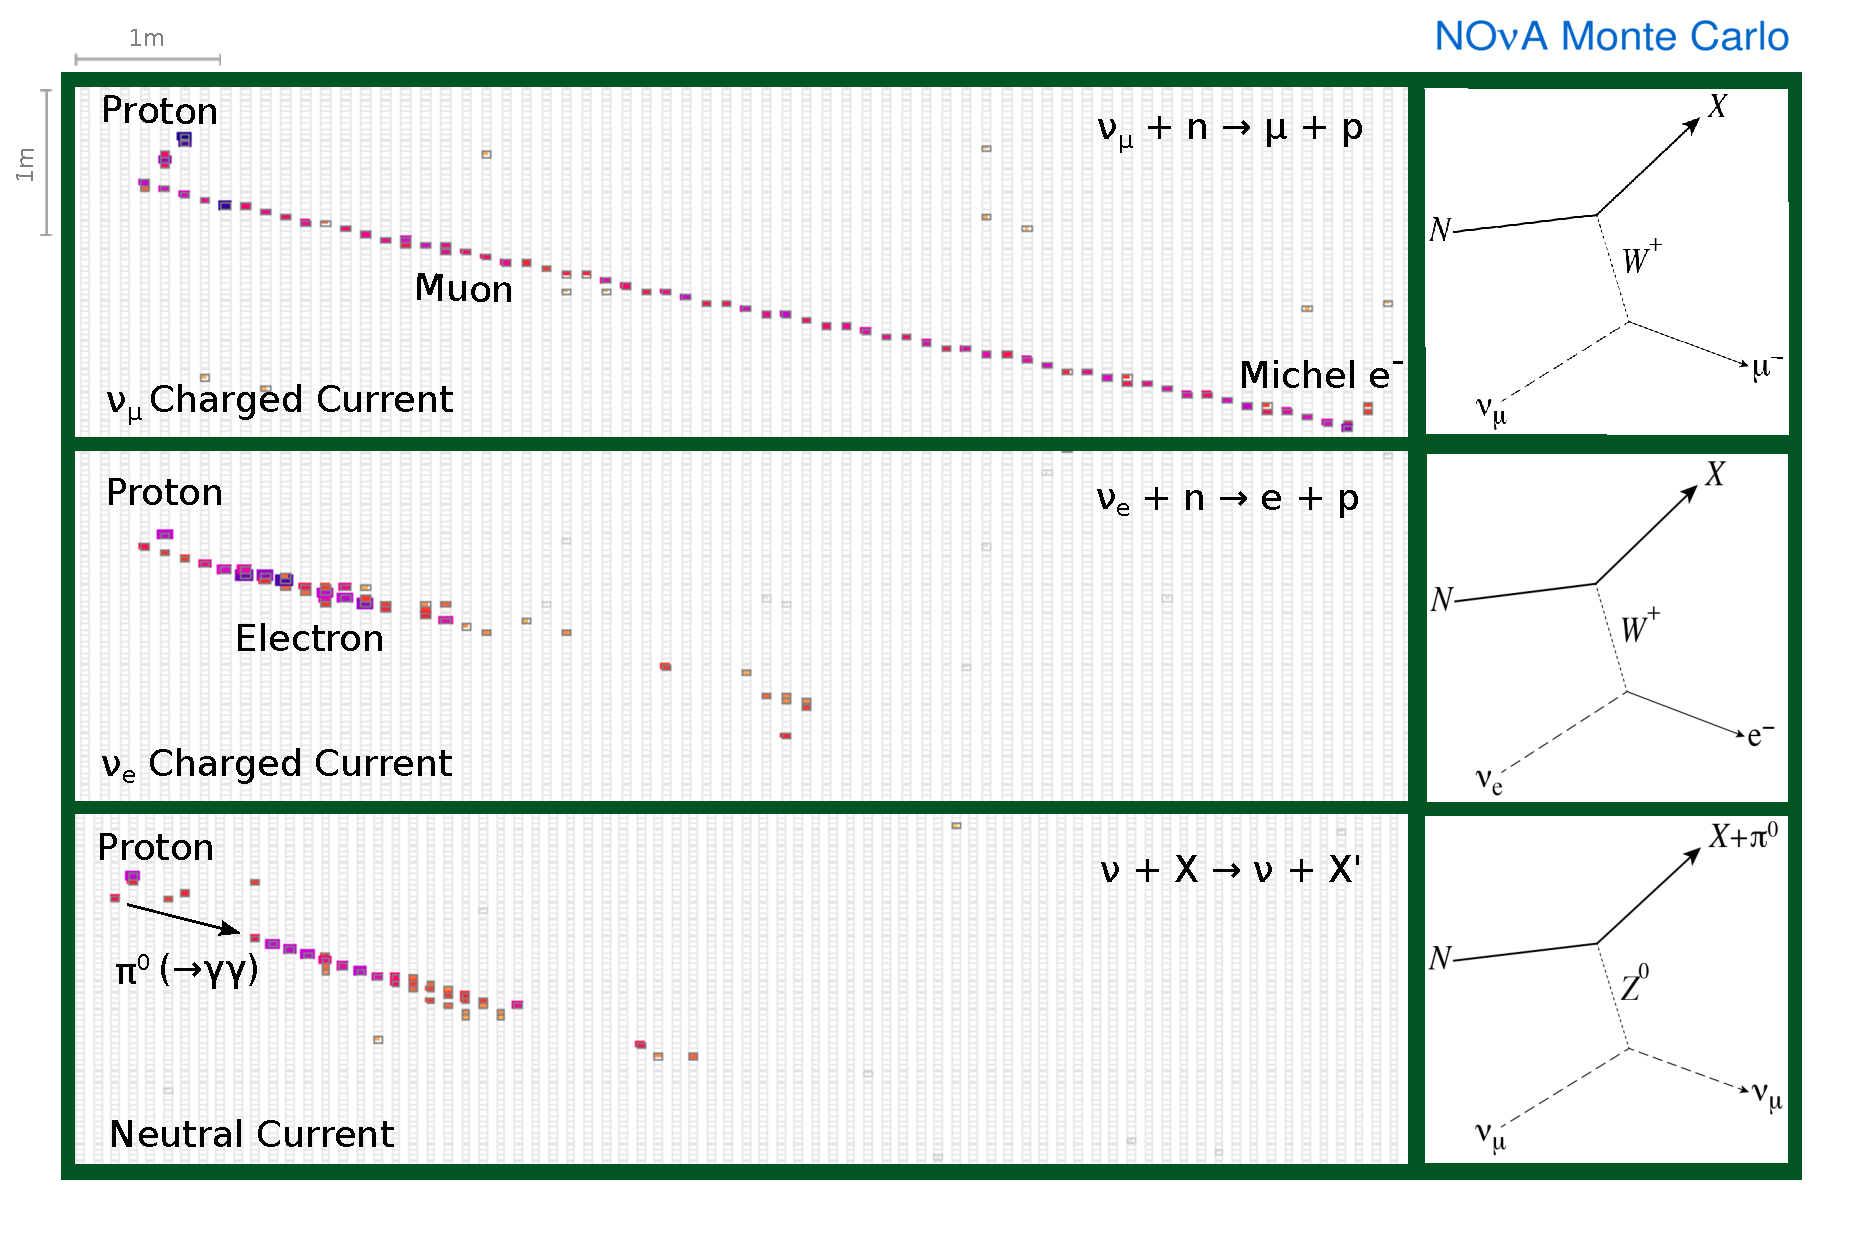
\includegraphics[width=1\textwidth]{/home/robert/Documents/School/PhD/Thesis/Plots/NOvAExperiment/NOvAEventTopology.pdf}
\caption[NOvA detectors event topologies]{Different event topologies as seen in the \acrshort{NOvA} detectors with corresponding Feynman diagrams \cite{NOvAReco.pdf}. Each event is a simulated $\unit[2.15]{GeV}$ neutrino interacting in a \acrshort{NOvA} detector producing a $\unit[0.78]{GeV}$ proton and a second $\unit[1.86]{GeV}$ particle depending on the interactions type. The figure show one view and the colouring represents the deposited energy.}
\label{fig:NOvAEventTopologies}
\end{figure}

NOvA employs a \gls{CNN} based on the GoogLeNet \cite{GoogLeNetArchitecture.pdf} architecture named \gls{CVN} \cite{CVN.pdf}, which uses slice hits to classify interactions into one of the four categories: $\nu_e$, $\nu_\mu$, $\nu_\tau$, \gls{NC}, or cosmic. Since this algorithm identifies the entire event it is also sometimes called \textit{EventCVN}. The same architecture, but applied to the Fuzzy-K prongs and called \textit{ProngCVN} \cite{PsihasNOvAThesis_ProngCVN.pdf}, is used to identify the individual prongs based on what particles they most likely correspond to. This is useful to assign in the calculation of the prong energy, as described in Sec.~\ref{sec:NOvAEnergyEstimation}. A special \gls{ML} algorithm for identifying muons, based on a \gls{BDT} with inputs from the Kalman track, is called \gls{ReMId}~\cite{RaddatzNOvAThesis_KalmanTracks.pdf}.

%From First NOvA results on FHC+RHC: These clusters are categorized as electromagnetic or hadronic in origin using a convolutional neural network (CNN) [Fernanda Psihas thesis]. Hits forming tracks are identified as muons by combining information on the track length, dE=dx, vertex activity, and scattering into a single particle identification (PID) score [Raddatz thesis].

%From NOvAHalfTimeOverview2022.pdf: The energy of charged current neutrino interactions is estimated from the sum of energies of the lepton and the hadronic recoil system. A Kalman-like algorithm is used with a BDT based on energy loss, multiple scattering, and length parameters of a candidate track to identify muons and reconstruct their energy using track length. The energy of electron neutrinos is estimated from a quadratic function of the calorimetric energies of the electron candidate and the hadronic recoil system derived from the simulation [33, 34].

%%%%%%%%%%%%%%%%%%%%%%%%%%%%%%%%%%%%%%%%%%%%%%%%%%%%%%%%%%%%%%%%%%%%%%%%%%%%%%%
%%%%%%%%%                   Detector calibration                     %%%%%%%%%%
%%%%%%%%%%%%%%%%%%%%%%%%%%%%%%%%%%%%%%%%%%%%%%%%%%%%%%%%%%%%%%%%%%%%%%%%%%%%%%%
\section{Detector Calibration}\label{sec:NOvACalibration}
%%% General introduction to calibration - why do we do calibration? What do we get from the DAQ?
The energy deposited within the NOvA detectors is represented by the peak \gls{ADC} values for each cell the particle passed through, which are obtained from the readout electronics, as described in Sec.~\ref{sec:DAQ}.
To convert \gls{ADC} into physical units we need to calibrate the \gls{NOvA} detectors \cite{PrabhjotNOvAThesis_CalibrationAndOscResults2019.pdf}, while accounting for the attenuation of light along the \gls{WLS} fibres, or for differences between individual cell. The purpose of calibration is to calculate a conversion factor from $\unit{ADC}\rightarrow\unit{MeV}$ units, so that the same energy deposited at any place within any detector and at any time, is recorded as the same value.
%By doing this individually for each cell and for small periods at a time, we ensure that energy deposited in any detector, at any place within the detector and at any time, is recorded as the same value in physical units.

%From NOvAHalfTimeOverview2022.pdf: The variations in light output between cells and those due to attenuation along the readout fiber, in both data and simulation, are calibrated using cosmic-ray muons. The overall energy response of the detectors is calibrated using stopping muon tracks along a window from 200 cm to 100 cm before the end of the track. The absolute energy scale is cross-checked and bench marked against simulation using beam-induced protons, muons, and neutral pions at the Near Detector.

%make sure that we get the same amount of energy wherever or whenever it's deposited in whichever of NOvA's detectors and to express this amount of energy in physical units. The NOvA calibration uses cosmic ray muons, which provide a consistent, abundant, and well-understood source of energy deposition.

%%% Calibration samples, trigger, reconstruction, and selection. Also simulation, fiber brightness and so on...
\gls{NOvA} uses cosmic ray muons for calibration due to their abundance in the \gls{NOvA} detectors and a consistent energy deposition. We use hits from a subsample of muons stopping inside the detectors, from a window when they are almost exactly \gls{MIP}, to calculate the absolute energy scale. The cosmic muons are collected using a periodic trigger with the same length as the beam trigger, removing events with timestamps overlapping with the beam spill window. For the simulation of cosmic muons we use the \gls{CRY}~\cite{CRY} \gls{MC} generator, as outlined in Sec.~\ref{sec:NOvASimulation}.

%[NOvAResultsNuOnly2018.pdf] Separate periodic minimum-bias triggers of the same length as the beam trigger allow us to collect high-statistics cosmic data for algorithm training and calibration purposes.

\note{I talk about this selection later on in the Test Beam calibration chapter when I talk about the data-based simulation. Should I therefore elaborate more on this or is this enough?}
We reconstruct the cosmic muon tracks using the window cosmic track algorithm explained in Sec.~\ref{sec:NOvAReconstruction}. To select good quality cosmic tracks we require that at least $80\%$ of all hits from the reconstructed slice contribute to the track \cite{NOvA-doc-13579-FACalorimetricEnergyScale}. Additionally, all tracks must cross at least $\unit[70]{cm}$ along the z axis and must have at least $20\%$ of their total track direction in the z axis, since very vertical tracks tend to not be reconstructed well. \note{There are additional selection criteria which are not as important, do I need to mention them?}. To select stopping muons we look for Michel electrons, which get produced by decaying muons at the end of their tracks, as can be seen on the top panel of Fig.~\ref{fig:NOvAEventTopologies}.

Since the energy deposited in a cell is proportional to the distance the particle travels through the cell, we use the value of the deposited energy divided by the path length through the cell as the input variable for calibration. To ensure we use precise estimate of the path length, we only use hits that satisfy the \textit{tri-cell} condition, shown in Fig.~\ref{fig:NOvATricellCondition}. This means that for each hit there must be a corresponding hit in both of the surrounding cells in the same plane for the same track. This allows us to calculate the path length simply from the height of the cell and the angle of the reconstructed track. In case there is a bad channel in a neighbouring cell (right side of Fig.~\ref{fig:NOvATricellCondition}), we ignore this channel and look one cell further. We can then calculate the path length simply as the cell width divided by the cosine of the direction angle \cite{PrabhjotNOvAThesis_CalibrationAndOscResults2019.pdf}. In case the tricell condition fails, we also evaluate the \textit{`Z tricell'} condition, which requires a hit in both neighbouring planes in the same cell and in the same view. These `Z tricell' hits are saved in a separate histogram and are only used if there are no hits that would satisfy the original tricell condition. This is especially useful for the cell on the edge of the detector, which fail the tricell condition be design, as they only have one neighbouring cell in the same plane.

\begin{figure}[hbtp]
\centering
\begin{subfigure}[b]{0.49\textwidth}
\centering
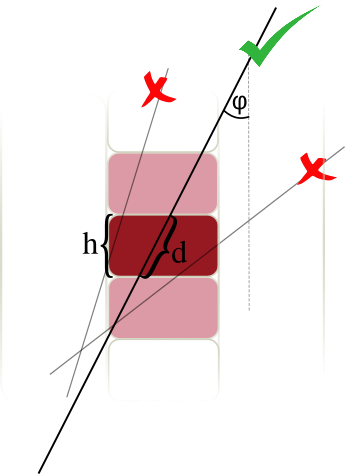
\includegraphics[width=0.6\textwidth]{Plots/NOvAExperiment/TricellConditionWithDescription.png}
\end{subfigure}
\begin{subfigure}[b]{0.49\textwidth}
\centering
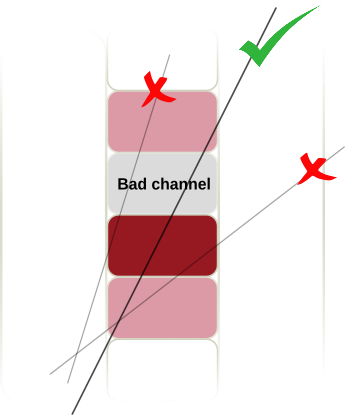
\includegraphics[width=0.6\textwidth]{Plots/NOvAExperiment/TricellConditionWithBadChannel.png}
\end{subfigure}
\caption[Tricell condition for calibration hits in NOvA]{Illustration of the tricell condition. We only use hits that have two surrounding hits in the same plane to be used in the \acrshort{NOvA} calibration, shown on the left plot. This is to ensure a good quality of the path length (d) reconstruction, which is calculated from the known cell height (h) and the reconstructed track angle $\left(\varphi\right)$. In case the hit is next to a bad channel, as shown on the right plot, we ignore this bad channel and require a hit in the next cell over.}
\label{fig:NOvATricellCondition}
\end{figure}

%The first step in the attenuation calibration is to select the suitable hits from tracks of cosmic ray muons. Because a reliable estimate of pathlength is required, not all hits are suitable for use.  If a cell has each of its neighbors in the same plane hit, then we know, for a Y view cell, that the track entered through the upper wall, and exited through the lower wall. The pathlength then is just the width of the cell divided by the direction cosine. This selection also significantly decreases the chance that the hit in question is a noise hit. Allowance is made for neighboring dead cells, so e.g. “hit, dead, hit, hit” would still lead the 3rd cell to be selected. The second best hit selection, in cases where there are too many dead neighboring cells on each side, is the so-called “z” estimator, where a hit is required at the same cell number in each of the neighboring planes in the same view. The pathlength is then the ratio of cell depth to cz.[docdb:13579 - SA The Attenuation and Threshold Calibration of the NOvA detector, copied from docdb:7410]

%from docdb:7410: A requirement that the track be “throughgoing” (lowest endpoint outside the fiducial volume) was applied, but doesn’t make much difference. I think this selection was broken by the recent changes to StopperSelection anyway. (So it seems that it was required for the relative calibration that the muons are through-going, but I assume this was discarded somewhere down the line)

%Stopping muon selection (from docdb:13579 - FA\_Calorimetric\_energy\_scale): There are two avenues for selecting stopping muons; i) selecting tracks whose reconstructed end point is contained within the detector and ii) selecting tracks that have a Michel electron at one end. Michel electrons are useful for both identifying muons and effective tagging of the end point of muon tracks. The stopping selection requires the reconstructed end point of the muon track to be at least 50 cm from the detector edge. The identification of a Michel electron at the end of a muon track has two stages of both temporal and spatial range requirements. Firstly, a candidate Michel electron hit is required to occur between 1 and 30 microseconds after the mean time of the hits on the track. Furthermore, the candidate Michel electron must be within a 30 cm sphere surrounding the reconstructed track end point. The candidate Michel electron hit for a muon track is the hit that produces the largest detector response among the hits that pass the above cuts. Secondly, cell hits surrounding the candidate Michel electron hit are associated with the Michel electron if they occur within a 30 cm sphere surrounding the Michel electron candidate. Furthermore, to be associated with the Michel electron the cell hits must occur between 0.5 microseconds before and 0.5 microseconds after the candidate Michel electron. Michel electrons at the end of muon tracks are reconstructed using the candidate and associated Michel electron hits. The stopping muon selection requires a Michel electron at the end of the muon track.

%Calibration is necessary to convert electronic signals to physically meaningful energy in units of GeV. Two calibration steps precede the calorimetric energy calibration. First raw ADCs (Analogue Digital Conversion) are converted to units of photo-electrons (PE) using the known average response of the APDs; secondly an attenuation calibration corrects for the position dependent response [6]. A drift calibration may be included in the future to correct for changes in detector response over time. The calorimetric energy scale calibration is the last step in the calibration chain and the detector response should already be uniform in space and eventually also in time. [docdb:13579 - FA\_Calorimetric\_energy\_scale]

%Using the average expected APD response, integrated charge from the ADCs are converted to units of photo-electrons (PE) [SA Absolute energy scale]

The calibration conversion factor from the signal recorded by the detector readout and the actual deposited energy can be expressed by Eq.~\ref{eq:NOvACalibration}.
\begin{equation}\label{eq:NOvACalibration}
E_{dep}\ \left[\unit{MeV}\right]=\textsf{Signal}\ \left[\unit{ADC}\right]\times S_d\times TS_{d,i}\times R_{d,i}\left(t\right)\times A_d\left(t\right).
\end{equation}
Here we can see that calibration consists of four separate and complementary factors: the Scale $\left(S_d\right)$, the Threshold/Shielding correction $\left(TS_{d,i}\right)$, the Relative calibration $\left(R_{d,i}\left(t\right)\right)$ and the Absolute calibration $\left(A_d\left(t\right)\right)$, all described below. Each part is calculated for each detector separately, as indicated by the subscript $d$. The Relative and Absolute calibrations are calculated for each time period separately to account for possible changes in the energy deposition throughout the time, possibly caused by the ageing of the scintillator oil, or of the readout electronics. The time periods are either determined by running conditions and separated by significant changed to the readout or \gls{DAQ} systems, including the summer shutdown, or by a fixed time interval.

The Threshold/Shielding correction and the Relative calibration calculate a calibration factor for each position within the detector to account for variations caused by the attenuation of light as it travels through the \gls{WLS} fibres, or by differences between individual cells. This is denoted as a subscript $i$ in Eq.~\ref{eq:NOvACalibration}. For data, the position of hit in a detector is described by the plane number, the cell number and the position within the cell $\left(w\right)$. $w$ is calculated as the projection of the cosmic track to the central cell axis and its value is equivalent to the X axis (Y axis) coordinate of the projection for the horizontal (vertical) cells, with the 0 value at the centre of the cell \cite{PrabhjotNOvAThesis_CalibrationAndOscResults2019.pdf}.

%The light is attenuated while traveling through the fiber. To find the correct energy of the incident particle these losses are corrected by using cosmic ray muons. The cosmic ray muons are used to calibrate the NOvA detectors because they provide a source of consistent energy across the detectors. The purpose of the attenuation calibration is to provide constants and formulae such that an amount of energy deposited in the detector and registered by an APD can be expressed in comparable units, PECorr which are the corrected photo-electrons (PE) no matter where the deposition occurred. Variations in time are to be handled by the drift calibration. The purpose of the absolute calibration is to provide a scaling factor, independent of channel since all of that variation should have been taken out by the relative calibration, so that energy deposits can be expressed in physically meaningful units (GeV).
%For both purposes cosmic rays are used as probes. For the attenuation calibration they represent a source of consistent energy deposits across the detector of approximately 1 minimum ionizing particle’s energy, MIP, but this is not assumed. Any average value consistent across the detector would do. For absolute calibration, stopping muons are used, whose precise energy deposits should be estimateable from the Bethe Bloch formula. [docdb:13579 - SA The Attenuation and Threshold Calibration of the NOvA detector, but a lot of this is actually just copied from Backhouse's original calibration technote docdb:7410]

%(Dividing data into periods and epochs) A new period is started for a major change to running conditions such as a horn current change, a long shutdown, target replacement, etc. Periods are divided into epochs. A new epoch is started whenever analysis or production reasons dictate. Calibration has been performed for all the periods separately and has used the data that are determined by the Data Quality group to be good. The effects of aging, temperature, partial filling, and cooling are neglected. The drift calibration should be able to account for all of these (but drift calibration doesn't really exist yet afaik). [docdb:13579 - SA The Attenuation and Threshold Calibration of the NOvA detector]

For simulation, we do not use the plane number to determine the position within a detector, as by construction all detector planes should have the exact same readout. This significantly reduced the requirements for the number of events that need to be simulated, reconstructed and calibrated, especially for the \gls{FD} with 896 planes. However, in reality there are some variations in detector response between individual planes, caused by different \textit{brightness} qualities of the fibres, zipped or twisted fibres, different qualities of the scintillator, possible air bubble, or potentially others. Since we want to include these differences into simulation without having to simulate every cell individually, we divide all cells into 12 equally populated \gls{FB} bins based on
the uncorrected average response in the center of that cell, as shown in Fig.~\ref{fig:NOvAFiberBrightness}. These brightness bins describe the relative differences in the detector response between individual cells \cite{NOvA-doc-34909}.

%\cite{NOVA-doc-13579-SAAttenuationAndThreshold,NOVA-doc-34909}.

\begin{figure}[hbtp]
\centering
\begin{subfigure}[b]{0.495\textwidth}
\centering
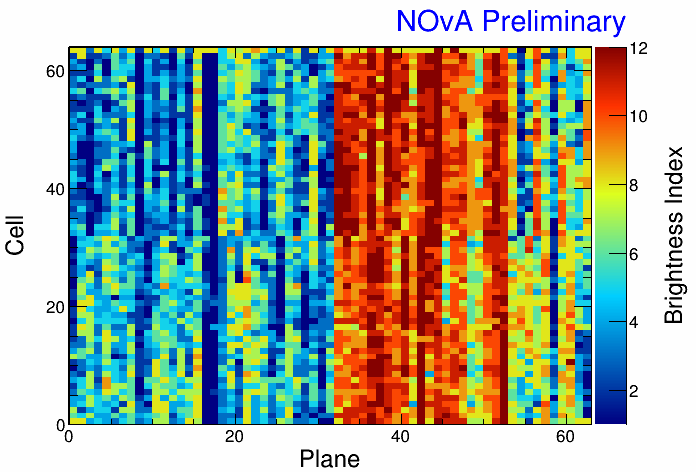
\includegraphics[width=\textwidth]{Plots/NOvAExperiment/BrightnessIndex.png}
\end{subfigure}
%\hfill
\begin{subfigure}[b]{0.495\textwidth}
\centering
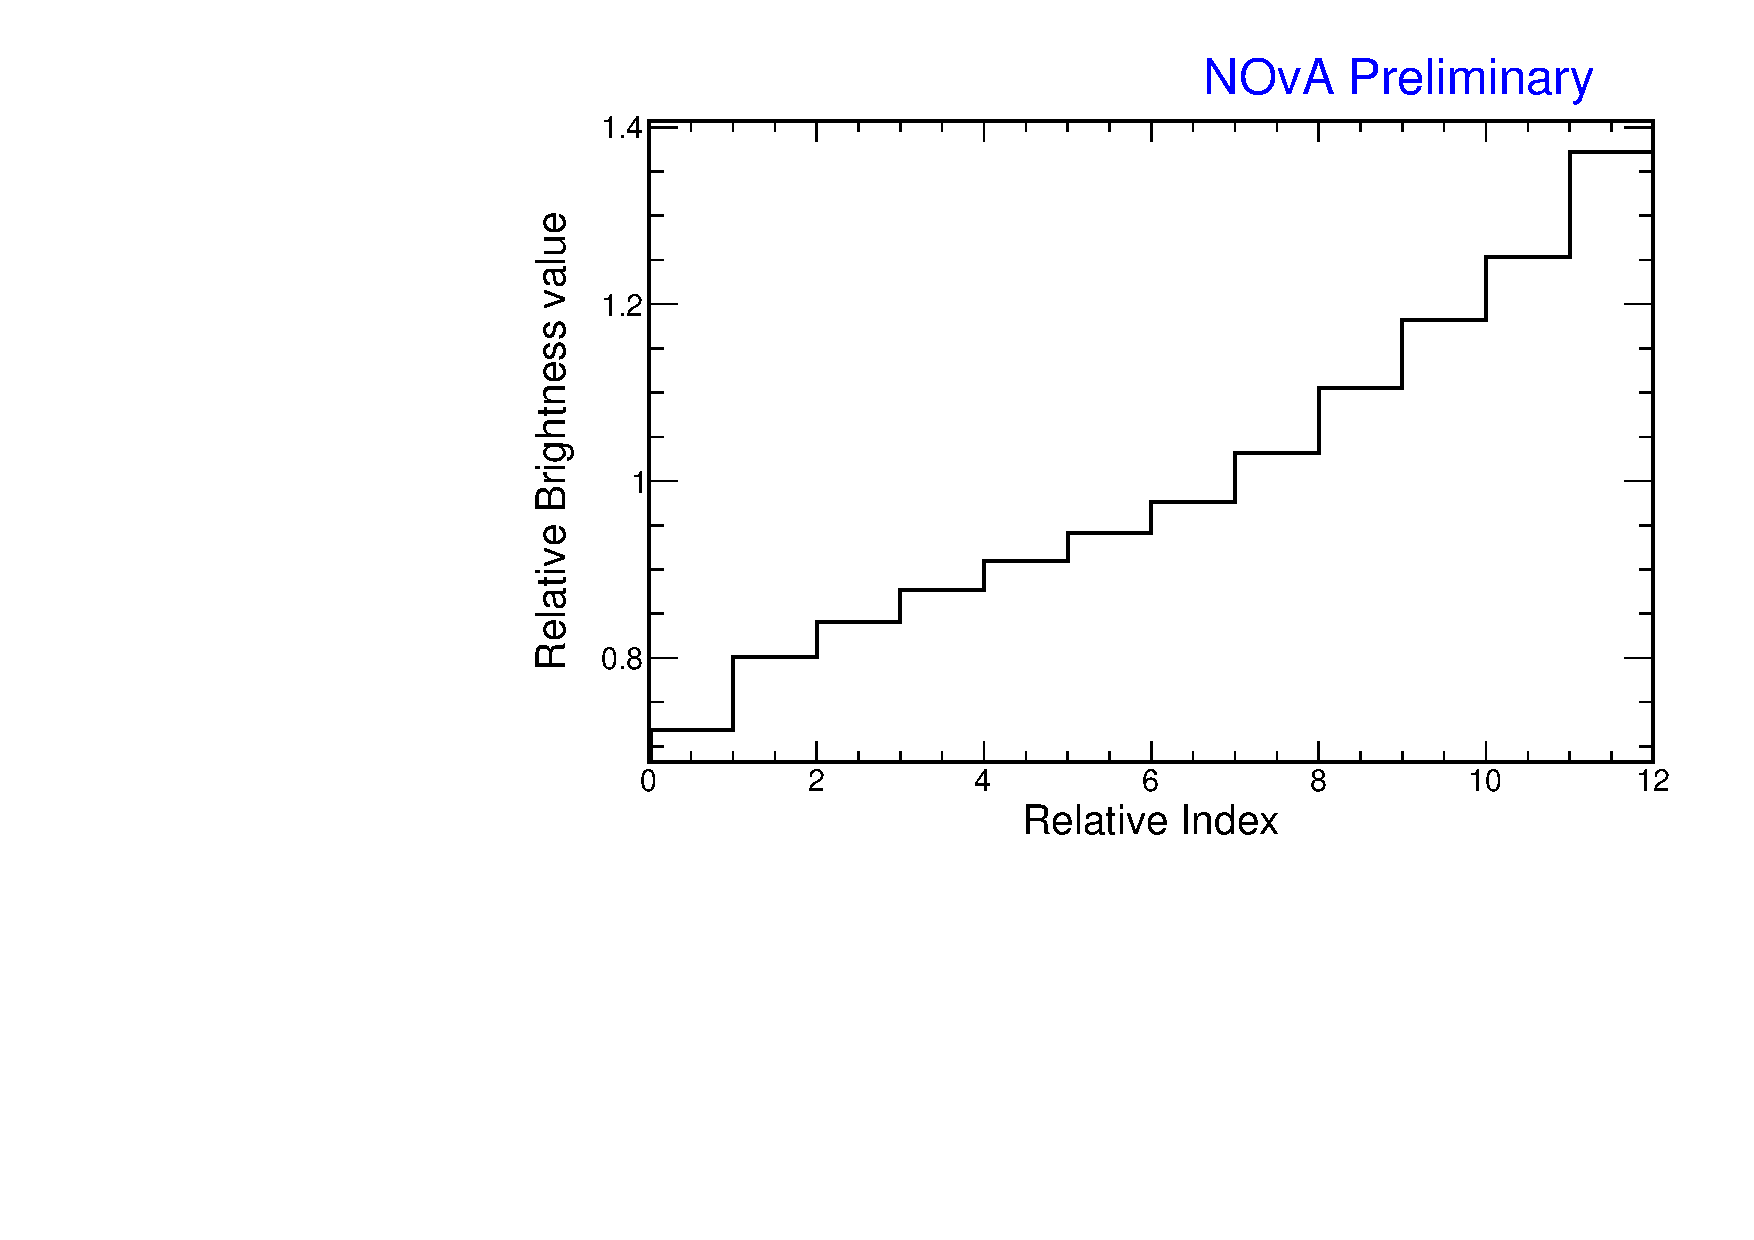
\includegraphics[width=\textwidth]{Plots/NOvAExperiment/BrightnessIndexToValue.pdf}
\end{subfigure}
\caption[Fibre Brightness bins for the NOvA calibration]{Distribution of the \acrshort{NOvA} detector cells into 12 brightness bins (left plot), each representing a relative difference in energy response (right plot) due to different brightnesses of the fibres, scintillators, or readout. This is an example from the \acrshort{NOvA} Test Beam detector, where the left side of the detector (planes 1-32) has clearly lower response relative to the right side of the detector (planes 33-64).}
\label{fig:NOvAFiberBrightness}
\end{figure}

%To divide each detector into the 12 brightness bins, we use results from the relative calibration. Specifically we take the result of the attenuation fit (equal to the average response) in the centre of each cell to fill a 2D histogram. Then we normalize this histogram by dividing the response in each $\textsf{Cell}\times\textsf{View}\times\textsf{Plane}$ by the average response in the corresponding $\textsf{Cell}\times\textsf{View}$. All uncalibrated cells get assigned the average response (1 in normalized histogram). Then we make a 1D histogram filled with the normalized responses of each cell and divide this histogram into 12 equally populated bins (so each bin represents approximately the same number of detector cells, shown on the left plot of Fig. \ref{figFiberBrightnessBins}). The mean normalized response in each bin represents the relative brightness value of this bin (right plot of Fig. \ref{figFiberBrightnessBins}).

\subsection{Scale}
The Scale calibration factor from Eq.~\ref{eq:NOvACalibration} is a simple conversion from the peak \gls{ADC} value into the number of \gls{PE}s. This factor only depends on the \gls{APD} gain (which was different in the beginning of \gls{NOvA} data taking) and on the FEB type (different between detectors, as described in Sec.~\ref{sec:DAQ}).

%I think I should actually include some kind of a description of the ADC to PE conversion.
\iffalse
The scaling of the ADC to PE depends only on the gain and the version of the FEB. Otherwise it's just a very simple scaling (explain this at the PE definition):
\begin{equation}
PE=\frac{\textsf{peakADC}}{\textsf{ADCPerPE}},
\end{equation}
\begin{equation}
\textsf{ADCPerPE}=\textsf{Gain}\times\frac{4095}{ADCScale}
\end{equation}
where ADCScale is 217000 for FEBv4.1 and 204800 for FEBv5.2.
\fi

%The PECorr scaling is 75.0 (NDOS), 37.51 (ND), 39.91 (FD) and 39.91 (TB)

\subsection{Threshold and Shielding Correction}
%[CalibrationFirstTechnote2014.pdf] There are three main assumptions for calibration: response is stable in time (drift), the energy spectrum of cosmic rays is uniform in space (shielding), the ADC response to arriving photons is linear

The Threshold and Shielding correction accounts for two assumptions, which hold true in most cases in NOvA, but fall short for some hits at the bottom of the detector, or far away from the readout, especially for the \gls{FD} \cite{PrabhjotNOvAThesis_CalibrationAndOscResults2019.pdf}. The first assumption is that the \gls{ADC} response to the photon signal is linear, which is mostly true except close to the \gls{APD} threshold. Energy deposited far away from the readout may produce photons that get attenuated enough to be shifted below the threshold. However, due to natural fluctuation, the same deposited energy may also produce photons that would make it over the threshold, therefore making it appear that the actual deposited energy was higher then in reality, introducing a bias to the calibration. The threshold correction is calculated using simulation, as the ratio between the number of simulated \gls{PE} seen by the \gls{APD} $\left(\textsc{PE}_{true}\right)$ and the Poisson mean number of simulation photons created in the scintillator by the same deposited energy $\left(\lambda\right)$.

The second assumption is that the spectrum of cosmic muons is uniform within each detector. Again, this is generally true, but breaks down at the \gls{FD}, which is big enough that the top of the detector shields the bottom part of the detector and affects the energy distribution. The shielding correction is calculated from simulation as a ratio between the true energy deposited by a charged particle $\left(E_{true}\right)$ and the expected deposited energy if the particle was \gls{MIP} $\left(E_{\textsc{MIP}}\right)$. 

The total Threshold and Shielding correction is calculated for simulated events in each cell, \gls{FB} bin and $w$ position according to Eq.~\ref{eq:NOvAThresholdShieldingCorrection}. The final correction is a fit to the mean correction value along $w$ in each cell and \gls{FB} bin.

\begin{equation}\label{eq:NOvAThresholdShieldingCorrection}
TS_i = \frac{\textsc{PE}_{true}}{\lambda}\frac{E_{true}}{E_{\textsc{MIP}}}
\end{equation}

%Similar effect, specifically for the vertical cells, is caused by using cosmic muons for calibration and applying it to beam muons. The top of the detector effectively shields the bottom, skewing the energy distribution of cosmic muons. To correct for both of these effect, we use the simulation pclist sample to calculate the threshold and shielding (also called threshold and shadowing) correction by comparing the true and reconstructed information. We apply this correction before the attenuation fits \cite{NOVA-doc-13579-SAAttenuationAndThreshold}.

%Should I write anything more? Maybe about how do we calculate this more specifically, or that it's done for view X fb bin X cell X w

%In the Far Detector data and MC a large divergence between calibrated and true energies as a function of W was observed [8]. This was traced back to the much longer cell lengths in the FD meaning that thresholds play a large role at the foot of a cell. Also self-shielding of the detector by its own mass lay a role in the observed discrepancy. Thresholds mean that for a hit to be seen by an APD, it may need to have a slight upwards fluctuation in the number of photons produced by the energy deposition. Self-shielding means that the average visible energy depositions from MIPs are not truly spatially uniform in the detector. If not corrected for these effects, there will be a bias in the set of hits that the attenuation fit sees, and leads it to overestimate the light-level, and so under-estimate real hit energies by tens of percent. The approach adopted to solve this problem was to create a correction factor as a function of view, cell, and position along the cell which would be applied before the attenuation correction to remove the effect of thresholds and shielding. To this end MC truth information about the calibration hit sample is used to create a combined threshold and shadowing correction for each cell and view combination,
%\begin{equation}
%T=\frac{PE}{\lambda}\frac{E_{true}}{E_{mip}},
%\end{equation}
%where $T$ is the combined “threshold and shielding” correction factor, $PE$ is the simulated photoelectrons recorded at the readout, $\lambda$ is the number of simulated photons which would be seen at the readout out in the absence of fluctuations, $E_{true}$ is the true energy deposited in the cell and $E_{mip}$ is the naive energy you would expect to be deposited based on the pathlength through the cell. In this way it encodes a threshold correction based on the simulated readout PE with and without the fluctuations, with $\lambda$ dependent on your simulated threshold, as well as a shielding correction based on the simulated energy deposition and a naive no shielding approximation. This equation gives us a cell by cell correction but we use an empirical polynomial fit to that distribution which removes statistical noise from the correction and well describes the initial distribution. This correction factor is applied to the cell by cell data and MC PE/cm distributions before the attenuation fits. [docdb:13579 - SA The Attenuation and Threshold Calibration of the NOvA detector, reference 8 is for docdb:7247, a talk by Backhouse]

\subsection{Relative Calibration}\label{secRelativCalibration}

%The \textbf{relative calibration} corrects for attenuation of scintillator light as it travels through the cell to the readout, as well as for differences between detector cells. This correction is calculated for each cell separately.

%Detailed description can be found in the "Instructions for the Attenuation Calibration Job" technote from Prabhjot from docdb:13579 (list of all calibration technotes) and on the relative calibration wiki page.

Relative calibration corrects mainly for the attenuation of the scintillator light as it travels through the \gls{WLS} fibre to the readout. Since to correction is calculated for each cell independently, it effectively correct for the relative differences between detector cells as well. The result of the Relative calibration is the detector response to a particle in the units of \gls{PECorr}, which is calculated as the ratio between an average response in \gls{PE} across the entire detector (can differ across detectors) and the result of the \textit{`attenuation fit'} in that particular position within the detector. This way the \gls{PECorr} should be uniform across the detector along the plane number, cell number and $w$ distributions \cite{PrabhjotNOvAThesis_CalibrationAndOscResults2019.pdf}.

%by fitting the average detector response over the position in each cell, separately for every cell inside each detector. Dividing the "average response" of the detector by the result of the attenuation fit for each $\textsf{Plane}\times\textsf{Cell}\times\textsf{w}$ combination effectively removes relative differences within and between all cells across the entire detector. The average response is a single constant number chosen to approximately represent the average response in the middle of the cell. Its value is for the far detector and Test Beam 39.91~PE/cm and for the near detector 37.51~PE/cm. The value of the average response has no impact of the calibration results, as the absolute scale of the detector response is determined during the absolute calibration and relative calibration only serves to remove the relative differences \cite{NOVA-doc-7410,NOVA-doc-13579-SAAttenuationAndThreshold}.

To do the attenuation fit, we first create the \textit{`attenuation profiles'} for each detector cell. Attenuation profiles are profile histograms of mean detector response over the travelled path length, in the units of $\textsc{PE}/\unit{cm}$, along the position within the cell. An example attenuation profile is shown in Fig.~\ref{fig:NOvACalibrationAttenuationFit} as black dots. We then apply the Threshold and Shielding correction described above before doing the attenuation fit, which consists of two steps. 

\begin{figure}
    \centering
    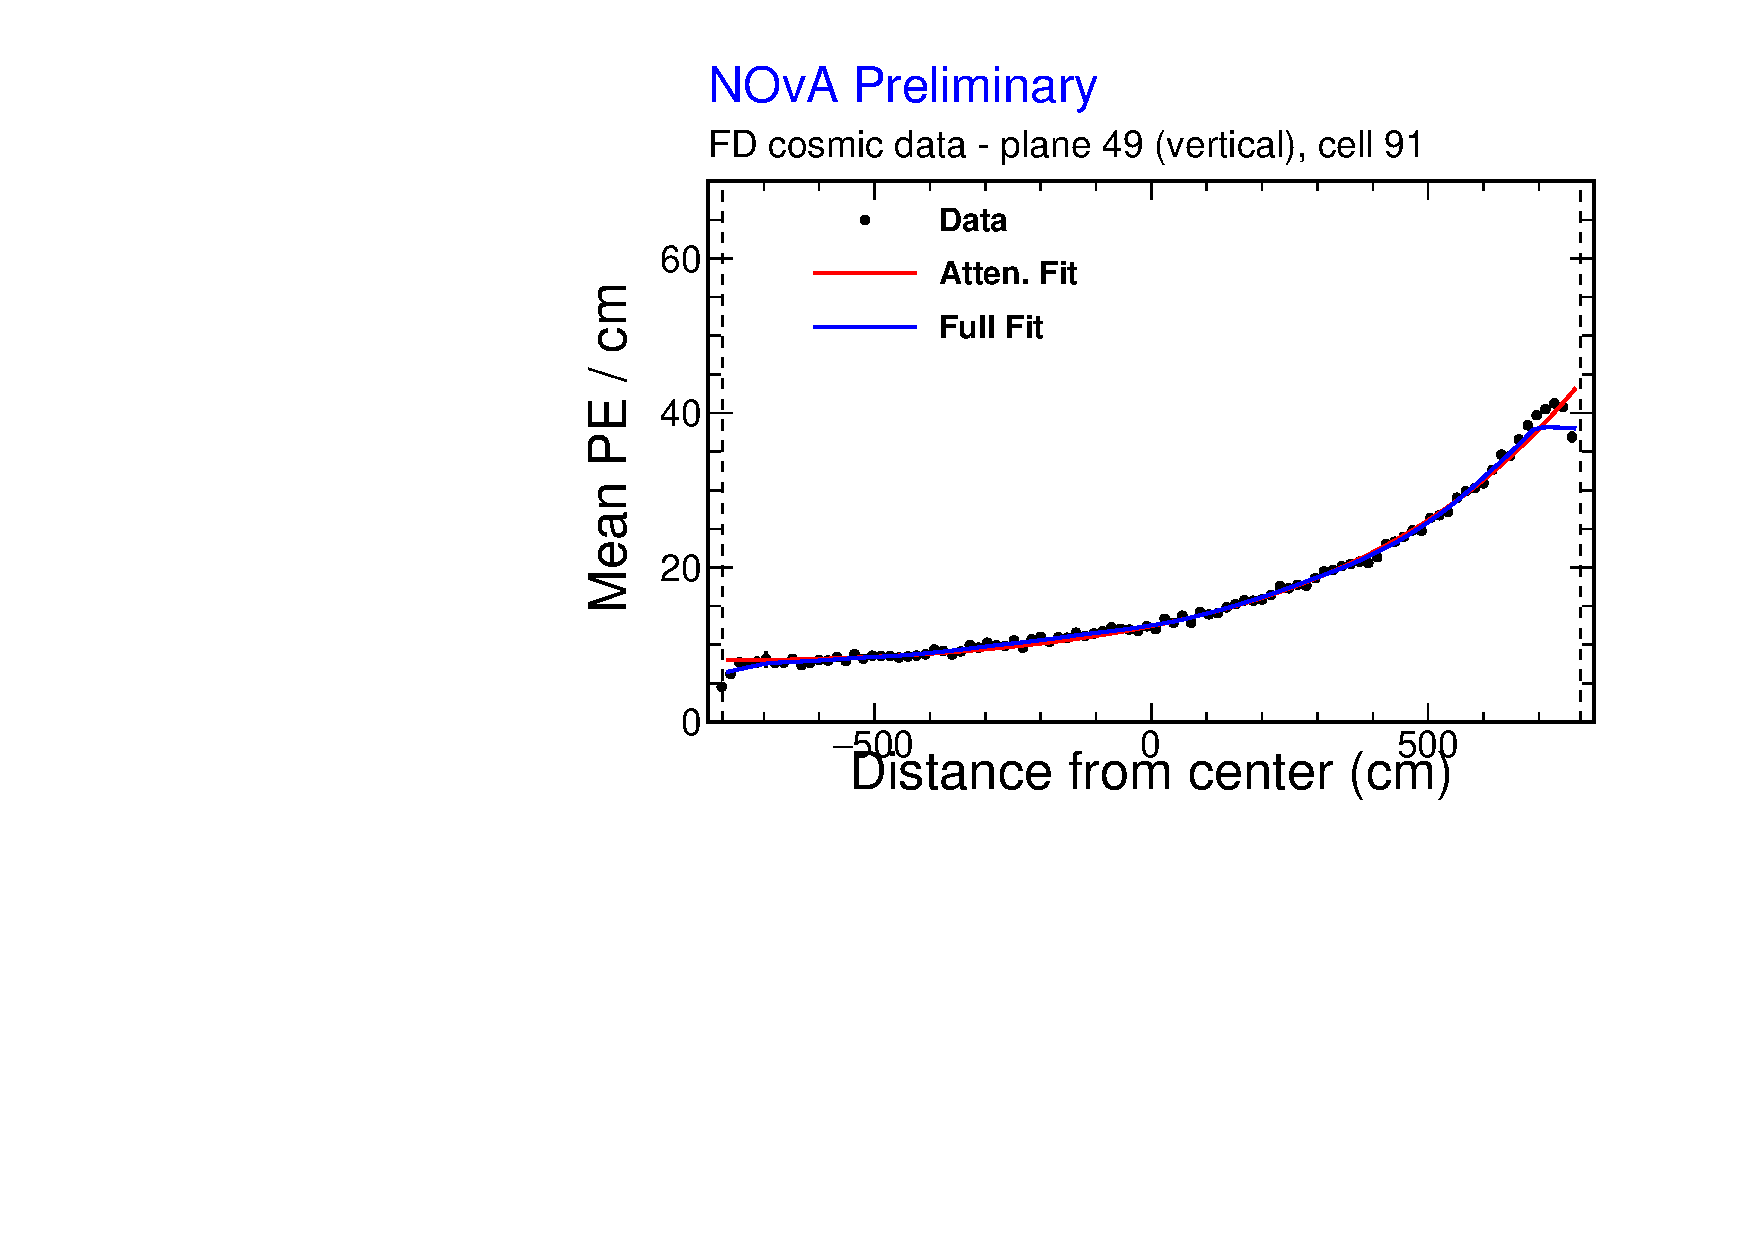
\includegraphics[width=.7\textwidth]{Plots/NOvAExperiment/ExampleAttenuationFit.pdf}
    \caption[Example attenuation fit for NOvA Relative calibration]{Example attenuation fit for a single cell in the \acrshort{NOvA} \acrshort{FD} across its full length, as shown by dashed vertical lines. The red line shows the initial exponential fit and the blue line shows the full fit after the \acrshort{LOWESS} correction, both described in text. Figure from \cite{totfit_fd_datafitX_049_091.pdf}.}
    \label{fig:NOvACalibrationAttenuationFit}
\end{figure}

\begin{enumerate}
\item The first step is a three-parameter exponential fit according to Eq.~\ref{eq:NOvARelCalibExpFit}
\begin{equation}\label{eq:NOvARelCalibExpFit}
y=C+A\left(\exp\left(\frac{w}{X}\right)+\exp\left(-\frac{L+w}{X}\right)\right),
\end{equation}
where $y$ is the fitted response, $L$ is the length of the cell and $C$, $A$ and $X$ are the fitted parameters representing the background, attenuation scale and attenuation length respectively. An example of the exponential fit is shown as a red curve in Fig.~\ref{fig:NOvACalibrationAttenuationFit}.
\item The second step is smoothing out of the residual differences between the exponential fit and the original distribution with the \gls{LOWESS} method, shown in Fig.~\ref{fig:NOvACalibrationLOWESSCorrection}. We use 20 points across the length of each cell to create a smoothed distribution of the residual values. Result of the \gls{LOWESS} correction is then combined with the exponential fit into the full attenuation fit, shown as a blue line in Fig.~\ref{fig:NOvACalibrationAttenuationFit}.
\end{enumerate}

\begin{figure}
    \centering
    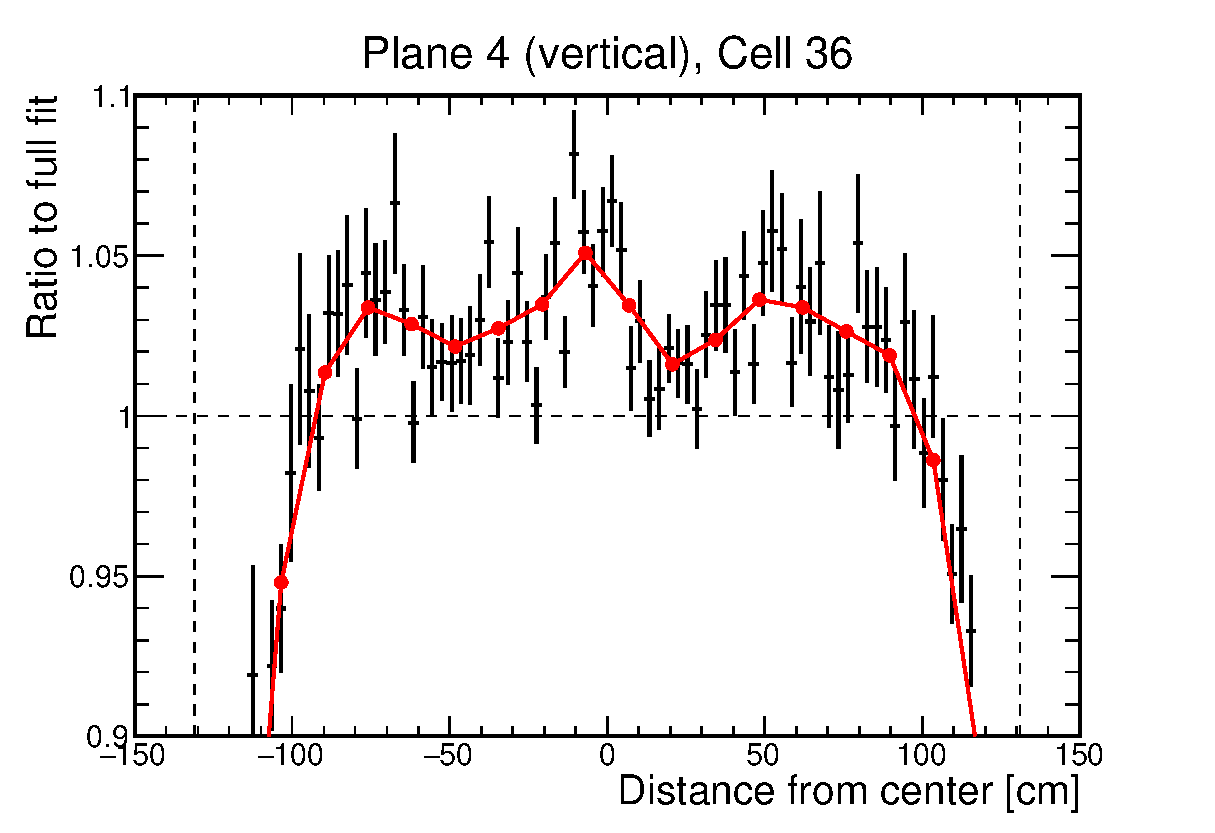
\includegraphics[width=.7\textwidth]{Plots/NOvAExperiment/ExampleLOWESSFit.eps}
    \caption[Example LOWESS correction for NOvA Relative calibration]{Example \acrshort{LOWESS} correction for a the residual differences after the exponential part of the attenuation fit of the \acrshort{NOvA} Relative calibration. This is an example for a single cell in the \acrshort{NOvA} Test Beam detector with black point showing the residual differences and red line the \acrshort{LOWESS} correction, both described in text.}
    \label{fig:NOvACalibrationLOWESSCorrection}
\end{figure}

Even after an application of the \gls{LOWESS} correction, there are sometimes large differences between the attenuation fit and the fitted response. This is usually caused by a small number of events in that cell, common for cell at the edge of the detector. To ensure a good quality of the attenuation fit, we calculate the total $\chi^2$ between the attenuation fit and the fitted response and only call a cell \textit{calibrated}, if the final $\chi^2<0.2$. If $\chi^2>0.2$, we ignore the results for this cell and mark it as \textit{uncalibrated}.

%Attenutation profiles have a constant binnin fNBins=100 (in w), same for ND, FD and TB. This results in an effectively finer binning for TB compared to ND and FD. For FD w = (-900,+900), ND: (-250,+250), TB: (-150,+150). TB: 3cm/bin, ND: 5cm/bin, FD: 18cm/bin. What effect could this have on the relative calibration results? Particularly on the calibration shape?

%where y is the response, L is the cell length, C, A and X are the free parameters in the fit. X gives the attenuation length as well. Initially, the fit is to the central part of the cell, which is different for each detector. In addition to the approximately quartic behavior at the ends of every channel there are in many channels fairly large residuals. They don’t appear to follow any consistent pattern. The leading hypothesis is that these are due to varying fiber position within the cell. Usually the fiber lies in the corners of the cell, but if it is somehow twisted so that it rises into the center of the cell, then it should collect more light, to an extent comparable to what is seen here. To remove such an irregular pattern, the residual from the analytic fit is simply fit with LOcally WEighted Scatter plot Smoothing, LOWESS. The LOWESS curve at each point is formed from the weighted mean of the deviations. The weighting function is the traditional tri-cube, (insert equation, likely not needed for this technote) [docdb:13579 - SA The Attenuation and Threshold Calibration of the NOvA detector, already in 1stAna and Backhouse's technote]

%For NDOS the fit was a very little bit different, where we didn't use $L$ but $3L/2$. Also it says that "Over the length of an NDOS cell, the effect of the long attenuation length is imperceptible, and is modelled as a constant (If you put a long attenuation term in, the fit drives the length scale to infinity anyway). [docdb:7410]

%In many channels, fairly large residuals are visible. They don’t appear to follow any consistent pattern. The hypothesis is that these are due to varying fibre position within the cell. Usually the fibre lies in the corners of the cell, but if it is somehow twisted so that it rises into the centre of the cell, then it should collect more light, to an extent comparable to what is seen here. To remove such an irregular pattern, the residual from the analytic fit is simply fit with LOWESS (locally weighted scatterplot smoothing). The LOWESS curve at each point is formed from the weighted mean of the deviations. The weighting function is the traditional tri-cube:
%\begin{equation}
%w_i=\left(1-\left|\frac{x-x_i}{\sigma}\right|^3\right)^3.
%\end{equation}
%The smoothing length scale $\sigma$ is 30cm. 20 points calculated by this method are stored, to be linearly interpolated between to approximate the full LOWESS curve. If the LOWESS fit at any point exceeds 15\% the original attenuation fit was very bad, and the channel is marked uncalibrated. Figure 4 shows an example of large (10\%) deviations being fitted. This variation is not seen in the MC, and so the LOWESS fit is skipped there. Due to the lower stats available in MC, instead of being collated by plane and cell, the curves are only calculated by view and cell. [docdb:7410]

%The current value of $\sigma$ in the code is $1.5\times\textsf{DetWidth}/20$

\subsection{Absolute Calibration}
%Followed by the \textbf{absolute calibration}, which only uses stopping muons when they are minimum ionising particles. In the absolute calibration we calculate a scale between the measured energy deposition, corrected by the relative calibration, and the simulated energy deposition in physical units of $\unit{MeV}$. This scale is calculated for each time period and each detector separately, which ensures the energy deposition is directly comparable wherever or whenever it occurred.

For the absolute calibration we only use hits from muons stopping inside the detector, $\unit[1-2]{m}$ from the end of their tracks. This is when they are approximately minimum ionizing particles and their energy deposition is well understood. We also remove hits at the edges of each cell, to mitigate the  effects at the end of the \gls{WLS} fibres and the lower number of events at the edge of the detector \cite{NOvA-doc-13579-FACalorimetricEnergyScale}.

We apply the results of the relative calibration to the selected hits to get the  distribution of the corrected detector response in the units of $\gls{PECorr}/\unit{cm}$, as shown on the left of Fig.~\ref{fig:NOvACalibrationAbsoluteEnergyScale}. We then take the mean of this distribution, separately in each of the two views, and in each time period and simulation version, which we call the \textit{reconstructed} \gls{MEU}. Analogously, we take the mean of the true deposited energy in the units of $\unit{MeV/cm}$ from simulation, shown on the right of Fig.~\ref{fig:NOvACalibrationAbsoluteEnergyScale}, and call it the \textit{true} \gls{MEU}. We then take the average over the two views and calculate the absolute energy scale for each time period and simulation version as the ratio on Eq.~\ref{eq:NOvAAbsEnergyScale}.
\begin{equation}\label{eq:NOvAAbsEnergyScale}
\textsf{Absolute Energy Scale} = \frac{\textsc{MEU}_{True}\ \left[\unit{MeV/cm}\right]}{\textsc{MEU}_{Reco}\ \left[\unit{\textsc{PECorr}/cm}\right]}.
\end{equation}

\begin{figure}
    \centering
    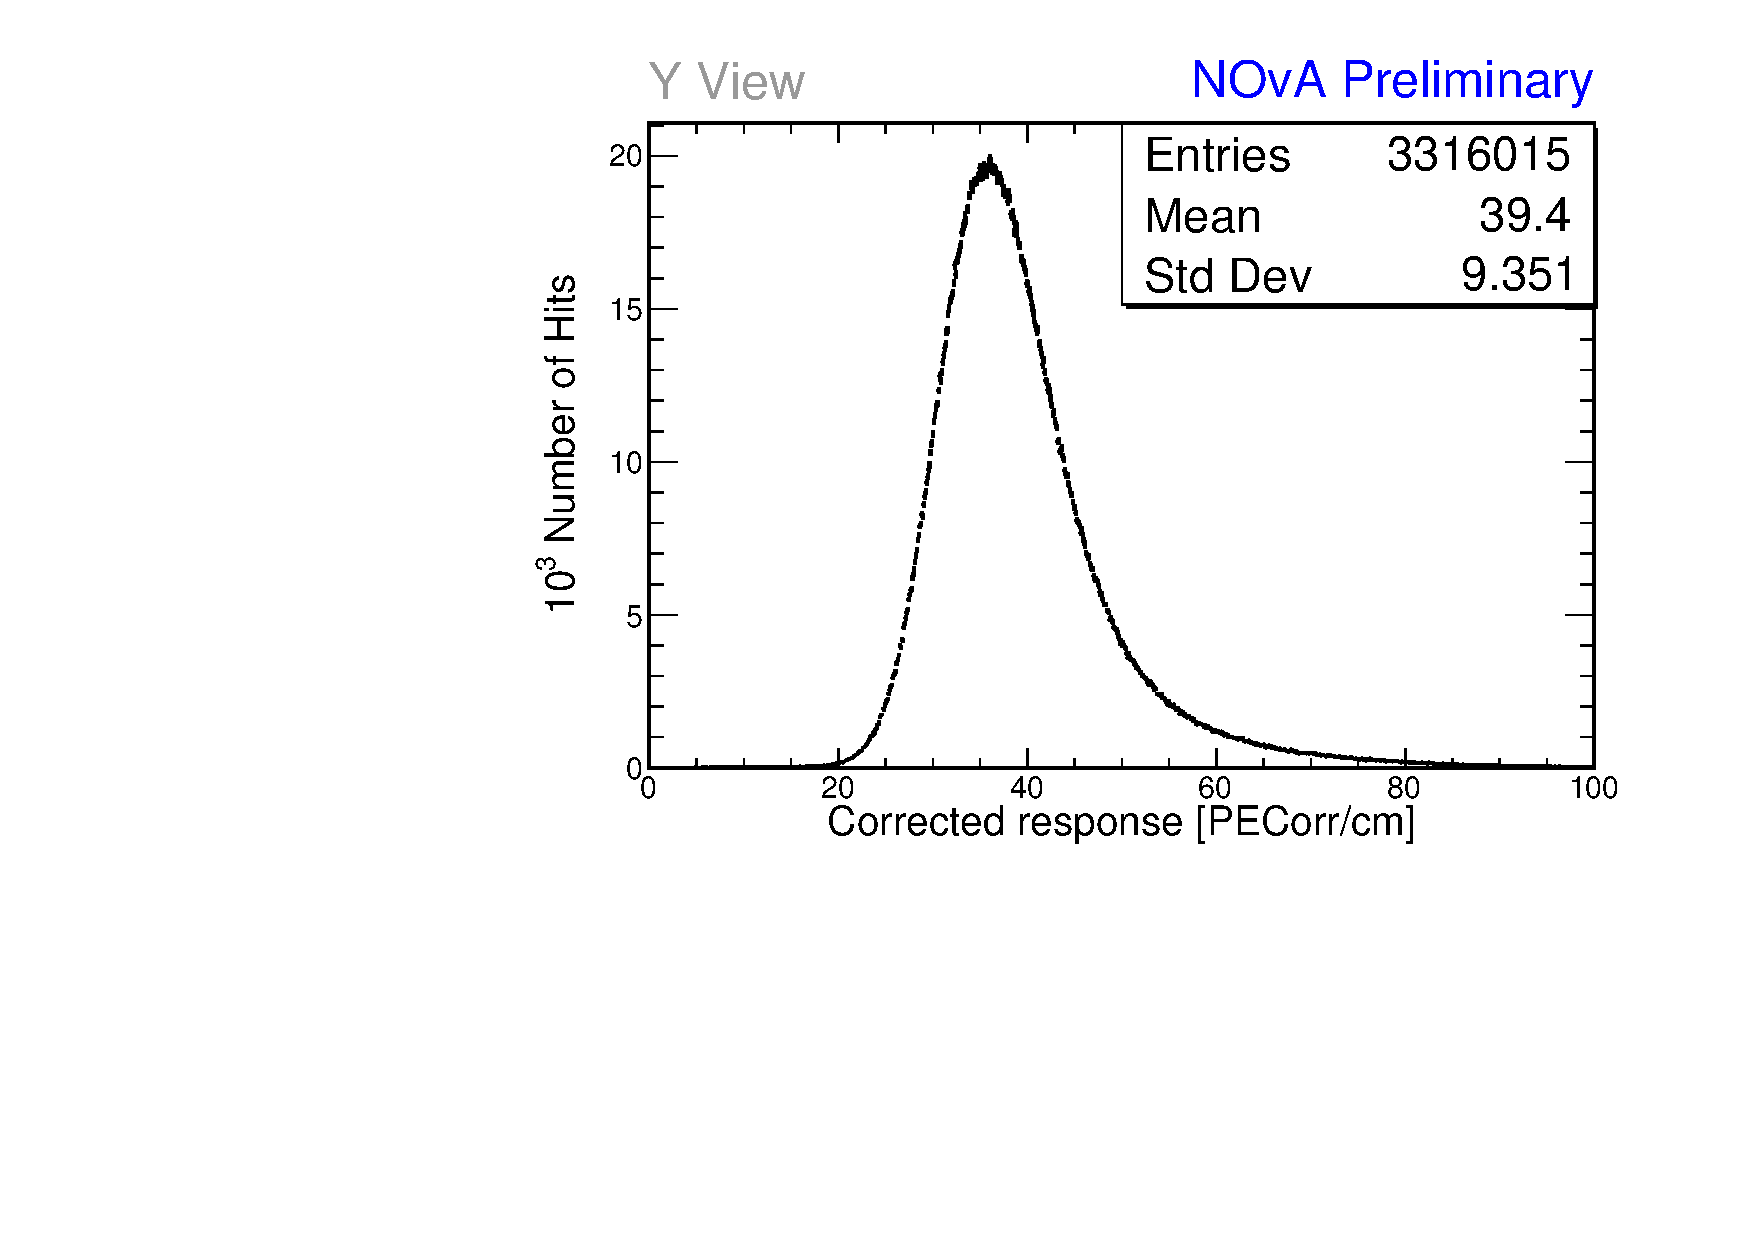
\includegraphics[width=0.49\textwidth]{Plots/NOvAExperiment/ExampleAbsCalib_P4_meu_y.pdf}
    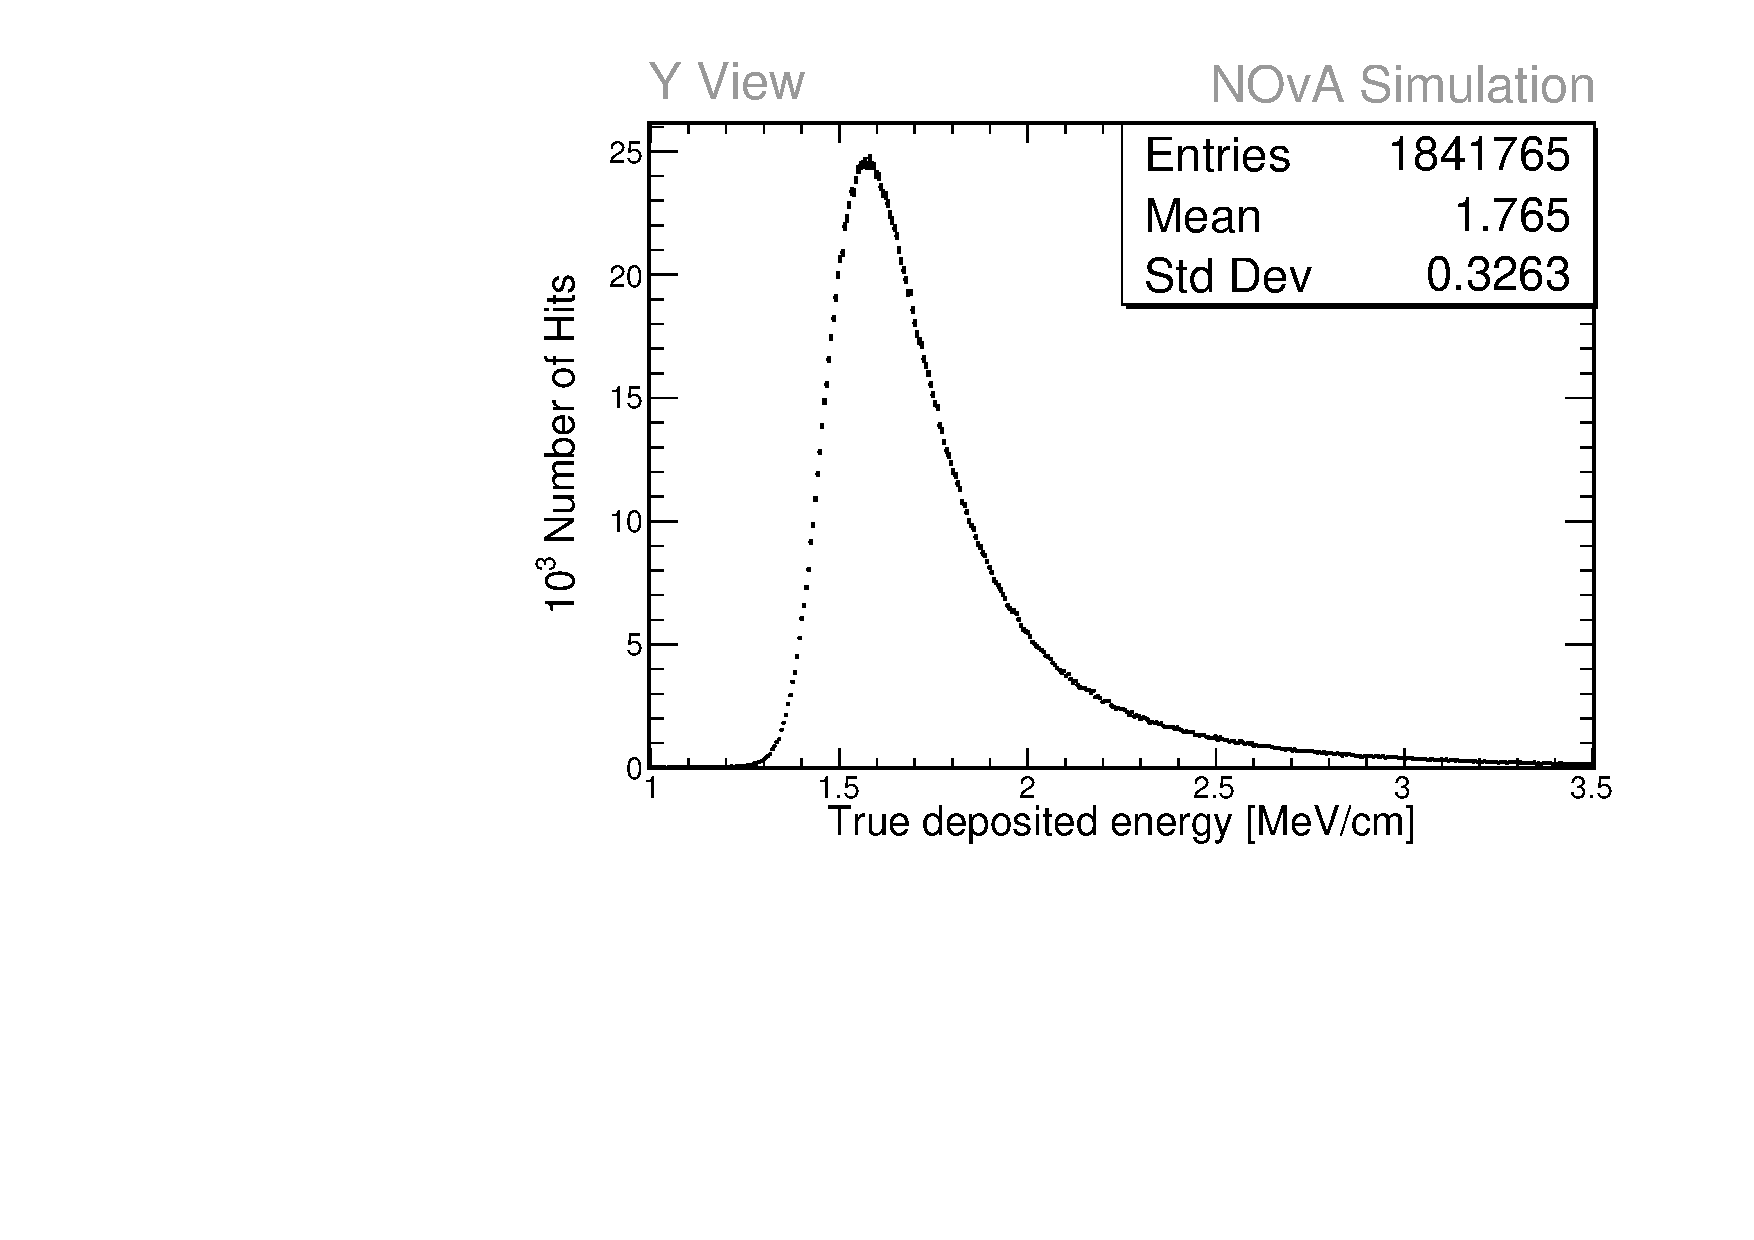
\includegraphics[width=0.49\textwidth]{Plots/NOvAExperiment/ExampleAbsCalib_Sim_mev_y.pdf}
    \caption[Example distributions for the NOvA absolute calibration]{To calculate the absolute energy scale we take the mean reconstructed energy response (left) for selected stopping muons for each view and each data period or simulation, and use it to divide the simulated mean true deposited energy (right).}
    \label{fig:NOvACalibrationAbsoluteEnergyScale}
\end{figure}

%For each calibrated data and simulation sample we take a mean of the corrected deposited energy distribution, separate for each view. We then take a simple average from the two views to get the final $\textsf{MEU}_{reco}$ in units of $\unit{PECorr/cm}$ for each sample \cite{NOvA-doc-13579-FACalorimetricEnergyScale}. Additionally, from simulation we can get the mean of the distribution of the true deposited energy in the scintillator, $\textsf{MEU}_{truth}$ in units of $\unit{MeV/cm}$ for the same sample of stopping muons. 

We save these absolute energy scales, as well as the results of the attenuation fit, in a set of lookup tables, which are used any time a hit is recorded in the \gls{NOvA} detector and processed through the \gls{NOvA} data processing algorithms.

%Stopping muons provide a good sample of known energy deposits. If we can collect a “golden” sample, they should provide the scale factor to convert PECorr to GeV. So far, the method used has been imperfect, and the absolute calibration constants are known to be off by approx. 10\%. Since a factor already has to be derived to correct for dead material, this is not significantly impeding current efforts, but work was recently gone into improving this area. [docdb:7410 - this was likely before the track window cut was introduced] (Here it says that it's not such a big a problem since we have to scale for the dead material anyway. But nowadays we have to account for a large systematic uncertainty in the absolute energy scale in our analyses. How is the dead material correction different from the energy scale uncertainty?)

%...the calibration of the calorimetric energy scale of the NOvA detectors uses the energy deposited by stopping muons as a standard candle. To reduce systematic uncertainties, only those energy deposits in a 1-2 m window away from the muon track end point are used. The mean of the detector response distribution is found for data and MC in both near and far detectors. The mean of the distribution of true energy deposits in the track window is used to provide a conversion factor between the detector response and the true energy deposited in the scintillator for minimum ionising muons. The simulated dE/dx is uniform within about 1.8\% for hits around the minimum between 100-200 cm from the track end. The energy that a muon deposits within each cell is estimated using Geant 4 and stored in Fibre Liquid Scintillator (FLS) hits. FLS hits are only those within the active material (liquid scintillator) and energy loss within the passive material (plastic extrusions) is ignored. an estimate of the minimum energy loss rate of stopping muons in the NOvA scintillator is found to be,
%\begin{equation}
%\left.\frac{dE}{dx}\right|_{\textsf{mip}}=\left(1.7915\pm 0.0035\right)\unit{MeV/cm}.
%\end{equation}
%For stopping muons in NOvA it is also important to consider their decay. The muon has a vacuum lifetime of about 2.2 microseconds and favourably decays, with a branching ratio approx. 100\%, into an electron, an electron anti-neutrino and a muon neutrino. The electron produced in this decay is called a Michel electron and is used to select muons that stop within the NOvA detectors. The energy scale calibration is performed using cosmic ray muons. The calibration measures the detector response in data and MC in both near and far detectors and normalises them all by providing a conversion factor, for all four cases, that converts the detector response to energy in GeV. The energy loss rate (dE/dx) of stopping muons is well described by the Bethe-Bloch and is a function of the distance from the stopping point. A track window technique is used to minimise the variations in detector response that depend on the distance to the track end. Using this technique only hits within a region of distances from the track end are used. The position of the track window is chosen such that a mis-reconstruction of the track end point has the minimum effect on the mean detector response. The track window is currently set to be in the range from 100 cm to 200 cm from the track end.[docdb:13579 - FA\_Calorimetric\_energy\_scale]

\section{Energy Estimation}\label{sec:NOvAEnergyEstimation}
The deposited energy we get from the detector calibration (Sec.~\ref{sec:NOvACalibration}) is only the first step in estimating the neutrino energy $\left(E_\nu\right)$ required for the main \gls{NOvA} analyses.

For the $\nu_\mu$ disappearance analysis, the $E_{\nu_\mu}$ is measured as the sum of the muon energy and the energy of the hadronic shower \cite{NOvAResults2021.pdf}. The energy of the muon is identified from the length of its track, without the need of the calibration results. The energy of the hadronic shower is estimated from simulation as a fit to the 2D distribution of the true $E_{\nu_\mu}$ minus the reconstructed muon energy, versus the visible (not corrected for the dead material) deposited energy of the hadronic system \cite{PsihasNOvAThesis_ProngCVN.pdf}.

For the $\nu_e$ appearance analysis, the $E_{\nu_e}$ is calculated using a quartic fit to the 2D distribution of the electromagnetic and the hadronic calorimetric energies corrected for energy deposition in the dead material (\gls{PVC} cells) \cite{PsihasNOvAThesis_ProngCVN.pdf}. The dead material correction is currently just a simple scaling of the deposited energy from calibration for all particles and it is calculated from the measurement of the $\pi^0$ mass peak in the \gls{NOvA} \gls{ND}. This correction is correct only for electromagnetic showers and is not directly applicable to hadronic showers. The fit to determine $E_{\nu_e}$ keeps the normalization of both the electromagnetic and the hadronic energies free, so the correctness of the dead material correction is not important. It is however used in other, non-neutrino oscillation analyses.

\section{Systematic Uncertainties at NOvA}\label{sec:NOvASystematics}

Systematic uncertainties in \gls{NOvA} analyses arise from the imperfect knowledge on the individual components of the \gls{NOvA} experiment, or from the known shortcomings of the prediction used to extract the results on the measured parameters. Even though different analysis in \gls{NOvA} need to consider different systematic uncertainties and their effect on the results varies, there are a few commonalities across all \gls{NOvA} analyses that are explained below.

Both the 3-flavour \cite{NOvAResults2021.pdf} and the sterile neutrino \cite{NOvASterilesFHCRHCResults2021.pdf} oscillation analyses in \gls{NOvA} use the \gls{ND} to constrain the \gls{FD} prediction, which significantly reduces the effect of the neutrino beam and interaction prediction systematic uncertainties. On the other hand, these are the leading sources of systematic uncertainties for the \gls{ND}-only analyses, such as the cross section analyses \cite{NOvANCPi0XSecMeasurement2019.pdf, NOvANumuCCXSexMeasurement2023.pdf, NOvANueCCXSecMeasurement2023.pdf, NOvANuMuCCPi0XSecMeasurement2023.pdf}. The leading systematic uncertainty for the neutrino oscillation measurements comes from the detector calibration uncertainty. Significant uncertainties for all NOvA measurements also come from the neutron modelling, the detector simulation and the muon energy estimation. There are other sources of systematic uncertainties that are not mentioned here as they are sub-dominant, or specific to a certain analysis.

The systematic uncertainty on the prediction of the neutrino beam consists of two parts: the hadron production and the beam focusing uncertainties \cite{NuMIFlux.pdf}. The uncertainty for hadron production is estimated by the \gls{PPFX} (describe in Sec.~\ref{sec:NOvASimulation}) using the multi-universe technique. Here we create 100 \gls{PPFX} universes in which the inputs from the external measurements used to constrain the hadron production are randomly floated around their central values within their respective systematic uncertainties. Parts of the hadron production that are not constrained by external measurements are given a conservatively large systematic uncertainty. The beam focusing systematic uncertainties account for the uncertainties on the horn and target positions, the horn current, the beam position on the target, the beam spot size, and the effect of Earth's magnetic field in the beam pipe. %Since all these uncertainties can be correlated between each other, especially for an off-axis detector such as in NOvA, we perform a \gls{PCA} to estimate the bin-to-bin covariances in true energy for each neutrino flavour, detector and beam mode. 
\todo{Describe the beam PCA and how can we limit the beam uncertainty}

%[NosekThesisNOvAOscillationSysts2021.pdf]

%From docdb:54582: NOvA analyses use two sets of flux uncertainties: beam transport, which cover differences between the simulation and the working conditions of the NuMI beam, and hadron production, which concern the rates of production of pions and kaons from proton collisions on the carbon target. The beam transport uncertainties include the horn and target position, the horn current, the beam position on the target, the beam spot size, and the effect of the Earth’s magnetic field in the beam pipe (which is not simulated in G4NuMI). The effect of each uncertainty is below 5% at the flux peak for both the ND and FD. PPFX is used to constraint the hadron production models for the NuMI beam using external hadron production data and theory. The systematic effect is assessed by generating 100 universes where the uncertainty on the external data and theoretical assumptions are allowed to float. Flux uncertainties are known to show correlations across most neutrino energy bins, especially in off-axis measurements like NOvA. NOvA looks at 100 PPFX universes, and for each PPFX universe we further sample the beam transport parameters 20 times, creating a total of 2000 universes representing many different possibilities of the flux uncertainty. These universes are used to estimate the bin-to-bin covariances in true energy for each neutrino flavour, detector and beam mode. A Principal Component Analysis (PCA) is applied to the covariance matrices to find sets of uncorrelated shifts - Principal Components (PCs). The covariance matrices for each neutrino flavour and beam mode are calculated in the (ND, FD/ND) basis to represent the approximate extrapolated error at the Far Detector. These are then diagonalized to give the Principal Components, given by the eigenvectors i.e, $PC_i=\sqrt{\lambda_i}v_i$, where $\lambda_i$ represents the $i$-th largest eigenvalue and $v_i$ its corresponding eigenvector. The components are then converted to the (ND, FD) basis. Each PC can be used as a systematic shift in the oscillation fit with a pull of $1\sigma$. By ordering each of the PCs in terms of the magnitude of their eigenvalues, one can also capture most of the information embedded in the covariance matrix with just a few components. Five principal components are used in the oscillation fit. The hadron production uncertainty on the neutrino flux is evaluated using a "multi-universe" technique. This is $\sim 7\%$ at the spectrum peak dominated by interactions where relevant data to be included in the constraining procedure is currently not available (mostly mesons and proton quasi-elastic interactions). Beam transport uncertainties are incorporated by propagating uncertainties in the alignment of beamline elements, including the beam position on the target, the horns current and position, the beam spot size, and the effect of the Earth magnetic field in the decay pipe. The beam optic uncertainty is $\sim 4\%$ at the peak.

%Not sure if I should include a discussion on nu-on-e, or low nu studies here, or just PPFX improvements.

%%% Neutrino interaction systematic uncertainties
\todo{Describe the neutrino interaction modelling systematic uncertainties}
%[NOvAResults2021.pdf] Neutrino interaction model uncertainties are evaluated using the event reweighting framework in GENIE with additional uncertainties constructed by NOvA as follows. Uncertainties on CCQE RPA, low-Q2 RES suppression, 2p2h, and nonresonant and incoherent N$\pi$ production are established for the new model set using methods similar to those in Ref. [84]. Pion FSI uncertainties are based on comparisons to πþ on 12 C scattering data [66–72] and prior studies using an alternative neutrino interaction generator [85]. Uncertainties on the nue(anu) CC cross section relative to the numu(anumu) CC cross section due to radiative corrections and possible second-class currents are unchanged from previous analyses [83].

%[NOvAResultsNuOnly2018.pdf] Estimates for the majority of the cross section and FSI uncertainties that we consider are obtained using the event reweighting framework in GENIE [15]. However, ongoing effort in the neutrino cross section community and the NOvA ND data suggest some modifications are necessary. First, we apply additional uncertainty to the energy- and momentum-transfer dependence of CC quasielastic (CCQE) scattering due to long-range nuclear correlations [44] according to the prescription in Ref. [21]. Second, as the detailed nature of MEC interactions is not well understood, we construct uncertainties for the neutrino energy dependence, energy-transfer dependence, and final-state nucleon-nucleon pair composition based on a survey of available theoretical treatments [45–47]. The normalization of the MEC component is recomputed under each of these uncertainties using the same fit procedure used to arrive at the 20\% scale factor for the central value prediction. Third, it is now believed that the inflated value of the axial mass in quasielastic scattering (M QE A ) obtained in recent neutrino-nucleus scattering experiments relative to the light liquid bubble chamber measurements is due to nuclear effects [48] that we are now treating explicitly with the foregoing. We thus reduce GENIE’s uncertainty for M QE A to pm5\% (a conservative estimate of the bubble chamber range [49,50]) from its default of +25\% −15\%, while retaining GENIE’s central value M QE A = 0.99 GeVc2. Fourth, we increase the uncertainty applied to nonresonant pion production with three or more pions and invariant hadronic mass of W < 3 GeV to 50% to match the default for one- and two-pion cases, based on data-simulation disagreements observed in the ND data. Fifth, and finally, we introduce two separate 2% uncertainties on the ratio of nueCC and numuCC cross sections: one to account for potential differences between them due to radiative corrections and one to consider the possibility of second-class currents in CCQE events [7,51]. To validate the uncertainties assigned by GENIE to the NC backgrounds in our analyses, we performed a study within the numuCC candidate sample in the ND that measured the rates of neutrons that were produced at the ends of tracks and subsequently recaptured, emitting photons. This study was done by investigating time-delayed activity consistent with a neutron capture, taking into account the tail of the Michel electron time spectrum. The neutron rate is different for the mostly mu- identified in numuCC reactions versus the mostly pi+- in NC. This study suggested that the NC cross section uncertainties provided by GENIE, combined together with the calibration uncertainties mentioned previously, account for any differences between data and simulation. Therefore, we no longer include the ad hoc 100\% additional uncertainty on NC backgrounds used in previous results [5,16].

%%% Detector modelling
\todo{Describe the detector modelling systematic uncertainties}
\note{I should probably only discuss the new light level and cherenkov systematic uncertainties from the 3fl technote. This have not been published anywhere yet, but this is what I'm using for the mag. moment analysis}
%[NOvAResults2021.pdf] Uncertainties arising from the custom light model are assigned based on comparison to a more robust response model that was not fully incorporated into the simulation for this analysis. This model is constrained by a sample of ND proton candidates in addition to the muon sample used previously. Differences in the detector response between the proton and muon samples also provide a data-driven uncertainty on the relative production of Cherenkov and scintillation light in the model.

% I should probably just quote this uncertainty from the 3 flavour technote and say that it has been changed and improved since the last published analysis - or no? this is the uncertainty I'm going to be using so probably...

%%% Neutron modelling?
\todo{Describe the neutron uncertainty - why do we need it?}
\note{Should I describe MENATE or MCNP? Do I even need this here? Not sure if I'm including this in the mag. moment yet. Maybe add it only if I do...}

%%% Calibration scale, shape and ageing systematic uncertainty
\todo{Describe the calibration uncertainties}
%[NOvAResults2021.pdf] Detector calibration uncertainties remain dominant and are driven by a 5\% uncertainty in the calorimetric energy scale. Additionally, a new time-dependent calibration uncertainty is included to account for any residual differences remaining after performing the calibration over shorter time periods as mentioned previously.

%[NOvAResultsNuOnly2018.pdf] The overall energy response uncertainty, on the other hand, is driven by uncertainty in our overall calorimetric energy calibration. To investigate the response, we compare simulated and measured data distributions of numerous channels including the energy deposits of muons originating from cosmogenic- and beam-related activity, the energy spectra of electrons arising from the decay of stopped muons, the invariant mass spectrum of neutral pion decays into photons, and the proton energy scales in ND quasielasticlike events. The uncertainty we use is guided by the channel exhibiting the largest differences, the proton energy scale, at 5\%. We take this 5\% uncertainty as both an absolute energy uncertainty, correlated between the two detectors, and a separate 5\% relative uncertainty, since there are not sufficient quasielasticlike events to perform this check at the FD

%First Analysis systematic uncertainties due to calibration:
%Sources of systematic uncertainty of particular concern are those introduced by residual variations remaining after calibration. Systematic errors are introduced by spatial and temporal variations in detector response. Further, any difference between the two detectors may introduce a relative shift in the energy scale between the detectors. A source of systematic uncertainty can be introduced by mis-reconstructing the end point of the muon track. Such a mis-reconstruction would shift the window within which hits are selected and hence the dE/dx of the muon.  The figure shows that the detector response varies by up to about 60\% over the range from 0 to 500 cm to the track end. This large variation illustrates the importance of careful consideration of the track window position and size. The detector response for both data and MC is minimum at about 130 cm from the track end and is flat to about 1\% in the range from 100 cm to 200 cm from the track end. For a track window starting at 100 cm from the track end, a conservative mis-reconstruction of the track end point by 10cm will shift the start of the track window to between 90cm and 110cm. This shift will alter the MEU value by less than 0.4\% over the range.
%If the calibration procedure was ideal the detector response would not vary with position in either data or MC. The calibration is not ideal and the detector response and recorded simulated energy deposition varies with position of the hit within the detector, such variations will introduce systematic errors. The position of a hit can be defined by the plane, cell within the plane, and distance along the cell (w) of the hit. The variation in detector response and simulated energy deposition vs. plane, cell and w for each view has been studied to quantify the systematic uncertainty introduced by these sources.
%The rise in detector response at the far end of FD y-view cells is an issue with several potential sources. The rise in response may be due to an acceptance effect or a light-level threshold effect among other possibilities. An acceptance effect is where greater energy must be deposited at the far end of the cells so that the light can travel along the fibre, hit the APD and be recorded as a hit. Both an acceptance effect and a light-level effect would introduce a bias towards higher energy hits toward the far end of cells.
%Another source of systematic uncertainty is introduced by the variation in detector response with time. The FD response is stable to about 1\% during the period from October 2014 to March 2015. The ND response needs further study but there was no significant trend over 6 months at 5\%. 
%As mentioned in Section 5, the version (7.1) of the calibration used for first analysis has been adjusted based on studies of muons from beam neutrinos interacting in the detector [8]. A shift of 3.6\% was introduced based on the average response of muons where large sections of the track were used. When only a track window of 100-200cm is used on the beam muons the difference is only 2.7\% [8]. Our best hypothesis for this residual 2.7\% difference is that it is caused by showery events that are present in ND data but not ND MC: it was shown in [9] that doing the calorimetric energy scale calibration using a truncated mean (or a median or a fit to the peak) gave a data/MC ratio that differed by 2.7\% compared to using the untruncated mean as described in this document. A comparison of various cross checks of the calorimetric energy scale was undertaken (in [10] and [11]) and concluded that the nearly 5\% difference between ND data and MC seen in a sample of Michele electrons [12] should be applied as both an absolute and relative shift to the calorimetric energy scale. The difference between the level of calorimetric energy resolution of stopping muons was studied and it was found that data and MC agreed best when an 8\% additional smearing was introduced. Studies for the NuMu analysis indicated that this was a negligible systematic uncertainty [13]. 
%[docdb:13579 - FA\_Calorimetric\_energy\_scale]

%%% Muon energy scale - is this necessary?
\todo{Describe the muon energy scale uncertainty - if needed, maybe just briefly...}
%\chapter{NOvA Test Beam Detector Calibration}\label{sec:TestBeamCalibration}

The \gls{NOvA} Test Beam experiment~\cite{NOvATestBeamWallbangProceedings2020.pdf} is a sub-experiment designed to enhance \gls{NOvA}'s sensitivity to neutrino oscillation measurements by improving the understanding of particle interactions and energy deposition within the \gls{NOvA} detectors. Initial studies~\cite{NOvA-doc-33012} showed that, only by improving the detector calibration, the Test Beam experiment has the potential to reduce the total systematic uncertainty in the measurement of the three flavour oscillation parameters by about 10\%.
 
The \gls{NOvA} Test Beam experiment consists of a scaled down version of the \gls{NOvA} detectors placed in a test beam. Using a test beam allows for the study of the response of tagged single particles with known momenta and positions within a \gls{NOvA} detector. Additionally, this setup enables the determination of the energy resolution and the absolute energy scale without the use of simulation. Furthermore, it permits the comparison of responses between beam muons and cosmic ray muons, study of fibre attenuation, and validation of the \gls{NOvA} calibration process. The Test Beam detector is equipped with a combination of the \gls{ND} and \gls{FD} readout electronics and filled with a range of \gls{NOvA} scintillator oils, enabling a comparison of their respective performance and particle responses \cite{NOvA-doc-15750}. All these advantages require, or benefit from, the calibration of the Test Beam detector, which follows the same calibration procedure as the standard \gls{NOvA} detectors (Sec.~\ref{sec:NOvACalibration}).

In this chapter I introduce the \gls{NOvA} Test Beam experiment in Sec.~\ref{sec:TBExperiment}, focusing on the Test Beam detector and especially on the aspects that could impact its calibration. Section~\ref{sec:DataBasedSimulation} describes the new data-based simulation of cosmic muons that I developed for the Test Beam detector calibration, while Sec.~\ref{sec:TBCalibrationSection} discusses the calibration of the Test Beam detector itself.
%Here we present the differences from the calibration of the \gls{NOvA} \gls{ND} and \gls{FD}, as well as the results and their discussion and validation.

%Only considering improvement in the calibration systematic uncertainty, the NOvA Test Beam program can reduce the overal systematic uncertainty for the main NOvA measurements by about 10\% [docdb:33012] (talk also contains a list of other talks on impact of TB in different NOvA areas). For DeltaM2: By increasing exposure, total syst. error decreases by (+) 18.5% (-) 25%; By increasing exposure and reducing calib systs., total syst. error decreases by: (+) 26% (-) 32%; Difference between the above (reducing calib systs. with large exposure): (+) 9.6% (-) 9.4%. For sin2Th23: Difference by reducing calib syst.: (+) 10.8% (-) 9.4%.
%Statement: “The NOvA Test Beam will improve the total systema6c error on the final measurement of the oscilla6on parameters Dm232 and sin2Th23 by 10% from reduc6on of calibra6on systema6cs alone. Further, NOvA analyses will benefit from the detailed understanding of detector response to hadronic, electromagne6c, and muon energy provided by the Test Beam, which will be essen6al to solidify understanding of systema6cs, uncover poten6ally new uncertain6es, tune the simula6on modeling, and improve reconstruc6on and PID algorithms.”
%Potential Test Beam impacts: Check modeling of hadronic interacOons in detector (check GEANT systemaOcs), Using Test Beam data as “single-parOcle MC” to train CVN prong-like algorithms, GeneraOve Adversarial Networks for MC improvements using Test Beam data, Check ND calibraOon procedure to try and understand causes of 3-5% discrepancy between data and MC for muons and protons  (Birks suppression measurement), Data/MC comparisons of observed and clustered visible energy to improve dead material correcOons and energy esOmators, Acquire beier understanding of gain and photon transport, aienuaOon, Cherenkov light modeling, [DifferenOal] charged pion and proton cross secOon measurements would be extremely useful!, CalibraOng with test beam muons vs. cosmic muons (differences between horizontal vs. verOcal muons? - possibly shed “light” on the calib shape uncertainty), Study path length inside cell, take beam data with non-orthogonal incidence, Cross-check pi0 invariant mass reconstrucOon and Michel tagging efficiency/spectra, Use neutron source to study modeling of neutron capture (I don't think this was done in the end...), Playing with different GEANT physics lists to boost our confidence in the MC (pions? neutrons?)

%[docdb:15750 - NOvA Test Beam task force report]: The test beam program was included in the NOvA proposal [1] and was considered as an essential part of the experiment since its inception. Primary goals are oriented toward measurements of detector response to different particles with a range of momenta most relevant to NOvA beam physics studies, establishing of the absolute and relative energy scale of both NOvA detectors, and validating detailed and fast detector simulations code. [List all possible desired studies with Test Beam copied below] Two 31-layer 2 × 2 blocks, with approximate dimensions of 2.6 × 2.6 × 4 m3 were produced at the Minnesota factory before its shutdown (as a comparison, the 3 × 3 NOvA ND has 6 × 32 layers). In addition, 96 1 × 1 layers, with approximate total dimensions of 1.3 × 1.3 × 6.2 m3 were produced. Both 2 × 2 blocks and all the 1 × 1 layers were leak-tested. The 2 × 2 blocks are currently stored at the MINOS surface building, while the 1 × 1 layers are stored at the CDF building(?). The proposed detector to be deployed for the test beam run consists of the two 2 × 2 blocks. The NDOS decommissioning yielded 25000 gallons of scintillator. Since storage available is limited to 12000 gallons, it was decided to blend most of the 5000 gallons of existing ND/FD scintillator with the NDOS scintillator. 200 gallons of ND/FD scintillator, which has a slightly higher photon yield, are reserved for special studies. We also plan to reuse the NDOS secondary containment tub to provide oil+scintillator containment in case the test beam detector undergoes a catastrophic structural failure. Based on MINERvA’s experience, it is anticipated that two months of data taking would provide the necessary samples to carry out the test beam objectives.

%Also use information from:
%\begin{itemize}
%\item NOvA Test Beam Technical Statement of Work
%\item NOvA Test Beam program (paper for DOE) [docdb:25074]
%\item NOvA Test Beam task force report [docdb:15750]
%\item Overview presentation of NOvA Test Beam [docdb:20495]
%\item Test Beam support document [docdb:22172]
%\item NOvA Test Beam program proceedings [docdb:55808]
%\end{itemize}

%%%%%%%%%%%%%%%%%%%%%%%%%%%%%%%%%%%%%%%%%%%%%%%%%%%%%%%%%%%%%%%%%%%%%%%%%%%%%%%
%%%%%%%%%%%%%%%%%%%%%%%%%%%%%%%%%%%%%%%%%%%%%%%%%%%%%%%%%%%%%%%%%%%%%%%%%%%%%%%
%%%
%%%                       Test Beam detector description
%%%
%%%%%%%%%%%%%%%%%%%%%%%%%%%%%%%%%%%%%%%%%%%%%%%%%%%%%%%%%%%%%%%%%%%%%%%%%%%%%%%
\section{The NOvA Test Beam Experiment}\label{sec:TBExperiment}
%What is Test Beam, how does the detector and beamline look like.
%Placed in MC7b together with a beamline instrumentation (no need to describe beamline).

The \gls{NOvA} Test Beam experiment~\cite{NOvA-doc-22172} consists of a scaled down version of the \gls{NOvA} \gls{ND} and \gls{FD}, shown in Fig.~\ref{fig:TBDetector}, and a series of beamline detectors to measure and identify a range of particles from the MCenter beamline in the \gls{FTBF}~\cite{FTBFWebsite}.

\begin{figure}[!ht]
\centering
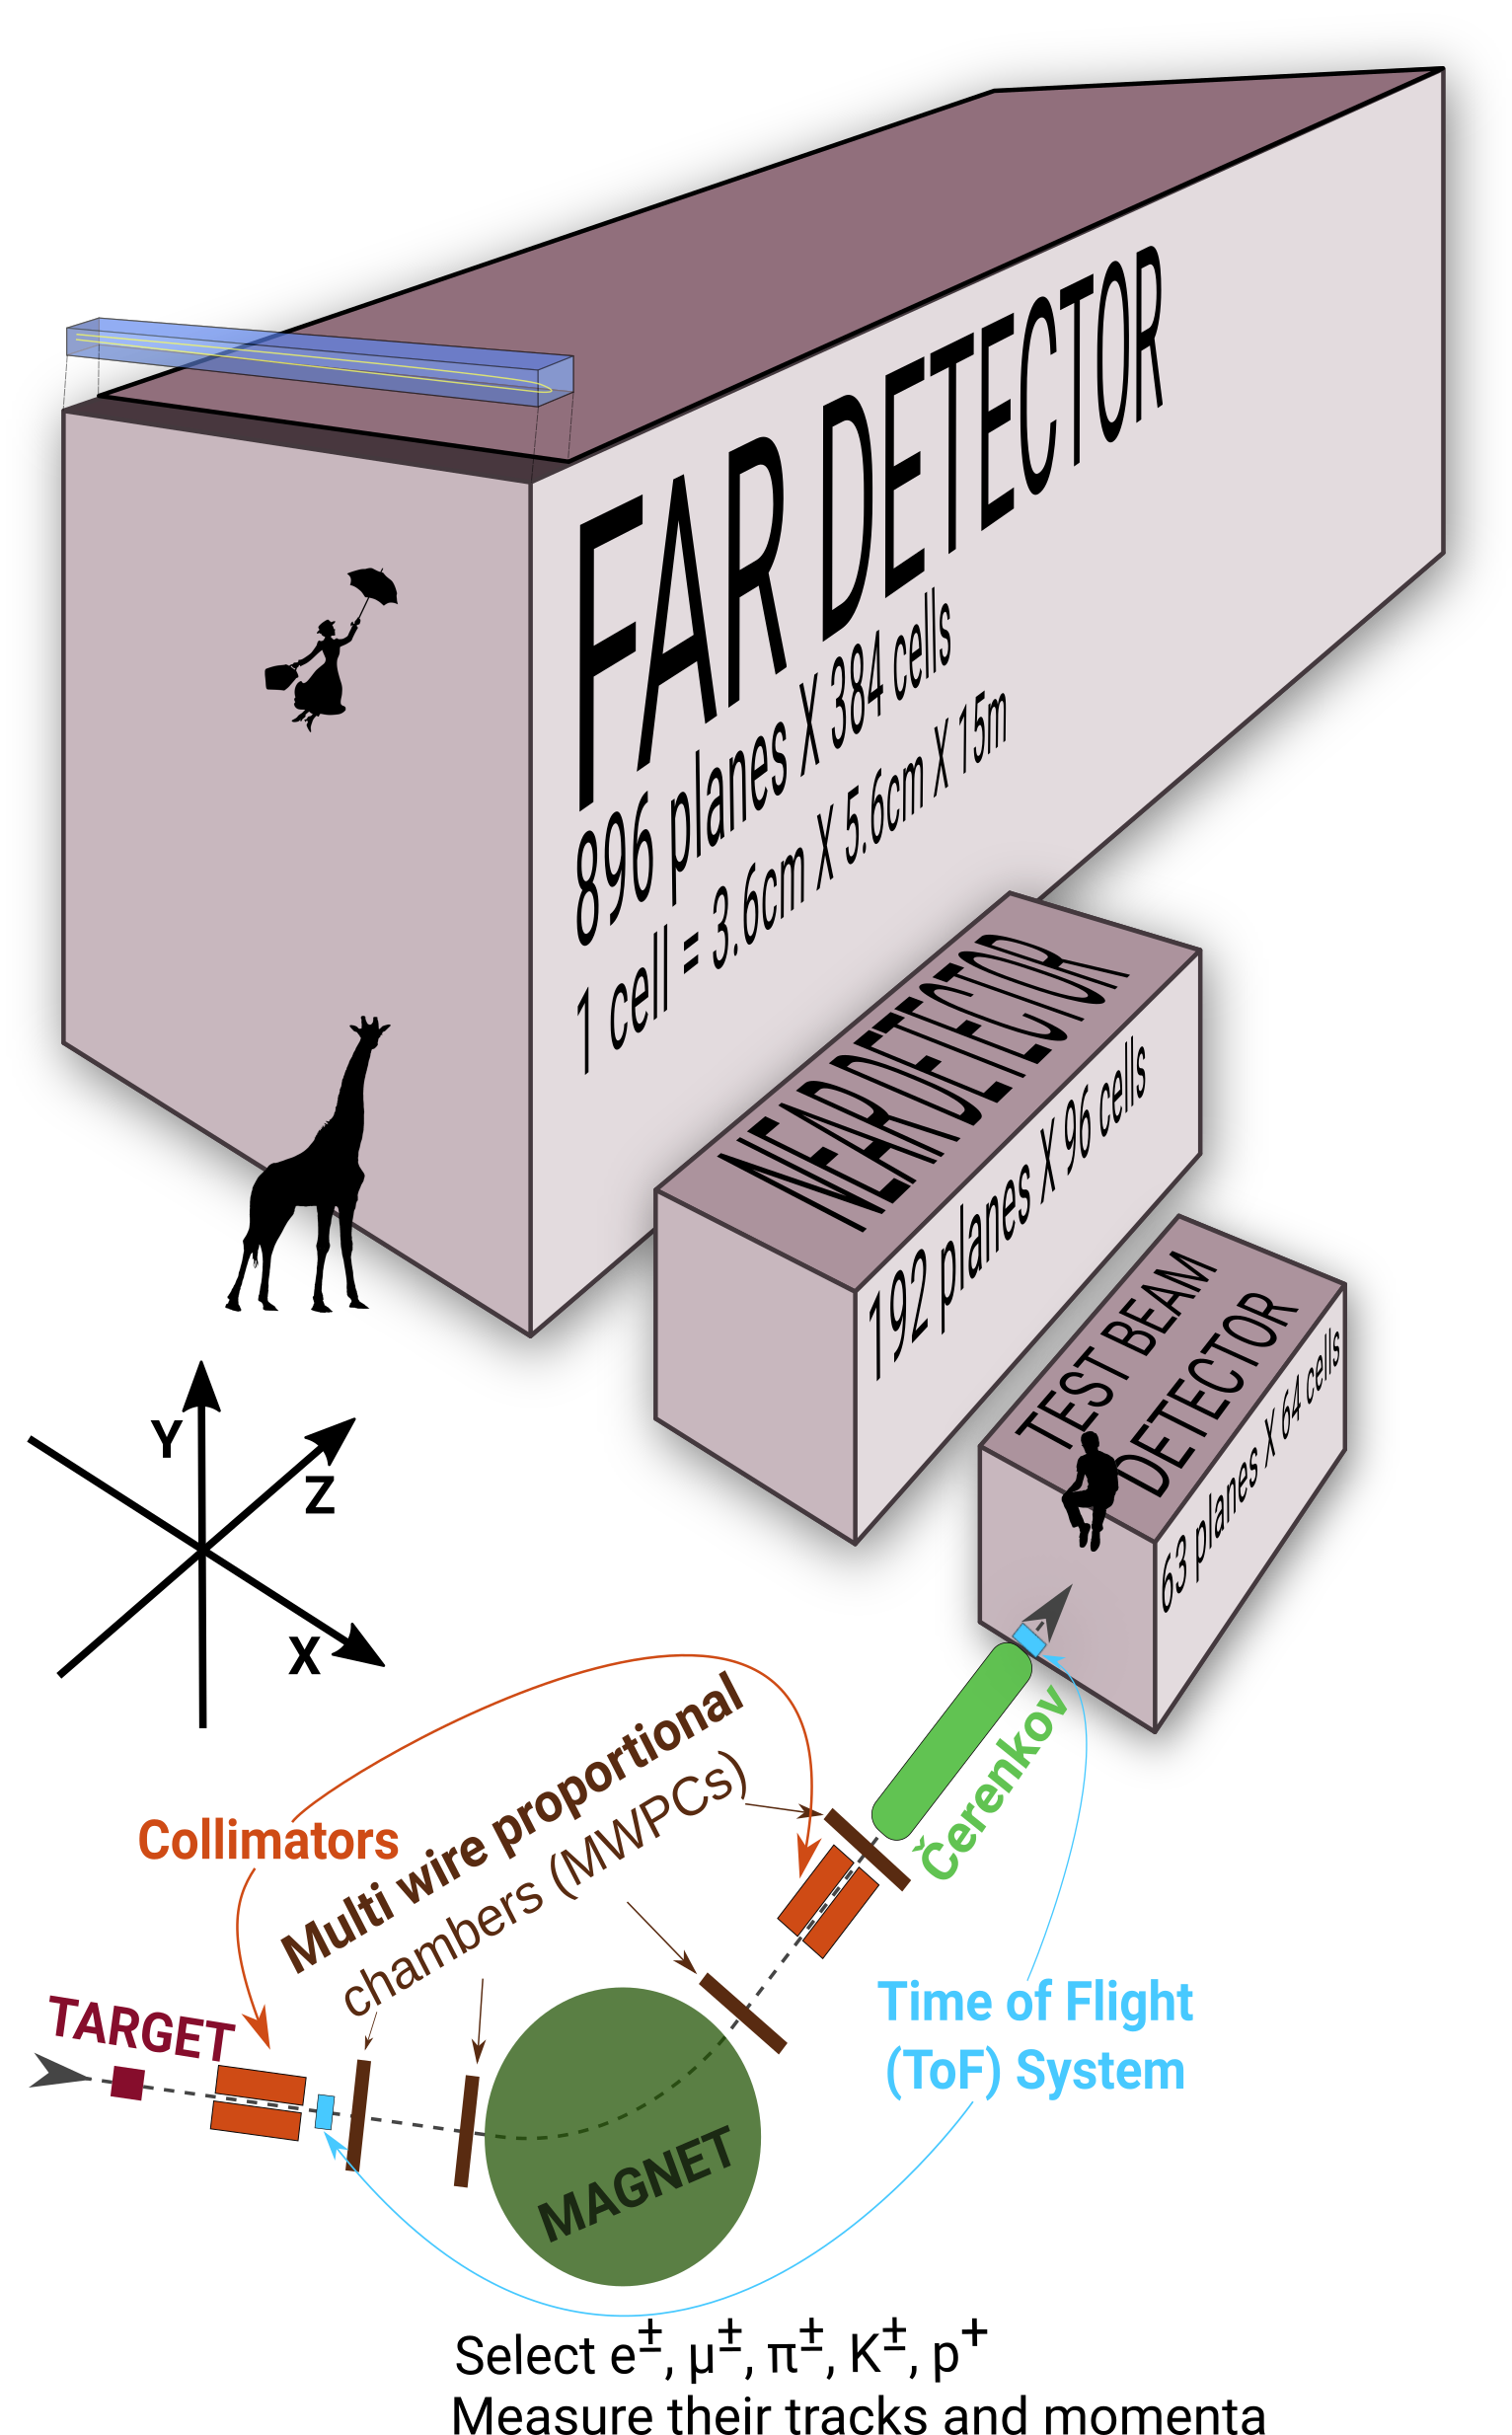
\includegraphics[width=.7\textwidth]{Plots/TBCalibration/TestBeamDetectorWithArrows.png}
\caption[Comparison of Test Beam detector to the Near and Far Detectors]{Comparison of Test Beam detector scale to the \acrshort{NOvA} \acrshort{ND} and \acrshort{FD} (and a man, giraffe, or Mary Poppins). Also shown are the Test Beam beamline detectors and components (not to scale), with arrows showing the direction of the beam. The three black arrows show the orientation of the detector coordinate system.}
\label{fig:TBDetector}
\end{figure}

%Should I aslo talk about the beam halo? Could that have an influence on the calibration? Maybe it's the peaks in the cosz distribution?

The operation of the Test Beam detector started with commissioning runs in June 2019 and ran, with an exception of regular summer shutdowns, until July 2022, after which it was decommissioned. The Test Beam data taking is divided into \textit{periods}, which are defined in Tab.~\ref{tab:TestBeamPeriods}. Period 1 only lasted for about a month and with only a half-filled detector, as explained below. It was therefore only used for detector commissioning and will not be used in any of the Test Beam physics analysis, or in the calibration.
\begin{table}[!ht]
\centering
\caption{Test Beam detector data taking periods.}
\def\arraystretch{1.4}
\begin{tabular}{l@{\hskip 1in}lcl}
Period 1 & June $3^{\textsf{rd}}$ 2019 & - & July $6^{\textsf{th}}$ 2019\\
Period 2 & December $5^{\textsf{th}}$ 2019 & - & March $20^{\textsf{th}}$ 2020\\
Period 3 & January $12^{\textsf{th}}$ 2021 & - & June $27^{\textsf{th}}$ 2021\\
Period 4 & November $30^{\textsf{th}}$ 2021 & - & July $10^{\textsf{th}}$ 2022
\end{tabular}
\label{tab:TestBeamPeriods}
\end{table}

Majority of the Test Beam detector and its instrumentation is identical to the other \gls{NOvA} detectors, with a few exceptions that could have an impact on the calibration. We are going to identify and discuss these differences in this section.

%[docdb:15750 - NOvA Test Beam task force report]: The test beam program was included in the NOvA proposal [1] and was considered as an essential part of the experiment since its inception. The main tangible result of these initial plans and later discussions was a production of special small extrusion modules, made at the end of the modules production stage, as possible components of a future test beam detector. In fact, this production followed and was based on initial simulations of a possible test beam experiment [5].

\subsubsection*{Beamline}
The beam for the Test Beam experiment originates from the same $\unit[120]{GeV}$ Main Injector protons used in \gls{NuMI}, extracted once a minute in a continuous $\unit[4.2]{s}$ spill~\cite{NOvATestBeamWallbangProceedings2020.pdf}. The protons are impinged on a copper target producing mostly protons and pions, which are then directed towards a second target, producing the tertiary beam of particles used in the Test Beam detector. As can be seen in Fig.~\ref{fig:TBDetector}, two collimators are used to direct the tertiary beam and a magnet to select the desired momentum. Particle tracking is done using the four \glspl{MWPC} and particle identification is done with a combination of \gls{ToF} detectors and a Cherenkov detector set for electron detection.

\subsubsection*{Detector Parameters}
The \gls{NOvA} Test Beam detector consists of two 31-plane blocks, each beginning and ending with a vertical plane, with an additional horizontal plane glued in-between them to preserve the alternating pattern \cite{NOvA-doc-29543}. Each plane consists of 2 modules side-by-side, both made up of 32 cells. Each cell is $2.6\,\unit{m}$ long with an inner (without the PVC) depth and width of $5.9\,\unit{cm}$ and $3.8\,\unit{cm}$ respectively, same as for the other \gls{NOvA} detectors. This brings the final dimensions of the Test Beam detector to 63 planes $\times$ 64 cells, or $2.6\times 2.6\times 4.1\,\unit{m^3}$.

The 63 planes are numbered from 0 to 62, with even numbers corresponding to vertical planes and odd numbers to horizontal planes. Cells are numbered 0 to 63, going from bottom to top for horizontal planes and left to right, when facing the front of the detector, for vertical planes.

The detector coordinate system is illustrated in Fig.~\ref{fig:TBDetector}. It is centred with $\left(0,0,0\right)$ in the centre of the first plane \cite{NOvA-doc-58388}. The x axis runs left to right when facing the front of the detector, y axis from bottom to top, and z axis goes along the beam direction from front to the back of the detector. Position within each cell ($w$) is aligned with the x (y) axis for the horizontal (vertical) cells, with $w=0$ centred in the middle of each cell. The exact geometry of the Test Beam detector was measured in several alignment surveys and is saved in gdml files \cite{NOvA-doc-57955}.

In the past we encountered an issue when trying to align the Test Beam detector with the beamline measurements by rotating the detector. This broke several assumptions within the Test Beam geometry \cite{NOvA-doc-58388} and manifested as uncalibrated cells in the back of the detector \cite{NOvA-doc-57516}. This was fixed by realigning both the detector and the beamline separately, based on the last alignment survey, measured during the decommissioning of the detector.

%FD: maxPlane=900, maxCell=390. ND: maxPlane=220, maxCell=100. TB: maxPlane=63, maxCell=64

\subsubsection*{Scintillator}
%[TB task force report]: The NDOS decommissioning yielded 25000 gallons of scintillator. Since storage available is limited to 12000 gallons, it was decided to blend most of the 5000 gallons of existing ND/FD scintillator with the NDOS scintillator. 200 gallons of ND/FD scintillator, which has a slightly higher photon yield, are reserved for special studies. We also plan to reuse the NDOS secondary containment tub to provide oil+scintillator containment in case the test beam detector undergoes a catastrophic structural failure.

Test Beam used a combination of the leftover \gls{ND} and \gls
{FD} production scintillator oils and the oil drained from the \gls{NOvA} \gls{NDOS} test detector. The used scintillator oils also differ in the way they were stored since the \gls{ND} and \gls{FD} filling, or the \gls{NDOS} draining, which apparently impacted its quality. These factors have a significant effect on the energy deposition within them. The distribution of individual scintillator oils and the relative difference in their energy response can be seen in Fig.~\ref{fig:Scintillators}.

%The Test Beam detector is filled with several different versions of the NOvA scintillator oil, which differ mainly in the way they were stored since the filling of the near and far detectors. This is illustrated on figure \ref{figScintillators}.

\begin{figure}[!ht]
\centering
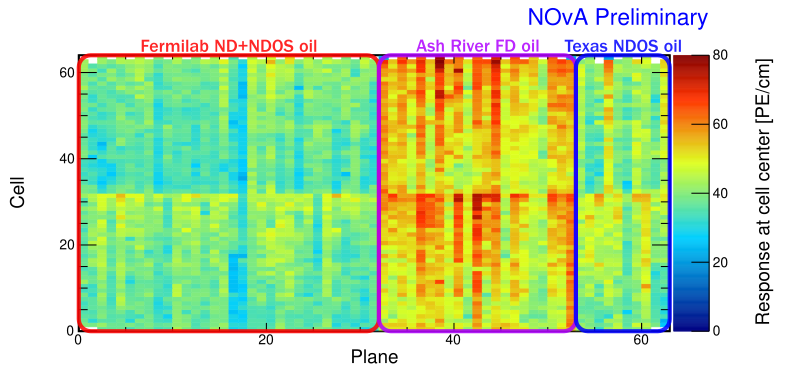
\includegraphics[width=\textwidth]{Plots/TBCalibration/TestBeamScintillatorOils.png}
\caption[Scintillator oils used in the Test Beam detector]{Uncorrected energy response in the centre of cells across the Test Beam detector showing a clear distinction between different scintillator oils, labelled with coloured boxes and descriptions.}
\label{fig:Scintillators}
\end{figure}

There are four distinct samples of \gls{NOvA} scintillator oil used in the Test Beam detector:
\begin{enumerate}
\item Mixed \gls{ND} production oil and \gls{NDOS}-drained oil stored in a tanker and four tanks outside in \gls{Fermilab} \cite{NOvA-doc-38349};
\item Separate \gls{ND} production oil and \gls{NDOS}-drained oil stored underground in barells at the MiniBooNE\footnote{MiniBooNE~\cite{MiniBooNEWebsite} is a \gls{Fermilab} experiment located close to the \gls{NOvA} \gls{ND}} cavern \cite{NOvA-doc-33012};
\item \gls{FD} production oil stored inside in Ash River in `totes' under several layers of black plastic \cite{NOvA-doc-34067};
\item \gls{NDOS}-drained oil stored mainly inside at Texas A\&M University and University of Texas at Austin \cite{NOvA-doc-38740, NOvA-doc-39088}.
\end{enumerate}

%The original plan \cite{NOVA-doc-34196} was to use the tanker and tank scinitillator for the entire Test Beam detector. However, due to extreme cloudeness of the scintillaotr in the tanks 

The original plan \cite{NOvA-doc-34196} was to only use the tanker/tank scintillator (sample \#1). First tests showed acceptable results and the tanker oil was used to fill out almost the entirety of the first block of the detector (first 32 planes) \cite{NOvA-doc-38349}. However, when the oil from tank \#2 was loaded into the tanker, it became extremely cloudy and unusable, possibly due to contamination with water accumulated at the bottom of the tanks. The rest of the first block was therefore topped up with high quality scintillator from \gls{NDOS} (sample \#2). This is labelled as `\gls{Fermilab} \gls{ND}+\gls{NDOS} oil' in Fig.~\ref{fig:Scintillators}.

%NDOS+ND scin3llator were stored in MEast tank farm in translucent tanks open to the atmosphere in 2016 [docdb:41229]
%docdb:41229 actually contains a pretty good description of the whole story

%First Tanker (2730 gallons pumped) used to fill 97.5% of first block ... Missing ~2.5 gallon top-off... Decided to use reserved NDOS 55-gallon drums... Used 65 gallons for detector, 11 gallons to clean up fill lines

%Even before the extreme cloudiness was discovered, it was known that the oil from the tanks has lost much of its original light yield properties. Reasons vary from water contamination to insects and dirt contamination \cite{NOVA-doc-34046-v2}. Yet it was still decided to use the tank 2 oil \cite{NOVA-doc-34196}. It was also decided not to mix the various oils (tanker/tank/NDOS/Ash River) as studying energy deposition in different types of oils could lead to some interesting insights \cite{NOVA-doc-34046-v2}.

%"One of the promising studies we see coming out of this is to understand the differences in performance for different type of energy depositions of scintillator A vs B vs C. " [docdb:34046]

The first 21 planes of the second block (planes 32 to 52) were filled with the \gls{FD} production scintillator shipped in from Ash River (sample \#3) \cite{NOvA-doc-41961}. These planes were again topped up with the \gls{ND}+\gls{NDOS} scintillator (sample \#2).

The last 10 planes (planes 53 to 62) \cite{NOvA-doc-41961} were filled with the `Texas' scintillator (sample \#4), which has higher light yield than the one from the tanker, but lower than the Ash River one \cite{NOvA-doc-38740}.

%[docdb:38349] 2730 gallons of scintillator transferred to detector from the tanker. On April 16, circulated 20 gallons from tanker, and took scintillator sample. Extreme cloudiness meant 0\% light transmission (>=95\% required). Strongly suspect problem due to water accumulated at the bofom of tankers vented to the atmosphere since 2016, mixed with oil by pump. Used 2/4 reserved NDOS 55-gallon drums for top-off...  completed top-off of all Block 0 modules

In total, the Test Beam detector is filled with 5418 gallons of scintillator oil with a weight of approximately 28.6 tons \cite{NOvA-doc-29543}.

\subsubsection*{Readout}
The Test Beam detector uses in total 126 \glspl{FEB}, each reading out signal from 32 cells \cite{NOvA-doc-29543}. The readout is located on the top and right side (when looking at the front) of the detector. 118 \glspl{FEB} are version 4.1, same as in the \gls{FD}, and 8 \glspl{FEB}, located in pairs on planes 16, 17, 48 and 49, are version 5.2, same as in the \gls{ND}. As was described in Sec.~\ref{sec:DAQ}, the \gls{ND} \glspl{FEB} are designed to read out data at a faster rate than the \gls{FD} \glspl{FEB} and using a mix of \gls{FEB} types allows us to study the difference in their response and to validate both versions in the same environment~\cite{LackeyThesisNOvATBProtons2022.pdf}.

%The Near and Far Detectors use different front-end electronics since they handle different data volumes; the Test Beam Detector is instrumented with both types to facilitate a complete characterization of both NOvA neutrino detectors. [NOvATestBeam.pdf - Mike's proceedings]

\subsubsection*{Environment}
\note{Not sure what tense to use here. Past as the temperature was monitored, or present as I used in all the rest of this section?}
The enclosure that houses the Test Beam detector is made up of a concrete platform covered by a metal semi-cylindrical roof. Therefore, unlike the \gls{ND} and \gls{FD}, the Test Beam detector does not have any overburden to shield it from cosmic particles, affecting their rate and energies inside the detector. The temperature and humidity are controlled by a humidity, ventilation and air conditioning control system and monitored by a range of sensors. The temperature was kept to around $\unit[20]{^{\circ}C}$ and within the range of $\unit[18-22]{^{\circ}C}$, except for about three months in the beginning of Period 3 data taking, when it was kept to within $\unit[16-20]{^{\circ}C}$. The readout electronics were turned off when the dew point reached  $\unit[10]{^{\circ}C}$ to limit humidity related noise in the \glspl{FEB}.

%Is the HVAC the only systema that is controling the environment at MC7b?

%From docdb:29543
%Temperature very stable during winter months (heaCng is installed at MC7). However, dew point went over 10C ND shutdown threshold several times.
%Alex'es summary in docdb:30750:
%Ordered HVAC unit with electric reheat and dewpoint control, in essence over-cooling to maintain dewpoint then reheat to maintain temperature.

%Can I describe what is the shielding in MC7b? What is the white stuff from? It's basically the only thing shielding the detector from the cosmics and temperatures. Also need to say there is an HVAC system

%Placed in the Fermilab Test Beam Facility with no overburden. Describe environmental controls, temperature dependence etc. Maybe add plots from environmental control (temperature differences etc.) with descriptions of where were the readings taken.

\subsubsection*{Underfilled Cells Issue}
The Test Beam detector is slightly tilted around the z axis by about $0.7^{\circ}$ towards the readout. This caused the top cells of both modules of all the horizontal planes (cells 31 and 63) to be underfilled, creating an air bubble on the left side of the detector and severely affecting the energy response in those cells \cite{LackeyThesisNOvATBProtons2022.pdf}. This was fixed \cite{NOvA-doc-49439} during the period 3 running by adding extensions to the filling ports and overfilling the horizontal cells with the \gls{ND}+\gls{NDOS} scintillator (sample \#2 from the scintillator description). More details on this issue and its effects and on how it was handled in calibration are detailed in Sec.~\ref{sec:TBCalibration_period3}.
%This scintillator was also used in the first half of the detector (Fermilab ND+NDOS oil on figure \ref{figScintillators}), but is different from the "Ash River oil" used in part of the second half of the detector (bright part of figure \ref{figScintillators}). The overfilling was done in April 2021 in 3 stages in between the full operation of the Test Beam detector.

%The detector is tilted around z axis towards the readout by about 0.7 degrees (the largest tilt is for the 11th plane of 0.79330 degrees. The ND has an oposite tilt of -0.2515 degrees on average (but also the readout is on the opposite side, so is it actually the same tilt?). Correcting this by 8 degrees would require lifting the east edge by at least 3.66cm, or to correct it to the ND tilt by lifting the east edge by 4.17cm. [docdb:47491 - this is the original talk by Teresa explaining the tilt on 21st Sep 2020]

%Also need to mention that the detector was then overfilled [docdb:49439 or 49827] but with a scintillator from the NDOS drums, causing the discrepancy between the high quality Ash River scintillator and the NDOS scintillator. But need to mention this after the scintillator part.
%The overfilling was done in three stages:
%\begin{enumerate}
%\item Overfilling the back 9 horizontal and the 7th horizontal from the front by April 21st
%\item Overfilling of the 15 front cells (except the 7th, which was already done, and the 14th, %with problems drilling vent hole) by April 27th
%\item Overfilling of the remaining 8 horizontals by April 30th
%\end{enumerate}

%From Teresa's thesis:
%The pitch and yaw of the detector was 2.464◦ around x and 0.487◦ around z. Roll (around beam direction) of each plane. Unfortunately, the direction of the roll means the east side of the detector is slightly lower than the west side. The east side is where the readout and fill ports for the scintillator are. As a result, the top cell in each horizontal module is underfilled, with an air bubble on the west side.

%%%%%%%%%%%%%%%%%%%%%%%%%%%%%%%%%%%%%%%%%%%%%%%%%%%%%%%%%%%%%%%%%%%%%%%%%%%%%%%
%%%%%%%%%%%%%%%%%%%%%%%%%%%%%%%%%%%%%%%%%%%%%%%%%%%%%%%%%%%%%%%%%%%%%%%%%%%%%%%
%%%
%%%                      Data based simulation of cosmic
%%%
%%%%%%%%%%%%%%%%%%%%%%%%%%%%%%%%%%%%%%%%%%%%%%%%%%%%%%%%%%%%%%%%%%%%%%%%%%%%%%%
\section{Data-based Simulation of Cosmic Muons}\label{sec:DataBasedSimulation}
The standard \gls{NOvA} calibration procedure described in Sec.~\ref{sec:NOvACalibration} uses the \gls{CRY} \gls{MC} generator (see Sec.~\ref{sec:NOvASimulation}) to create the simulated cosmic ray sample for calibration. However, \gls{CRY} proved to be inefficient, generating particles failing to hit the detector, resulting in wasted processing resources and disk space. Moreover, the momentum and angle distributions in \gls{CRY} are not well suited to the \gls{NOvA} sites, potentially impacting the calibration accuracy.

To overcome these challenges, I developed and implemented a data-based simulation that eliminates the need for the \gls{CRY} \gls{MC} generator. Instead, I use a subset of the cosmic data sample used in calibration, pulling information on the muon vertex position, direction and momentum, to use, after some corrections and smearing, as inputs to the detector simulation to create a new simulated cosmic ray sample.

This approach results in a near-perfect efficiency, ensuring that almost every simulated muon contributes to the final calibration sample, thus saving processing time, file size, and storage. Additionally, the simulated muon distributions are inherently consistent with the distributions from data. Given that the calibration chain itself is a time and computing intensive process, the reduction in the number of simulation files and in their sizes has significant benefits downstream of the file generation. 
%On the other hand, using real data to seed the simulation could introduce undesirable bias, if we do not carefully consider possible misreconstruction or selection bias.\note{Can I re-word the last sentence?}
%Using real world data introduces bias from known and unknown effects, such as varying detector efficiency or readout faults... We need to carefully consider and mitigate these effects when creating the simulation to make sure of its validity

\subsection{Reconstruction and Selection of Cosmic Data Events}\label{sec:CosmicGenAna}
It is important to choose a data sample that represents the detector in an ideal state, with as few known issues as possible. For Test Beam, we chose the period 4 data sample (see Tab.~\ref{tab:TestBeamPeriods}), as the other periods had complications such as faulty \glspl{FEB}, or underfilled cells. We only used half of period 4 data by skipping every other sub-run to limit the number of simulated events to that necessary for a successful calibration.

%Our goal is to examine the response of the \textbf{simulated detector} to realistic cosmic muons found in the \textbf{real data}. We therefore need to use well-reconstructed and selected cosmic muons from data to generate our simulation. If the selection of the reconstructed data does not accurately correspond to reality, either due to misreconstruction or incorrect selection criteria, it can introduce bias into our simulation.

We designed the reconstruction and selection criteria so that the majority of the simulated cosmic muons make it into the final simulation calibration sample. Therefore, we employed a similar process to that used to create the data calibration samples. Additionally, we require all distributions of the selected events to be well-understood and to resemble those of the data calibration samples.

\subsubsection*{Remove Beam Spills}
The first step is to remove beam spill events based on their time relative to the time of the beam spill. For Test Beam the beam spill is $\unit[4.2]{s}$ long and we remove all events within a $\unit[5]{s}$ window from the start of the beam spill, as shown in Fig.~\ref{fig:RemoveTBSpills}. This should leave us with mostly cosmic events.

\begin{figure}[hbtp]
\centering
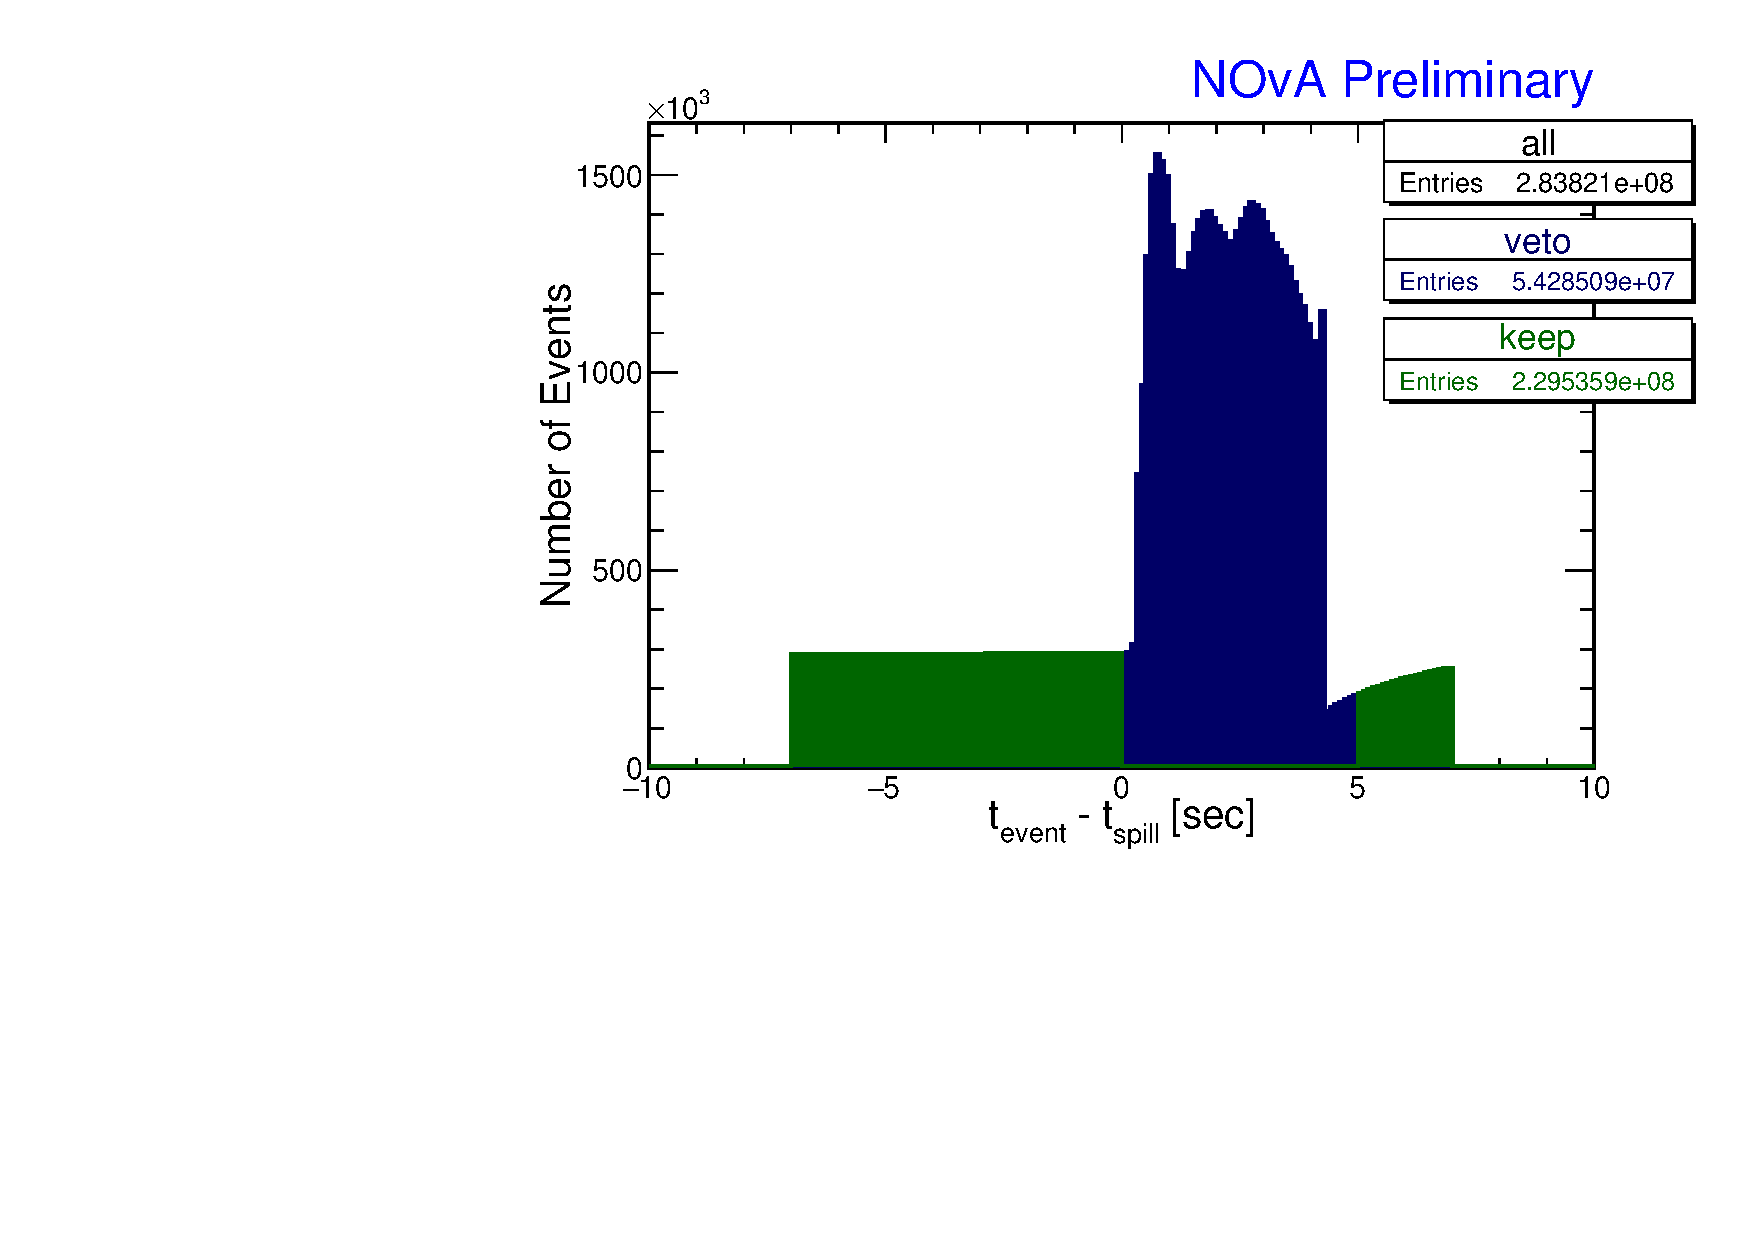
\includegraphics[width=\textwidth]{Plots/TBCalibration/RemoveTBSpills.pdf}
\caption[Removing Test Beam beam spill]{Test Beam beam spill events removed (blue) from the calibration samples. The remaining events (green) should mostly consist of cosmic particles. This example and the numbers of entries are for the full period 4 Test Beam sample.}
\label{fig:RemoveTBSpills}
\end{figure}

\subsubsection*{Reconstruction}
To use data events in simulation, we need to reconstruct their vertex positions and their initial 4-momenta. We use the standard reconstruction methods from \gls{NOvA}, described in Sec.~\ref{sec:NOvAReconstruction}. First we take the raw hits and group them into slices. Then we reconstruct cosmic tracks using the window cosmic track algorithm (used for calibration samples). Since we also require the 4-momentum information we have to use the \gls{BPF} tracking algorithm to identify muons and assign their momenta. \gls{BPF} requires vertex and prong input information, which we get from a cosmic ray vertex and FuzzyK prong algorithms respectively. The first three steps are identical to the full reconstruction applied to both data and simulation to produce the calibration samples. Since we do not need a 4-momentum information for calibration, we do not need to use cosmic ray vertex, FuzzyK vertex, or the \gls{BPF} to create calibration samples.

\subsubsection*{Selection}\label{sec:DataBasedSimSelection}
After the reconstruction process, we proceed to select events based on their slice and \gls{BPF} track properties. The overview of all selection criteria and their corresponding cut values are listed in Tab.~\ref{tab:DataBasedSimEventSelection}. In detail, the following conditions are used to select cosmic muon events for the data-based simulation:
\begin{enumerate}
\item We only use successfully reconstructed 3D \gls{BPF} tracks with the muon assumption;
\item As we aim to select cosmic events originating outside the detector, we apply a cut based on the distance of each track's start position from the edges of the detector. This cut has a negligible impact on the \gls{BPF} tracks, as indicated by the minimal difference between the red and the dotted azure lines in Fig. \ref{fig:DataBasedSimCosZSelectionComparison};

\begin{figure}[!ht]
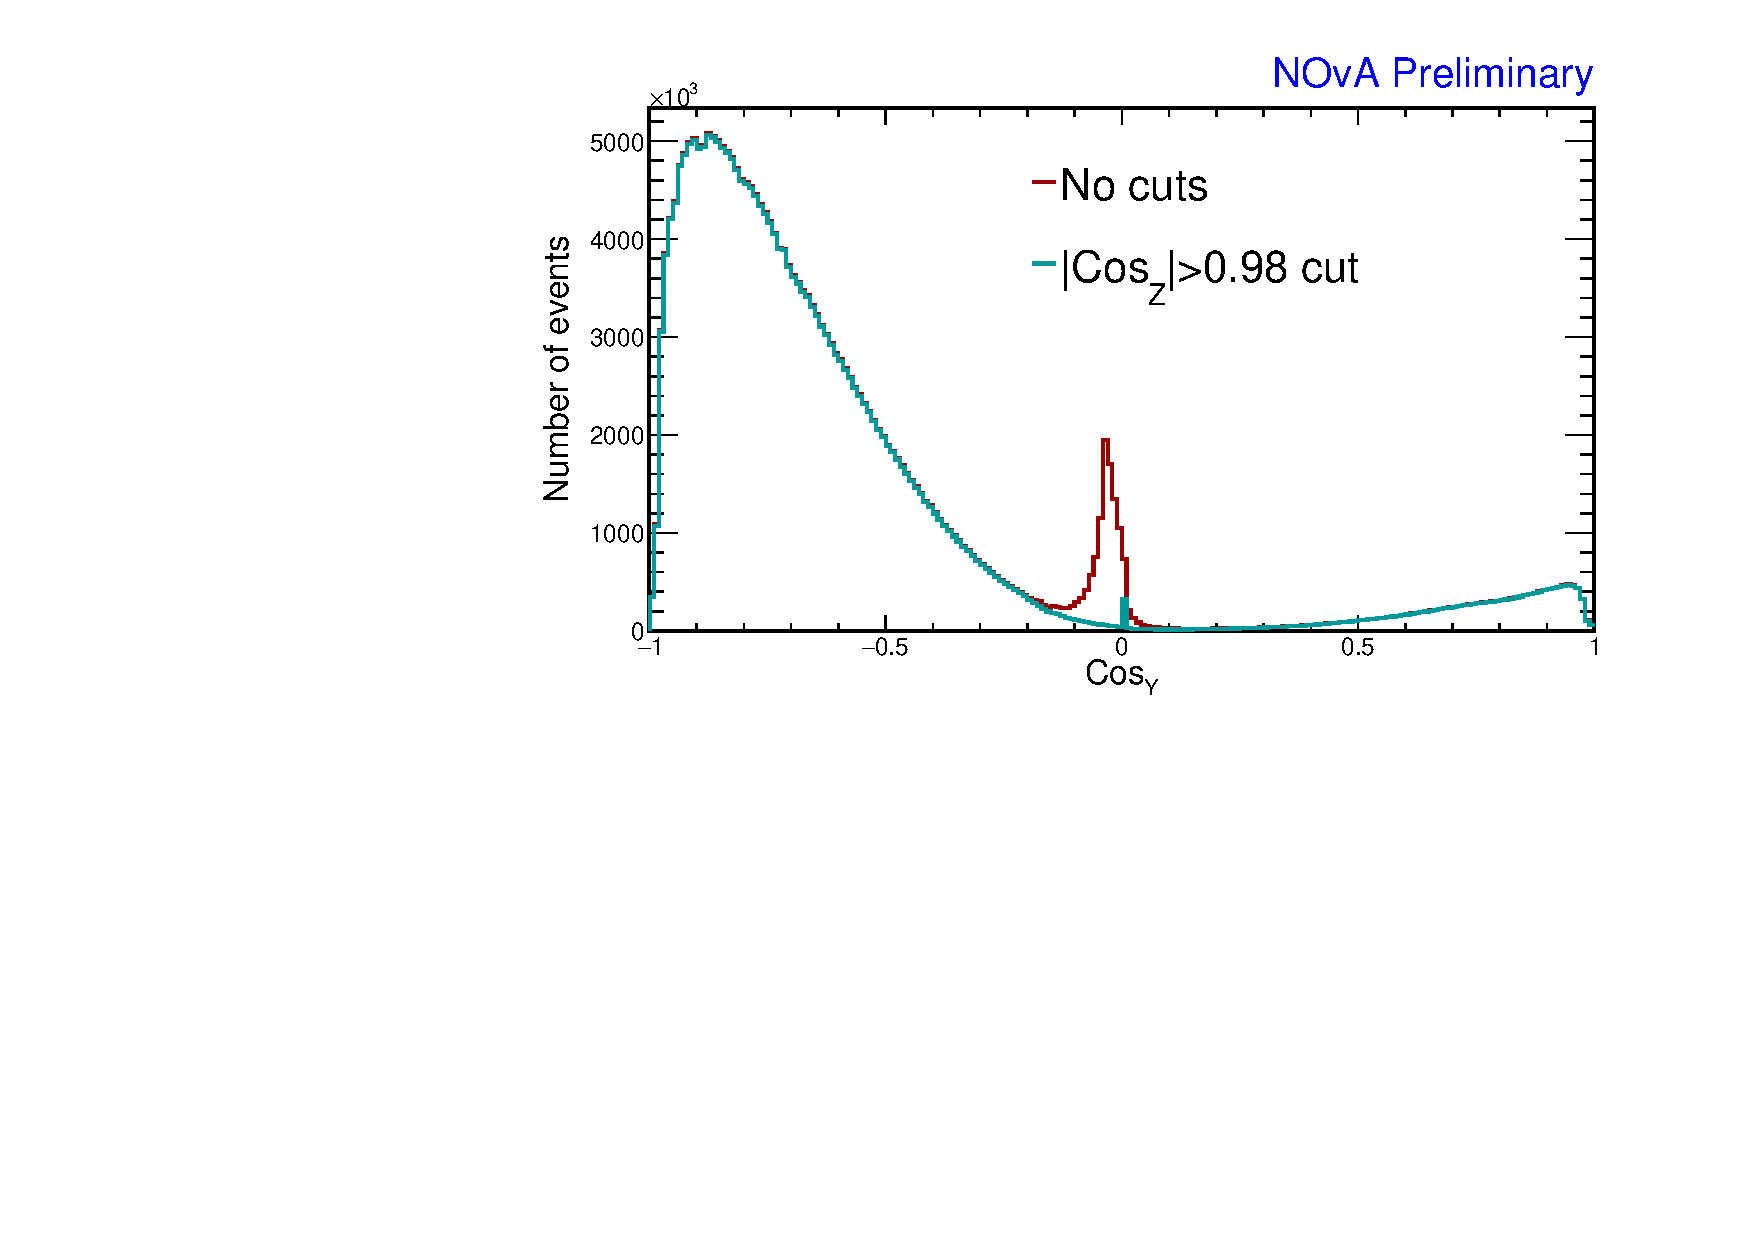
\includegraphics[width=\textwidth]{Plots/TBCalibration/DBSim_SelectionComparisonCosZCut_CosY.pdf}
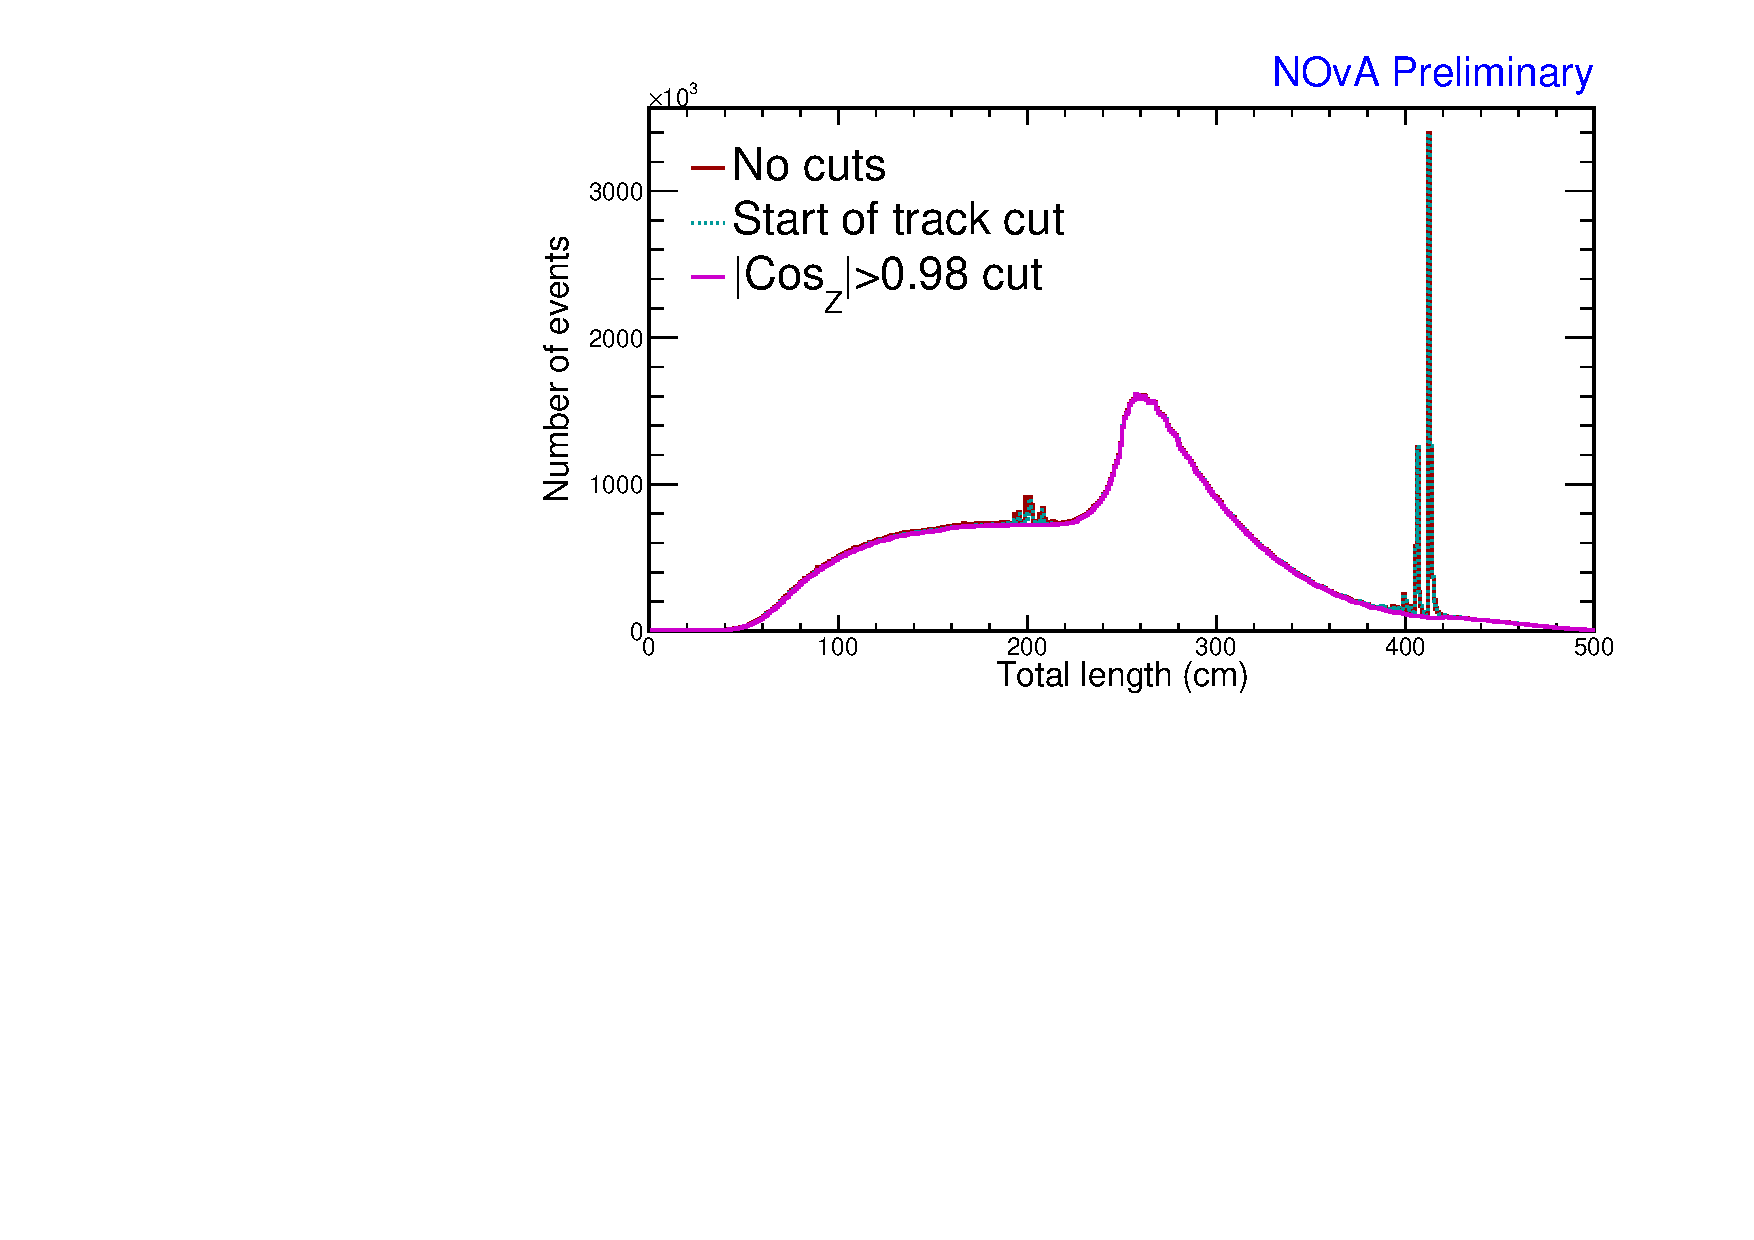
\includegraphics[width=\textwidth]{Plots/TBCalibration/DBSim_SelectionComparisonCosZCut_TotLength.pdf}
\caption[Track start and $\textsf{Cos}_Z$ cut for data-based simulation selection]{Impact of the cuts on the track start and on the maximum track angle from the z axis ($\textsf{Cos}_Z$) on the Test Beam data for the data-based simulation of cosmic muons. Top plot shows distribution of the angle from the y axis and bottom of the total track length, both made from the period 4 Test Beam data.}
\label{fig:DataBasedSimCosZSelectionComparison}
\end{figure}

\item We remove all events whose track is parallel to the beam direction, by requiring the angle from the z axis (parallel to the beam) to be $|\textsf{Cos}_Z|\leq 0.98$. Figure \ref{fig:DataBasedSimCosZSelectionComparison} demonstrates the presence of events peaked at track lengths of approximately $\unit[410]{cm}$ and $\unit[200]{cm}$, which correspond to the total and half length of the detector, respectively (or alternatively lengths of both blocks and of a single block). These events are strictly parallel to the beam direction and are likely remnants of beam events. Applying a cut on $\textsf{Cos}_Z$ effectively removes these events without affecting the rest of the data. This cut might only be needed for the Test Beam detector and not for the \gls{ND} and \gls{FD}, as it is likely these are particles scattered from the Test Beam beamline, or from the secondary beam. \note{Do we actually know why would there be a peak, even if small, after a single block? Is it due to reconstruction? Or more glue?}

\item To ensure that only events contributing to the final calibration sample are simulated, we use a selection based on the cuts used to select events for the data calibration samples (described in Sec.~\ref{sec:NOvACalibration} and listed as Calibration sample selection in Tab.~\ref{tab:DataBasedSimEventSelection}). We call these cuts the \textbf{calibration cuts}. However, there are two caveats we need to consider when applying the calibration cuts:
\begin{enumerate}
\item First, to create calibration samples, we apply the selection on tracks from the \textbf{window cosmic track} algorithm instead of the \gls{BPF} algorithm, which yield different distributions as depicted in Fig.~\ref{fig:DataBasedSimTrackComparison}. Notably, the \gls{BPF} tracks have a hard cut-off at the detector edges, whereas the window cosmic tracks are allowed to start beyond these limits. Also, as can be seen in the bottom plot of Fig.~\ref{fig:DataBasedSimBPFPeaks}, the \gls{BPF} tracks have a rugged distribution in $\textsf{Cos}_Z$, which is not present for window cosmic tracks. The origin of this shape is not exactly known, but it is likely caused by the detector structure, as shown in Fig.~\ref{fig:DataBasedSimBPFPeaks}. We concluded that the rugged shape should not have any impact on the resulting simulation. However given these differences between the tracking algorithms, applying the calibration cuts on the \gls{BPF} tracks could mistakenly remove events that would pass the same selection when applied to the window cosmic tracks.

\begin{figure}[!ht]
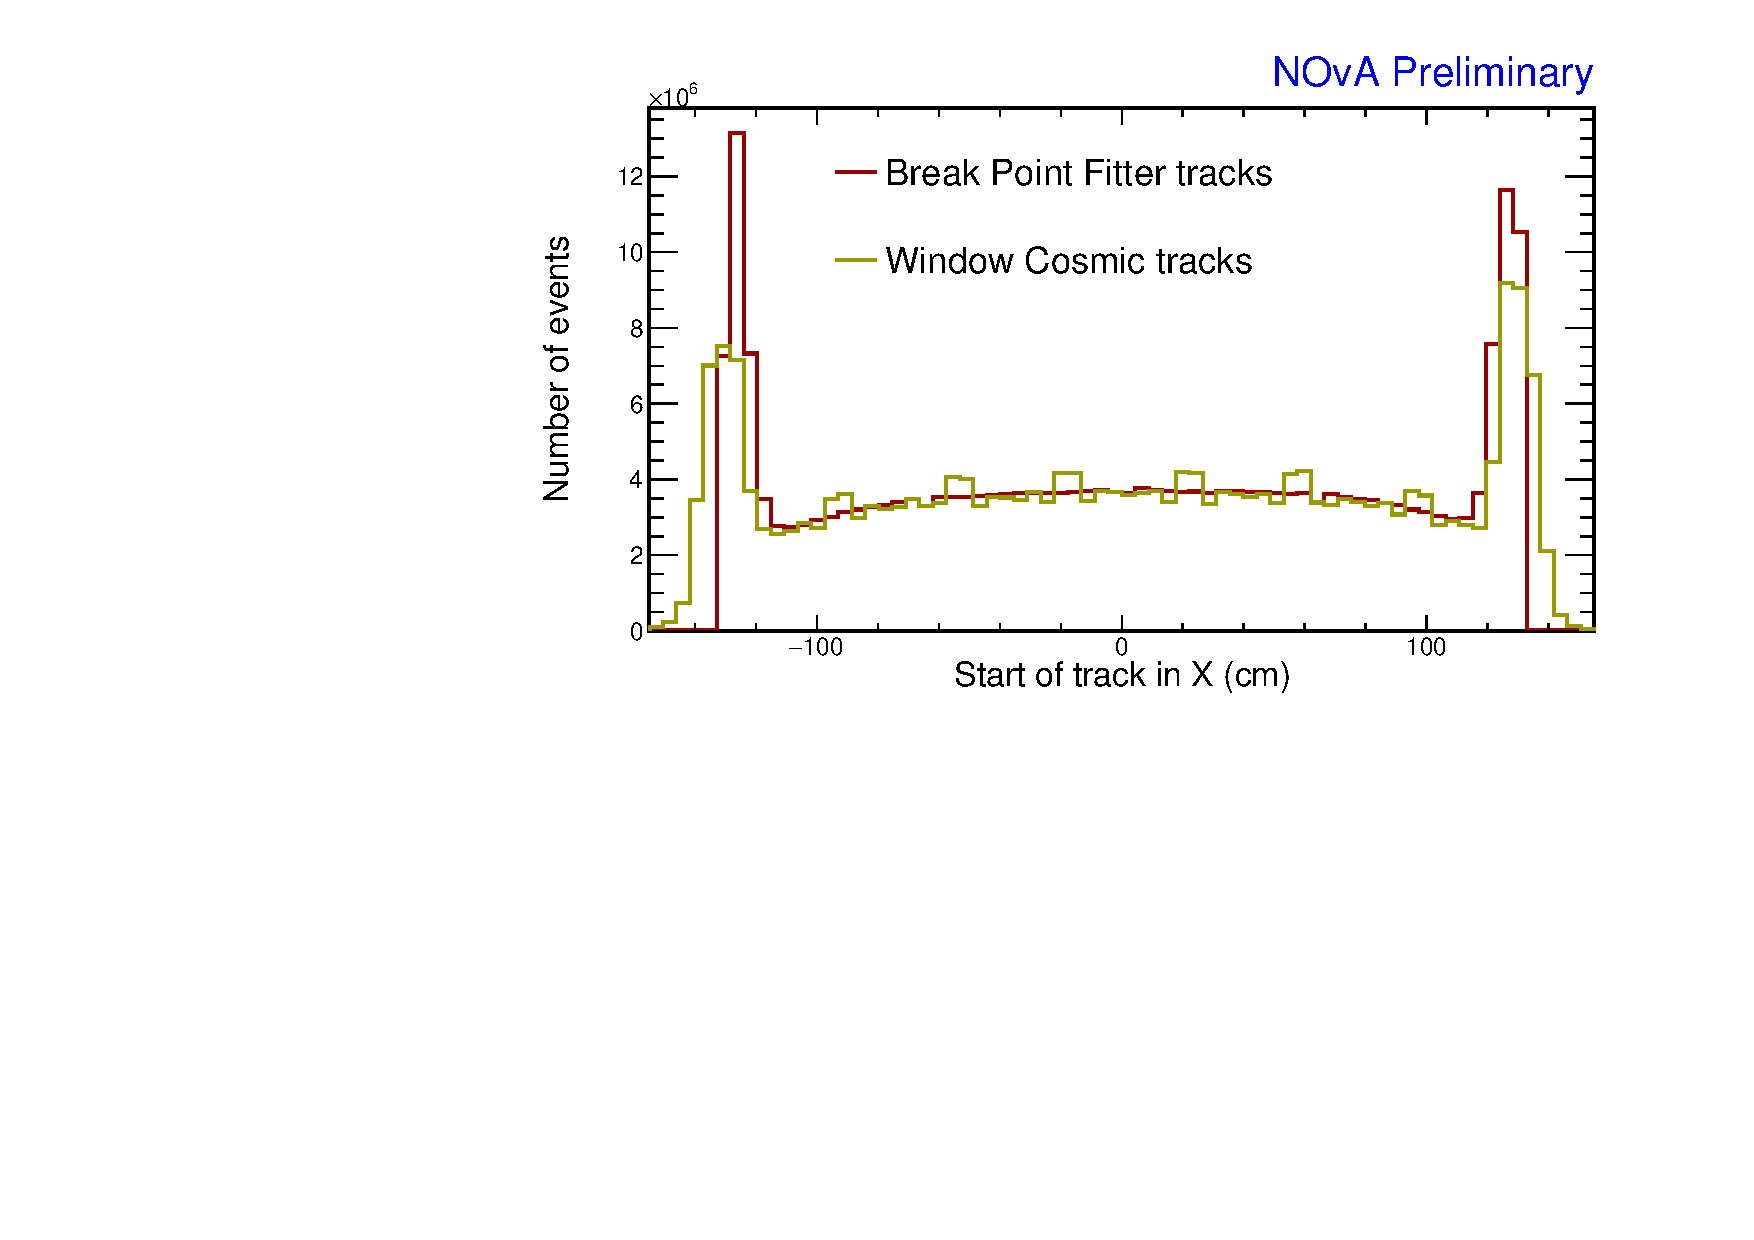
\includegraphics[width=\textwidth]{Plots/TBCalibration/DBSim_TrackAlgComparison_StartX.pdf}
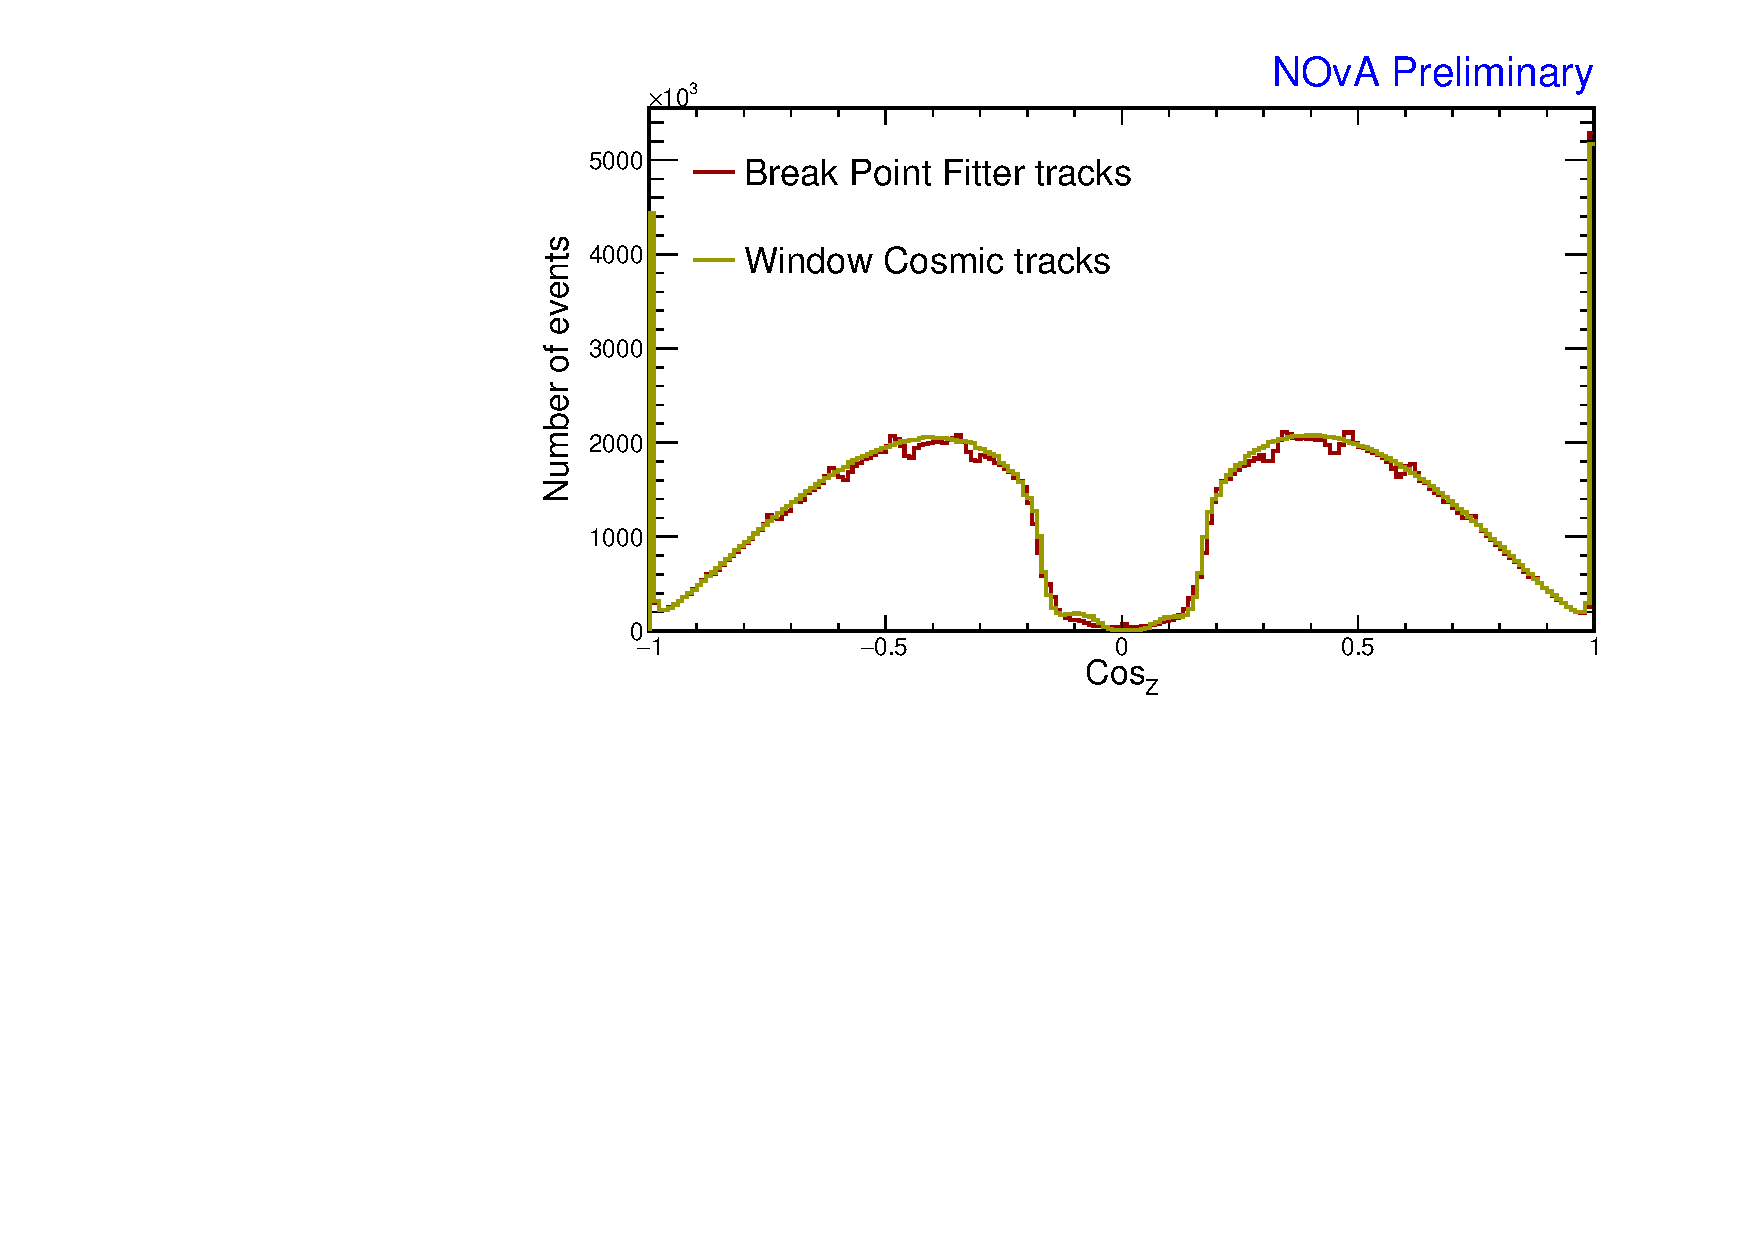
\includegraphics[width=\textwidth]{Plots/TBCalibration/DBSim_TrackAlgComparison_CosZ.pdf}
\caption[Tracking algorithms for the data-based simulation selection]{Difference between the tracks reconstructed with the \acrshort{BPF} and with the window cosmic track algorithms. Top plot shows the distribution of the start of track along the x axis and bottom plot shows the distribution of the angle from the z axis, both for the period 4 Test Beam data (with removed beam spill) without applying any selection.}
\label{fig:DataBasedSimTrackComparison}
\end{figure}

\begin{figure}[!hbtp]
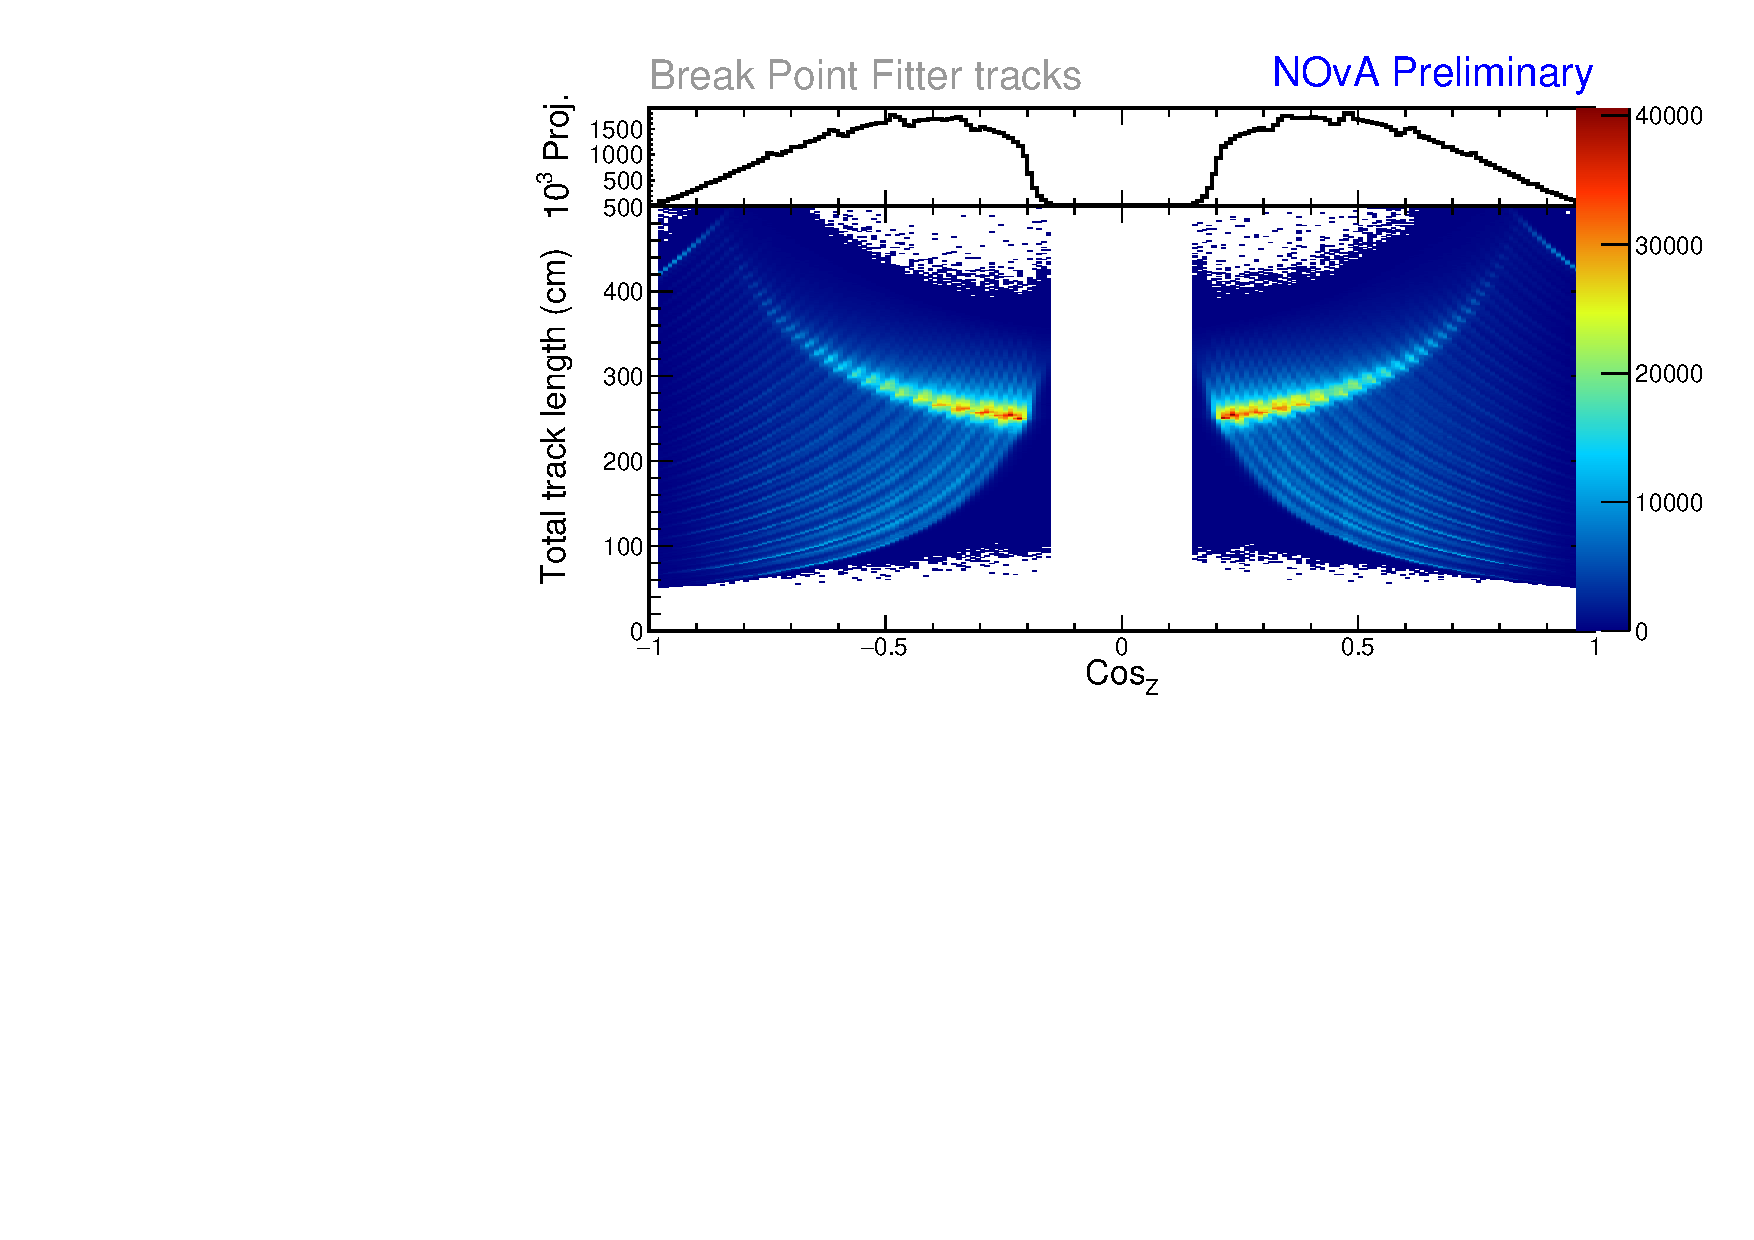
\includegraphics[width=\textwidth]{Plots/TBCalibration/DBSim_BPFPeaks_BPFTracks_dcosz_TotLength.pdf}
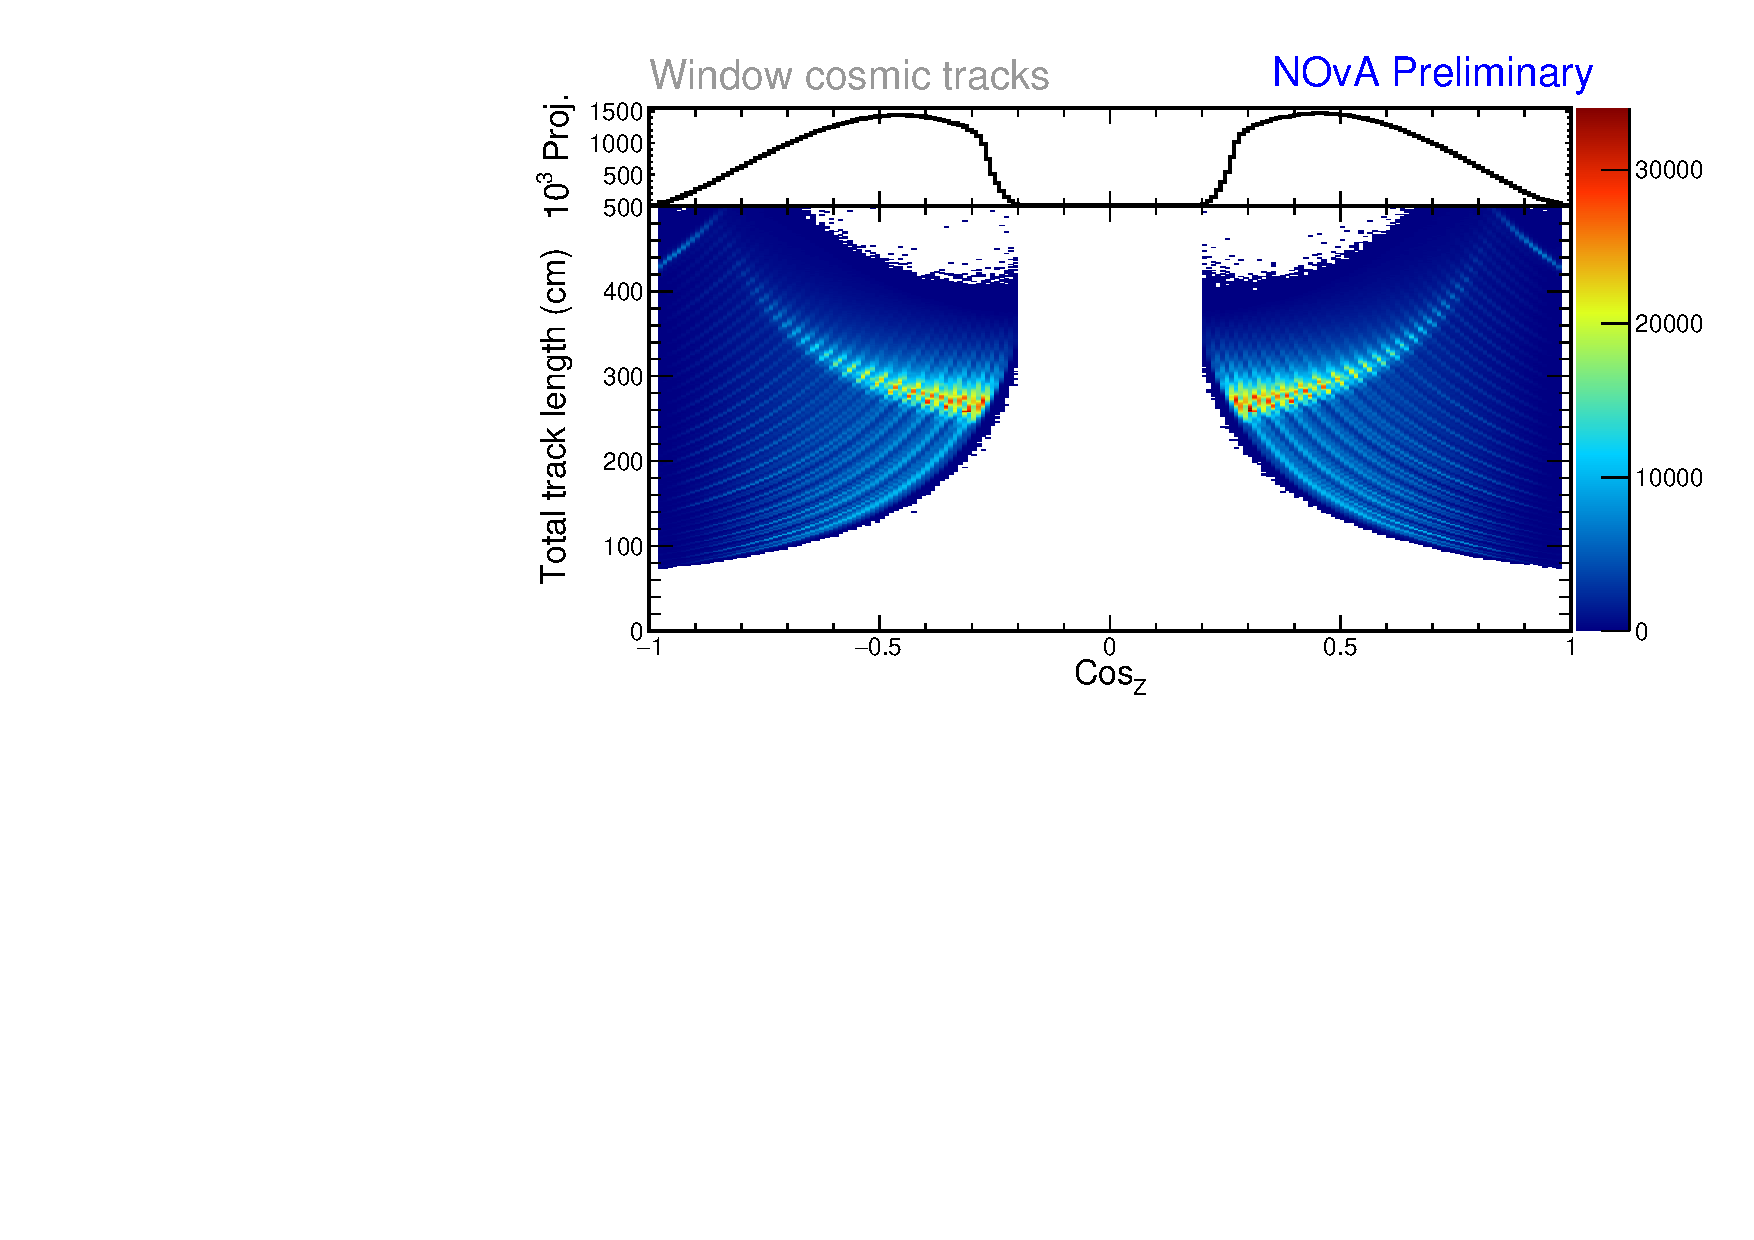
\includegraphics[width=\textwidth]{Plots/TBCalibration/DBSim_BPFPeaks_WTTracks_dcosz_TotLength.pdf}
\caption[Comparison of the $\textsf{Cos}_Z$ and track length distributions between tracking algorithms for the data-based simulation selection]{Comparison of the angle from the z axis ($\textsf{Cos}_Z$) and the total track length distributions between the \acrshort{BPF} tracks (top) and window cosmic tracks (bottom). Top parts of both plots show the 1D $\textsf{Cos}_Z$ distributions, scaled by $1/10^3$. The top plot is created with loose calibration cuts and the bottom plot with full calibration cuts per Tab.~\ref{tab:DataBasedSimEventSelection}, although this difference in selection shouldn't matter. These plots are investigating the origin of the rugged shape in the $\textsf{Cos}_Z$ distribution of \acrshort{BPF} tracks, as can be seen in the top part of the top plot. The long curved light blue/green lines in the 2D plots correspond to constant values of $\left|\textsf{Cos}_Z\right|\times\textsf{Tot. length} = \textsf{Tot. length}_Z$, equal to the extent of the track length in the z direction, and are distinct from each other due to the structure of the detector (segmentation into planes). It is clear that the \gls{BPF} tracks are peaked more sharply in $\textsf{Tot. length}_Z$ than the window cosmic tracks, which are more spread out. This discrepancy could cause the resulting shape in the $\textsf{Cos}_Z$ distribution of \acrshort{BPF} tracks. \note{To be honest I don't fully understand where do the BPF peaks come from, I but I have an idea and I'm hoping I'm explaining it enough here. If not, happy to discuss how to improve, cause I'm struggling to explain it well myself}}
\label{fig:DataBasedSimBPFPeaks}
\end{figure}

\item Second, each reconstruction algorithm has intrinsic deficiencies that can lead to misreconstructions. Therefore, applying the full calibration cuts on misreconstructed events may remove them, even though they would have passed if they were reconstructed correctly and hence they should have been included in the simulation. These events would then be missing from the resulting simulation sample, introducing a bias.\note{Is this clear enough as to what I mean? Also, is the tense use correct?}
\end{enumerate}

To address these concerns, we loosened the full calibration cuts to create a `buffer' around the selected events, allowing for fluctuations of the reconstruction algorithms while maintaining track quality. This way, events that would have been removed based on the calibration cuts applied to their reconstructed \gls{BPF} tracks, but kept based on the calibration cuts applied to their window cosmic tracks, now have a chance to make it into the final selection and therefore calibration sample. The differences between the full calibration cuts and the employed loosened calibration cuts applied to the \gls{BPF} tracks are listed in Tab.~\ref{tab:DataBasedSimEventSelection} and shown in Fig.~\ref{fig:DataBasedSimCalibCutsComparison}. There we also show the data calibration sample, which was created by applying the full calibration cuts on window cosmic tracks.
\end{enumerate}

\iffalse
The cuts are:
\begin{itemize}
\item Tracks must have at least two X and two Y cells
\item The difference between the start and stop Z position of the track must be at least 70~cm
\item The Z component of the initial direction vector of the track must be at least 0.2
\item At least 80\% of cells in slice must be reconstructed into the track in both X and Y views
\item At most 6 cells were hit per plane
\item Maximum difference between the first planes in X and Y is 3 (same for the last planes)
\item The difference between number of planes crossed in X and Y view must be at most 10\% of the total number of planes crossed
\item Remove tracks where a step between trajectory points is more than this value * the median step size
\end{itemize}
\fi

\begin{table}[!ht]
\centering
\caption[Overview of the event selection for the data-based simulation]{Event selection of cosmic muons used for the data-based simulation (in green under Loose selection) and comparison to the Full selection cuts used to create the calibration samples (described in Sec.~\ref{sec:NOvACalibration}) in blue. The last two rows are not used for Test Beam, but are employed for the \acrshort{ND} and \acrshort{FD}.}
\begin{tabular}{clcc}
& \multirow{2}{*}{\centering{\textbf{Cut}}} & \multicolumn{2}{c}{\textbf{Selection}}\\
& & \cellcolor[HTML]{3166FF}\textbf{Full} & \cellcolor[HTML]{32CB00}\textbf{Loose}\\\hline
                                   & Muon assumption and 3D track from BPF         &                                             &                                          \\
                                   & Max. track start distance from edge                       & \multicolumn{2}{c}{50 cm}                                                                 \\
                                   & Max. $Cos_{Z}$                                            & \multicolumn{2}{c}{0.98}                                                               \\ \hline
                                   & Min. number of hits in X or Y                             & \multicolumn{2}{c}{\cellcolor[HTML]{FFFFFF}2}                                          \\
                                   & Min. difference between Stop$_{Z}$ and Start$_{Z}$        & \cellcolor[HTML]{3166FF}70~cm                 & \cellcolor[HTML]{32CB00}50~cm             \\
                                   & Min. $Cos_{Z}$ & \cellcolor[HTML]{3166FF}0.2                 & \cellcolor[HTML]{32CB00}0.15             \\
                                   & Min. frac. of slice hits in track in each view    & \multicolumn{2}{c}{0.8}                                                                \\
                                   & Max. number of cells per plane in each view               & \cellcolor[HTML]{3166FF}6                   & \cellcolor[HTML]{32CB00}15               \\
                                   & Max. difference in X-Y for first (last) plane     & \cellcolor[HTML]{3166FF}3                   & \cellcolor[HTML]{32CB00}5                \\
                                   & Max. plane asymmetry                                      & \cellcolor[HTML]{3166FF}0.1                 & \cellcolor[HTML]{32CB00}0.2              \\
                                   & Max. step size to median step size ratio                  & \cellcolor[HTML]{3166FF}3                   & \cellcolor[HTML]{32CB00}5                \\
                                   & \cellcolor[HTML]{C0C0C0}Max. vertex distance from edge    & \multicolumn{2}{c}{\cellcolor[HTML]{C0C0C0}10~cm}                                         \\
\parbox[t]{2mm}{\multirow{-10}{*}{\rotatebox[origin=c]{90}{Calibration sample selection}}}& \cellcolor[HTML]{C0C0C0}Max. track end distance from edge & \multicolumn{2}{c}{\cellcolor[HTML]{C0C0C0}10 cm}
\end{tabular}
\label{tab:DataBasedSimEventSelection}
\end{table}

\begin{figure}[!h]
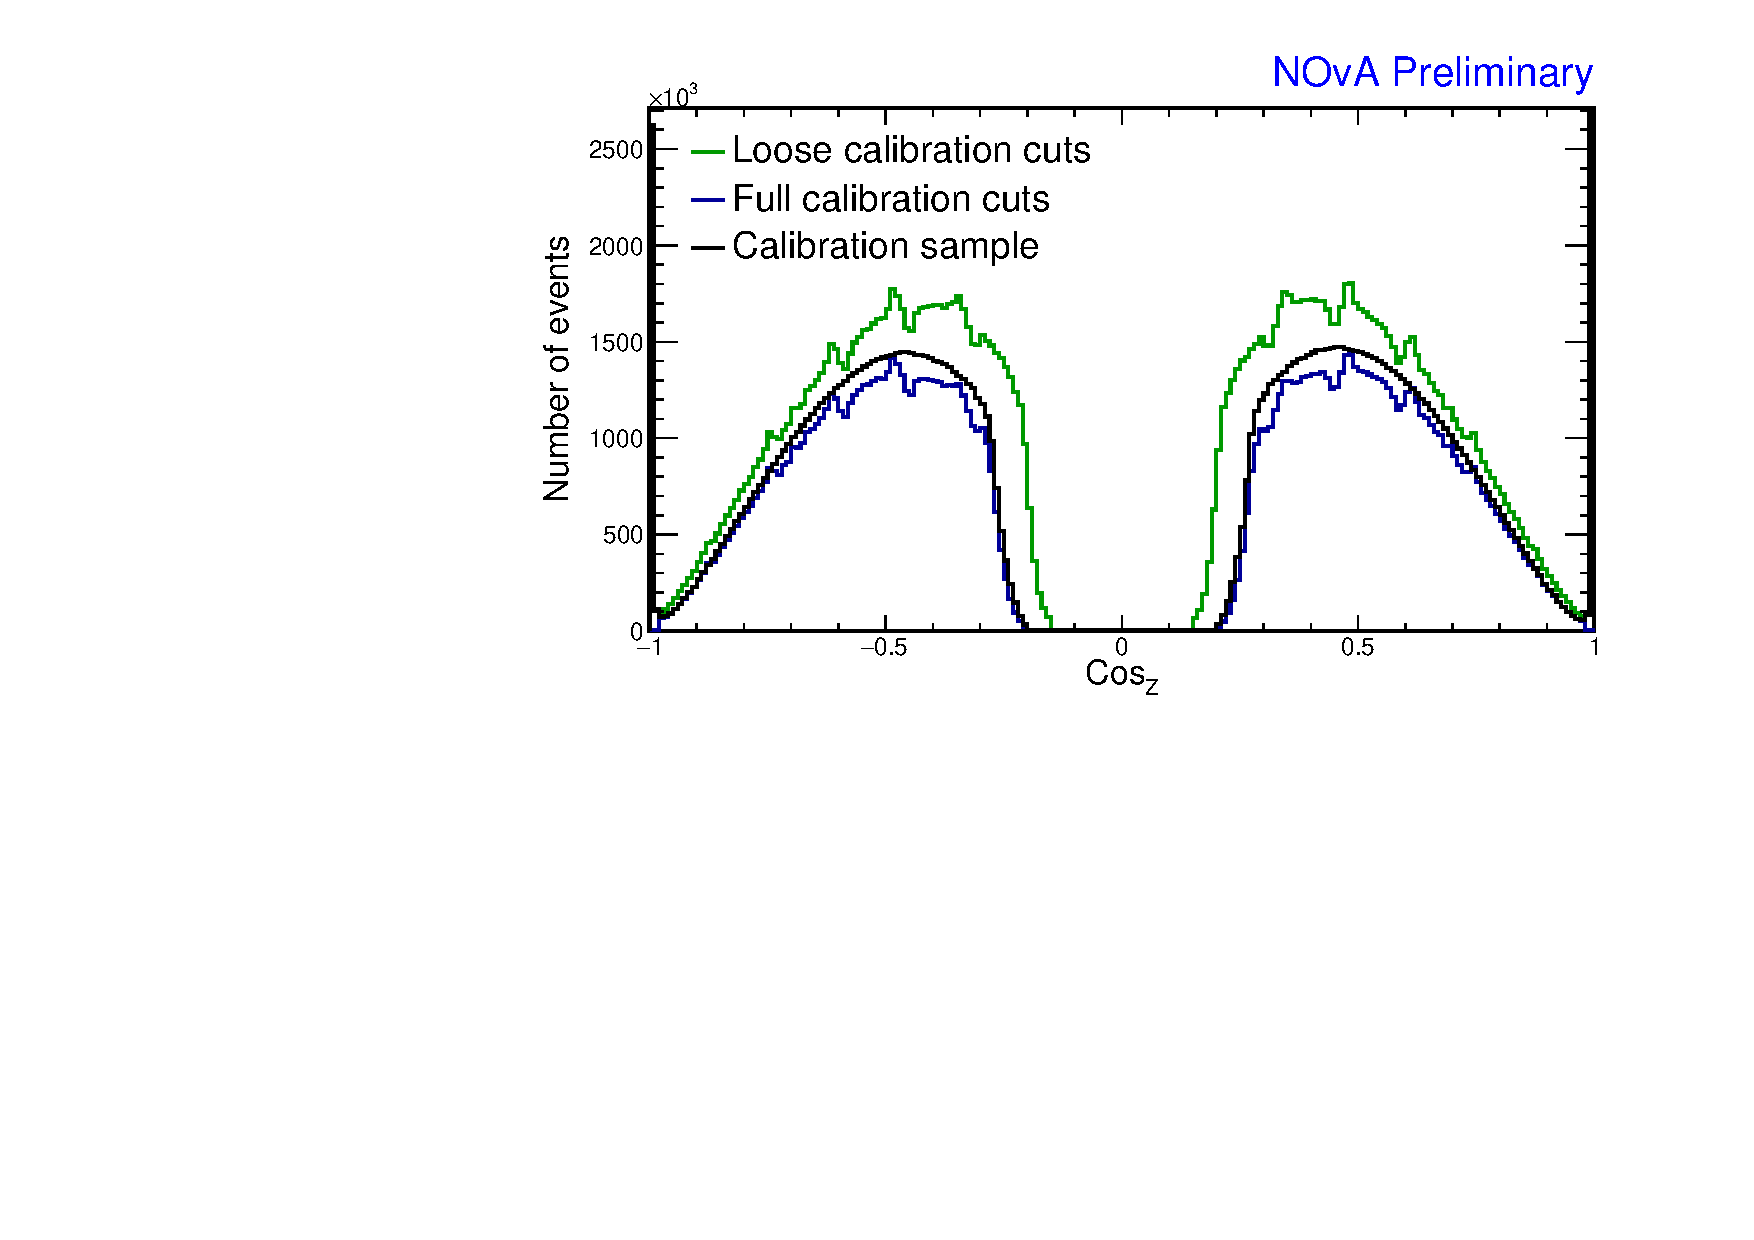
\includegraphics[clip, width=\textwidth]{Plots/TBCalibration/DBSim_SelectionComparisonPCHitsListCut_CosZ.pdf}
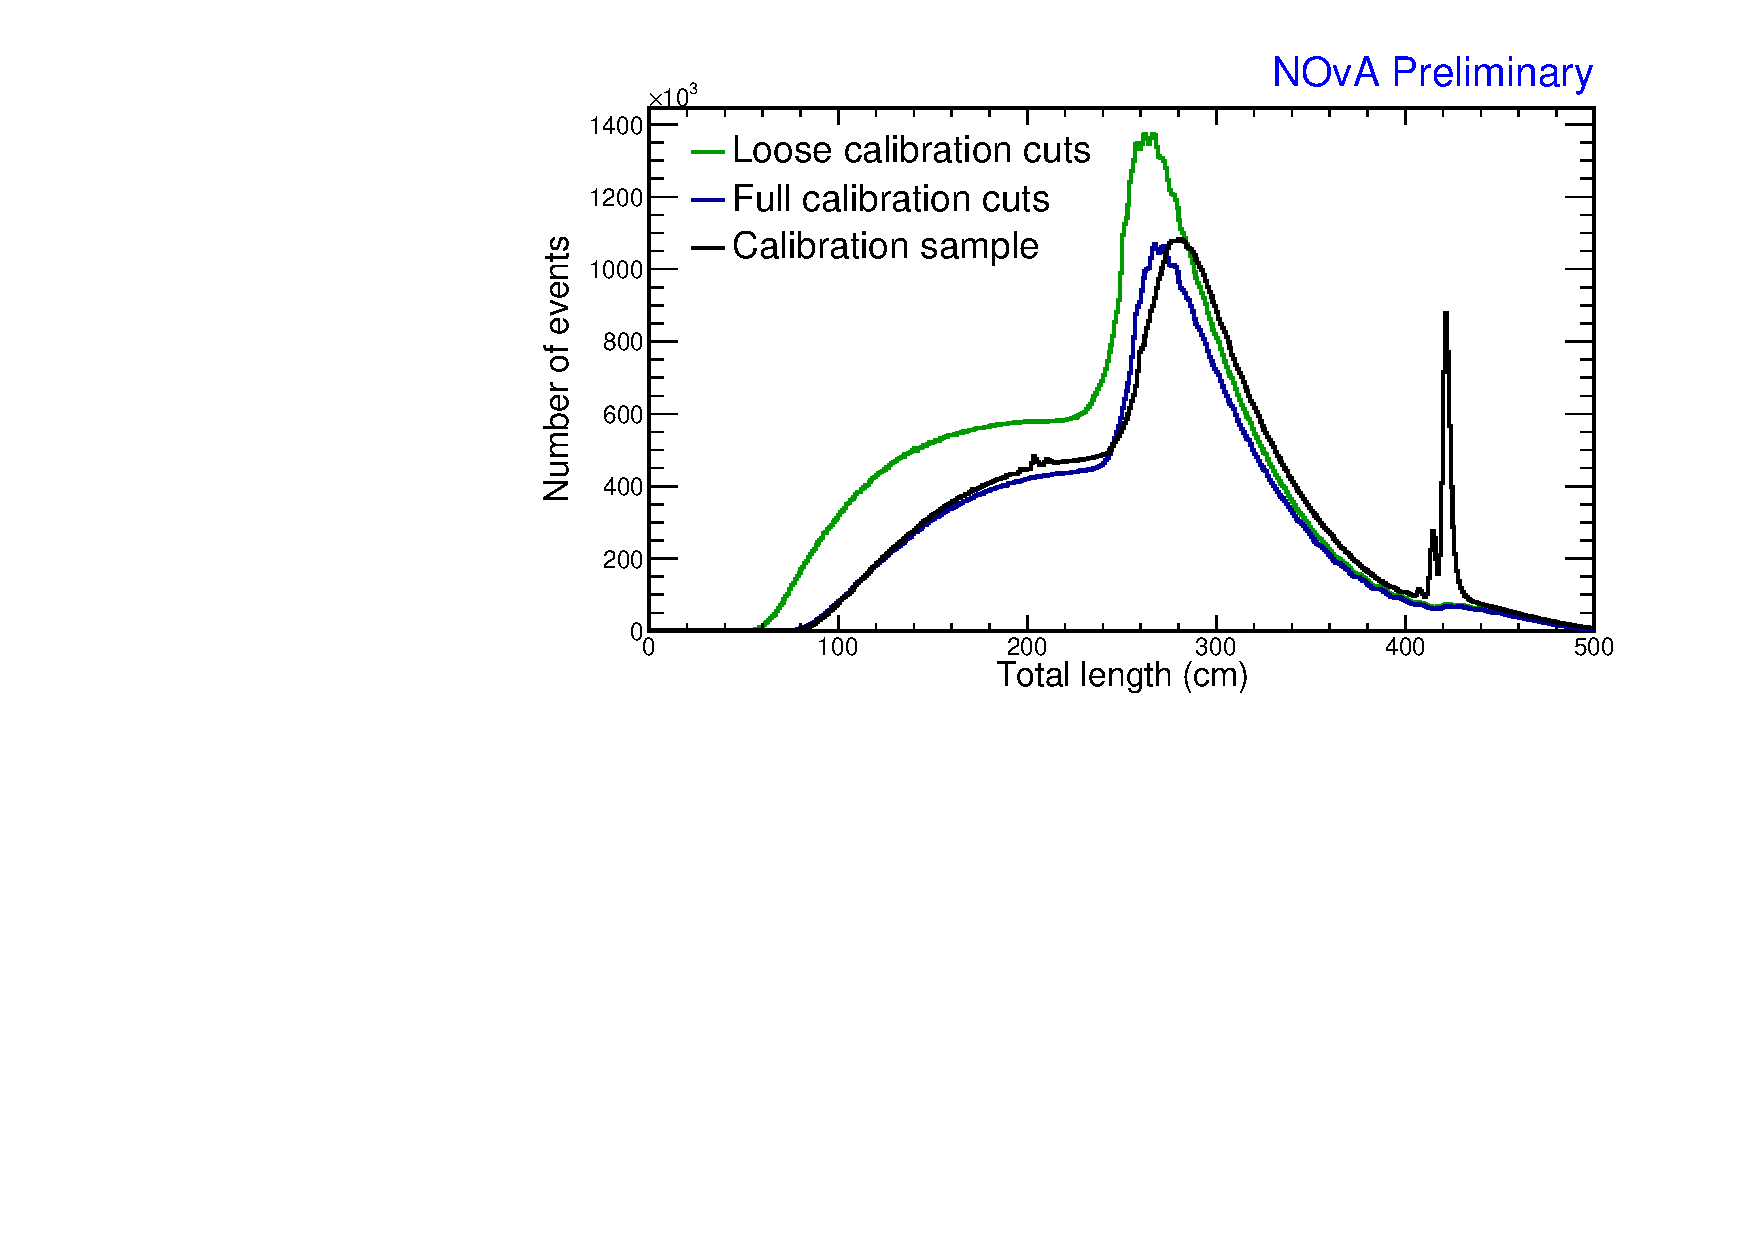
\includegraphics[clip, width=\textwidth]{Plots/TBCalibration/DBSim_SelectionComparisonPCHitsListCut_TotLength.pdf}
\caption[Event selection for the data-based simulation]{Comparison of full and loose event selections for the data-based simulation as per Tab.~\ref{tab:DataBasedSimEventSelection} and of the corresponding data calibration sample in black. As described in text, the loose calibration cuts applied to the \acrshort{BPF} tracks (green) were used for simulation to mitigate the discrepancy between applying the full calibration cuts to the \acrshort{BPF} tracks (blue) and the window cosmic tracks (black). All of the distributions are made from the period 4 Test Beam data.}
\label{fig:DataBasedSimCalibCutsComparison}
\end{figure}

During the selection process, we determine whether the muon is stopping inside the detector or passing through, based on the end position of the reconstructed track. For Test Beam we say it is a stopping muon if its track ends at least $\unit[20]{cm}$ from any edge of the detector. For the \gls{ND} and \gls{FD} this is $\unit[50]{cm}$. This information assists in correcting the energy of through-going muons, as outlined in the following Sec.~\ref{sec:DataBasedSimPython}.

%\FloatBarrier
\subsection{Energy Correction, Charge Assignment and Smearing}\label{sec:DataBasedSimPython}
Once we have the kinematic information for the selected events, we perform several tasks to get the final sample of cosmic muons for the data-based simulation. This includes correcting energies of the through-going muons, assigning a charge to each muon event, and smearing and converting the information into the correct format required by the generator.

\subsubsection*{Energy Correction}
Through-going muons do not deposit all of their energy inside the detector. Therefore we cannot reliably calculate their initial energies from the reconstructed information, but we can estimate an energy that could leave the same track. In general, the energy spectrum of cosmic muons can be approximately described by a power law $E^{-\alpha}$, with $\alpha\approx2.7$ \cite{NOvA-doc-51327,rpp2022-rev-cosmic-rays.pdf}. The expectation value for the `true' initial energy of through-going muons can be therefore calculated as
\begin{equation}
\left\langle E\right\rangle =\frac{\int^{E_C}_{E_R} E\cdot E^{-\alpha}}{\int^{E_C}_{E_R} E^{-\alpha}}=\left(\frac{\alpha -1}{\alpha -2}\right)\left(\frac{E_C^{2-\alpha}-E_R^{2-\alpha}}{E_C^{1-\alpha}-E_R^{1-\alpha}}\right),
\end{equation}
where $E_R$ is the reconstructed energy we got from the \gls{BPF}. $E_C$ is the critical energy chosen conservatively to be $\unit[300]{GeV}$, as we do not expect muons with higher energies to be selected due to large showers along their paths. We use this corrected initial energy for all muons that do not stop inside the detector, as identified during selection described in Sec.~\ref{sec:DataBasedSimSelection}. Figure \ref{fig:DataBasedSimEnergyScaling} shows the corrected energy distribution of our selected events and demonstrates that the choice of the critical energy does not significantly change the correction. 

\begin{figure}[hbtp]
\centering
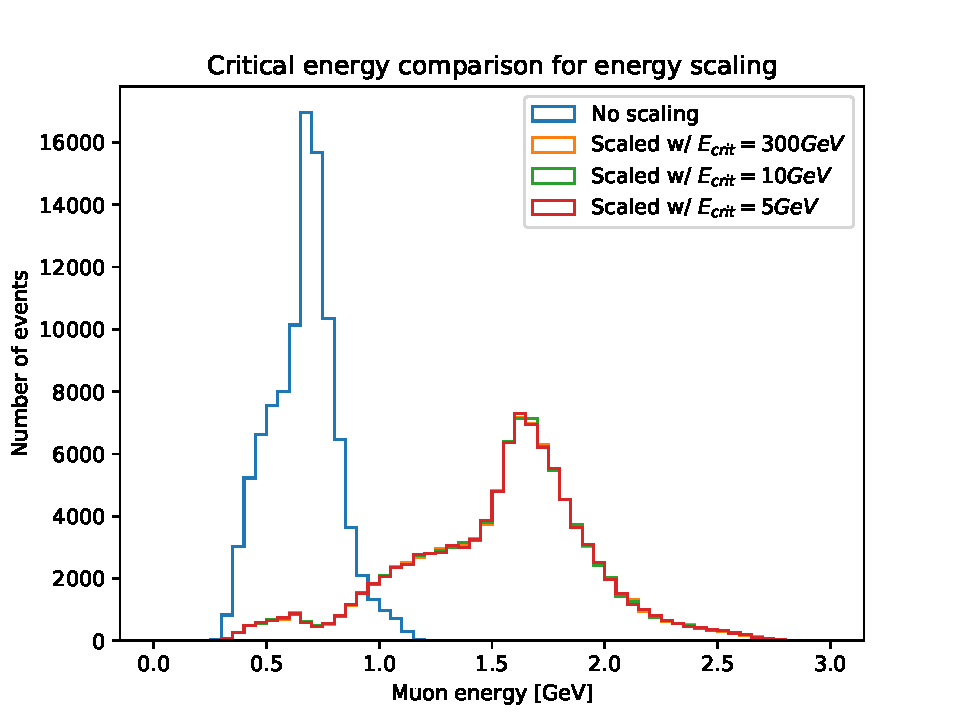
\includegraphics[width=0.8\textwidth]{Plots/TBCalibration/DBSim_ECritComparison.pdf}
\caption[Energy correction for through-going muons for the data-based simulation]{The effect of energy correction for through-going muons with various critical energies. No significant difference can be seen when using different critical energies.}
\label{fig:DataBasedSimEnergyScaling}
\end{figure}

This corrected energy is however \textbf{not} a good representation of the true energy spectrum of cosmic muons at surface level and getting a correct energy distribution from data would require a much more dedicated effort. The corrected energy would also be different for different \gls{NOvA} detectors, since the reconstructed energy is calculated from the track length. For example, the corrected energy of cosmic muons when entering the detector would be larger for the bigger \gls{ND} than for Test Beam, even though the \gls{ND} is underground. 

However, since this simulation is intended to be used for calibration, where we use through-going muons only for relative calibration, we do not need a perfect representation of the cosmic muon energy spectrum. Not including more energetic cosmic muons into the simulation does bias the energy deposition towards lower values, but this is corrected for during absolute calibration which only uses stopping muons, for which we assume we reconstruct their energy well from \gls{BPF}.

If someone were to use this simulation for something other than calibration, it would be necessary to rethink the energy correction, either by changing the energy estimation from track based algorithms to energy deposition, or by including information from external sources. It would also be necessary to include angular dependence for the energy correction as described in the PDG \cite{rpp2022-rev-cosmic-rays.pdf}.

\subsubsection*{Smearing}
The reconstructed distributions in data are influenced by the detector structure, reconstruction efficiencies and other effects that can bias the simulation. To avoid this influence, we smear the reconstructed values by randomly varying
\begin{itemize}
\item the total momentum within 2\%,
\item the azimuthal angle uniformly,
\item the polar angle within $\unit[4]{mrad}$,
\item and the x, y and z vertex positions within the width or depth of the cell respectively.
\end{itemize}

\subsubsection*{Charge Assignment}
We need to tell the detector simulation whether to simulate a muon or an anti-muon. However we do not reconstruct the charge of the muons, so we have to randomly assign it based on a statistical distribution from external measurements. The probability that a muon has a positive charge can be expressed as \cite{NOvA-doc-51327} 

%Figure out where are the plots and the equation Mark/Teresa quoted from (somewhere in PDG). Describe the basis of the measurement.
%Here(p10): https://pdg.lbl.gov/2022/reviews/rpp2022-rev-cosmic-rays.pdf
%But the equation must be from one of the sources listed.

\begin{equation}
P_+ \simeq 0.539 + \frac{x}{34.5}-\left(\frac{x}{9.48}\right)^2 + \left(\frac{x}{8.27}\right)^3,
\end{equation}
where $x$ is the logarithm of the total momentum in $\unit{GeV}$.

\subsubsection*{Running the Simulation}
We save the vertex positions, the four momenta and the assigned charge into a text file, that is then fed into the same detector and readout simulation chain, as was described for the \gls{ND} and \gls{FD} in Sec.~\ref{sec:NOvASimulation}.  We use the fibre brightness map that is used in calibration (see Sec.~\ref{sec:NOvACalibration}) to inform the simulation about the real detector conditions. Since we want the simulated detectors to be functional copies of the ideal versions of the real detectors, it is important to provide a correct brightness file without any defects. For this simulation we use the fibre brightness map described in Sec.~\ref{sec:FibreBrightnessTB}.

\subsection{Validation}
To validate whether the newly created simulation works as expected, we create the simulation calibration sample using the reconstruction and selection of cosmic muons for calibrations described in Sec.~\ref{sec:NOvACalibration}. We then compare this to the equivalent data calibration sample, created from the same data that was used to seed the simulation. Additionally, we use the newly simulated events as `fake data' and pass them through the same reconstruction, selection and simulation processes as were used to create the first iteration, hence creating a `re-simulation' sample. This is used to validate the stability of the simulation process.

The data-simulation comparisons are shown in Fig.~\ref{fig:DataBasedSimDataMCComparison_cosXcosY}-\ref{fig:DataBasedSimDataMCComparison_startZ}. The data and simulation calibration samples are shown in black and pink solid lines respectively. Both are equivalent to applying the full calibration cuts to the window cosmic tracks, as described in Sec.~\ref{sec:DataBasedSimSelection}. For comparison, we are also showing distributions of the \gls{BPF} tracks with full and loose calibration cuts in blue and green dashed lines respectively. We are expecting that the distributions of the simulation calibration sample (pink) match the distributions of the data calibration sample (black), without being affected by the different shape of the \gls{BPF} tracks (dashed lines).

\begin{figure}[!ht]
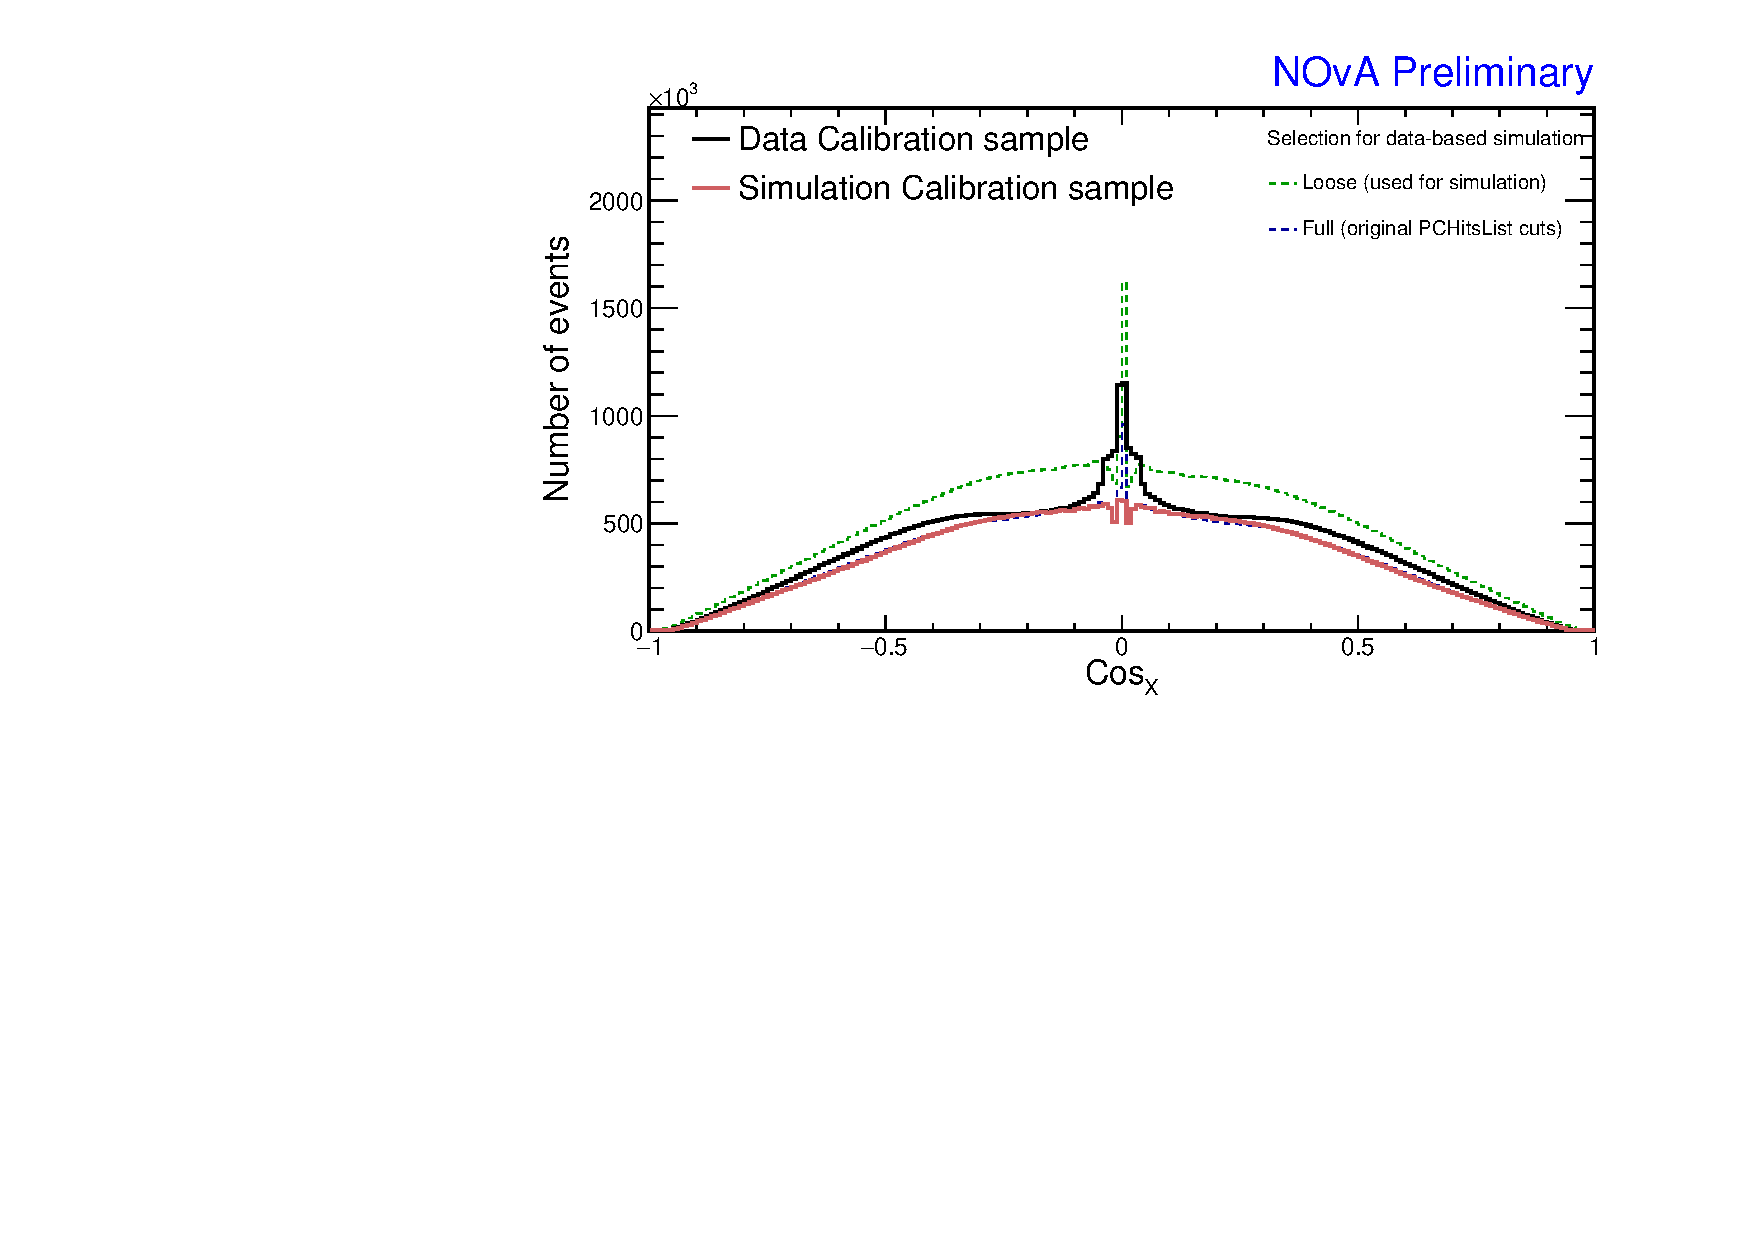
\includegraphics[width=\textwidth]{Plots/TBCalibration/DBSim_DataMCComparison_CosX.pdf}
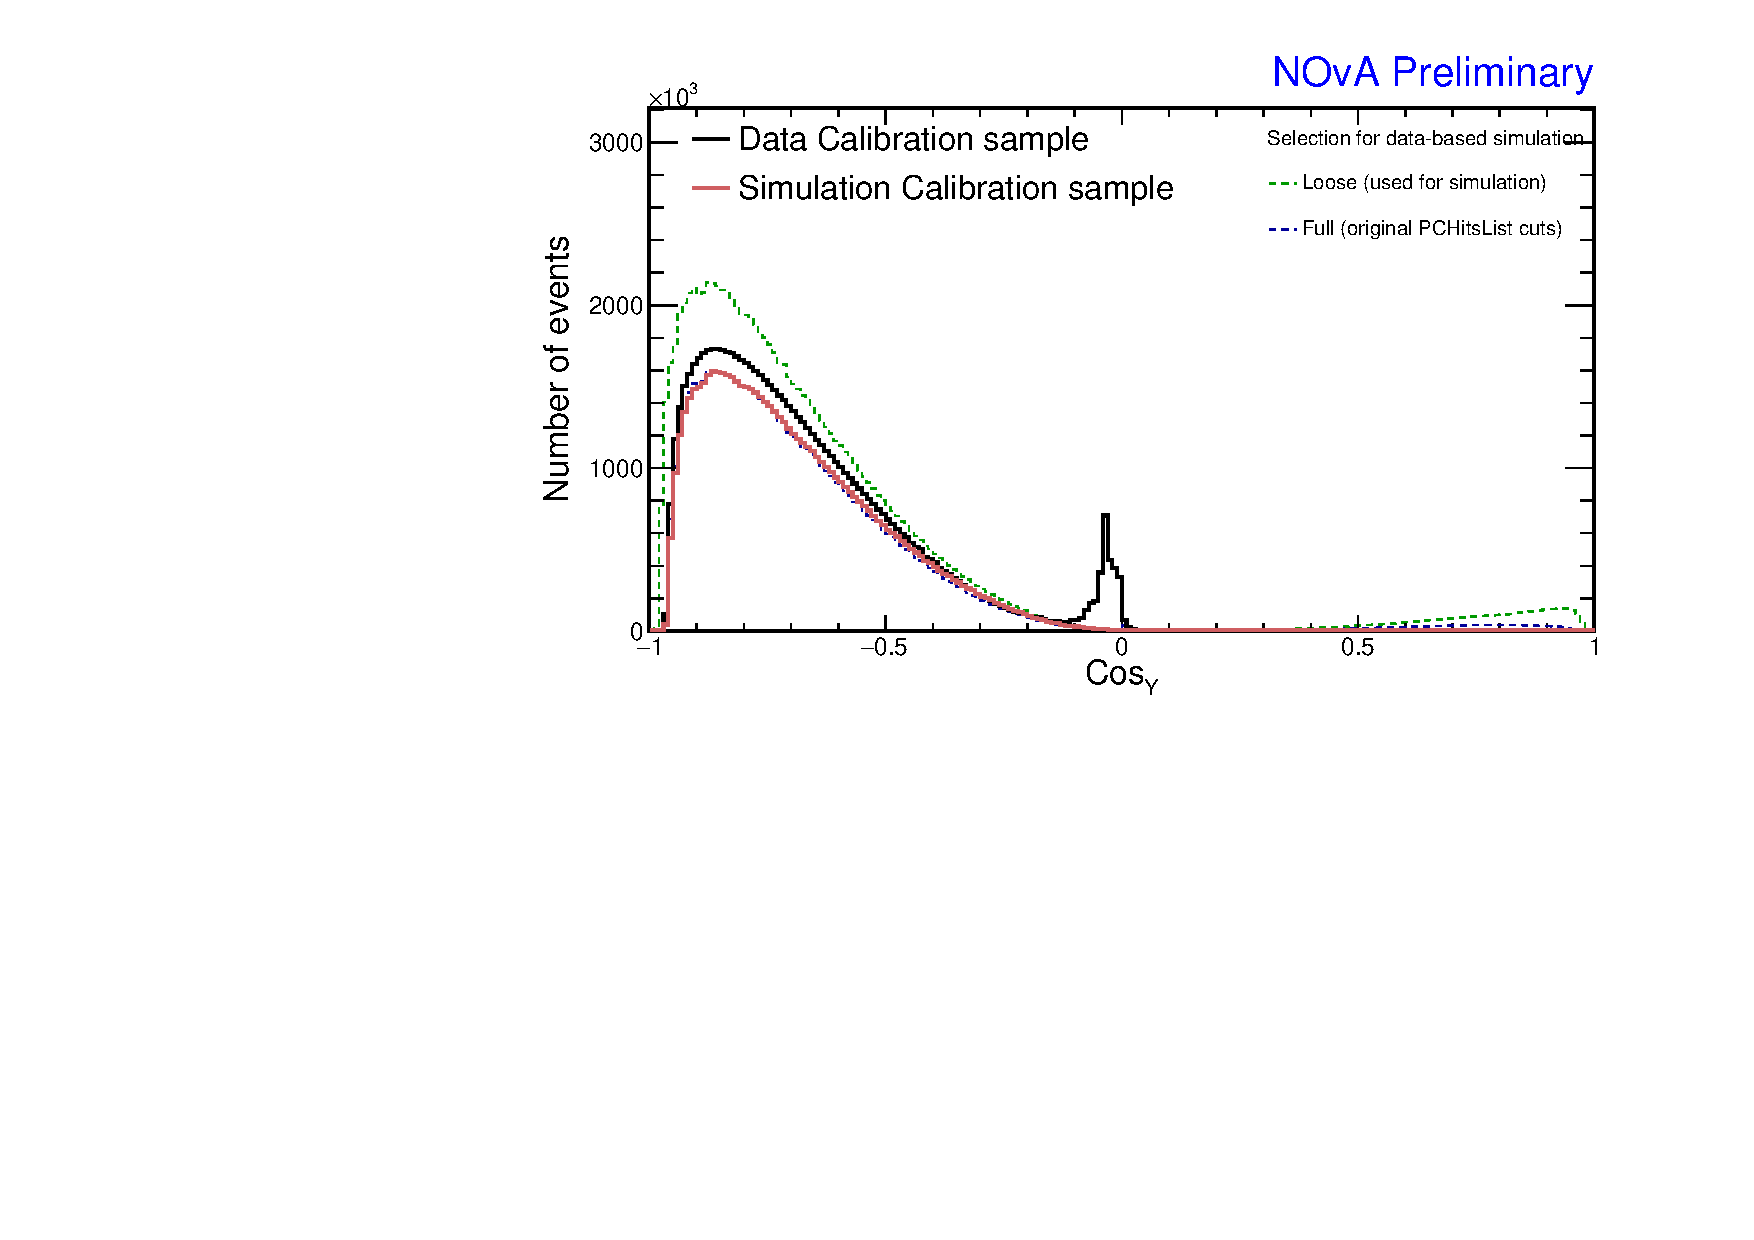
\includegraphics[width=\textwidth]{Plots/TBCalibration/DBSim_DataMCComparison_CosY.pdf}
\caption[Data-Simulation comparison of angular distributions]{Comparison of the angle from the x axis (top) and y axis (bottom) between the data (black) and simulation (pink) calibration samples, as detailed in the text. Additionally, the distributions of data with full (blue) and loose (green) selections applied to the \acrshort{BPF} tracks are shown, where the loose selection was used to create the simulation.}
\label{fig:DataBasedSimDataMCComparison_cosXcosY}
\end{figure}

\begin{figure}[!ht]
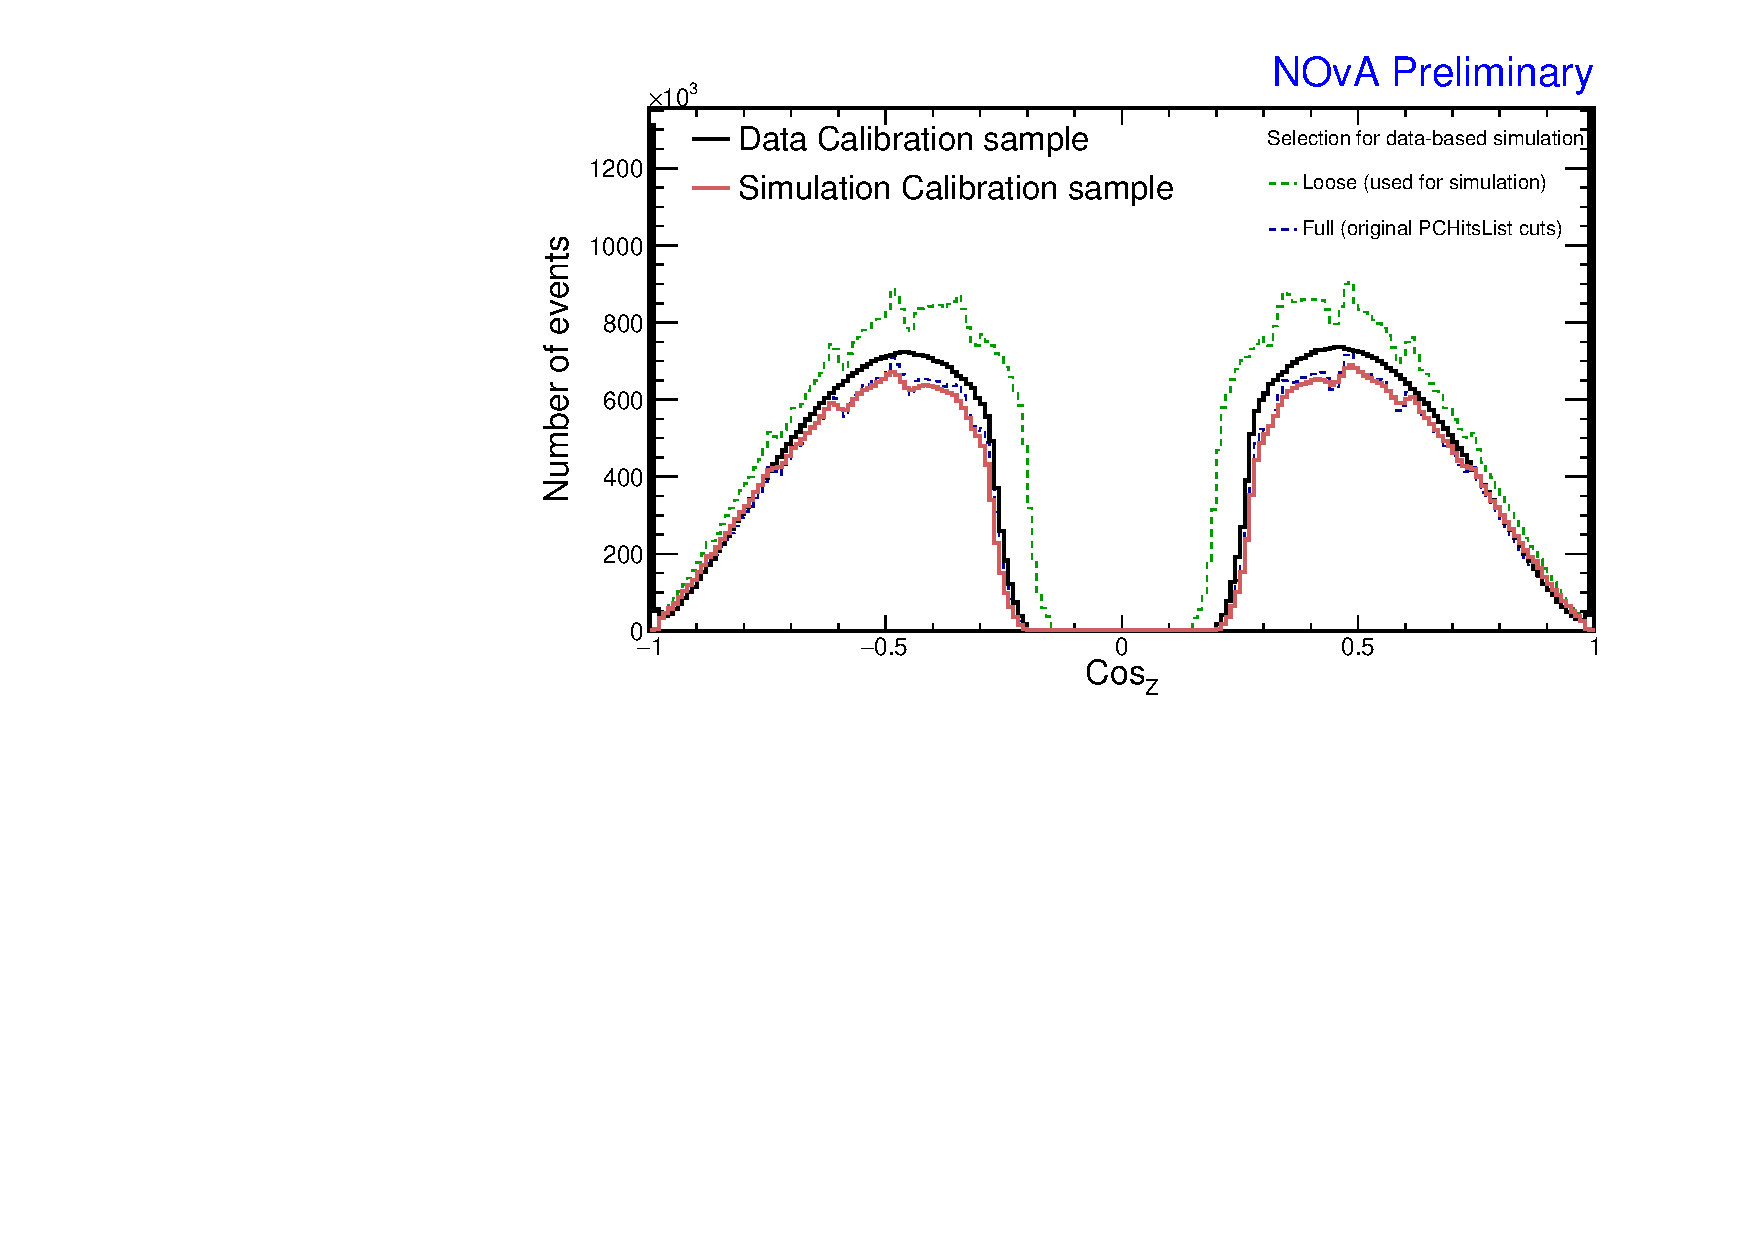
\includegraphics[width=\textwidth]{Plots/TBCalibration/DBSim_DataMCComparison_CosZ.pdf}
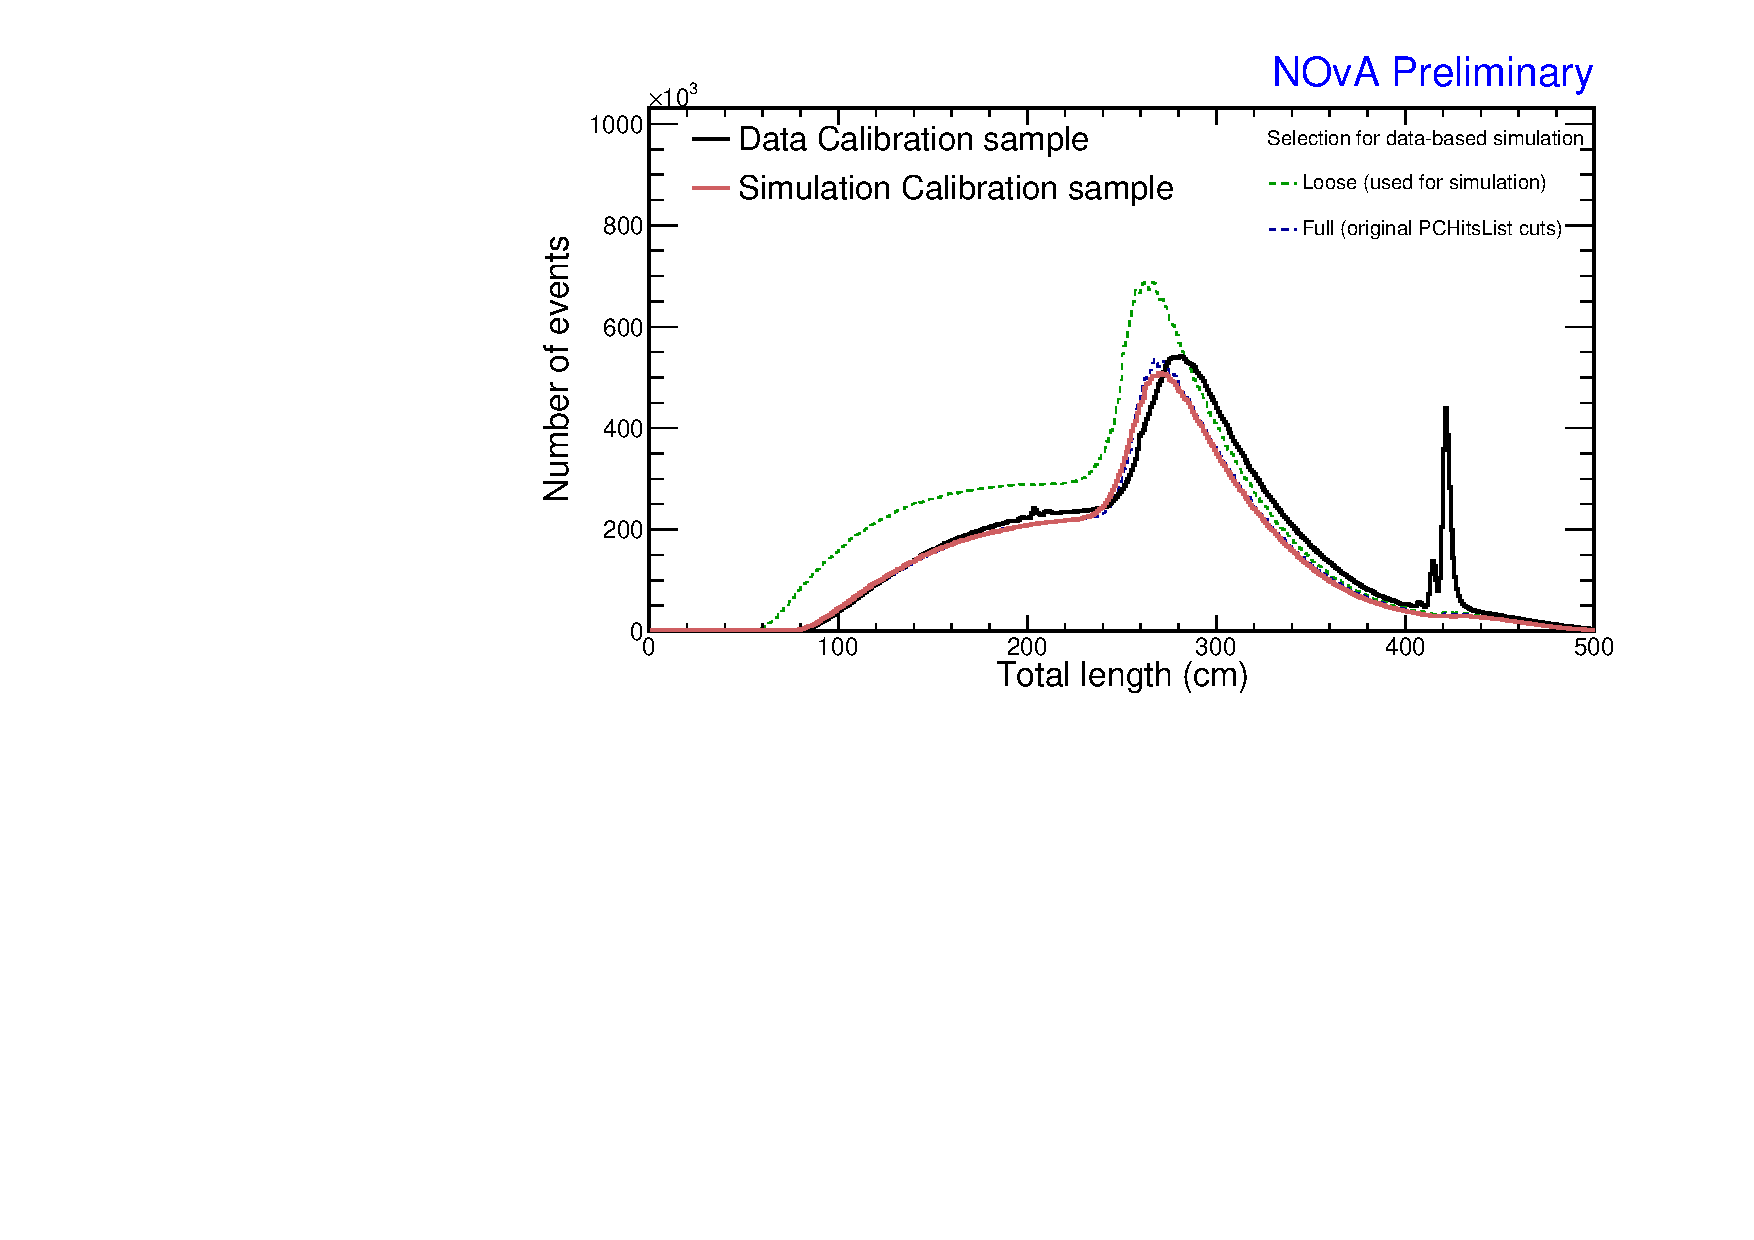
\includegraphics[width=\textwidth]{Plots/TBCalibration/DBSim_DataMCComparison_TotLength.pdf}
\caption[Data-Simulation comparison of angular and track length distributions]{Comparison of the angle from the z axis and total track length between the data (black) and simulation (pink) calibration samples, as detailed in the text. Additionally, the distributions of data with full (blue) and loose (green) selections applied to the \acrshort{BPF} tracks are shown, where the loose selection was used to create the simulation.}
\label{fig:DataBasedSimDataMCComparison_cosZtotLength}
\end{figure}

\begin{figure}[!ht]
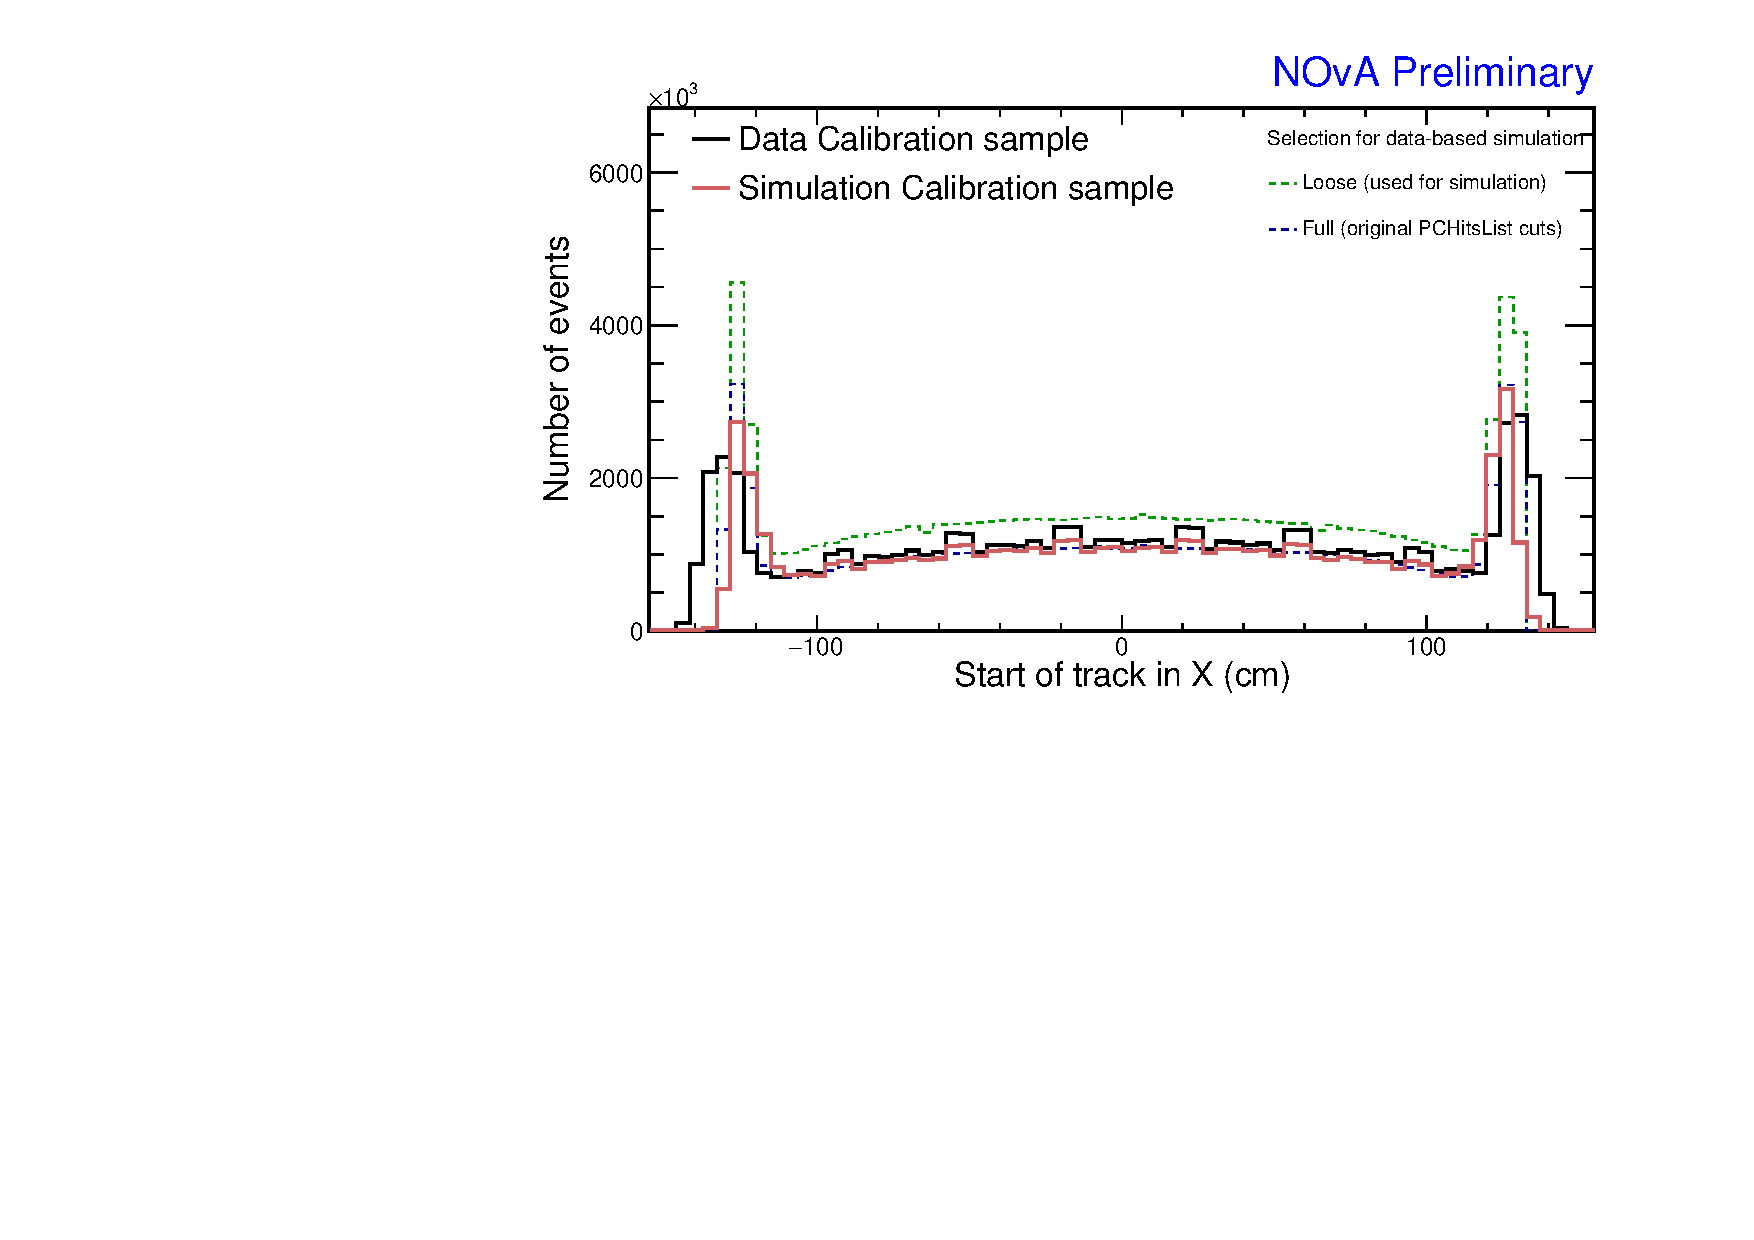
\includegraphics[width=\textwidth]{Plots/TBCalibration/DBSim_DataMCComparison_StartX.pdf}
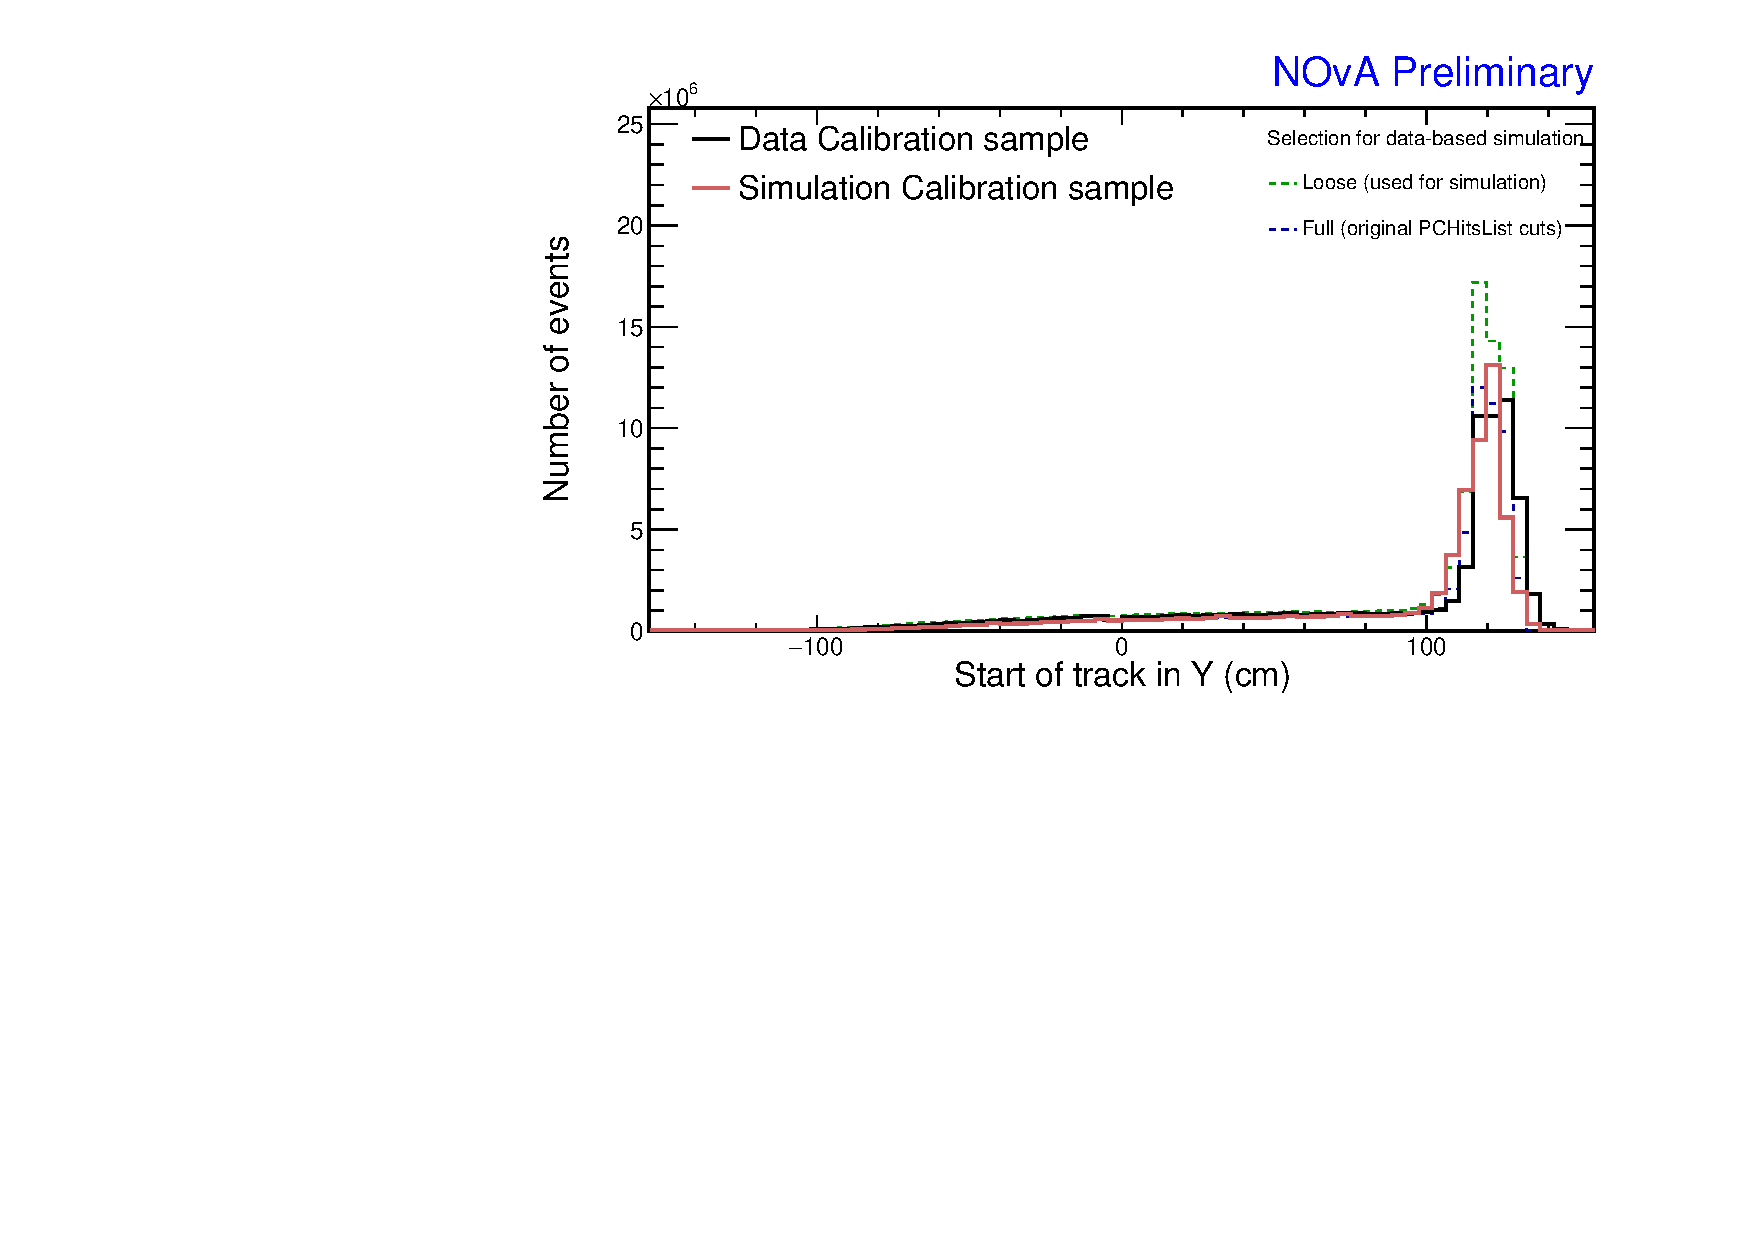
\includegraphics[width=\textwidth]{Plots/TBCalibration/DBSim_DataMCComparison_StartY.pdf}
\caption[Data-Simulation comparison of track start distributions]{Comparison of the x (top) and y (bottom) track start position between the data (black) and simulation (pink) calibration samples, as detailed in the text. Additionally, the distributions of data with full (blue) and loose (green) selections applied to the \acrshort{BPF} tracks are shown, where the loose selection was used to create the simulation.}
\label{fig:DataBasedSimDataMCComparison_startXstartY}
\end{figure}

\begin{figure}[!ht]
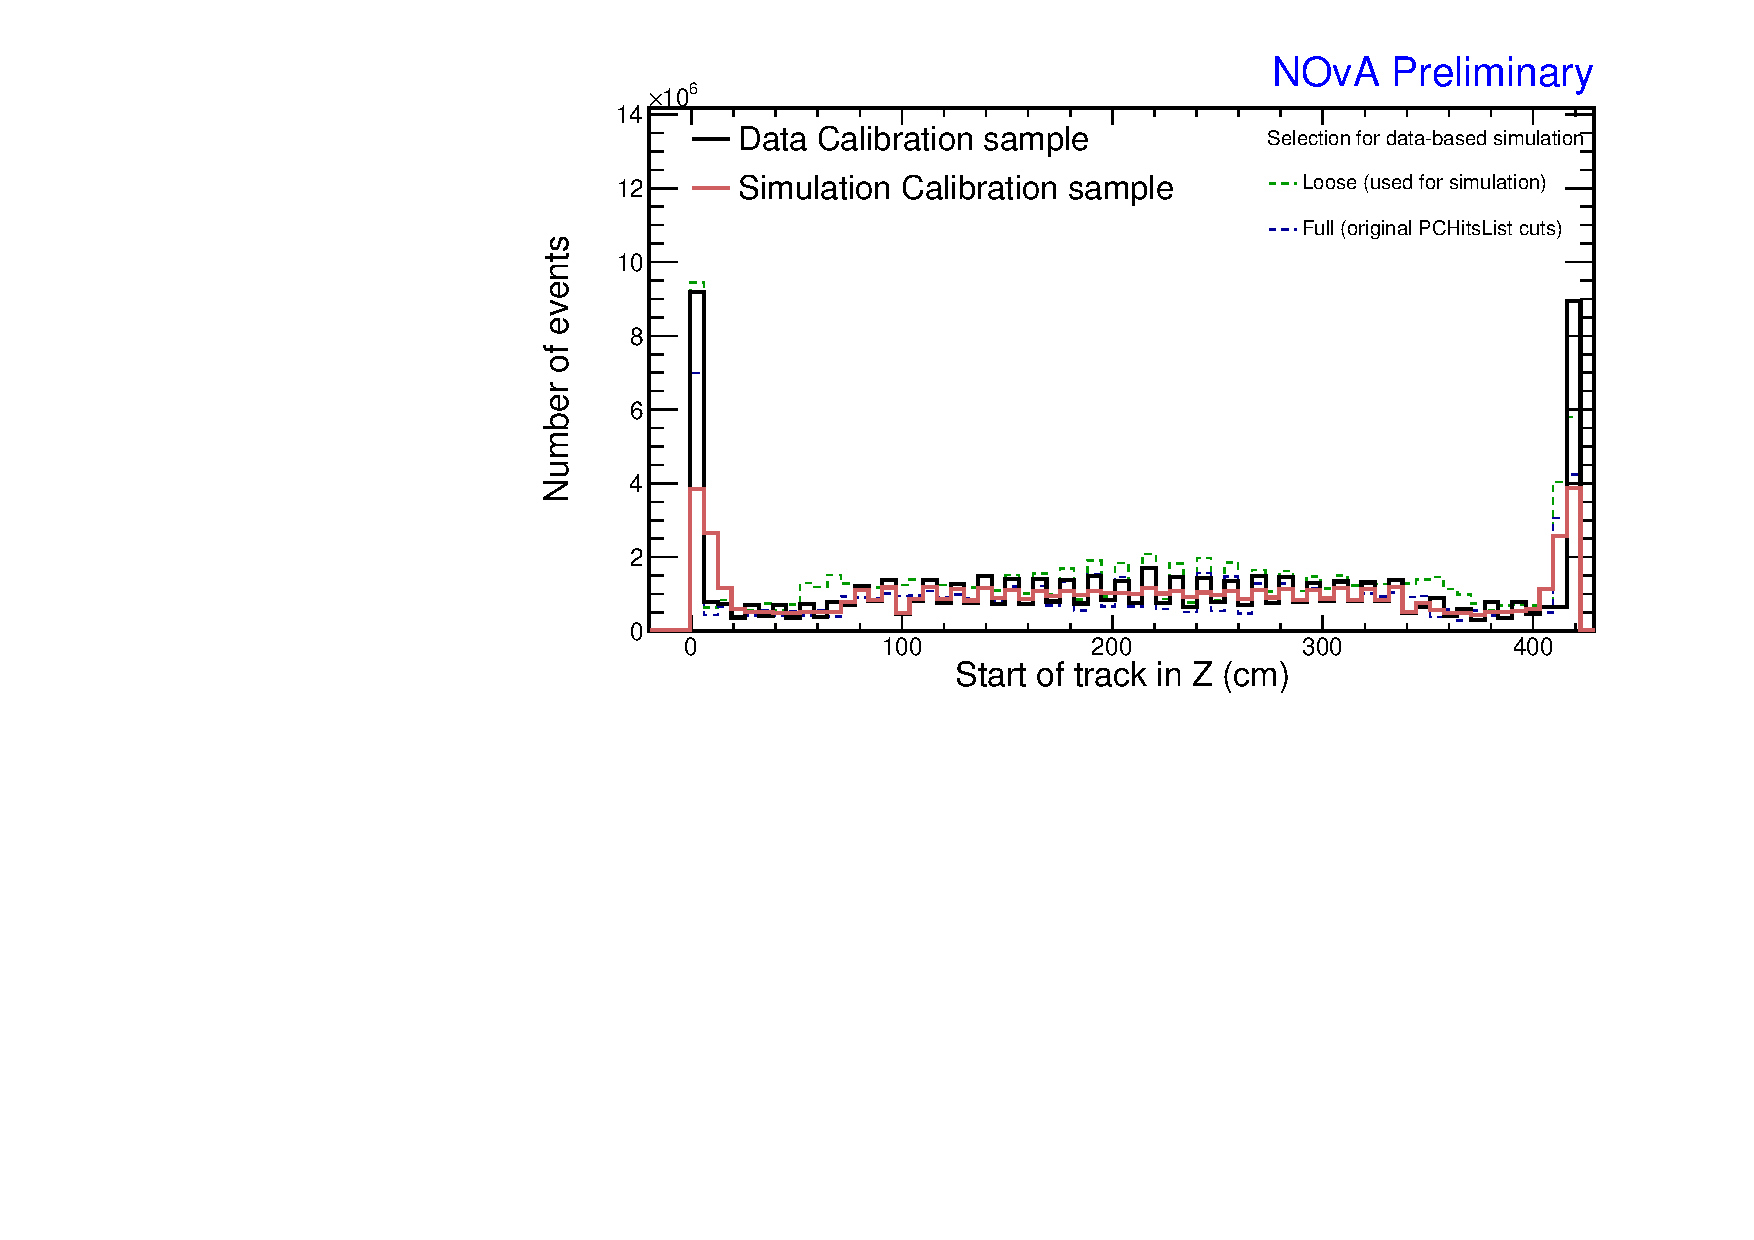
\includegraphics[clip, width=\textwidth]{Plots/TBCalibration/DBSim_DataMCComparison_StartZ.pdf}
\caption[Data-Simulation comparison of track start distribution]{Comparison of the z track start position between the data (black) and simulation (pink) calibration samples, as detailed in the text. Additionally, the distributions of data with full (blue) and loose (green) selections applied to the \acrshort{BPF} tracks are shown, where the loose selection was used to create the simulation. Each bin corresponds to a single detector plane and the shape of the distribution is caused by the fact that cosmic rays are naturally more vertical and therefore more likely to be detected by horizontal than vertical planes.}
\label{fig:DataBasedSimDataMCComparison_startZ}
\end{figure}

%%% Simulation is like the full calibration cuts applied to BPF cuts
It can be seen that the distributions of the new simulation calibration sample resemble those of the data \gls{BPF} tracks with full calibration cuts applied (blue dashed lines) more closely than those of the data calibration sample. This indicates that the simulated window cosmic tracks have similar properties to the data \gls{BPF} tracks, meaning that the differences between the tracking algorithms have an impact on the resulting simulation. Therefore, loosening the calibration cuts did not help with mitigating these differences as expected. However, there were in total four versions of simulation created, with varying event selections and smearing applied, including using full calibration cuts and with different loosened calibration cut values. It is clear that it is unlikely we can mitigate the differences between the window cosmic tracks and the \gls{BPF} tracks simply by changing the event selection or smearing and it would require adapting (or developing) a different reconstruction algorithm for the simulation. Due to the time and effort required for such a task, and due to the relative similarity between the simulation and data calibration samples, we decided to proceed with the reconstruction, selection, and correction as described above.

%%% Beam-like data removed (refer back to selection)
Figures~\ref{fig:DataBasedSimDataMCComparison_cosXcosY} and \ref{fig:DataBasedSimDataMCComparison_cosZtotLength} show the effect of removing the beam-like events with a $\left|\textsf{Cos}_Z\right|<0.98$ cut as described in Sec.~\ref{sec:DataBasedSimSelection}.  While we applied this cut to the data events used to create the simulation (green dashed lines), it is not included in the selection process for the calibration samples. This means that we were successful in removing these undesirable events from the new simulation. This can be seen by the wide peaks at $\textsf{Cos}_{X/Y}=0$ in Fig.~\ref{fig:DataBasedSimDataMCComparison_cosXcosY} which are present for the data calibration sample, by not for the simulation. Additionally, sharp peaks in the total track length and in the edges of the angle from the z axis distributions in Fig.~\ref{fig:DataBasedSimDataMCComparison_cosZtotLength} further illustrate this distinction.
%The wide peaks at $\textsf{Cos}_{X/Y}=0$ correspond to tracks parallel to the z axis, which are likely leftover beam events that were removed for simulation (Sec.~\ref{sec:DataBasedSimSelection}, but not in data.
%The simulation calibration sample has an additional cut on $\left|\textsf{Cos}_Z\right|<0.98$ that removes beam-like events (Sec.~\ref{sec:DataBasedSimSelection}) compared to data. This can be clearly seen on the top plot with peaks on the left and right sides if the data calibration sample's distribution, which are removed for in simulation. It can also be seen in the bottom plot, where the removed beam-like events correspond to the peaks around $\unit[200]{cm}$ and $\unit[420]{cm}$.

%%% Rugged shape helped a little by smearing
The effect of smearing of vertex positions and four momenta is visible in the top plot of Fig.~\ref{fig:DataBasedSimDataMCComparison_cosZtotLength} and in Fig.~\ref{fig:DataBasedSimDataMCComparison_startZ}. Here, the rugged distributions of the data used for simulation (green dashed lines) appears smoother for the simulation calibration sample (pink solid lines). However, comparisons of track start positions in Fig.~\ref{fig:DataBasedSimDataMCComparison_startXstartY} and \ref{fig:DataBasedSimDataMCComparison_startZ} show that the simulated events start further away from the detector edge compared to data. While this is likely also a result of smearing, we anticipate it will not impact the calibration of the simulated detector.
% The simulation calibration sample has a smaller differences between the horizontal and vertical planes, presumably due to the smearing applied (Sec~\ref{sec:DataBasedSimPython}).

%%% Smearing (or reco?) caused events to start more inside of the detector
%The start of track comparison between data and simulation in Fig.~\ref{fig:DataBasedSimDataMCComparison_startXstartY} and \ref{fig:DataBasedSimDataMCComparison_startZ} show that there are fewer events that start at the edge of the detector and the vertex positions are moved slightly towards the inside of the detector. This is likely the result of the smearing of the vertex positions and we do not expect this to have an effect on the calibration. 

%%% Adding re-simulation samples
After adding the distributions for the re-simulation calibration sample, shown as solid brown lines Fig.~\ref{fig:DataBasedSimSimVersionComparison}, we can see that the track start positions are shifted even further towards the inside of the detector. This would support the hypothesis that this effect is caused by smearing and is also likely related to the loss of events with longer track lengths, as shown in Fig.~\ref{fig:DataBasedSimSimVersionComparison}, since if tracks start a few centimetres later in the detector their tracks would get shorter by the same amount. Since there are only minimal discrepancies between the simulation and the re-simulation, we conclude that the reconstruction, selection and correction processes used to create the simulation do not significantly bias the simulation, which is self-consistent.

\begin{figure}[!ht]
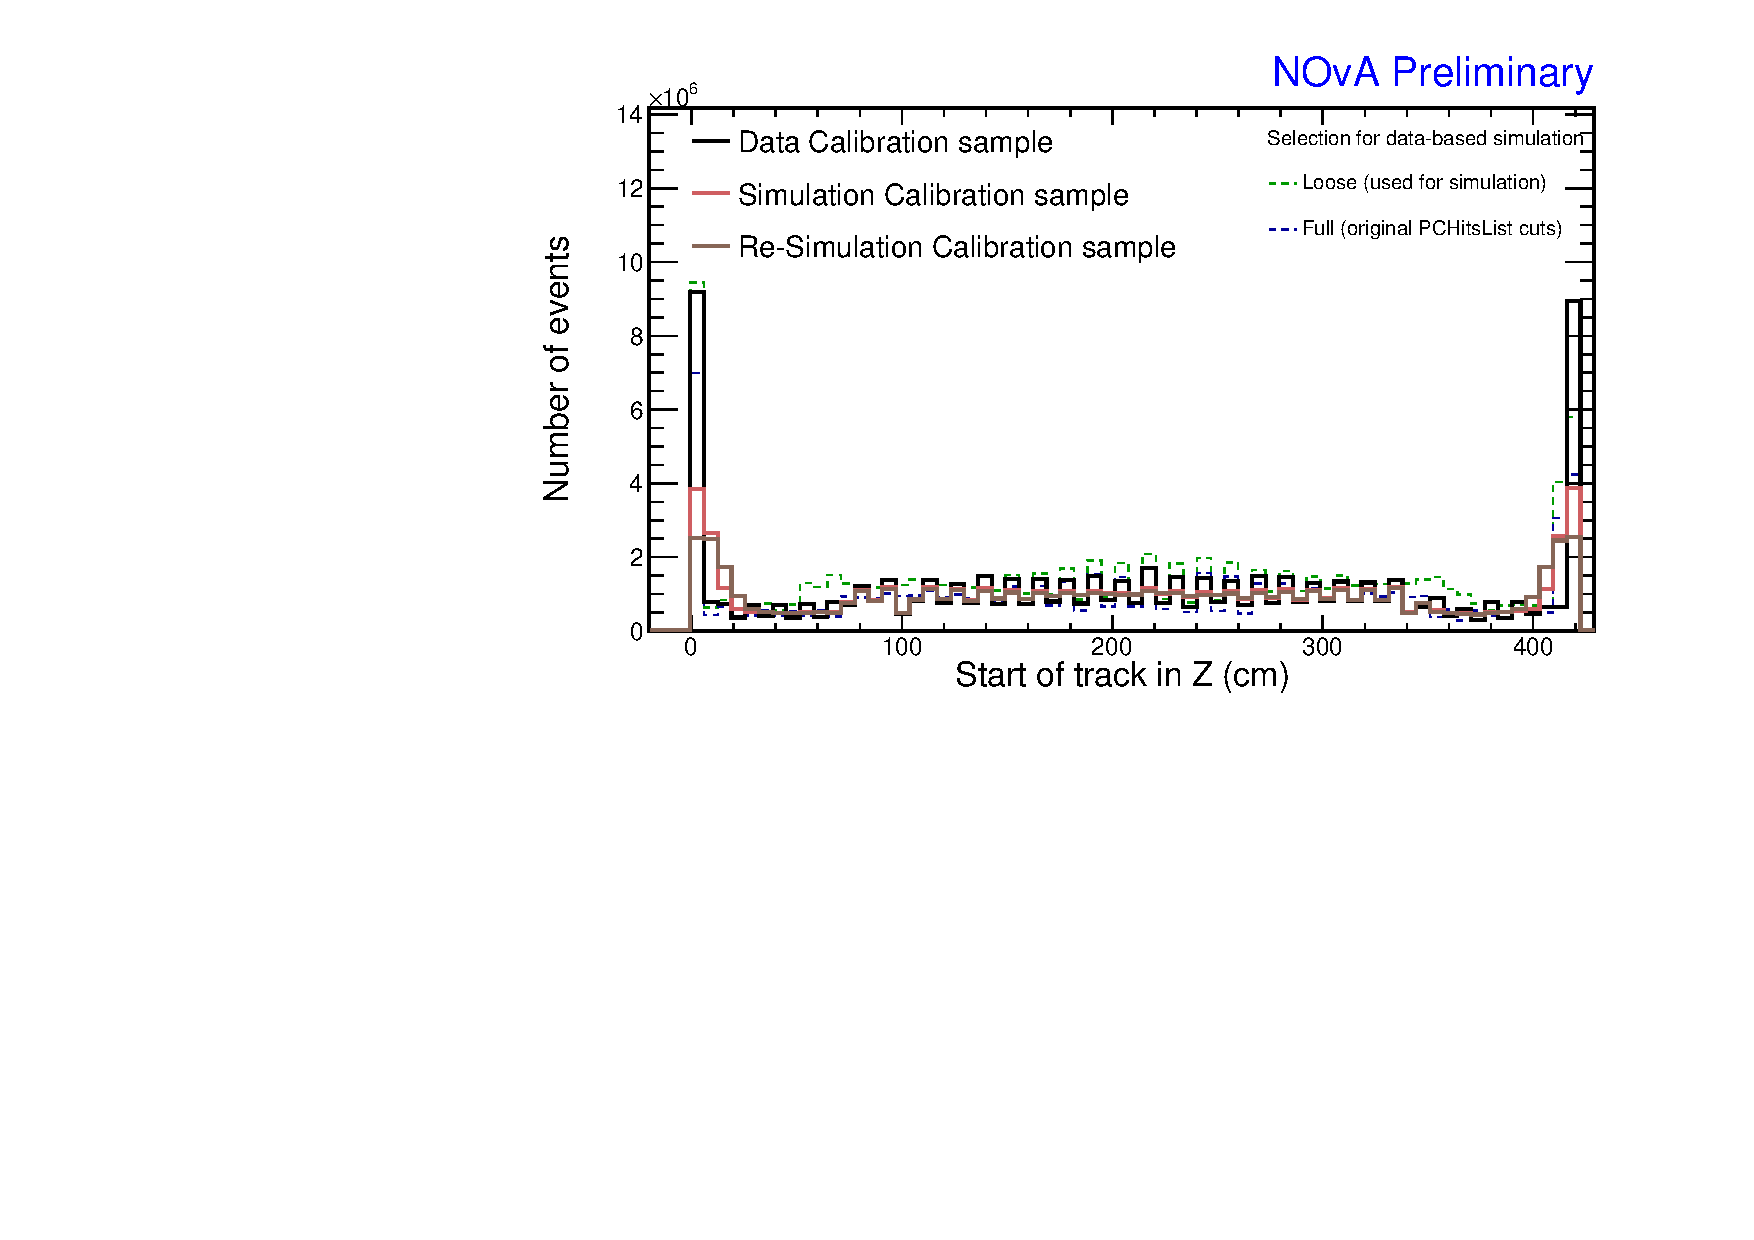
\includegraphics[width=\textwidth]{Plots/TBCalibration/DBSim_SimVersionComparison_StartZ.pdf}
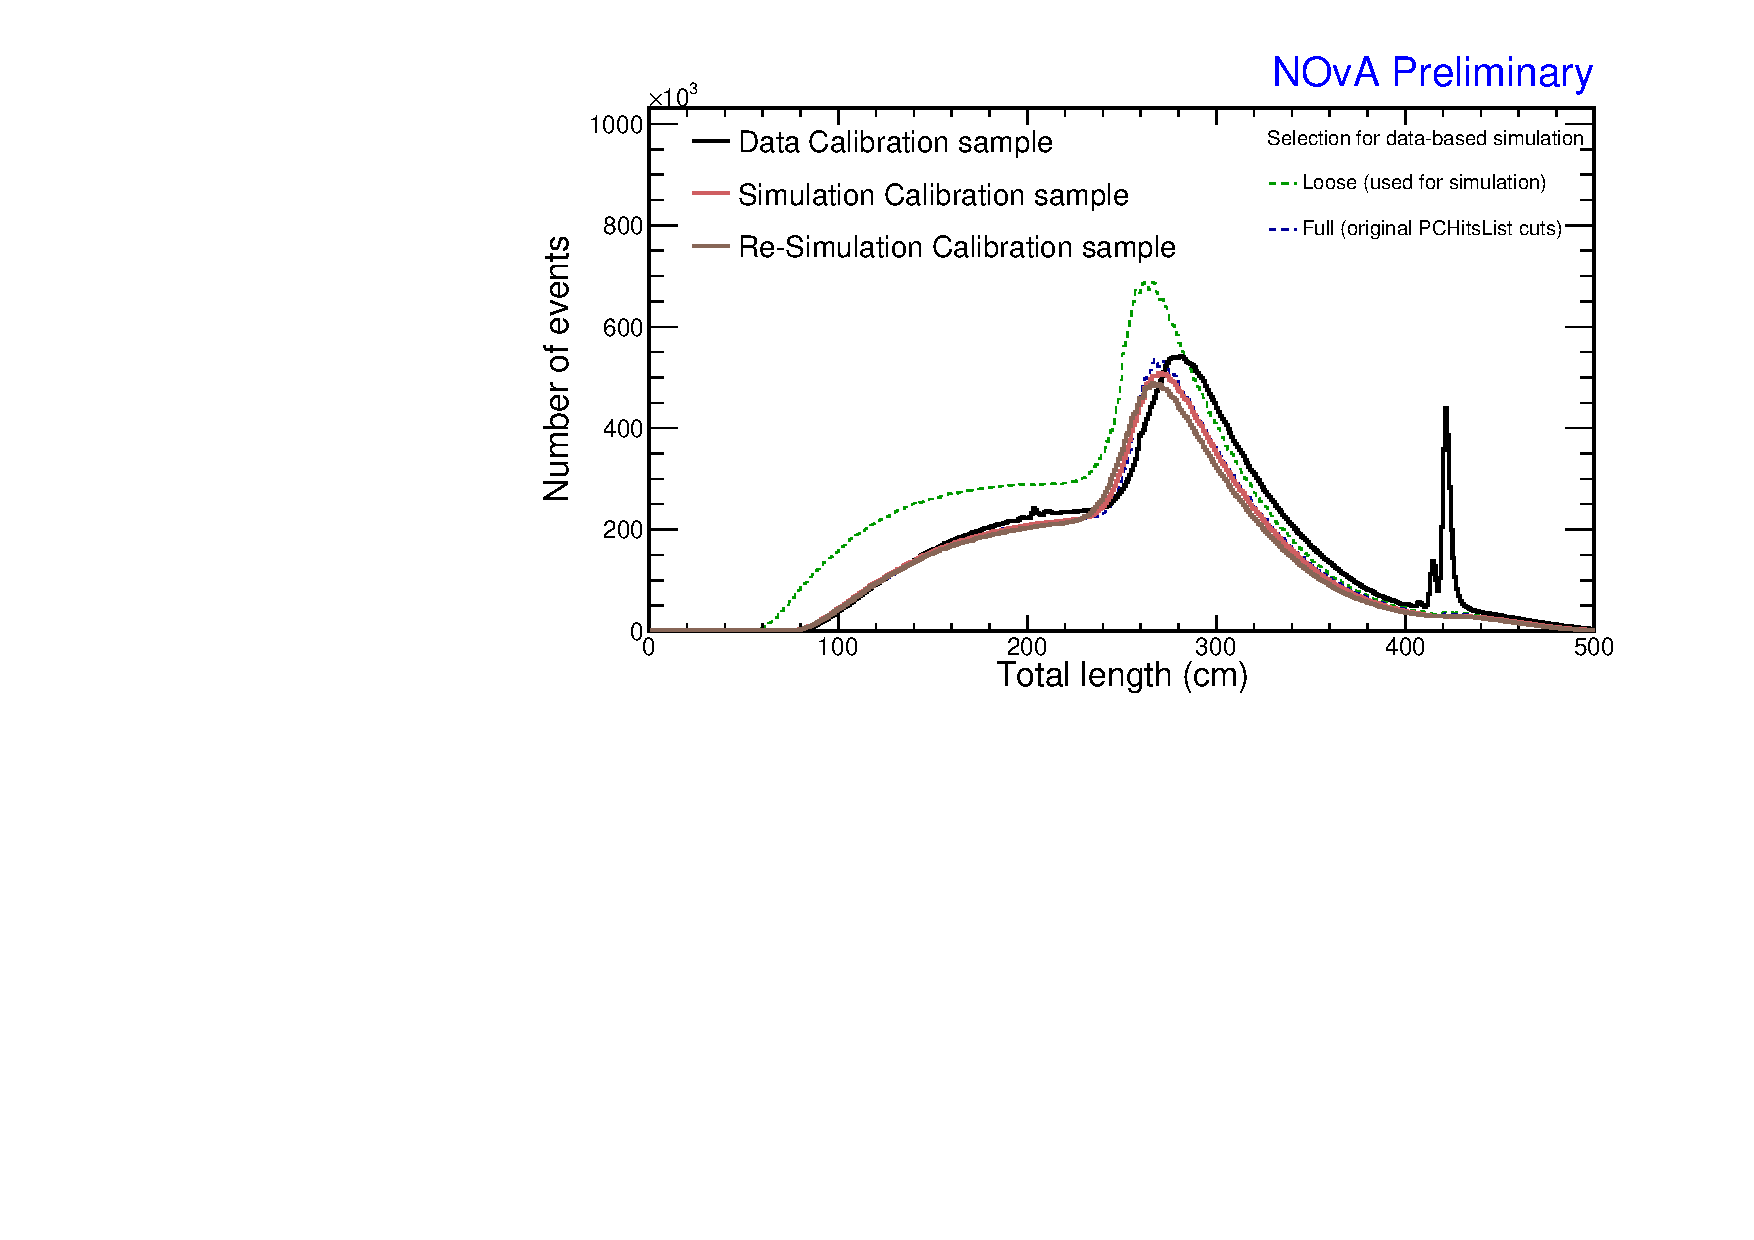
\includegraphics[width=\textwidth]{Plots/TBCalibration/DBSim_SimVersionComparison_TotLength.pdf}
\caption[Comparison of simulation to a re-simulation validation sample]{Comparison of the z track start position and total track length between the re-simulated events (brown), which use simulation as `fake data' for the second iteration of the same simulation process, and the data (black) and simulation (pink) events. Additionally, the distributions of data with full (blue) and loose (green) selections applied to the \acrshort{BPF} tracks are shown, where the loose selection was used to create the simulation.}
\label{fig:DataBasedSimSimVersionComparison}
\end{figure}

\subsection{Conclusion}
\note{Should I include this conclusion section here?}

I have successfully developed a new simulation of cosmic muons intended for Test Beam calibration. The reconstruction, selection, and correction processes were designed to minimize the number of simulated events, resulting in an efficient and concise simulation while avoiding a significant bias, particularly in the applicability to the calibration procedures.

While the simulation achieved its objectives, there are possible improvements that could be introduced to refine it. Using a different track reconstruction algorithm than the \gls{BPF} more consistent with the window cosmic track algorithm could make the simulation calibration sample more alike the data calibration sample. Additionally, developing a more sophisticated energy correction procedure, potentially involving external measurements of energy distribution of cosmic muons, would enable simulation of through-going muons with accurate incident energies.

Looking ahead, there are plans to use the data-based simulation approach for cosmic muons in the \gls{NOvA} \gls{ND} and \gls{FD}. While the primary motivation is again detector calibration, there is potential for broader applications in cosmic ray studies. However, using the simulation for a different detector would require re-validating the event selection process, especially with the inclusion of the calibration cuts missing for the Test Beam detector, as outline in Sec.~\ref{sec:DataBasedSimSelection} and showed shaded out in two bottom rows of Tab.~\ref{tab:DataBasedSimEventSelection}.

%%%%%%%%%%%%%%%%%%%%%%%%%%%%%%%%%%%%%%%%%%%%%%%%%%%%%%%%%%%%%%%%%%%%%%%%%%%%%%%
%%%%%%%%%%%%%%%%%%%%%%%%%%%%%%%%%%%%%%%%%%%%%%%%%%%%%%%%%%%%%%%%%%%%%%%%%%%%%%%
%%%
%%%                      Test Beam calibration description
%%%
%%%%%%%%%%%%%%%%%%%%%%%%%%%%%%%%%%%%%%%%%%%%%%%%%%%%%%%%%%%%%%%%%%%%%%%%%%%%%%%
\section{NOvA Test Beam Detector Calibration}\label{sec:TBCalibrationSection}
In this section I describe the details of the Test Beam detector calibration as it was finalized in June 2023. This version includes a new purpose-made simulation and all the measured Test Beam data, with the exception of the period 1 data.

The data calibration samples for Test Beam were created using the same procedures as the \gls{ND} and \gls{FD} calibration samples, described in Sec.~\ref{sec:NOvACalibration}. However, there are two cuts from the event election, that were not included for Test Beam during the processing of the data samples. This can be seen on Tab.~\ref{tab:DataBasedSimEventSelection}, where the two bottom rows show the two excluded cuts. One cut contains the vertex close to the edge of the detector ensuring we only use cosmic events, the other contains the end of track close to the edge, ensuring we only use through-going muons for the relative calibration. Given that we remove beam events and that all the other cuts are designed to select cosmic events, the first cut has only a negligible effect on the final selection. Additionally, the stopping muons only make up a small fraction of the total cosmic muon events, rendering the second cut also negligible.

This section is organized as follows. I first describe the Test Beam versions of the fibre brightness map in Sec.~\ref{sec:FibreBrightnessTB} and the threshold and shielding correction in Sec.~\ref{sec:TBThresholdCorrection}, as they were introduced in Sec.~\ref{sec:NOvACalibration}. I then go over the simulation sample and the three data samples (for periods 2, 3, and 4), showing distributions of hits selected for calibration and of the uncorrected energy deposition before calibration. I discuss considerations going into calibration, including splitting the individual periods into smaller samples, or describing issues that could affect the calibration results.  Afterwards, I am showing a selection of attenuation fit results for each sample together with an overview of the relative calibration effects. Lastly, I discuss the absolute calibration results for all the samples combined, as well as the validation and conclusion of the Test Beam calibration.

%Temperature study (small overview - probably not needed at all, depends if Randeeth want to add his work to this technote)

%From Teresa's thesis
%Along with setting the energy scale of the detector, we need to calibrate the timing of the readout system for the detector. The Data Concentrator Modules (DCMs) responsible for collating the data from multiple FEBs get their timing information via a daisy chain originating at the detector TDU. Each DCM in the chain has a timing offset relative to the DCM before it, with the last DCM having the earliest ti. Following the procedure described in [66], I used timing information from hits on cosmic ray muon tracks that pass through multiple DCMs to determine the relative offsets between DCMs, shown in Figure 3.20.

%From Teresa's thesis:
%"For Test Beam, we have three beam-based triggers, one pulsed trigger, and two data-driven triggers. The data-driven triggers are both activity-based triggers. The first is intended to record cosmic ray induced events for use in calibrating the detector.

\subsection{Fibre Brightness}\label{sec:FibreBrightnessTB}

To divide the Test Beam detector into \gls{FB} bins we use the attenuation fit results for Test Beam period 4 data (described in Sec.~\ref{sec:TBPeriod4}), as that is the best detector conditions data we have. Since we need the \gls{FB} map in order to run the attenuation fits and we need the attenuation fit results to create the \gls{FB} map, we proceeded iteratively. We first run the attenuation fit with an older version of the \gls{FB} map and use the results to create a new \gls{FB} map, discussed here, which is then used in a new attenuation fit.

We are only using the attenuation fit results in the centre of each cell to create the \gls{FB} map, therefore, we decided to allow some cells that failed the calibration condition ($\chi^2>0.2$), to be still used for the creation of the \gls{FB} map. Otherwise, all the officially uncalibrated cells are assigned an average response across the entire detector, resulting in a loss of information on their relative brightness. As can be seen in Fig.~\ref{fig:FiberBrightnessExamples}, some attenuation fits have $\chi^2>0.2$, even though they correctly represent the energy deposition in the centre of that cell. By carefully investigating all the uncalibrated Test Beam cells (doable for Test Beam, due to its small number of cells), we concluded that all the cells with $\chi^2<0.7$ can be used to create the \gls{FB} map, since the response in their centre is described reasonably well by their attenuation fits. We use this loosened calibration condition only to create the \gls{FB} map and we keep the original condition for the actual calibration results.

%Describe and show plots that since we are only using the fitted response at cell centre we can allow fits with $\chi^2>0.2$. Show examples of responses with chisq larger than that and say what is the final chisq chosen. No need to show the final distribution of the fb bins here as they were technically shown in the general calibration description. But might refer back to it...

\begin{figure}[h]
\centering
\begin{subfigure}[b]{0.495\textwidth}
\centering
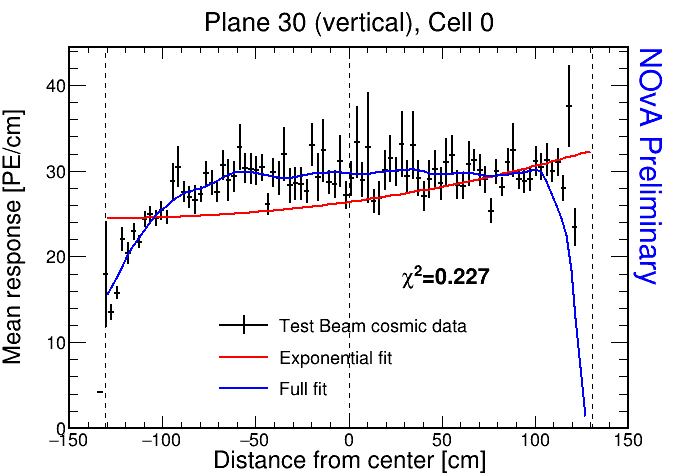
\includegraphics[width=\textwidth]{Plots/TBCalibration/ExampleForBrightFile_fb0_030_000.png}
\end{subfigure}
%\hfill
\begin{subfigure}[b]{0.495\textwidth}
\centering
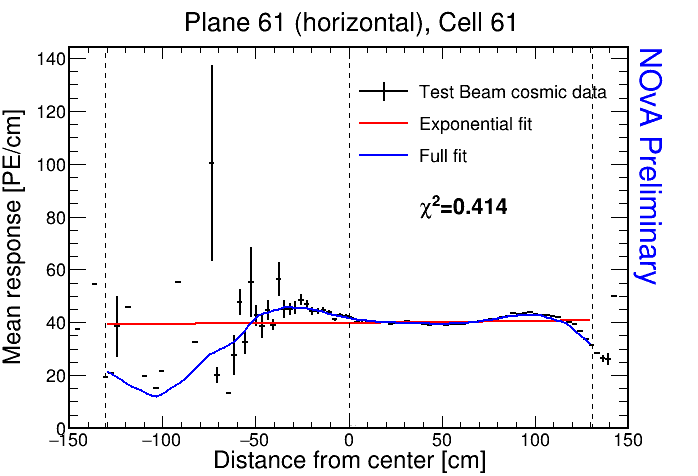
\includegraphics[width=\textwidth]{Plots/TBCalibration/ExampleForBrightFile_fb5_061_061.png}
\end{subfigure}
\caption[Example of failed attenuation fits used for the Test Beam fibre brightness file]{Examples of attenuation fits for two cells that fail the calibration condition, but the fit (blue line) still correctly represents the energy deposition in the centre of that cell (dashed vertical line in the middle). The total $\chi^2$ between the data (black) and the attenuation fit for both plots are included.}
\label{fig:FiberBrightnessExamples}
\end{figure}

The final distribution of relative \gls{FB} values that are used to populate the \gls{FB} bins for the Test Beam detector is shown in Fig.~\ref{fig:TBFiberBrightnessMap}. The resulting map of \gls{FB} bins and their corresponding relative brightnesses was shown in the previous chapter in Fig.~\ref{fig:NOvAFiberBrightness}.

\begin{figure}[hbtp]
\centering
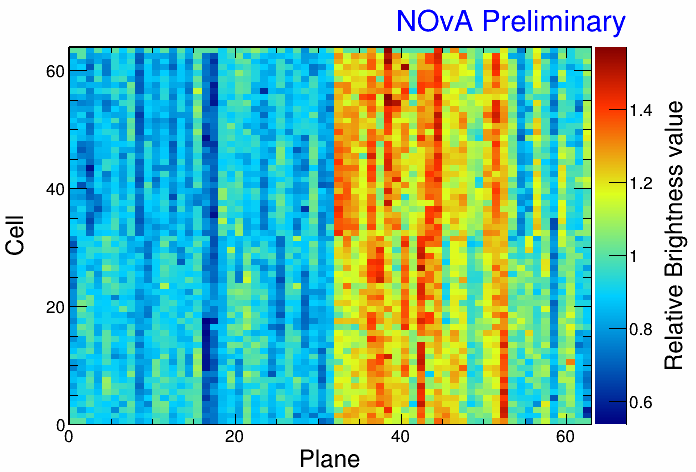
\includegraphics[width=.8\textwidth]{Plots/TBCalibration/TBFiberBrightnessMap.png}
\caption[Fibre Brightness map for the Test Beam detector]{\acrshort{FB} map representing relative differences in energy response due to different brightnesses of the fibres, scintillators, or readout. Create from the attenuation fit results of the \acrshort{NOvA} Test Beam detector with a shifted calibration condition from $\chi^2<0.2\rightarrow 0.7$ to enable using the attenuation fits that are officially uncalibrated, but correctly represent energy deposition in cell centre. Otherwise, all the uncalibrated cells get assigned a mean detector response, represented by number 1 on this map.}
\label{fig:TBFiberBrightnessMap}
\end{figure}

\subsection{Threshold and Shielding Corrections}\label{sec:TBThresholdCorrection}
%Describe in generall what is TS correction for
The threshold and shielding correction is intended to mitigate biases arising from differences between cosmic events used for calibration and beam events. It is only used prior to the attenuation fits and is omitted when applying the results of the relative calibration, whether during the absolute calibration or for beam events. Additionally, it is derived exclusively from simulation.

%TS correction dependence on w
We created a new threshold and shielding correction for the Test Beam detector using the new simulation described in Sec.~\ref{sec:DataBasedSimulation}. The correction is calculated for both views, across 12 \gls{FB} bins, 64 cells, and 100 $w$ bins, where $w\in\left(\unit[-130]{cm},\unit[130]{cm}\right)$. Two examples of the correction as a function of $w$ are shown in Fig.~\ref{fig:TBThresholdCorrectionExamples}, demonstrating an almost uniform behaviour along a cell. Relative variations of the correction in the X view range from $\unit[1-2]{\%}$,  primarily concentrated at the edges of the cell. In the Y view, the correction exhibits sub-$\unit[1]{\%}$ variations. These trends are consistent across all the \gls{FB} bins and views. Given that the threshold and shielding correction precedes relative calibration, the absolute value of the correction is irrelevant and only the relative variations along $w$ and between cells matter.
 
\begin{figure}[!hbtp]
\centering
\begin{subfigure}[t]{\textwidth}
\centering
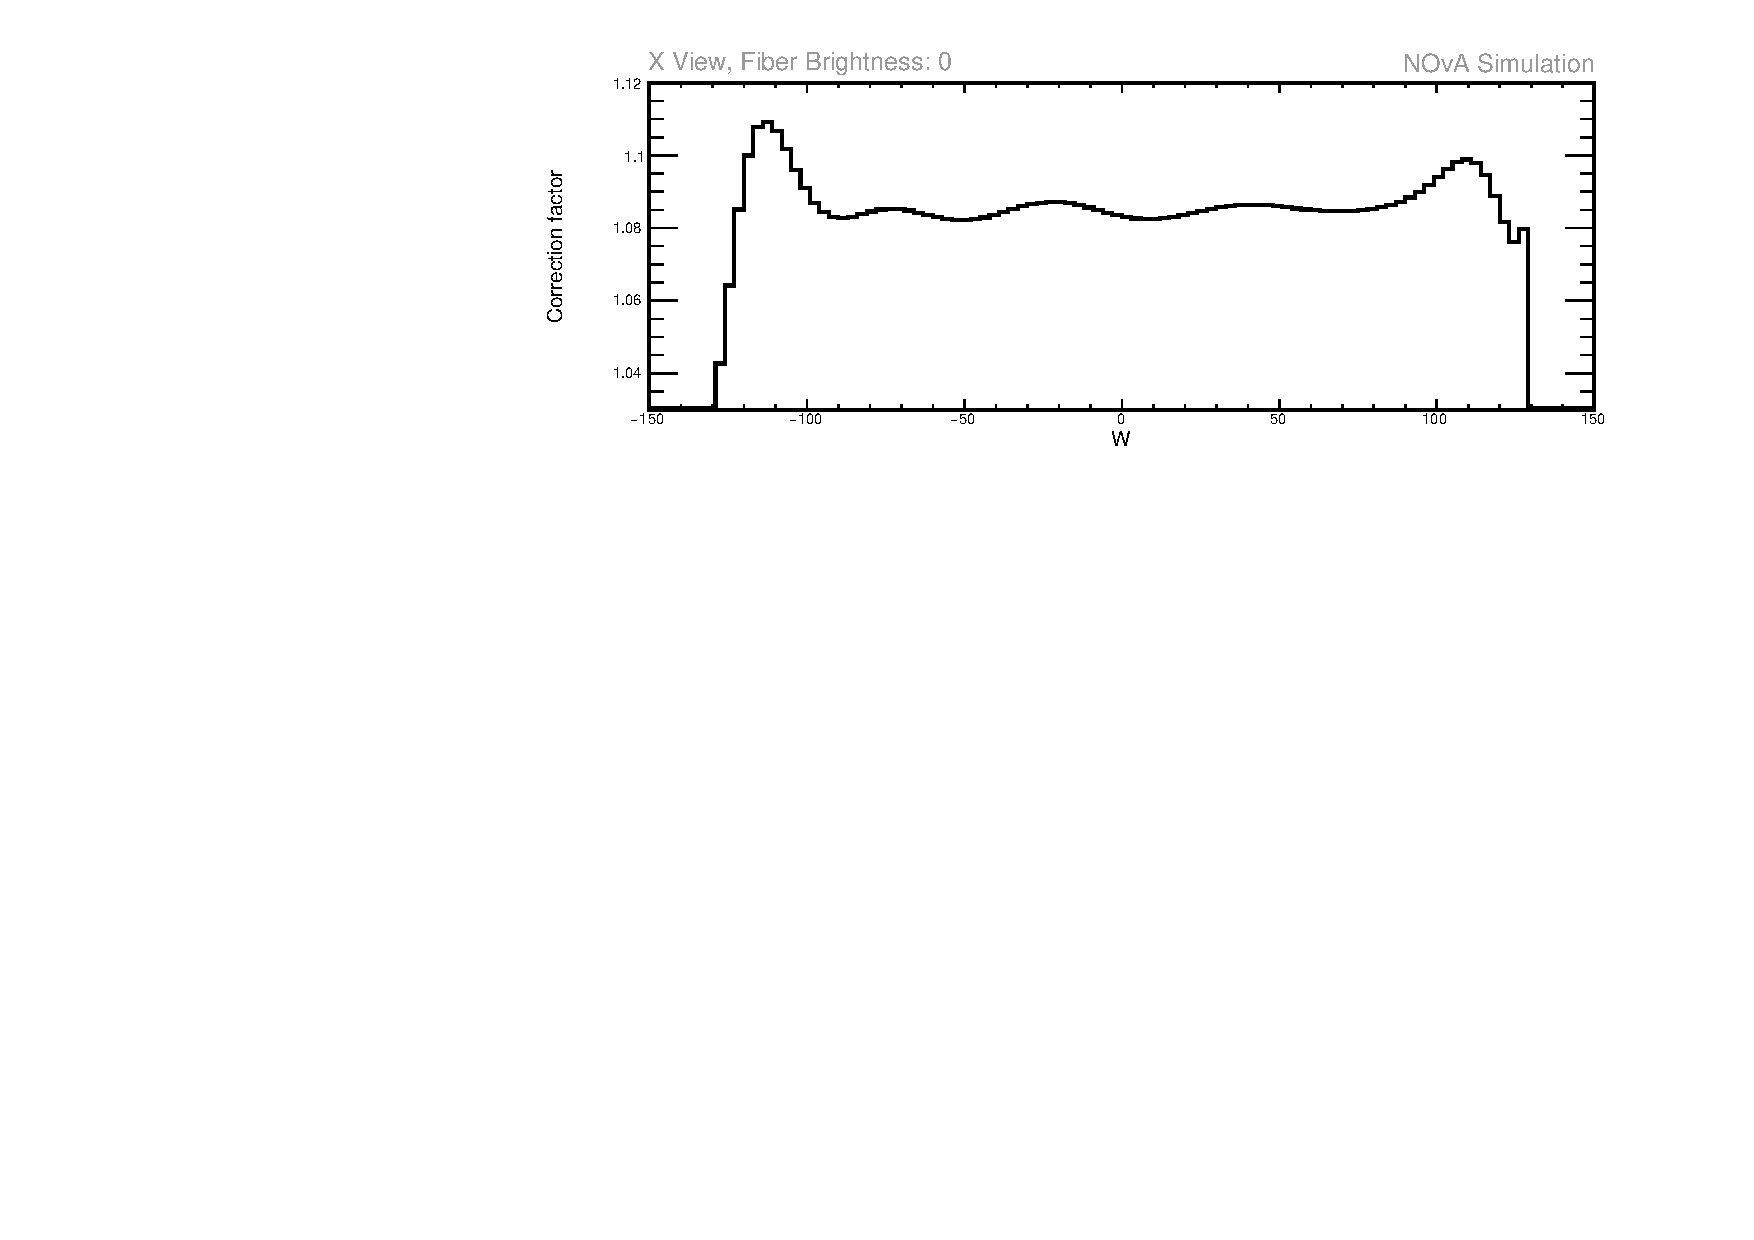
\includegraphics[width=\textwidth]{Plots/TBCalibration/ThresholdCorrectionExample_axview_fb0_P4DataBasedSim.pdf}
\end{subfigure}
\begin{subfigure}[b]{\textwidth}
\centering
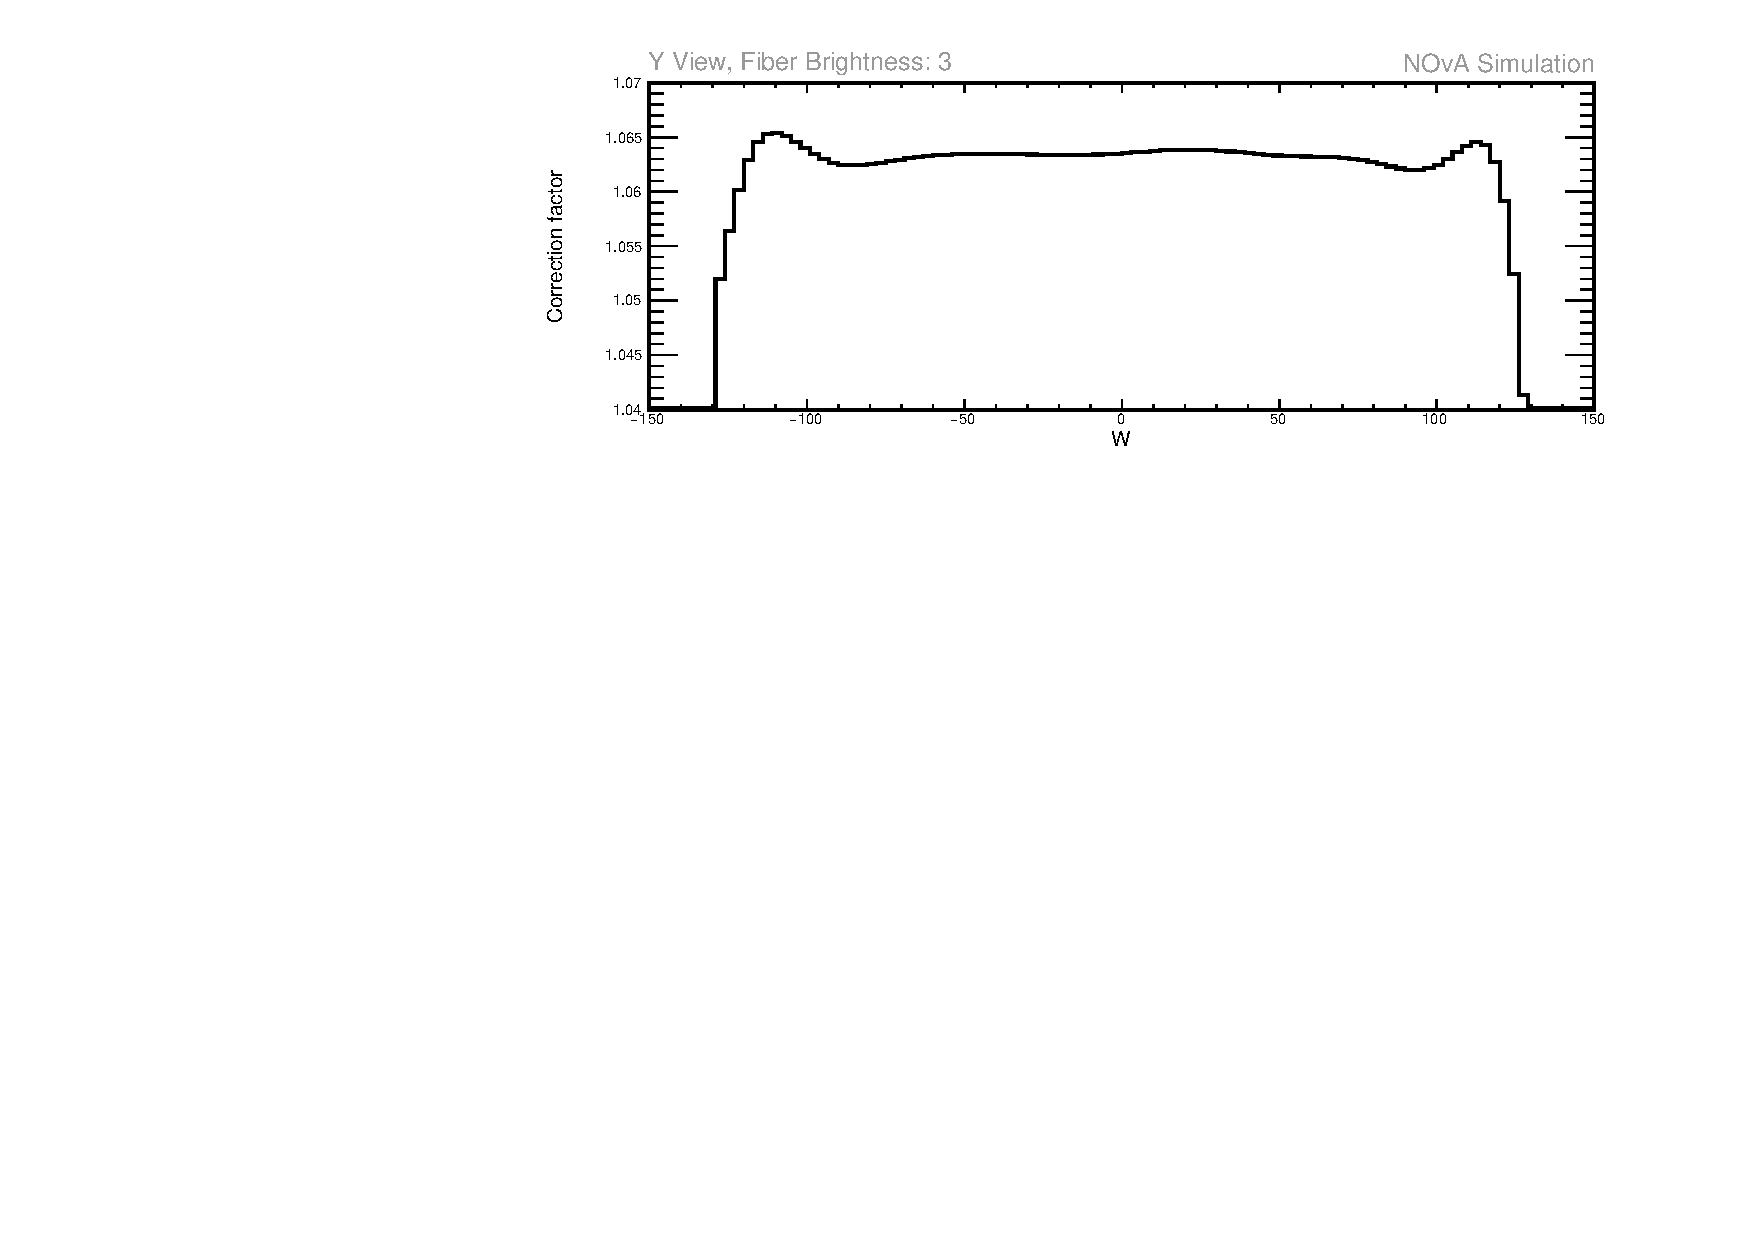
\includegraphics[width=\textwidth]{Plots/TBCalibration/ThresholdCorrectionExample_ayview_fb3_P4DataBasedSim.pdf}
\end{subfigure}
\caption{Examples of threshold and shielding corrections as a function of the position within a cell in X view (top) and Y view (bottom) for the Test Beam detector.}
\label{fig:TBThresholdCorrectionExamples}
\end{figure}

%Where do the variations come from?
This uniformity of the distributions is expected, considering the relatively small size of the Test Beam detector compared to the \gls{FD}, which prompted the investigation into threshold and shielding effects. The Test Beam detector's cell length of $\unit[2.6]{m}$ has only a negligible impact on the threshold saturation or on the energy distribution of cosmic muons, resulting in  the uniformity of the threshold and shielding correction for Test Beam detector. The larger correction at cell edges is likely caused by lower event counts in those areas. However, since this relative sparsity of events also influences relative calibration due to large variation in the energy response, the relatively larger threshold and shielding correction at cell edges is not detrimental.

%Dependence of the TS correction on plane and cell
The distribution of the threshold and shielding correction across Test Beam detector's cells and planes, shown in the top of Fig.~\ref{fig:TBThresholdCorrectionMap}, demonstrates, that while the correction is expected to be generally uniform across the detector, there are notable variations between cells and planes forming a discernible pattern. These variations and their shape primarily stem from the threshold component of the correction, shown in the bottom of Fig.~\ref{fig:TBThresholdCorrectionMap}.

\begin{figure}[!hbtp]
\centering
\begin{subfigure}[t]{\textwidth}
\centering
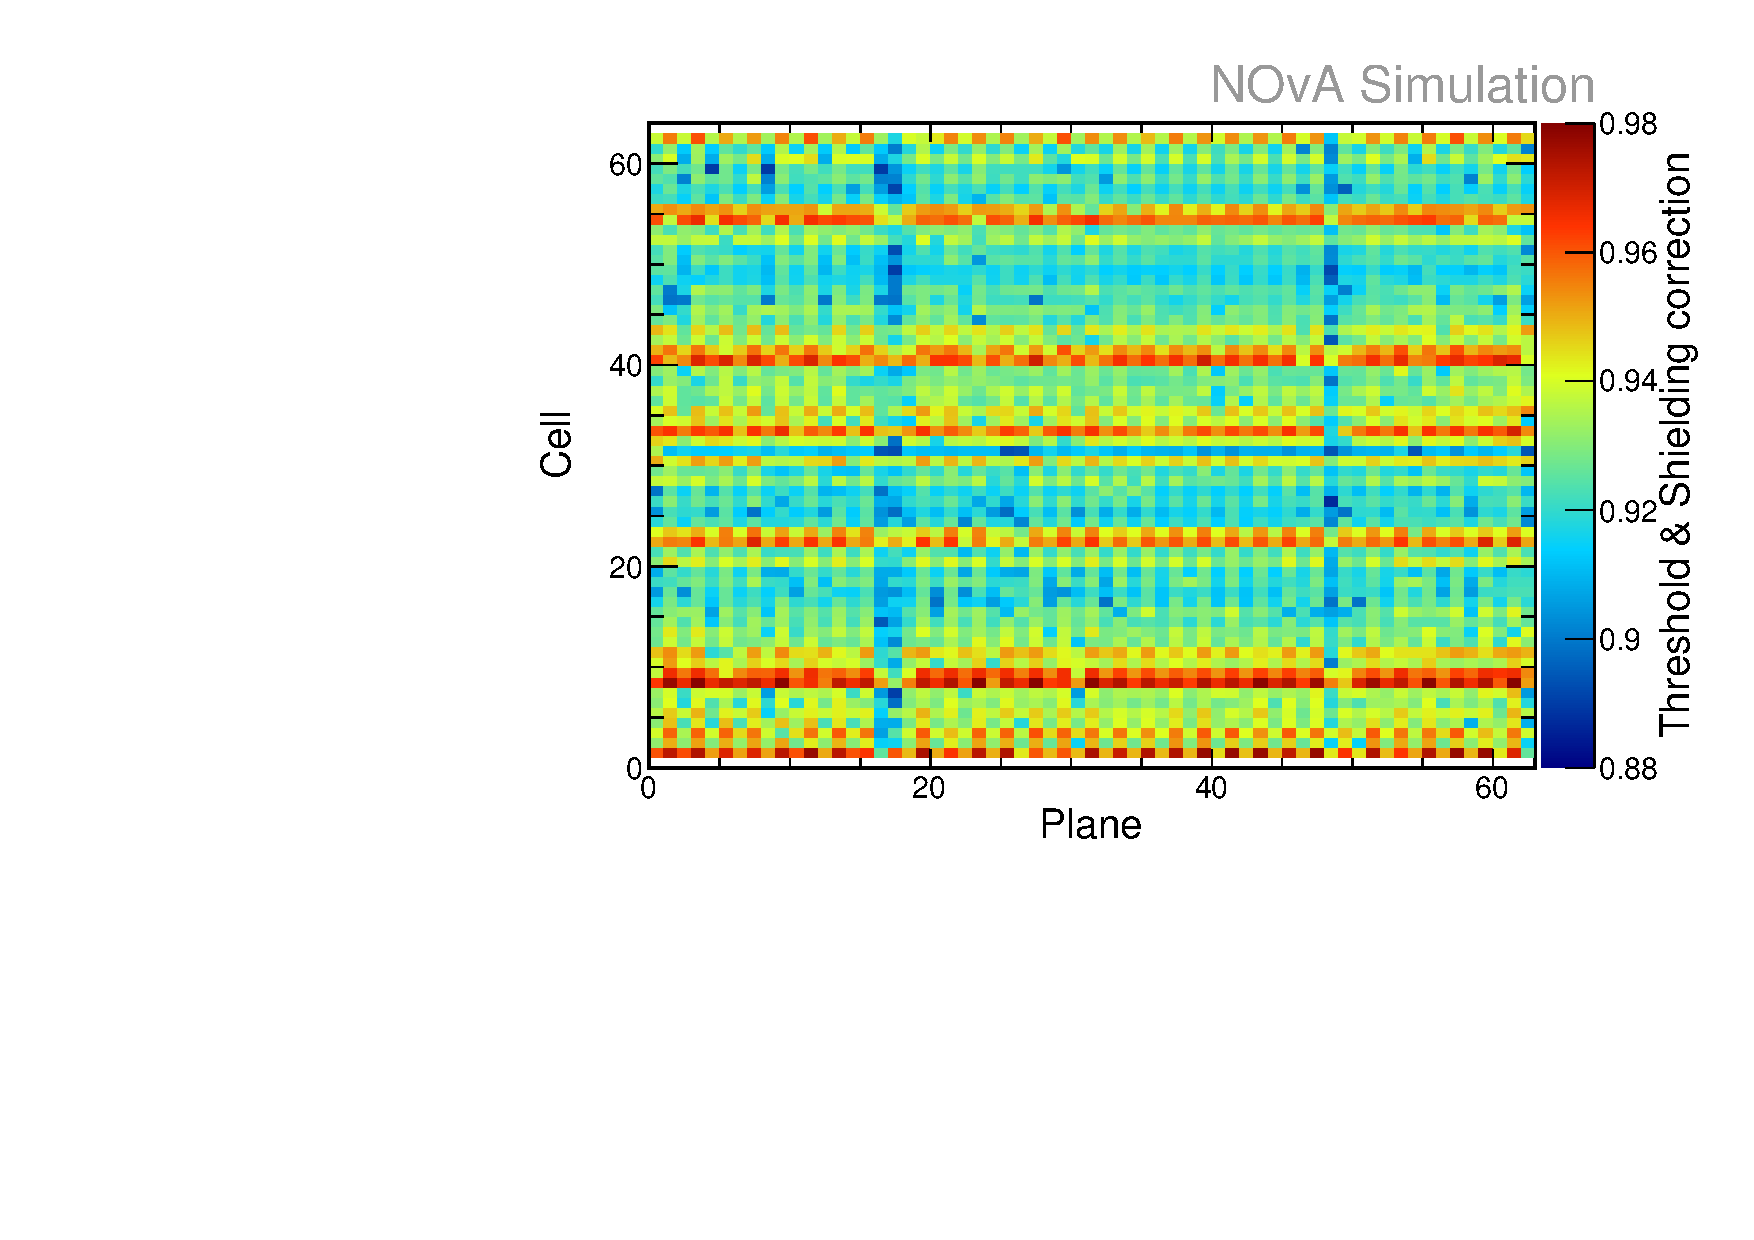
\includegraphics[width=.8\textwidth]{Plots/TBCalibration/ThresholdCorrectionMap_P4DataBasedSim.pdf}
\end{subfigure}
\begin{subfigure}[b]{\textwidth}
\centering
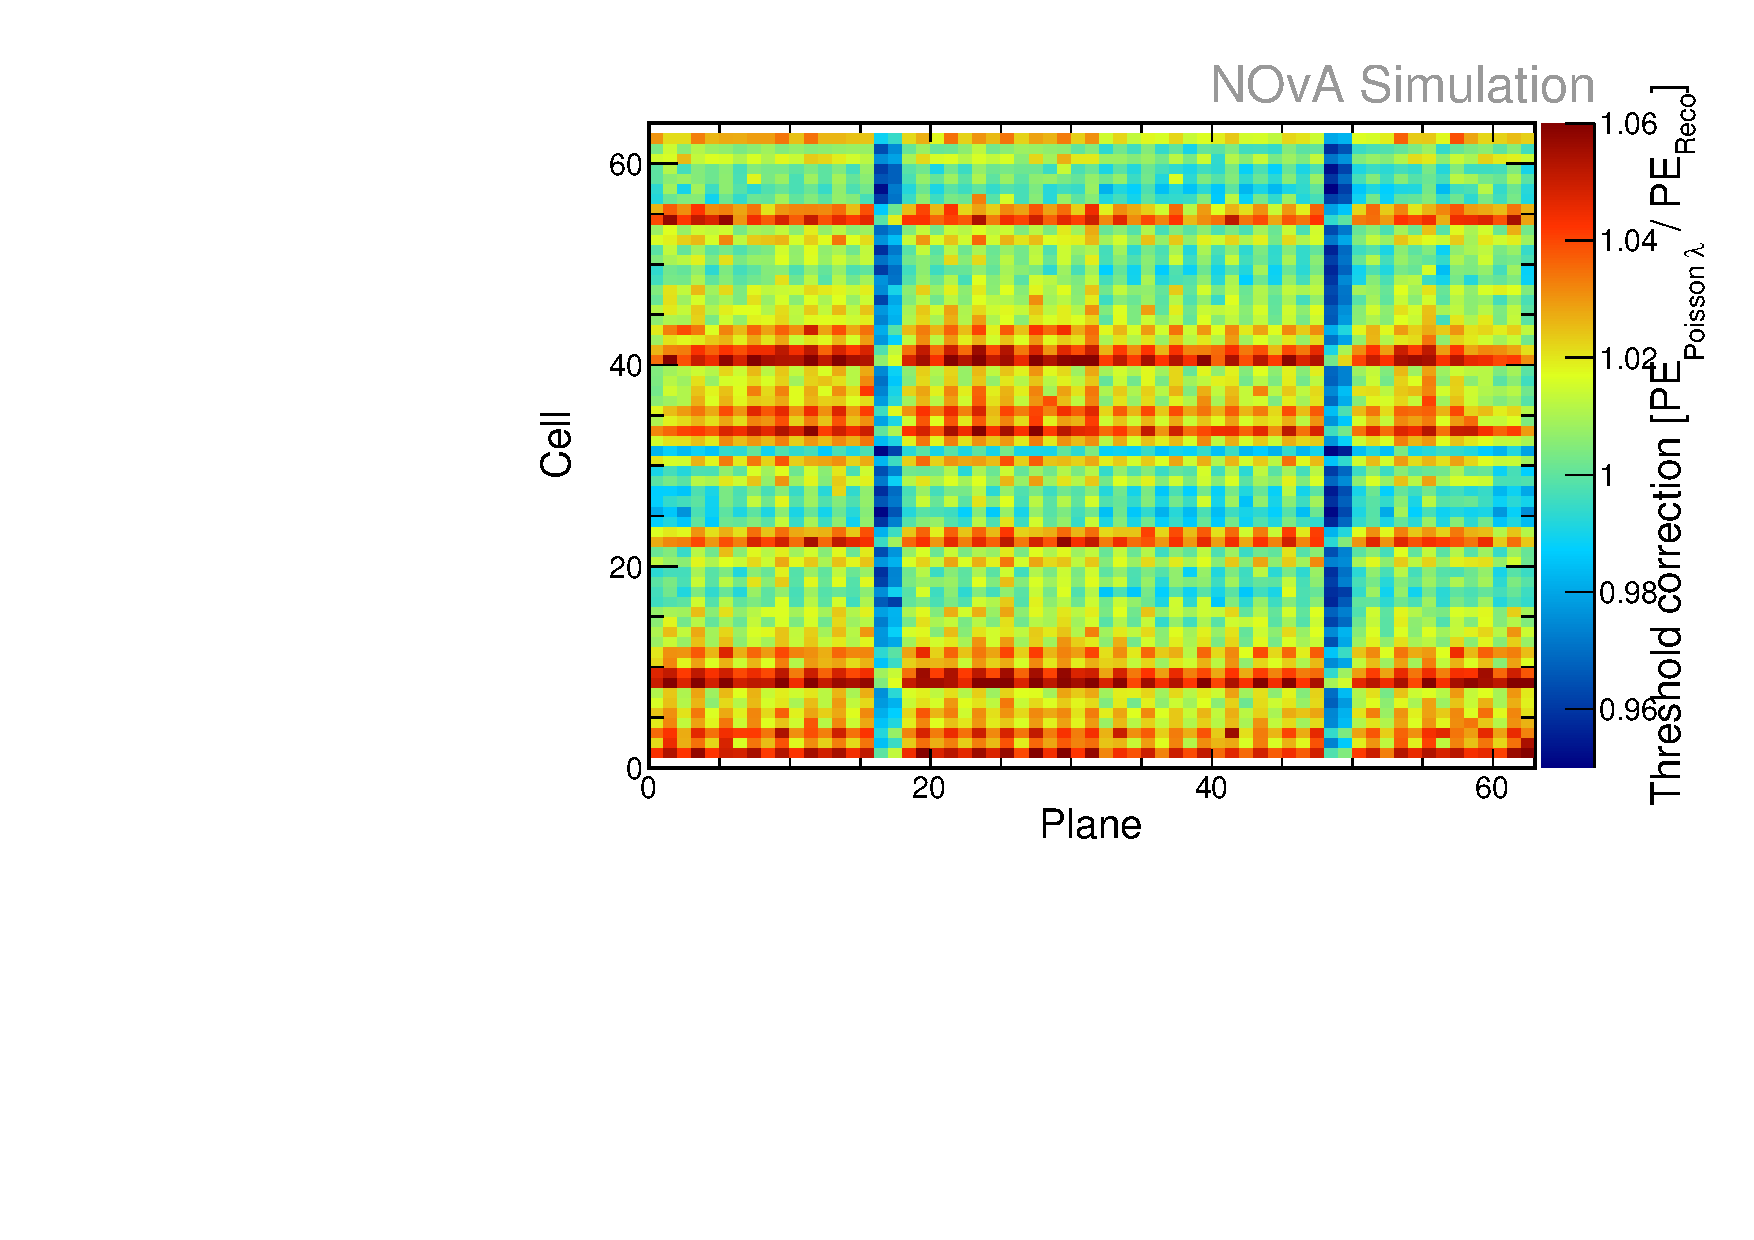
\includegraphics[width=.8\textwidth]{Plots/TBCalibration/ThresholdOnlyCorrectionMap_P4DataBasedSim.pdf}
\end{subfigure}
\caption[Map of the threshold and shielding correction across the Test Beam detector]{Map of the threshold and shielding correction (top) and only of the threshold part of the correction (bottom) as a function of the Test Beam detector's cell and plane number. Each bin shows the mean correction for all the simulated events in that cell.}
\label{fig:TBThresholdCorrectionMap}
\end{figure}

%What is the threshold correction
The threshold part of the correction can be expressed as
\begin{equation}
\textsf{Threshold correction}=\frac{\gls{PE}_{Poisson \lambda}}{\gls{PE}_{Reco}},
\end{equation}
where $\gls{PE}_{Poisson \lambda}$ represents the mean of the Poisson distribution of the true deposited energy (in terms of $\gls{PE}_{True}$), and $\gls{PE}_{Reco}$ is the reconstructed number of \gls{PE} from simulation. Both $\gls{PE}_{Poisson \lambda}$ and $\gls{PE}_{True}$ are direct outputs of the light model simulation, as detailed in Sec.~\ref{sec:NOvASimulation}. After the light model simulation, $\gls{PE}_{True}$ is passed through the readout simulation, which includes a \gls{PE}-to-\gls{ADC} function for calculating the peak \gls{ADC} value. This value is then converted into $\gls{PE}_{Reco}$ using the \gls{ADC}-to-\gls{PE} scale described in Sec.~\ref{sec:NOvACalibration}. The observed shape in the threshold correction can thus be attributed to differences between $\gls{PE}_{True}$ and $\gls{PE}_{Poisson \lambda}$, as well as to various effects introduced by the readout simulation. However, the differences between $\gls{PE}_{True}$ and $\gls{PE}_{Poisson \lambda}$ are marginal (below $\unit[1]{\%}$) and contribute minimally to the threshold correction. Therefore, the predominant influence on the observed pattern comes from the effects introduced by the readout simulation.

%FEB versions
There are two prominent features in the threshold correction variations in Fig.~\ref{fig:TBThresholdCorrectionMap}. Firstly, the two blue vertical lines in planes 16-17 and 48-49. These planes are using the \gls{FEB} version 5.2, used in the \gls{ND}, instead of  the \gls{FEB} version 4.1, used in the \gls{FD} and in all the other Test Beam planes, as explained in Sec.~\ref{sec:TBExperiment}. Both the readout simulation and the \gls{ADC}-to-\gls{PE} scale do account for the expected disparity in the \gls{ADC}/\gls{PE} ratio between the two \gls{FEB} versions. However, it is expected that \gls{FEB}v5 would exhibit a lower response to the same energy compared to \gls{FEB}v4. Therefore, for the same $\gls{PE}_{Poisson \lambda}$ values, the $\gls{PE}_{Reco}$ for \gls{FEB}v5 should be smaller than that for \gls{FEB}v4. Consequently, the \gls{FEB}v5 planes should have a larger threshold correction compared to the \gls{FEB}v4. However, as was shown in Fig.~\ref{fig:TBThresholdCorrectionMap}, the observed correction is contrary to this expectation, suggesting a potential error in the readout simulation regarding the handling of different \gls{FEB} versions.

%APD relative gain map
The second notable feature in Fig.~\ref{fig:TBThresholdCorrectionMap} is the variation of the threshold correction across cells, which appears to be consistent across all planes, depicted by the presence of red horizontal lines. The origin of this dependency is in the \gls{APD} structure, where each \gls{APD} collects signal from 32 cells arranged in 4 rows of 8 \gls{APD} pixels, as explained in Sec.~\ref{sec:DAQ}. Manufacturing discrepancies \cite{NOvA-doc-5239} lead to relative gain variations among the \gls{APD} pixels, typically exhibiting either increasing or decreasing trend along each of the four rows. To incorporate these variations into the readout simulation, the mean relative gain across cells of every module (comprising 32 cells) is used in the \gls{PE}-to-\gls{ADC} function. Consequently, these variations are consistent across all modules in the simulated detector, despite their inherent randomness in actual data.

The distribution of the relative gain for each `pixel number' is shown on the left of Fig.~\ref{fig:TBThresholdCorrectionGainMap}. However, it is important to note that `pixel number' is a \gls{NOvA} jargon and does not correspond directly to the \gls{APD} pixel position or cell number; instead it denotes the purely technical routing of \gls{APD} pixels to the \gls{FEB} \cite{NOvA-doc-11570}. Therefore, the depicted distribution of gain variation on the left of Fig.~\ref{fig:TBThresholdCorrectionGainMap} is incorrect and should instead describe the distribution with respect to the cell number rather than the `pixel number'. Simply translating `pixel numbers' to cell numbers yields the distribution shown on the right of Fig.~\ref{fig:TBThresholdCorrectionGainMap}. Comparing this to the positions of the red horizontal lines in Fig.~\ref{fig:TBThresholdCorrectionMap} demonstrates that this (incorrect) relative gain variation is responsible for the observed pattern in the threshold correction.

\begin{figure}[!hbtp]
\centering
\begin{subfigure}[t]{.495\textwidth}
\centering
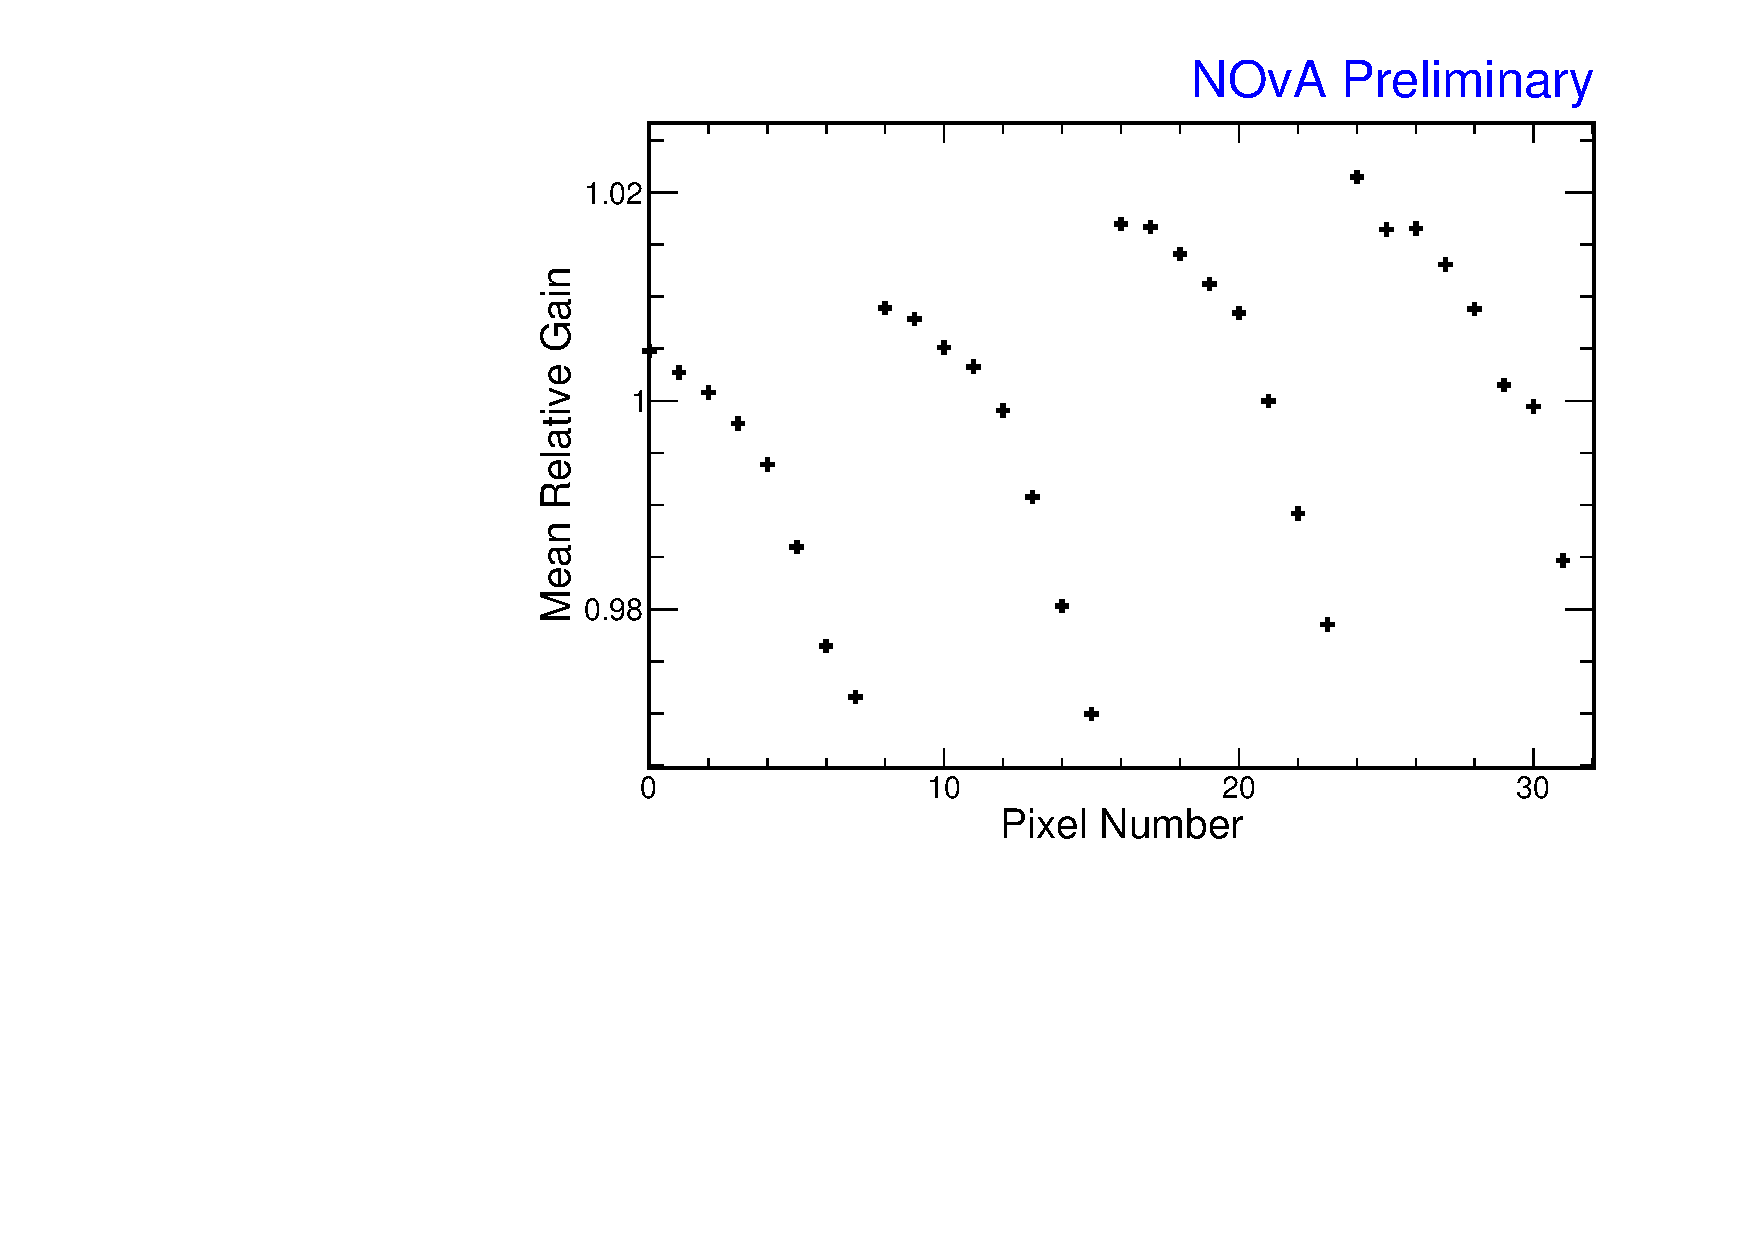
\includegraphics[width=\textwidth]{Plots/TBCalibration/ReadoutSimulation_GainPixelMap.pdf}
\end{subfigure}
\begin{subfigure}[t]{.495\textwidth}
\centering
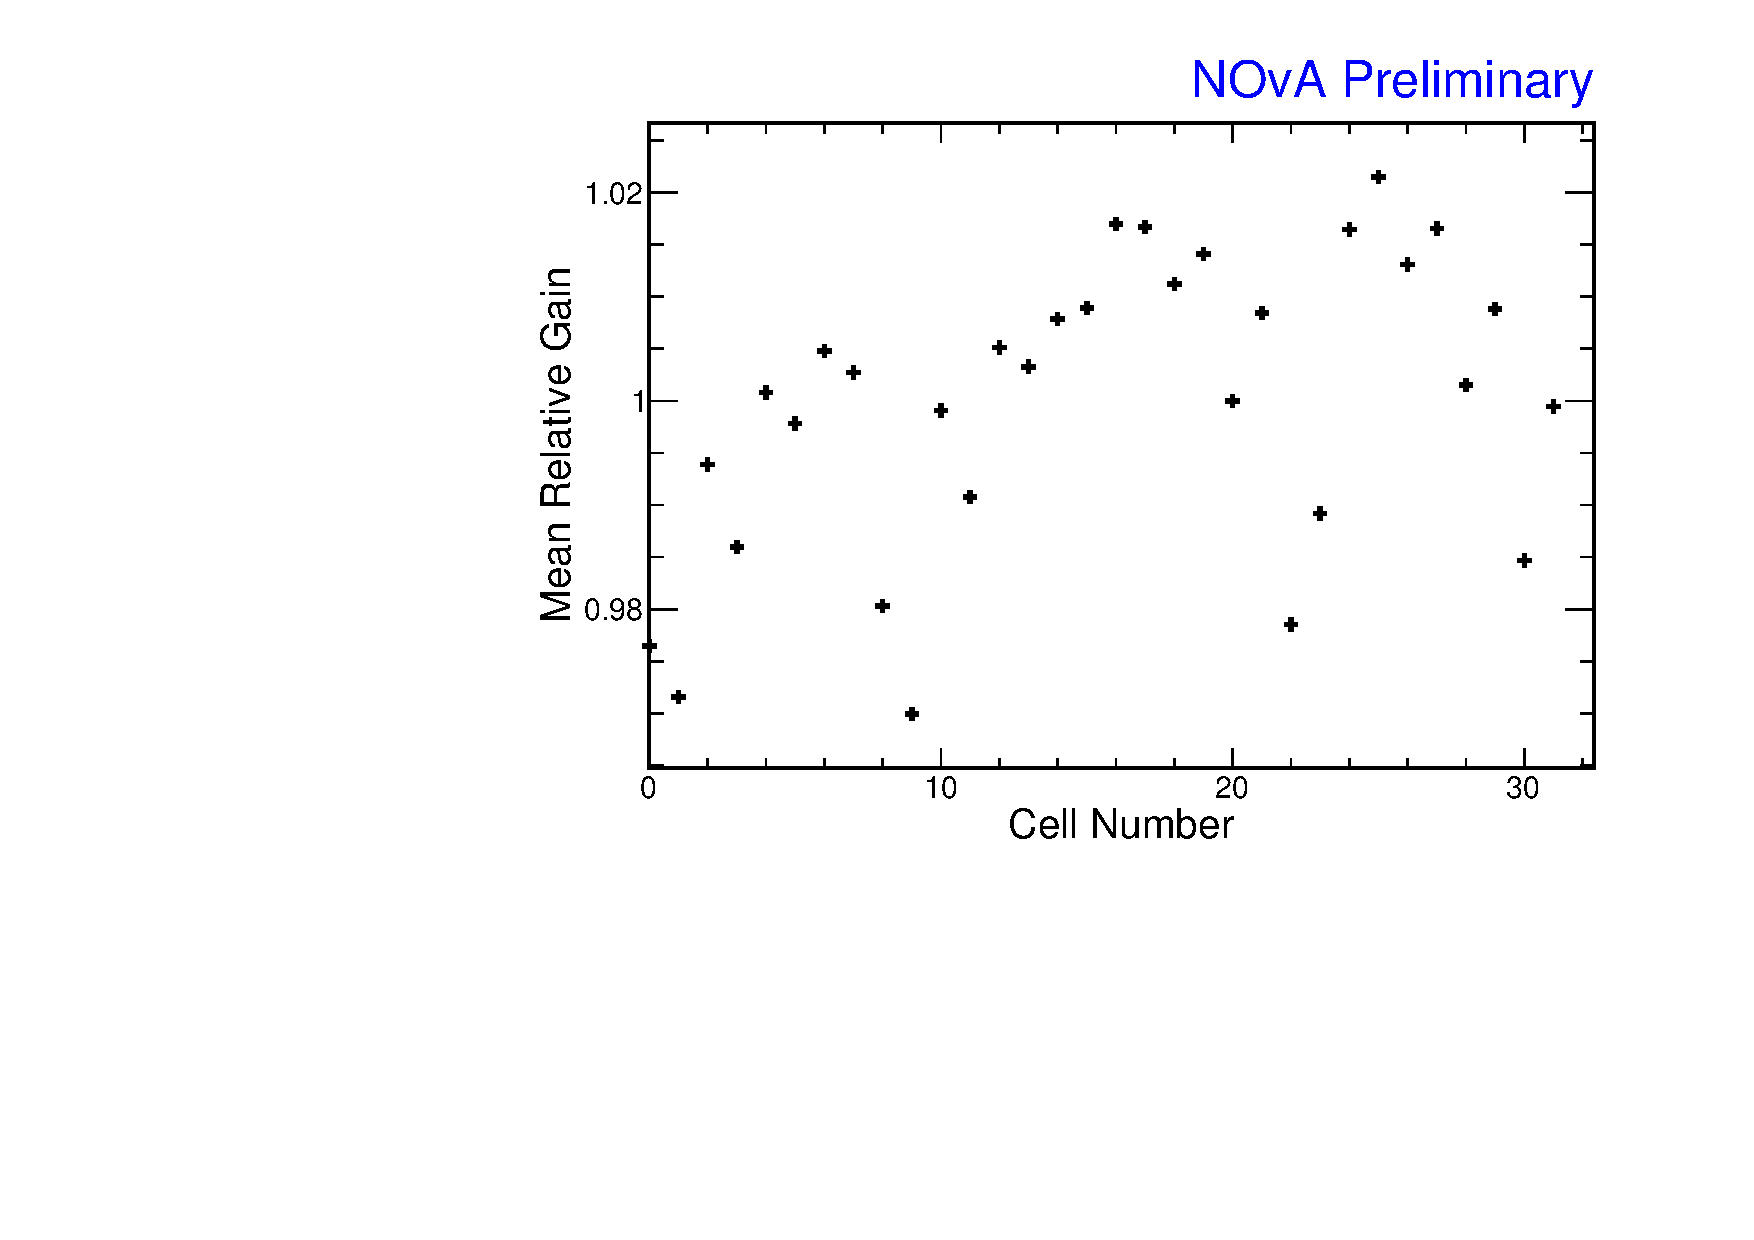
\includegraphics[width=\textwidth]{Plots/TBCalibration/ReadoutSimulation_GainCellMap.pdf}
\end{subfigure}
\caption{The relative gain variation as a function of the `pixel number' (left) and cell number (right).}
\label{fig:TBThresholdCorrectionGainMap}
\end{figure}

%Conclusion
In summary, the threshold and shielding correction exhibits significant variations concentrated within specific planes and cells, arising from various effects in the readout simulation. However, it is evident that these effects are not limited to cosmic events and therefore should not be incorporated into the threshold and shielding correction. Given that these effects are corrected out for simulation before the attenuation fits, they are not accounted for in the relative calibration and therefore remain present for the absolute calibration and for beam events. Moreover, the two main effects outline above are not implemented into the simulation correctly, resulting in discrepancies between actual data and simulation. This means, that in data these variations are either not present or present in a different way than in simulation. Therefore, applying the simulation-based threshold and shielding corrections to data introduces new variations that would otherwise not exist for data. As a result, these new variations are incorporated into the attenuation fits for data, resulting in incorrect relative calibration results applied to both absolute calibration and beam events.

%future, solutions
Several approaches can address these issues. For simulation-related discrepancies, the only viable solution is to rectify the identified faults and to remake the simulation, albeit this would be computationally very intensive. However, for data-related concerns, efforts are underway to devise a new data-driven threshold and shielding correction \cite{NOvA-doc-15223}, eliminating any influence of simulation on the relative calibration of data. If a purely data-driven correction is not viable, there is another possible improvement to the threshold correction while still using simulation, which is to not use the $\gls{PE}_{Poisson \lambda}$ directly, but to pass it through the readout simulation in the same way as $\gls{PE}_{True}$ and create an alternative $\gls{PE}_{Poisson \lambda Reco}$.

\subsection{Simulation}\label{sec:SimulationResults}
The distribution of tricell hits from the simulated cosmic muon events selected for calibration, mapped across the Test Beam detector's planes and cells, is shown in Fig.~\ref{fig:CalibhistSim}. As this is a simulated detector, we will use this `ideal conditions' distribution of tricell hits to illustrate the main features, which are also present in all the data samples discussed below. We can clearly see the difference in the number of events between the vertical (even) and the horizontal (odd) planes. This is expected as cosmic muons are generally vertical and a single cosmic track often passes more horizontal planes than vertical planes. We can also see that due to the tricell condition there are no hits in cells 0 and 63, which are on the edge of the detector. These cells can still be calibrated by including hits from the `z tricell' condition, which is not shown in the plot. The three clear horizontal lines of relatively lower response going across the detector correspond to pairs of cells 15 + 16, 31 + 32, and 47 + 48. Together with cells 0 and 63, they represent the first and the last cells of each 16 cell-wide extrusion, which makes up half of a module, which in turn makes up half of a Test Beam plane. As was mentioned in Sec.~\ref{sec:NOvADetectors}, these cells are $\unit[3]{mm}$ narrower than the rest, resulting in fewer hits and a lower deposited energy. However, using the deposited energy divided by path length for calibration should compensate for this effect. Overall, Fig.~\ref{fig:CalibhistSim} demonstrates that the tricell hits are distributed fairly uniformly in the centre of the detector, with the number of hits dropping off towards the front, back and corners of the detector. This is a result of the event selection applied to the cosmic tracks for calibration.

\begin{figure}[h]
\centering
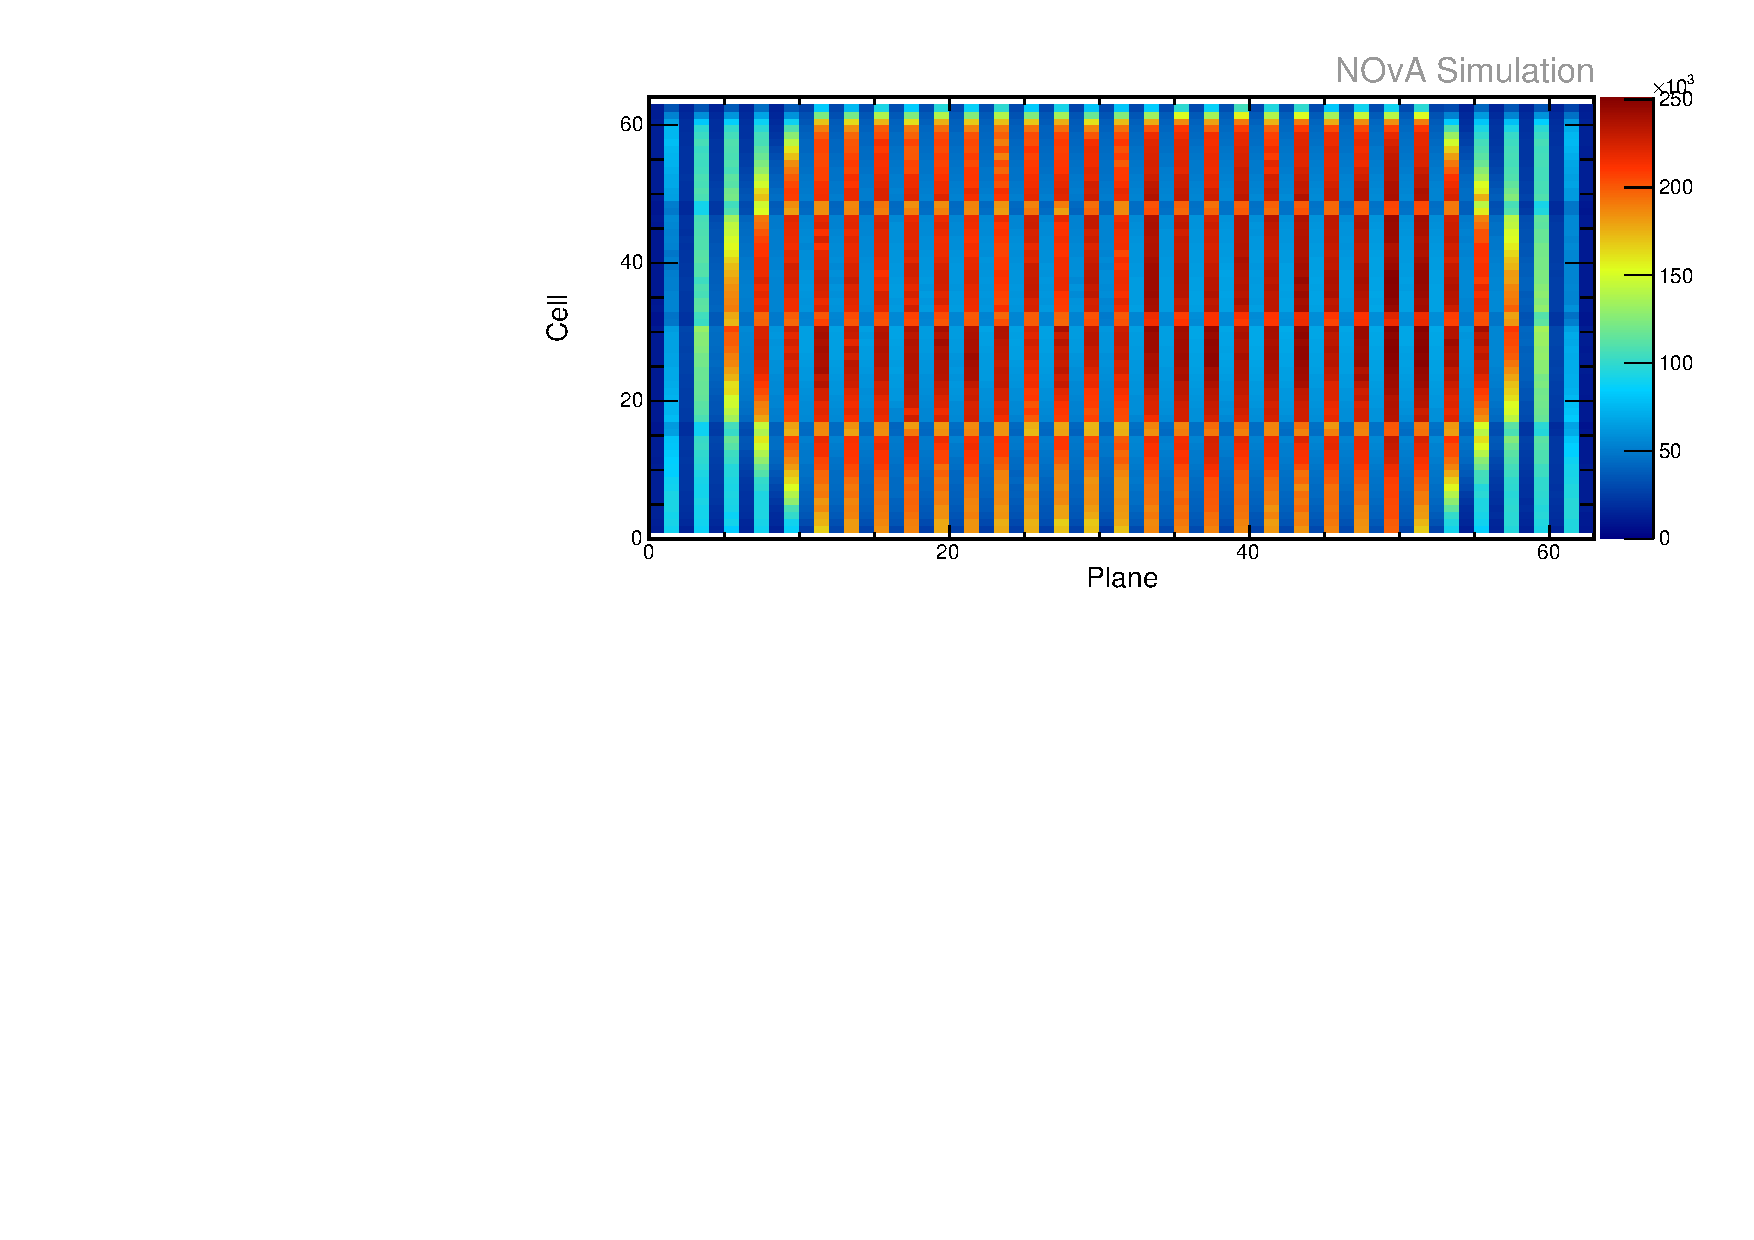
\includegraphics[width=\textwidth]{Plots/TBCalibration/Attenprofs_Simulation_CellPlane.pdf}
\caption[Plane-Cell distribution of hits for the simulation sample]{Distribution of tricell hits used for the calibration of the simulated Test Beam detector. Features are described in text.}
\label{fig:CalibhistSim}
\end{figure}

The distributions of deposited energy per path length though the cell before the calibration in units of $\unit{PE/cm}$ as a function of $w$, cell and plane number, are shown in Fig.~\ref{fig:Calibhist_simulation}. These distributions should be uniform after applying the results of the calibration and can be used to identify the main features that will need to be corrected for during the calibration. The shallow rise of the energy response along $w$ is caused by the attenuation of light along the \gls{WLS} fibres. The drop in the response at the edges of the cell is caused by the fibres looping and connecting to the \glspl{APD}, while the larger statistical uncertainties at the edges of the cell reflect the lower number of hits passing the event selection including the tricell condition.

\begin{figure}[h]
\centering
\begin{subfigure}[b]{0.495\textwidth}
\centering
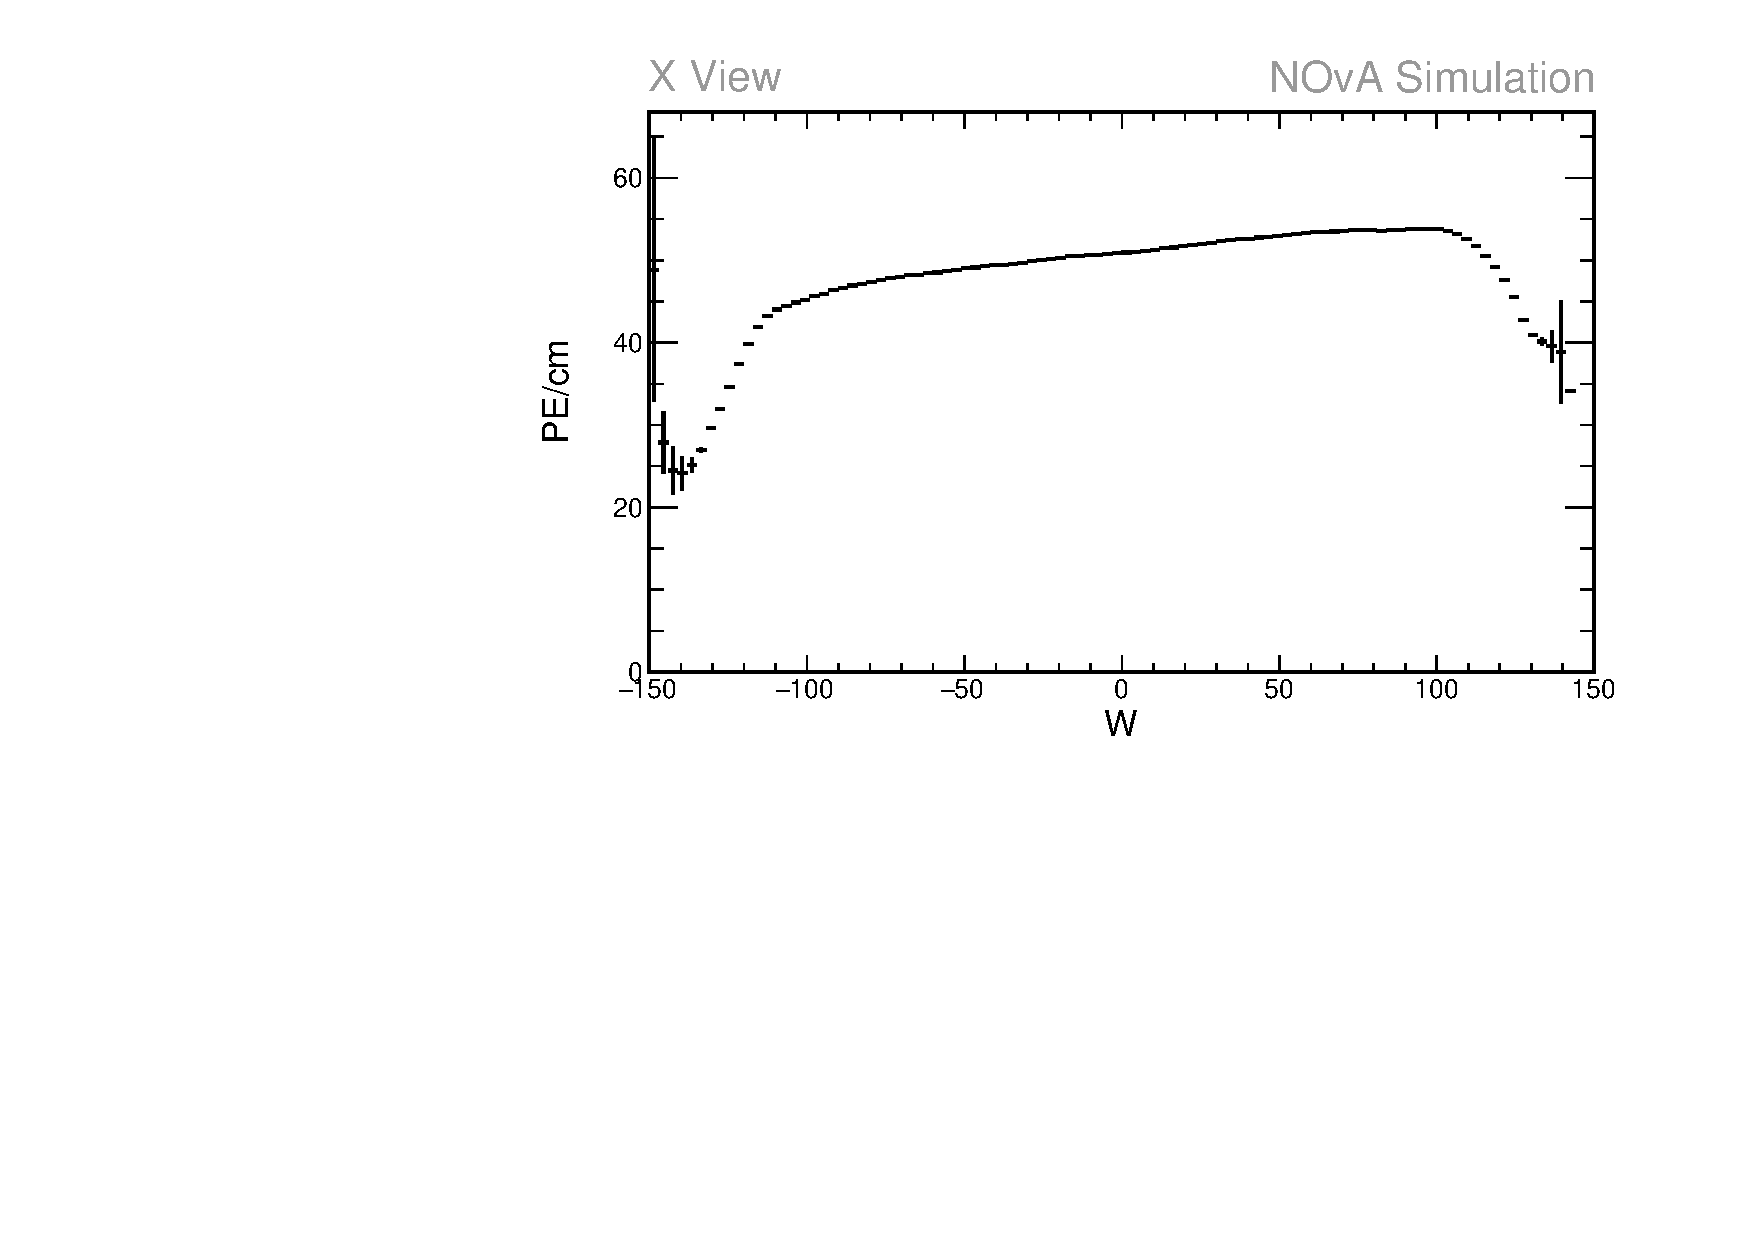
\includegraphics[width=\textwidth]{Plots/TBCalibration/Attenprofs_Simulation_WPE_corr_xy_X_Prof.pdf}
\end{subfigure}
\begin{subfigure}[b]{0.495\textwidth}
\centering
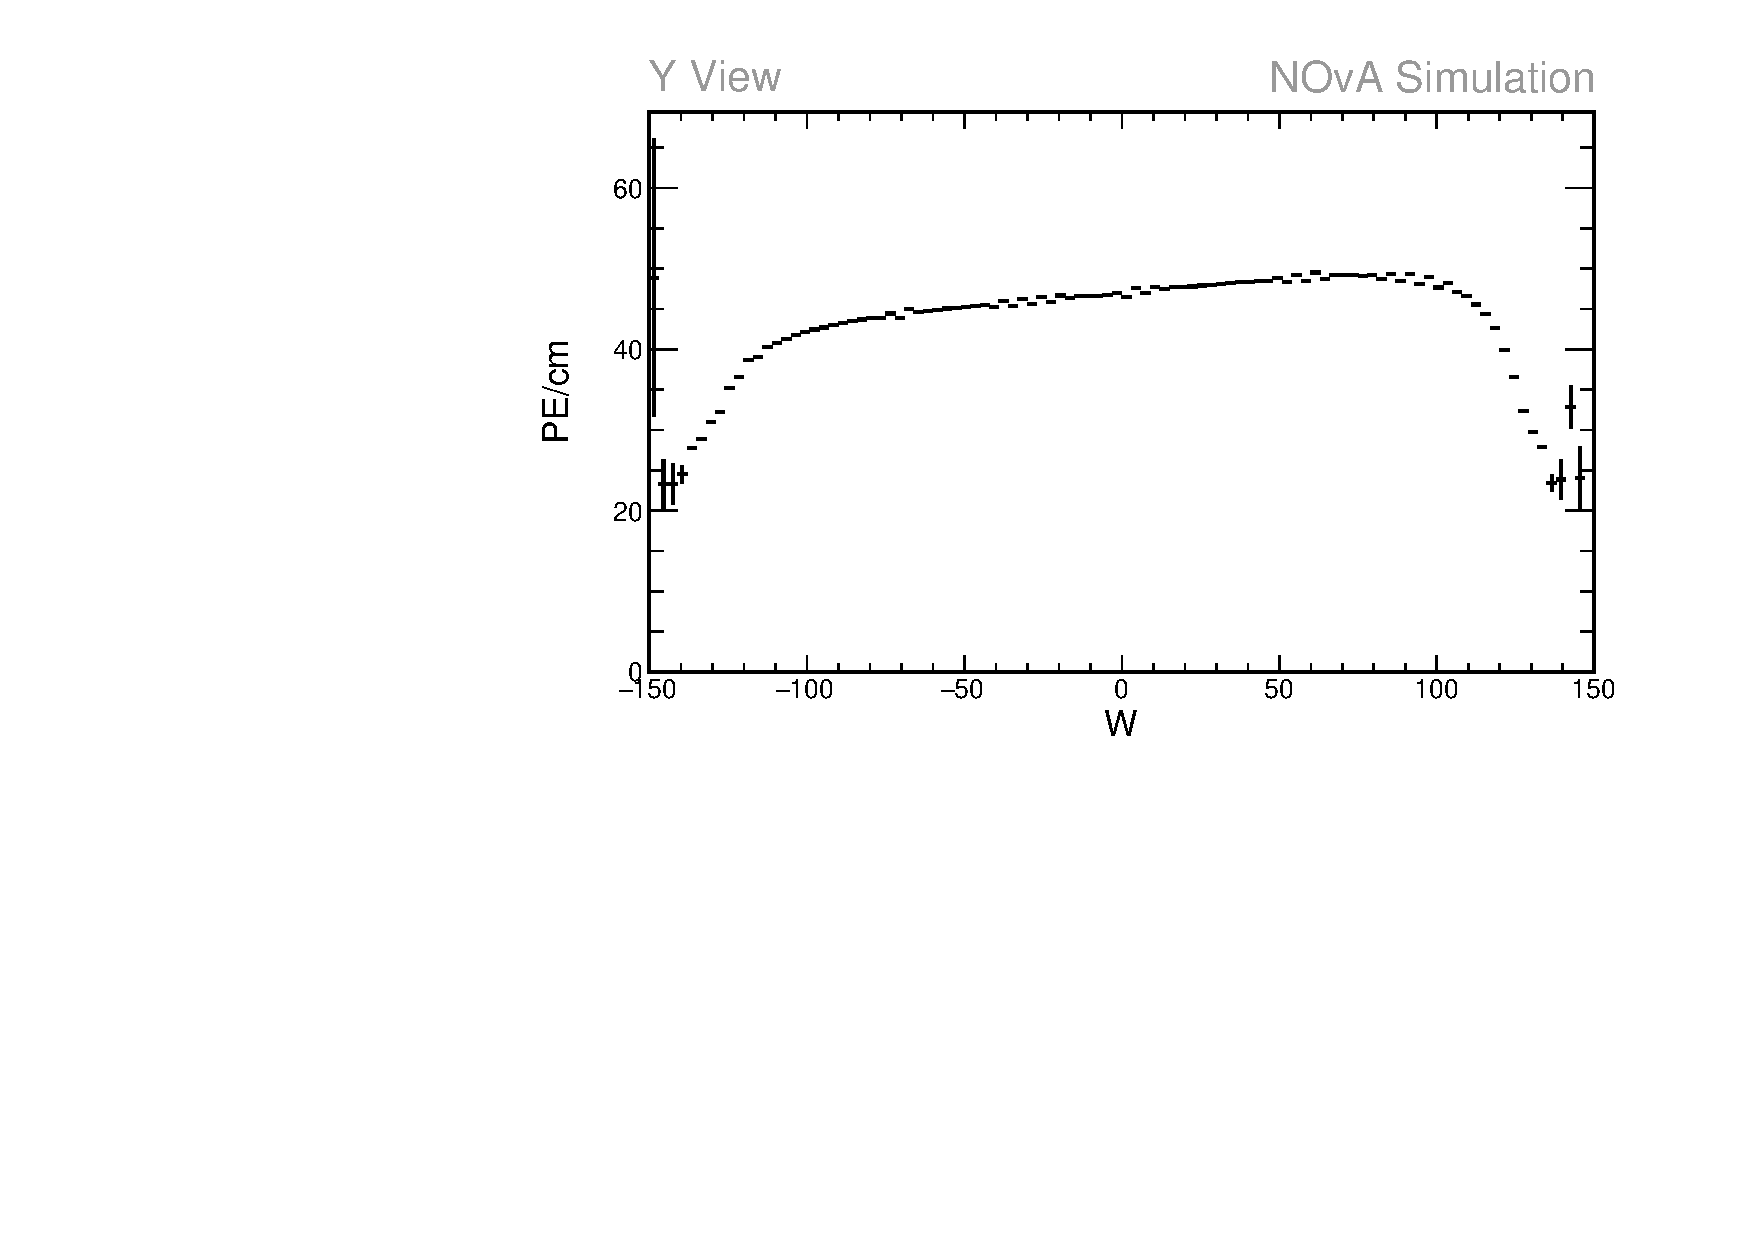
\includegraphics[width=\textwidth]{Plots/TBCalibration/Attenprofs_Simulation_WPE_corr_xy_Y_Prof.pdf}
\end{subfigure}
\begin{subfigure}[b]{0.495\textwidth}
\centering
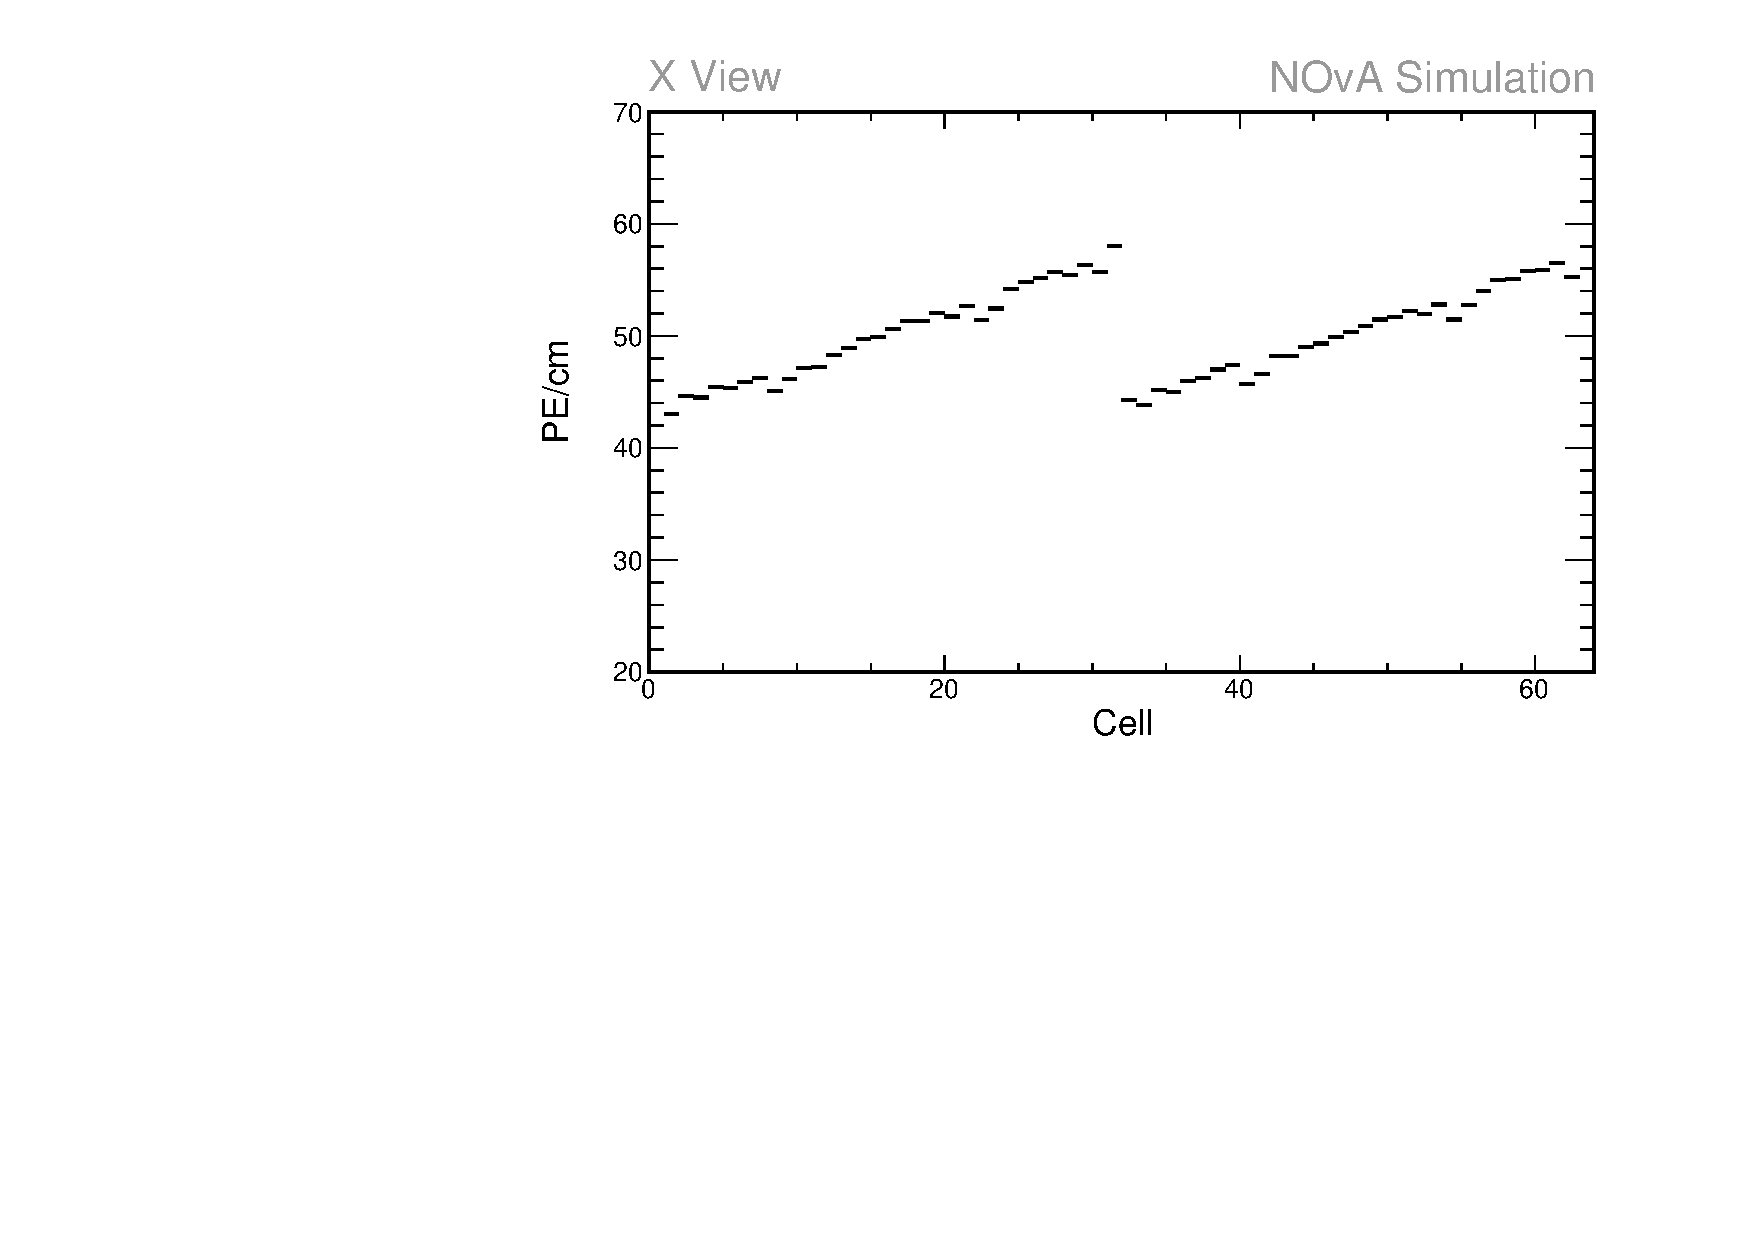
\includegraphics[width=\textwidth]{Plots/TBCalibration/Attenprofs_Simulation_CellPE_X_Prof.pdf}
\end{subfigure}
\begin{subfigure}[b]{0.495\textwidth}
\centering
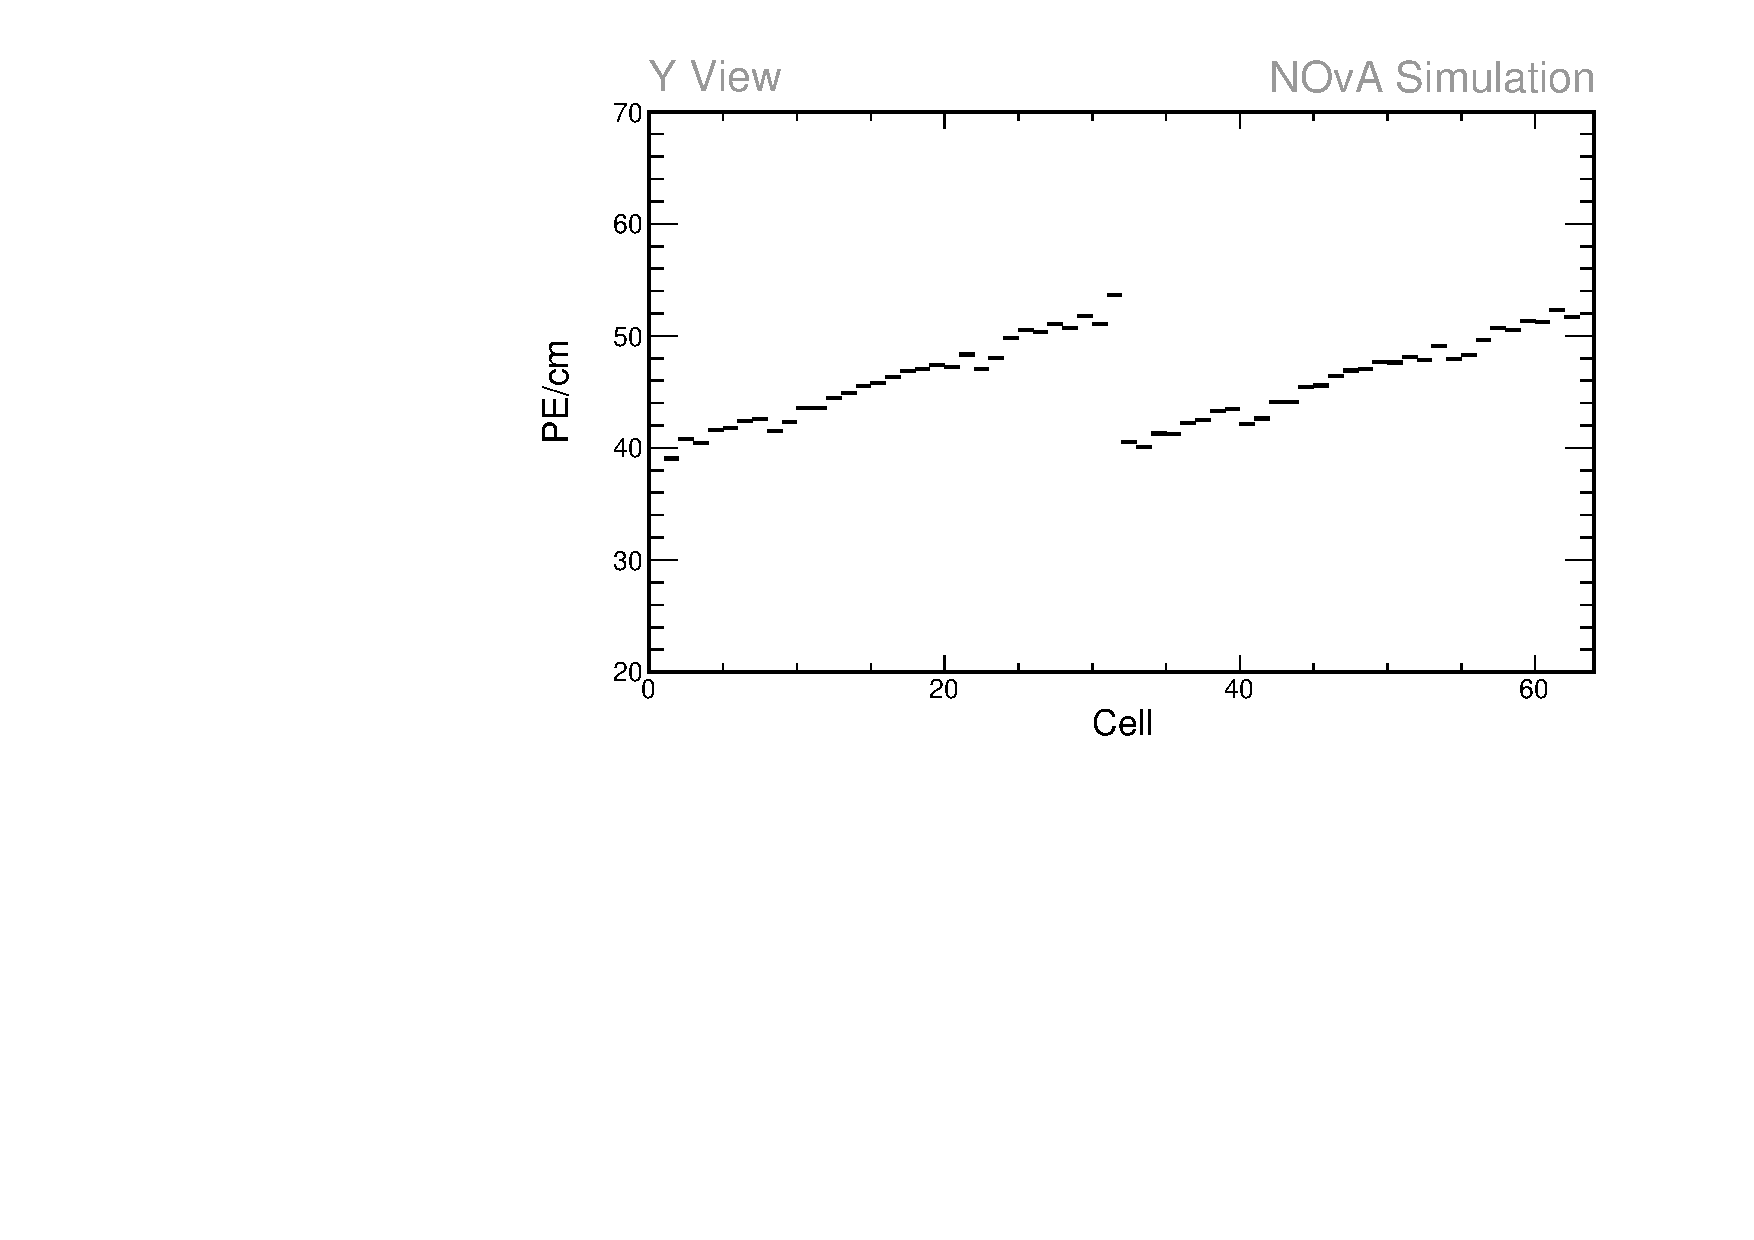
\includegraphics[width=\textwidth]{Plots/TBCalibration/Attenprofs_Simulation_CellPE_Y_Prof.pdf}
\end{subfigure}
\begin{subfigure}[b]{0.495\textwidth}
\centering
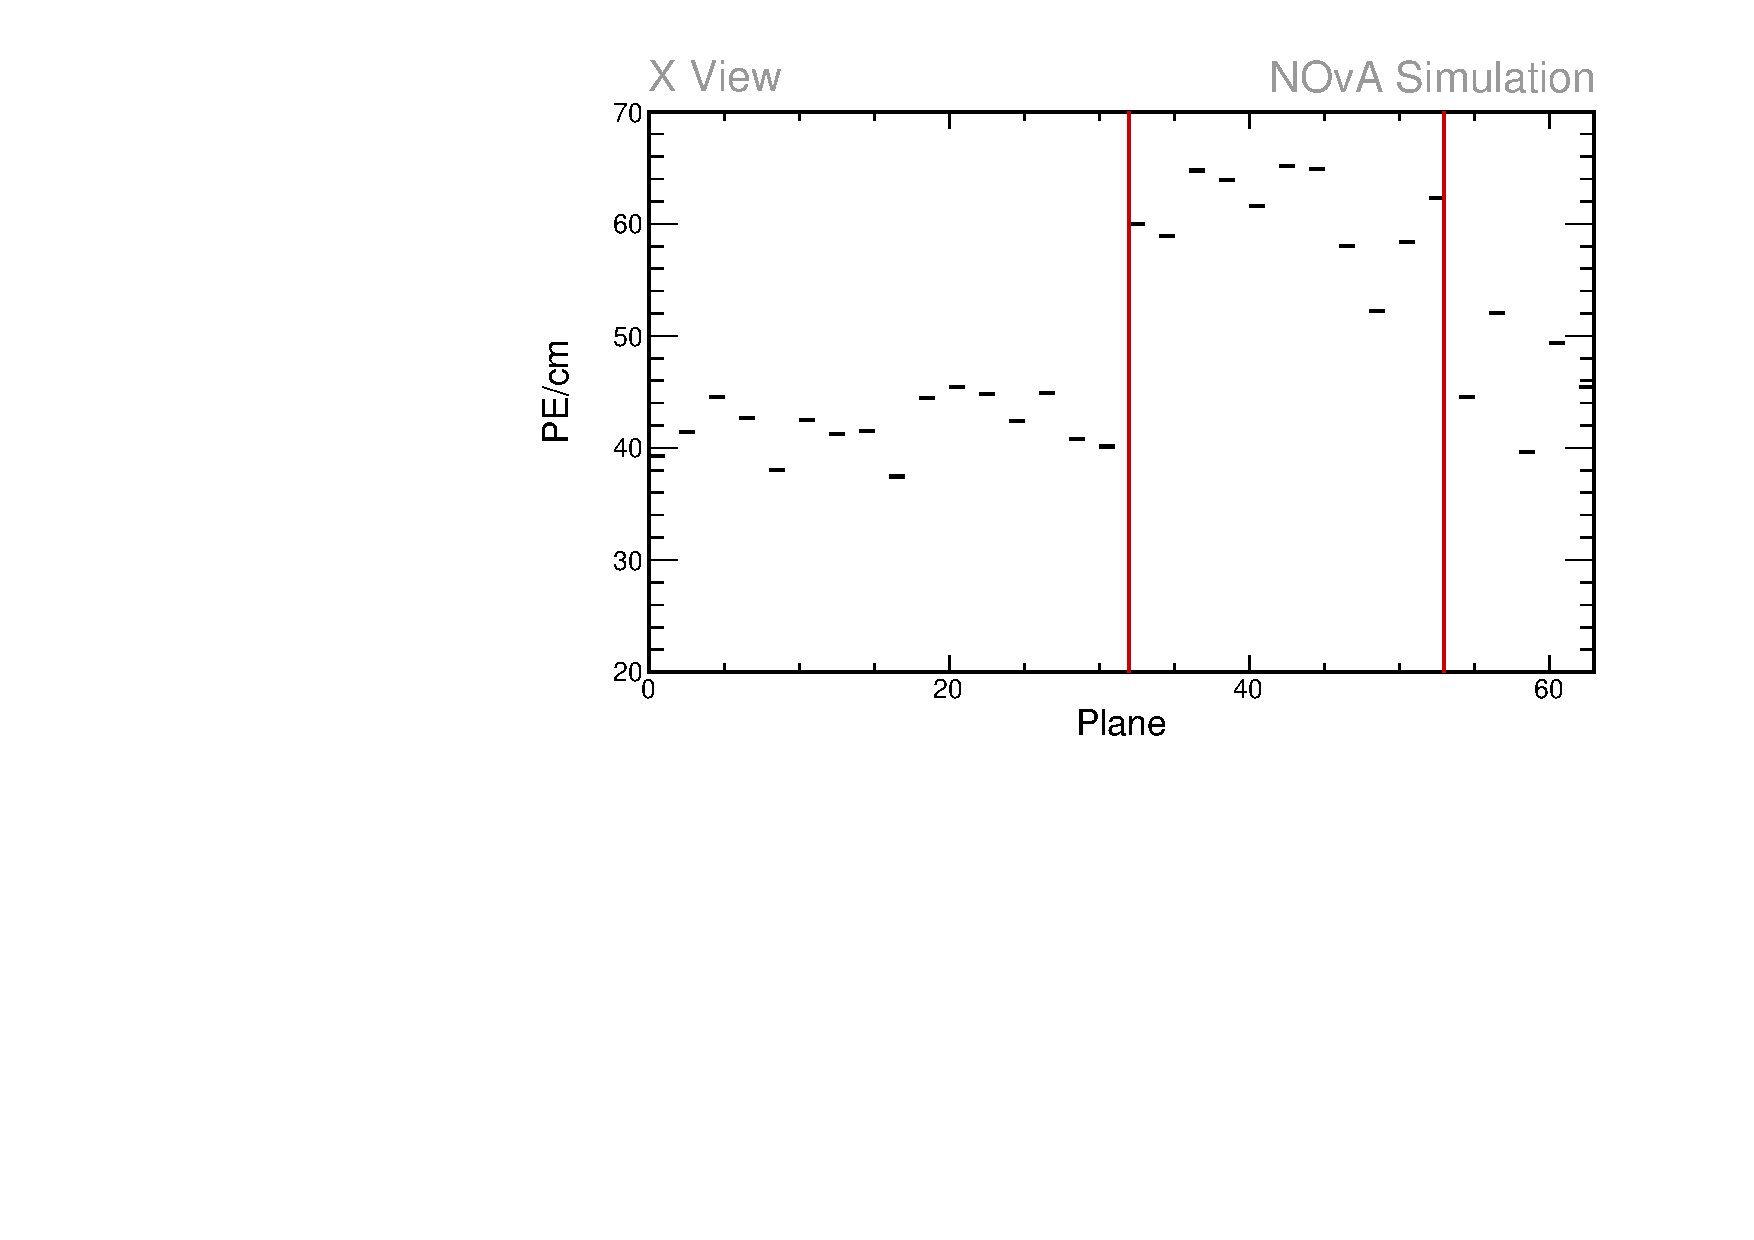
\includegraphics[width=\textwidth]{Plots/TBCalibration/Attenprofs_Simulation_PlanePE_X_Prof.pdf}
\end{subfigure}
\begin{subfigure}[b]{0.495\textwidth}
\centering
\includegraphics[width=\textwidth]{Plots/TBCalibration/Attenprofs_Simulation_PlanePE_Y_Prof.pdf}
\end{subfigure}
\caption[Uncorrected energy response along $w$, cell and plane for simulation]{Uncorrected average energy response as a function of the position within a cell ($w$ - top), cell number (middle), or plane number (bottom) for the Test Beam detector simulation of cosmic muon hits selected for calibration. Left side shows distributions for the X view (vertical) planes and right side for the Y view (horizontal) planes. Each plot is a profile histogram, with uncertainties representing statistical variations. Red lines on the bottom two plots depict the boundaries between different scintillators. Features explained in text.}
\label{fig:Calibhist_simulation}
\end{figure}

The rise of the response with the cell number, visible in the middle plots in Fig.~\ref{fig:Calibhist_simulation}, is due to the varying distance of cells to the readout. Since the \glspl{APD} are located on one side of each module, light from cells on the opposite side has to travel along the \gls{WLS} fibre for an additional module width, compared to the cells closer to the readout. Light undergoes additional attenuation along these so-called `pig tails', causing the difference of the energy response. The additional variations across cells within a module, notably the relatively lower response in cells 0, 1, 9, 10, 23, 24, 31 and 32, is caused by including the relative gain differences into the simulation, as explained above in Sec.~\ref{sec:TBThresholdCorrection}.

The uncorrected energy response as a function of plane number is shown in the bottom row of Fig.~\ref{fig:Calibhist_simulation}, illustrating large fluctuations between planes in both views. We can clearly identify the three distinctly different responses delineated by red lines, corresponding to the three scintillator variations used, as described in Sec.\ref{sec:TBExperiment}. Additionally, planes 16, 17, 48 and 49 use the \gls{FEB}v5.2 instead of \gls{FEB}v4.1, resulting in a relatively lower response. All these variations between planes originate from the \gls{FB} map (Sec.~\ref{sec:FibreBrightnessTB}),  which is used for simulation to emulate real detector conditions. The rest of the variations are caused by differences between readout electronics and individual cells, but are exacerbated by the \gls{FB} binning, which groups otherwise smooth variations across planes into 12 discrete bins, thus amplifying them. \note{Not sure if the last point is clear and if it makes sense}

\subsubsection*{Simulation Relative Calibration Results}

An overview of the attenuation fit results for simulation is shown in Fig.~\ref{fig:CellCentreResponseSim} as a map of average fitted response in the centre of each cell. Blank cells mark the uncalibrated cells which failed the calibration condition (attenuation fit $\chi^2>0.2$). All the uncalibrated cells but one are on the edges of the detector, which is expected, as they have much fewer events that pass the calibration sample selection. There are 43 uncalibrated cells out of the total 4032 cells in the Test Beam detector, resulting in 1.07\% of the simulated detector remaining uncalibrated.

\begin{figure}[h]
\centering
\includegraphics[width=\textwidth]{Plots/TBCalibration/CellResponseAtCentre_Prod4DataBasedSim_Limited_NOvAPlotStyle.pdf}
\caption[Map of fitted response at cell centre for simulation]{Overview of the attenuation fit results for the simulated Test Beam detector. Each cell represents the result of the attenuation fit to the energy response in the centre of that cell. The blank cells are uncalibrated as the attenuation fit did not satisfy the calibration condition.}
\label{fig:CellCentreResponseSim}
\end{figure}

For simulation, the attenuation fit is done for each \gls{FB} bin and each cell separately. Examples of detector response for different cells in various \gls{FB} bins are shown in Fig.~\ref{fig:AttenfitResultsSimulation}. Here the red line shows the initial exponential fit and the blue line depicts the final attenuation fit after the \gls{LOWESS} correction, as described in Sec.~\ref{sec:NOvACalibration}. The cells on the edge of the detector failed the calibration conditions due to the low number of entries causing large fluctuation in the mean response.

There is only one cell in the middle of the detector that is left uncalibrated. This is the cell 32 in a vertical plane in \gls{FB} bin 5, shown on the top right of Fig.~\ref{fig:AttenfitResultsSimulation}, with $\chi^2=0.227$. Apparently, the reason the attenuation fit for this cell failed the calibration condition is the unusually high response with a large uncertainty in the right-most bin. It is unclear why this bin has such an elevated mean response, but since this only causes an issue for a single cell, we decided to ignore it and leave it uncalibrated \note{You are right that I should've marked this as calibrated manually as I'm doing with some other relative calibration results, but I didn't. Should I discuss it here, or rather in the discussion at the end of the chapter?}.

\begin{figure}[h]
  \begin{subfigure}{0.495\textwidth}
    \includegraphics[width=\linewidth]{Plots/RelativeCalibrationResults/sim_fb2_001_050.png}
  \end{subfigure}
  \begin{subfigure}{0.495\textwidth}
    \includegraphics[width=\linewidth]{Plots/RelativeCalibrationResults/sim_fb5_000_032.png}
  \end{subfigure}
  \begin{subfigure}{0.495\textwidth}
    \includegraphics[width=\linewidth]{Plots/RelativeCalibrationResults/sim_fb6_001_000.png}
  \end{subfigure}
  \begin{subfigure}{0.495\textwidth}
    \includegraphics[width=\linewidth]{Plots/RelativeCalibrationResults/sim_fb10_000_063.png}
  \end{subfigure}
  \caption[Example attenuation fits for simulation]{Attenuation fits for a selection of cells in various \acrshort{FB} bins in the calibration of the Test Beam simulation. Top left is an example of a successful attenuation fit, top right is a failed fit due to statistical fluctuation in the last bin and the bottom plots show failed fits for cells on the edges of the detector.}
  \label{fig:AttenfitResultsSimulation}
\end{figure}

\subsection{Period 2 Data}
The distribution of cosmic muon tricell hits selected for calibration in Test Beam period 2 data is shown in Fig.~\ref{fig:CalibhistMap_period2}.
The issue with underfilled cells described in Sec.~\ref{sec:TBExperiment} was present throughout period 2. The underfilled cells were marked as bad channels and therefore ignored during production of calibration samples. This also visibly affects the event count in the neighbouring cells to the underfilled cells, which have fewer calibration hits due to the tricell condition (see Sec.~\ref{sec:NOvACalibration}). However, since the underfilled cells 63 are also on the edge of the detector, labelling them as bad channels can't mitigate the effect on the neighbouring cells 62.

\begin{figure}[h]
\centering
\includegraphics[width=\textwidth]{Plots/TBCalibration/Attenprofs_P2Data_CellPlane_AllRuns.pdf}
\caption[Plane-Cell distribution of tricell hits for period 2 data]{Distribution of tricell hits as a function of Test Beam detector cells and planes in the entire period 2 data calibration sample. The rows of empty cells 31 and 62 across all the horizontal planes are caused by the underfilled cells (and tricell condition), as explained in text. There are several areas with relatively fewer hits. Notably cells 38-40 in plane 48 and cells 45-47 in plane 55. Both of these spots comprise of three cells, pointing towards the middle cell being a dead channel (for a limited time) and the two surrounding cells being affected by the tricell condition. Additionally, the bottom half of planes 55 and 57 have noticeably lower number of hits than their top halves (one half corresponds to a single readout).}
\label{fig:CalibhistMap_period2}
\end{figure}

We can also observe areas with relatively fewer hits, likely due to channels that were dead for some time. This also affects their immediate neighbours due to the tricell condition. Additionally, there are planes that have noticeably fewer hits in one half than in the other, and since half of a plane corresponds to a single readout (one \gls{FEB} and \gls{APD}), which means an entire readout was faulty for a certain time.

Officially, period 2 is divided into six epochs labelled 2a - 2f, based on specific Test Beam detector running conditions. Generally, smaller calibration samples reduce time-dependent effects on calibration, such as detector ageing or temperature and humidity variations. However, smaller samples also increase the number of cells with issues in the attenuation fit (examples shown below). Therefore, it is important to choose an optimal calibration sample size to balance both concerns. Since individual epochs in period 2 do not contain enough events for a successful attenuation fit, and variations between epochs are minimal, we decided to calibrate the entire period 2 together, without splitting it into any smaller calibration samples.

The epochs in period 2 mostly differ in the use of various \gls{FEB} firmwares or in the presence of trigger studies. We compare the energy deposition during the individual epochs in Fig.~\ref{fig:Calibhist_period2}. As can be seen, the difference between the energy response across the individual epochs is fairly small (within $\unit[2]{\%}$) and only in normalization, with the largest outliers seemingly epochs 2a and 2d. There is also no clear trend of energy response falling or raising with time (epoch labels are organized in time alphabetically).

\begin{figure}[!hbtp]
\centering
\begin{subfigure}[b]{0.495\textwidth}
\centering
\includegraphics[width=\textwidth]{Plots/TBCalibration/Attenprofs_P2Data_WPE_corr_xy_X_Combined.pdf}
\end{subfigure}
\begin{subfigure}[b]{0.495\textwidth}
\centering
\includegraphics[width=\textwidth]{Plots/TBCalibration/Attenprofs_P2Data_WPE_corr_xy_Y_Combined.pdf}
\end{subfigure}
\begin{subfigure}[b]{0.495\textwidth}
\centering
\includegraphics[width=\textwidth]{Plots/TBCalibration/Attenprofs_P2Data_CellPE_X_Combined.pdf}
\end{subfigure}
\begin{subfigure}[b]{0.495\textwidth}
\centering
\includegraphics[width=\textwidth]{Plots/TBCalibration/Attenprofs_P2Data_CellPE_Y_Combined.pdf}
\end{subfigure}
\begin{subfigure}[b]{0.495\textwidth}
\centering
\includegraphics[width=\textwidth]{Plots/TBCalibration/Attenprofs_P2Data_PlanePE_X_Combined.pdf}
\end{subfigure}
\begin{subfigure}[b]{0.495\textwidth}
\centering
\includegraphics[width=\textwidth]{Plots/TBCalibration/Attenprofs_P2Data_PlanePE_Y_Combined.pdf}
\end{subfigure}
\caption[Uncorrected energy response along $w$, cell and plane for period 2 data]{Uncorrected average energy response as a function of the position within a cell ($w$ - top), cell number (middle), or plane number (bottom) for various epochs in the Test Beam detector period 2 data of cosmic muons hits selected for calibration. Left side shows distributions for the X view (vertical) planes and right side for the Y view (horizontal) planes. Each plot is a profile histogram, with uncertainties representing statistical variations. It is clear that there is no significant difference in shape between the various epochs. The one  exception is plane 55, which has a visibly higher energy response than the rest of the planes, especially in epoch 2a, as can be seen in the bottom right plot.}
\label{fig:Calibhist_period2}
\end{figure}

The only noticeable variation of energy response across epochs in both normalization and shape can be seen on the distributions of the energy response as a function of planes, where the uncorrected response in plane 55 is noticeably higher than the rest of the period. The exact reason for this is unknown, although it is likely caused by a fault in one of the two \glspl{FEB} that make up the plane readout.

\subsubsection*{Period 2 Relative Calibration Results}

The results of the attenuation fit for period 2 are summarised in Fig.~\ref{fig:CellCentreResponsePeriod2}, showing the map of the fitted response at the centre of each cell, with blank bins representing cells that failed the calibration condition and are left uncalibrated. Summary of the relative calibration results is shown in Tab.~\ref{tab:TestBeamPeriod2RelCalibResults}. There are 199 cells that failed the calibration condition out of the total 4032 cells, constituting 4.94\% of the detector left uncalibrated for period 2. The largest contribution to the uncalibrated cells are the peripheral cells on the edge of the detector, which contain too few events due to the tricell condition.

\begin{figure}[!hbtp]
\centering
\includegraphics[width=\textwidth]{Plots/TBCalibration/CellResponseAtCentre_period2_Limited_NOvAPlotStyle.pdf}
\caption[Map of fitted response at cell centre for period 2 data]{Overview of the attenuation fit results for the Test Beam detector period 2 data. Each cell represents the result of the attenuation fit to the energy response in the centre of that cell, with blank cells failing the calibration condition $\left(\chi^2>0.2\right)$. Cells 0 and 63, which are on the edges of the detector are mostly uncalibrated due to low statistics of calibration hits. Cell 31 and 63 in horizontal planes are underfilled, showing as rows of blank cells across the detector. This affects some of their neighbouring cells, such as cells 30 and 32 in plane 1, or cells 62 in all of the horizontal planes. Cells 0-31 for planes 55 and 57 have a visibly higher (plane 55) and lower (plane 57) energy response, caused by faulty \glspl{FEB}, which for some time wrongly recorded scaled response. Cells 2-4 and 45-47 in plane 55 were dead for some time during period 2, resulting in failing the calibration condition. There are a few other uncalibrated cells, which are concentrated at the end of the detector (right hand side), which failed the calibration condition due to large fluctuations at cell edges.}
\label{fig:CellCentreResponsePeriod2}
\end{figure}

\begin{table}[!hbtp]
\centering
\caption[Summary of relative calibration results for period 2]{Summary of relative calibration results for period 2 with the uncalibrated cells divided into four categories based on the main reason of failure, all described in text.\note{To be honest, some cells have a combination of reasons to be uncalibrated - usually both being on the edge of the detector and maybe binning, or readout, or something. Should I keep this then?}}
\def\arraystretch{1.4}
\begin{tabular}{|cl|c|c|}
\hline
\multicolumn{2}{|c|}{\textbf{Calibration status}} & \textbf{Number of cells} & \textbf{Detector proportion}\\\hline
\multicolumn{2}{|c|}{Calibrated} & $3833$ & $\unit[95.06]{\%}$\\\hline
\parbox[t]{2mm}{\multirow{4}{*}{\rotatebox[origin=c]{90}{Uncalibrated }}} & Peripheral cells & $121$ & $\unit[3.00]{\%}$\\
 & Underfilled cells & $64$ & $\unit[1.59]{\%}$\\
 & Readout & $9$ & $\unit[0.22]{\%}$\\
 & Binning & $5$ & $\unit[0.12]{\%}$\\\hline
\end{tabular}
\label{tab:TestBeamPeriod2RelCalibResults}
\end{table}

%Classic response and expected effects
Most cells have the standard response, as discussed for simulation. However, some cells have one or more regions with a drop in the energy response, as shown in Fig.~\ref{fig:AttenfitResultsPeriod2_ZippedFibers}. These low regions are a real physical effect caused by zipped, or possibly even twisted, \gls{WLS} fibres \cite{NOvA-doc-43249}. This effect is present in all the \gls{NOvA} detectors. As can be seen, the attenuation fit is capable of fitting this irregular response and therefore the relative calibration corrects for this effect in data. However, zipped fibres are not included in simulation for any of the detectors, which could potentially cause discrepancy from data due to the \gls{ADC} threshold. It was decided that this does not have a significant impact and it would not be worth the amount of work required to include all the zipped fibres into the simulation.

\begin{figure}[!hbtp]
  \begin{subfigure}{0.495\textwidth}
    \includegraphics[width=\linewidth]{Plots/RelativeCalibrationResults/p2_008_028.png}
  \end{subfigure}
  \begin{subfigure}{0.495\textwidth}
    \includegraphics[width=\linewidth]{Plots/RelativeCalibrationResults/p2_022_035.png}
  \end{subfigure}
  \caption[Attenuation fits for standard cells in period 2 data]{Attenuation fits for a selection of cells in period 2. Left plot shows an example of the standard energy deposition in the Test Beam and right plot shows the effect of zipped fibres.}
  \label{fig:AttenfitResultsPeriod2_ZippedFibers}
\end{figure}

The attenuation fits for the underfilled cells fail the calibration condition as expected. On the other hand, most of their neighbouring cells in the middle of the detector (cells 30 and 32) successfully pass the calibration condition despite having fewer events. This is thanks to the decision to label the underfilled cells as bad channels, as shown in Fig.~\ref{fig:AttenfitResultsPeriod2_UnderfilledCells}. However, it appears that some cells neighbouring the underfilled cells near the edge of the detector have too few events to have satisfactory attenuation fits.

\begin{figure}[!hbtp]
  \begin{subfigure}{0.495\textwidth}
    \includegraphics[width=\linewidth]{Plots/RelativeCalibrationResults/p2_003_030.png}
  \end{subfigure}
  \begin{subfigure}{0.495\textwidth}
    \includegraphics[width=\linewidth]{Plots/RelativeCalibrationResults/p2_011_032.png}
  \end{subfigure}
  \begin{subfigure}{0.495\textwidth}
    \includegraphics[width=\linewidth]{Plots/RelativeCalibrationResults/p2_001_030.png}
  \end{subfigure}
  \begin{subfigure}{0.495\textwidth}
    \includegraphics[width=\linewidth]{Plots/RelativeCalibrationResults/p2_001_032.png}
  \end{subfigure} 
  \caption[Attenuation fits for underfilled cells in period 2 data]{Fit to the energy response in period 2. Showing examples of cells neighbouring the underfilled cells which have fewer events and therefore larger fluctuations than the `usual' Test Beam cell. Bottom two plots show examples of neighbouring cells to the underfilled cells, specifically in plane 1, which failed the calibration condition due to low statistics. This is a result of the combined effect of being a neighbour to the underfilled cell and on the edge of the detector.}
  \label{fig:AttenfitResultsPeriod2_UnderfilledCells}
\end{figure}

%Since the underfilled cells were marked as bad channels, we didn't attempt to calibrate them. Their neighbours have fewer events due to the tricell condition, but majority of them pass the calibration condition, as shown in Fig.~\ref{fig:AttenfitResultsPerio2_UnderfilledCells}. The decision to mark the underfilled cells as bad channel was motivated by the fact that bad channels get skipped by the tricell condition and the neighbouring cells to the underfilled cells can therefore be included in calibration. The fact that majority of the neighbouring cells to the underfilled cells do get calibrated clearly proves that this was a good decision.

%The neighbouring cells in plane 1 don't pass the calibration condition due to low statistics and therefore large fluctuations, as shown in . This is likely due to a combination of the tricell condition and plane 1 being on the edge of the detector, which typically has fewer (accepted) hits than the center, as shown in Fig.~\ref{fig:Calibhist_period2}.

%Faulty readout in general
The effects  of the issues with dead channels and with faulty readout electronics occurring during period 2, which were discussed above, can be clearly seen on the map of the attenuation fit results in Fig.~\ref{fig:CellCentreResponsePeriod2} and on the attenuation fits themselves in Fig.~\ref{fig:AttenfitResultsPeriod2_ReadoutIssues}. The (temporarily) dead channel in plane 55 contains too few events to pass the calibration condition. However, the channel in plane 48 was likely dead for a shorter duration, resulting in a successful attenuation fit, despite the lower number of hits compared to a standard cell. Cells corresponding to the entire readout affected have lower number of hits, resulting in some of them having attenuation fits failing the calibration condition.  Furthermore, these cells have a strikingly different energy response, even $3\times$ larger than the average in the case of plane 55. This is due to the corresponding \glspl{APD} or \glspl{FEB} incorrectly recording a scaled-up or scaled-down energy response than the real energy deposited in the detector. The cause for this scaled recorded response is not known. Since this effect is present for all data, not only for the cosmic muons used for calibration, it is important to correctly account for it in calibration. However, there is a reason for concern, as this issue can arise even if these \glspl{FEB} (or possibly \glspl{APD}) were only affected for a limited time out of the entire calibrated period. Since we are performing the attenuation fits on the average response across the entire calibrated period, if an \gls{FEB} records a standard response for half of the time and $7\times$ larger response for the seconds half, calibration is going to assume the response was $4\times$ larger the entire time, which would be incorrect. However, since both of the affected planes are in the back of the detector, we decided to ignore this effect for period 2.

\begin{figure}[!hbtp]
  \begin{subfigure}{0.495\textwidth}
    \includegraphics[width=\linewidth]{Plots/RelativeCalibrationResults/p2_055_046.png}
  \end{subfigure}
  \begin{subfigure}{0.495\textwidth}
    \includegraphics[width=\linewidth]{Plots/RelativeCalibrationResults/p2_055_045.png}
  \end{subfigure}
  \begin{subfigure}{0.495\textwidth}
    \includegraphics[width=\linewidth]{Plots/RelativeCalibrationResults/p2_055_011.png}
  \end{subfigure}
  \begin{subfigure}{0.495\textwidth}
    \includegraphics[width=\linewidth]{Plots/RelativeCalibrationResults/p2_057_011.png}
  \end{subfigure}
  \caption[Attenuation fits for cells with readout issues in period 2 data]{Fit to the energy response in period 2. Some channels were likely dead for some time, resulting with significantly less recorded events as shown on the top left plot. This also affect their neighbouring cells due to the tricell condition as shown on the top right. Planes 55 and 57, shown on the bottom left and bottom right plots respectively, correspond to one of the `faulty' \glspl{FEB} affected for some time. This results in a significantly different scale of energy response, which is much higher than the rest of the detector for plane 55, and smaller for plane 57.}
  \label{fig:AttenfitResultsPeriod2_ReadoutIssues}
\end{figure}

%Unexpected issue - Binning for the attenuation fits
An unexpected issue appeared for several cells located near the end of the Test Beam detector (relative to the beam). These cells have attenuation fits failing the calibration condition due to the unusually high response or a lack of events in histogram bins at the edges of the cell, as shown in Fig.~\ref{fig:AttenfitResultsPeriod2_CellEdge}. This is a combination of a real physical effect - caused by fewer hits at the edge of the detector, possibly also due to the fibre loops and fibre ends - and of the choice of binning for the attenuation profiles. All attenuation profiles for all the \gls{NOvA} detectors are created with 100 bins, extending beyond the physical dimensions of the detector. For example, in the Test Beam detector, the attenuation profiles range from $\unit[-150]{cm}$ to $\unit[150]{cm}$, while the actual half-length of a Test Beam cell is $\unit[131.07]{cm}$. This means that the attenuation profile bins near the physical edges of the cell contain fewer hits from inside of the detector, resulting in larger fluctuations. Since the attenuation fits are limited to the physical cell boundaries, these bins with larger variations can skew their results. This effect can be addressed either by changing the binning of the attenuation profiles to better match the physical dimension of the cell, by loosening the calibration condition for hits on the edges of the cell, or using larger samples for the attenuation fits to reduce variations. However, since the affected uncalibrated cells are in the end of the detector, we decided to ignore them.
%All the attenuation profiles are created with 100 bins, ranging in (-150,150) for TB, (-250,250) for ND and (-800,800) for FD. The range of the fit is the detHalfHight/Width from geometry, which is 131.07 for TB. So the bin on the edge of fit range for TB is (-132,-129).

\begin{figure}[!hbtp]
  \begin{subfigure}{0.495\textwidth}
    \includegraphics[width=\linewidth]{Plots/RelativeCalibrationResults/p2_054_050.png}
  \end{subfigure}
  \begin{subfigure}{0.495\textwidth}
    \includegraphics[width=\linewidth]{Plots/RelativeCalibrationResults/p2_058_024.png}
  \end{subfigure}
  \begin{subfigure}{0.495\textwidth}
    \includegraphics[width=\linewidth]{Plots/RelativeCalibrationResults/p2_058_025.png}
  \end{subfigure}
  \begin{subfigure}{0.495\textwidth}
    \includegraphics[width=\linewidth]{Plots/RelativeCalibrationResults/p2_060_032.png}
  \end{subfigure}
  \caption[Attenuation fits for cells with large fluctuations in period 2 data]{Fit to the energy response in period 2. Examples of cells that have an unusually high or low energy response at the edge of the cell, skewing the attenuation fits and resulting in them getting labelled as not calibrated. Cells shown on the two top plots and on the bottom left plot have a single bin on the edge of the fitted region (marked by dotted vertical lines) with noticeably higher average energy response. These anomalous bins typically only have a single entry that skews that attenuation fits and their $\chi^2$ calculations. Cell 32 in plane 60, shown in the bottom right plot, has bins on the edge of the cell with no entries, resulting in the same effect as the other cells mentioned above.}
  \label{fig:AttenfitResultsPeriod2_CellEdge}
\end{figure}

\subsection{Period 3 Data}\label{sec:TBCalibration_period3}
The underfilled cells were refilled (or overfilled) during the period 3 data taking. This was the main motivation for dividing period 3 into individual epochs as shown in Tab.~\ref{tab:TestBeamPeriod3Epochs}. Another major event that could impact calibration is the replacement of several faulty \glspl{FEB}, which motivated the creation of epoch 3e.

\begin{table}[!hbtp]
\centering
\caption[Description of Test Beam period 3 epochs]{Test Beam period 3 epochs, their start dates and the reason for their separation.}
\def\arraystretch{1.4}
\begin{tabular}{m{0.11\textwidth} m{0.22\textwidth} m{0.55\textwidth}}
Name & Start date & Reason for creating the epoch\\\hline
Epoch 3a & January $12^{\textsf{th}}$ 2021 & Underfilled cells\\
Epoch 3b & April $21^{\textsf{st}}$ 2021 & Overfilling the back 9 horizontal planes and the 7th horizontal plane from the front\\
Epoch 3c & April $27^{\textsf{th}}$ 2021 & Overfilling of the 15 front horizontal planes (except the 7th, which was already done) and the 14th horizontal plane\\
Epoch 3d & April $30^{\textsf{th}}$ 2021 & Overfilling of the remaining 8 horizontal planes\\
Epoch 3e & May $12^{\textsf{th}}$ 2021 & FEB swaps
\end{tabular}
\label{tab:TestBeamPeriod3Epochs}
\end{table}

The refilling of the underfilled cells can be clearly seen on the cell and plane distribution of hits in Fig.~\ref{fig:CalibhistMap_period3} and on the distribution of energy deposition across horizontal (Y view) cells in Fig.~\ref{fig:Calibhist_period3}. The distributions of hits also shows a few channels that were dead for a certain time.
Additionally, the energy deposition distributions show, that one of the \glspl{FEB} was recording a scaled up/down energy  response, similarly to the faulty \glspl{FEB} in period 2. However, a can be seen in the distribution of hits, this particular faulty \gls{FEB} recorded the same number of events as were recorded in the surrounding modules. This is one of the \gls{FEB} that got replaced between epochs 3d and 3e and, as will be shown below, this is the \gls{FEB} with the largest impact on the calibration out of the faulty \glspl{FEB} replaced before the start of epoch 3e.

\begin{figure}[!hbtp]
\centering
\begin{subfigure}[b]{\textwidth}
\centering
\includegraphics[width=\textwidth]{Plots/TBCalibration/Attenprofs_P3Data_CellPlane_Epoch3a.pdf}
\end{subfigure}
\begin{subfigure}[b]{\textwidth}
\centering
\includegraphics[width=\textwidth]{Plots/TBCalibration/Attenprofs_P3Data_CellPlane_Epoch3de.pdf}
\end{subfigure}
\caption[Plane-Cell distribution of hits for the period 3 data sample]{Distribution of events in the period 3 Test Beam data calibration sample. Comparison of the epoch 3a data before the refilling of the underfilled cells 31 and 63, clearly visible by a row of empty bins,  and the combination of epochs 3d and 3e after the full refilling. There are also several cells that experienced readout issues, specifically cell 39 in plane 48 and cell 31 in plane 18.}
\label{fig:CalibhistMap_period3}
\end{figure}

\begin{figure}[!hbtp]
\centering
\begin{subfigure}[b]{0.495\textwidth}
\centering
\includegraphics[width=\textwidth]{Plots/TBCalibration/Attenprofs_P3Data_WPE_corr_xy_X_Combined.pdf}
\end{subfigure}
\begin{subfigure}[b]{0.495\textwidth}
\centering
\includegraphics[width=\textwidth]{Plots/TBCalibration/Attenprofs_P3Data_WPE_corr_xy_Y_Combined.pdf}
\end{subfigure}
\begin{subfigure}[b]{0.495\textwidth}
\centering
\includegraphics[width=\textwidth]{Plots/TBCalibration/Attenprofs_P3Data_CellPE_X_Combined.pdf}
\end{subfigure}
\begin{subfigure}[b]{0.495\textwidth}
\centering
\includegraphics[width=\textwidth]{Plots/TBCalibration/Attenprofs_P3Data_CellPE_Y_Combined.pdf}
\end{subfigure}
\begin{subfigure}[b]{0.495\textwidth}
\centering
\includegraphics[width=\textwidth]{Plots/TBCalibration/Attenprofs_P3Data_PlanePE_X_Combined.pdf}
\end{subfigure}
\begin{subfigure}[b]{0.495\textwidth}
\centering
\includegraphics[width=\textwidth]{Plots/TBCalibration/Attenprofs_P3Data_PlanePE_Y_Combined.pdf}
\end{subfigure}
\caption[Uncorrected energy response along $w$, cell and plane for period 3]{Uncorrected average energy response as a function of the position within a cell ($w$ - top), cell number (middle), or plane number (bottom) for various epochs in the Test Beam detector period 3 data of cosmic muons hits selected for calibration. Left side shows distributions for the X view (vertical) planes and right side for the Y view (horizontal) planes. Each plot is a profile histogram, with uncertainties representing statistical variations. The effect of staged refilling of the underfilled cells between the epochs can be seen in the middle right plot, where epoch 3a (orange) has all no underfilled cells refilled, and epochs 3d and 3e (green) have all the cells filled to the top. Comparing the distributions of energy deposition in X view between the cell and plane plots, it can be seen that the top \acrshort{FEB}/\acrshort{APD} in plane 58, which correspond cells 32-63, was faulty throughout period 3. Specifically, that the energy response in this module was larger in epoch 3a, then got lower in epochs 3b and 3c, until getting significantly lower for epochs 3d and 3e.}
\label{fig:Calibhist_period3}
\end{figure}

From the aforementioned considerations, we decided to calibrate epochs 3a, 3b and 3c together, which are all the epochs containing any underfilled cells, and to separately calibrate epochs 3d and 3e together. The faulty \gls{FEB} in the top of plane 58 is far enough in the back of the detector, that we didn't find it necessary to calibrate epochs 3d and 3e separately. Additionally, epochs 3b and 3c contain only few days worth of data, therefore they wouldn't have enough events for successful independent attenuation fits.

\subsubsection*{Combined Epochs 3a, 3b and 3c Relative Calibration Results}

The results of attenuation fits for the combined epochs 3a, 3b and 3c are summarised in Fig.~\ref{fig:CellCentreResponseEp3abc}, showing the map of the fitted response at the centre of each cell. There are 182 uncalibrated cells out of 4032, constituting 4.51\% of the detector, as shown in Tab.~\ref{tab:TestBeamEp3abcRelCalibResults}.

\begin{figure}[!hbtp]
\centering
\includegraphics[width=\textwidth]{Plots/TBCalibration/CellResponseAtCentre_epoch3abc_Limited_NOvAPlotStyle.pdf}
\caption[Map of fitted response at cell centre for epochs 3a, 3b and 3c data]{Overview of the relative calibration results for the Test Beam detector period 3, combined epochs 3a, 3b and 3c data. Each cell represents the result of the attenuation fit to the energy response in the centre of that cell. The blank bins represent uncalibrated cells. The rows of uncalibrated cells 31 and 62 are caused by the underfilled cells together with the tricell condition. The same effect affects cell 32 in plane 1. The two dark-red stripes correspond to two faulty \glspl{FEB} in planes 36 and 58. There are five additional uncalibrated cells, specifically cell 2 in plane 58, cells 21 and 32 in plane 60, and cells 31 and 38 in plane 63, which are uncalibrated due to large fluctuations at cell edges.}
\label{fig:CellCentreResponseEp3abc}
\end{figure}

\begin{table}[!hbtp]
\centering
\caption[Summary of relative calibration results for the combined epochs 3a, 3b and 3c]{Summary of relative calibration results for the combined epochs 3a, 3b and 3c with the uncalibrated cells divided into four categories based on the main reason of failure, all described in text.}
\def\arraystretch{1.4}
\begin{tabular}{|cl|c|c|}
\hline
\multicolumn{2}{|c|}{\textbf{Calibration status}} & \textbf{Number of cells} & \textbf{Detector proportion}\\\hline
\multicolumn{2}{|c|}{Calibrated} & $3850$ & $\unit[95.49]{\%}$\\\hline
\parbox[t]{2mm}{\multirow{4}{*}{\rotatebox[origin=c]{90}{Uncalibrated }}} & Peripheral cells & $128$ & $\unit[3.17]{\%}$\\
 & Underfilled cells & $49$ & $\unit[1.22]{\%}$\\
 & Readout & $0$ & $\unit[0.00]{\%}$\\
 & Binning & $5$ & $\unit[0.12]{\%}$\\\hline
\end{tabular}
\label{tab:TestBeamEp3abcRelCalibResults}
\end{table}

We can see that some of the underfilled cells that have been refilled for epochs 3b or 3c, but were underfilled for epoch 3a, which makes up the majority of this calibrated data, are now calibrated thanks to including these two short epochs into the same attenuation fit. Example of energy deposition in such a cell is shown on the left side of Fig.~\ref{fig:AttenfitResultsEpoch3abc_UnderfilledCellsNeighbours}. Same as in period 2, most of the neighbouring cells to the underfilled cells are calibrated, except for cells on the edge of the detector due to lower statistics.

\begin{figure}[h]
  \begin{subfigure}{0.495\textwidth}
    \includegraphics[width=\linewidth]{Plots/RelativeCalibrationResults/ep3abc_005_031.png}
  \end{subfigure}
  \begin{subfigure}{0.495\textwidth}
    \includegraphics[width=\linewidth]{Plots/RelativeCalibrationResults/ep3abc_001_032.png}
  \end{subfigure}
  \caption[Attenuation fits for re-filled cells in period 3 data]{Fit to the energy response in epochs 3a, 3b and 3c. Some underfilled cells that have been refilled in epochs 3b and 3c are now calibrated as shown on the left plot. Cell 32 in plane 1 is the only neighbouring cell to the underfilled cell that didn't manage to get calibrated due to low number of events.}
  \label{fig:AttenfitResultsEpoch3abc_UnderfilledCellsNeighbours}
\end{figure}

There is a couple of noticeably faulty \glspl{FEB} with a scaled energy response, shown in Fig.~\ref{fig:AttenfitResultsEpoch3abc_FaultyFEBs}. Besides the expected \gls{FEB} in plane 58, which has about $5\times$ larger response, there is also the \gls{FEB} in plane 36, which has about $2.5\times$ larger response compared to the average. This could mean that the \gls{FEB} in plane 36 was faulty only for a limited time compared to the \gls{FEB} in plane 58. This is a reason for concern, as the relative calibration correction for hits in this module, during the time when the \gls{FEB} wasn't faulty, would be too large (and therefore the `corrected response' would be too small). On the other hand, during the time when the \gls{FEB} was faulty, the correction would be too small and hence the corrected response would be too large. Given that plane 36 is in the middle of the detector, there is a chance this might noticeably affect some Test Beam analysis results. Therefore, it is possible this issues might have to be mitigated in the future, whether with an additional uncertainty, or by improving the calibration. It is currently difficult to address issues such as this in the \gls{NOvA} calibration. However, there is currently an effort underway to split the inputs for calibration by cells, rather than by time, which would make solving these issues much simpler. For the time being, we decided to ignore these faulty \glspl{FEB}.

\begin{figure}[h]
  \begin{subfigure}{0.495\textwidth}
    \includegraphics[width=\linewidth]{Plots/RelativeCalibrationResults/ep3abc_036_054.png}
  \end{subfigure}
  \begin{subfigure}{0.495\textwidth}
    \includegraphics[width=\linewidth]{Plots/RelativeCalibrationResults/ep3abc_058_048.png}
  \end{subfigure}
  \caption[Attenuation fits for cells with faulty readout in period 3 data]{Fit to the energy response in epochs 3a, 3b and 3c. The most obvious faulty FEBs that have a significantly larger energy response than their neighbours.}
  \label{fig:AttenfitResultsEpoch3abc_FaultyFEBs}
\end{figure}

Similarly to period 2, there are a few cells in the back of the detector that have a sharp rise in energy response at their edge, which causes their attenuation fit to fail the calibration condition. This can be seen in Fig.~\ref{fig:AttenfitResultsEpoch3abc_CellEdges}, where the significantly different mean responses at the edge bins is pulling the attenuation fit to incorrect values. Given this is concentrated in cells in the end of the detector, we decided to ignore this effect and leave these cells uncalibrated.

\begin{figure}[h]
  \begin{subfigure}{0.495\textwidth}
    \includegraphics[width=\linewidth]{Plots/RelativeCalibrationResults/ep3abc_058_002.png}
  \end{subfigure}
  \begin{subfigure}{0.495\textwidth}
    \includegraphics[width=\linewidth]{Plots/RelativeCalibrationResults/ep3abc_060_032.png}
  \end{subfigure}
  \caption[Attenuation fits for cells with large fluctuations in period 3 data]{Fit to the energy response in epochs 3a, 3b and 3c. Some cells are not calibrated due to large fluctuations at one edge of the cells.}
  \label{fig:AttenfitResultsEpoch3abc_CellEdges}
\end{figure}

\subsubsection*{Combined Epochs 3d and 3e Relative Calibration Results}

The attenuation fits results for epochs 3d and 3e are shown in Fig.~\ref{fig:CellCentreResponseEp3de}. There are 182 uncalibrated cells out of 4032 total cells, making up 4.51\% of the detector. The uncalibrated cells are now however almost entirely concentrated at the edges of the detector. Summary of the relative calibration results is shown in Tab.~\ref{tab:TestBeamEp3deRelCalibResults}.

\begin{figure}[!hbtp]
\centering
\includegraphics[width=\textwidth]{Plots/TBCalibration/CellResponseAtCentre_epoch3de_original_Limited_NOvAPlotStyle.pdf}
\caption[Map of fitted response at cell centre for epochs 3d and 3e data]{Overview of the relative calibration results for the Test Beam detector period 3, combined epochs 3d and 3e data. Each cell represents the result of the attenuation fit to the energy response in the centre of that cell. The blank cells are uncalibrated. The uncalibrated cells 30-32 in plane 17 and cells 5-7 in plane 63 are caused by a dead channel coupled with the effect of the tricell condition. The 8 previously underfilled cells 31 in planes 33, 35, 37, 41, 47, 49, 51 and 59 are uncalibrated due to the difference in the scintillator used for refilling, as described in text. There are 11 cells that are uncalibrated due to low number of events combined with the attenuation profile binning.}
\label{fig:CellCentreResponseEp3de}
\end{figure}

\begin{table}[!hbtp]
\centering
\caption[Summary of relative calibration results for the combined epochs 3d and 3e]{Summary of relative calibration results for the combined epochs 3d and 3e with the uncalibrated cells divided into four categories based on the main reason of failure, all described in text. Brackets show the number of cells that were originally calibrated (or uncalibrated, depending on the row) before the manual alteration of their $\chi^2$ values, as described in text. Proportions are calculated from the final cell counts.}
\def\arraystretch{1.4}
\begin{tabular}{|cl|c|c|}
\hline
\multicolumn{2}{|c|}{\textbf{Calibration status}} & \textbf{Number of cells} & \textbf{Detector proportion}\\\hline
\multicolumn{2}{|c|}{Calibrated} & $3858\ (3850)$ & $\unit[95.68]{\%}$\\\hline
\parbox[t]{2mm}{\multirow{4}{*}{\rotatebox[origin=c]{90}{Uncalibrated }}} & Peripheral cells & $126$ & $\unit[3.13]{\%}$\\
 & Underfilled cells & $31\ (39)$ & $\unit[0.77]{\%}$\\
 & Readout & $6$ & $\unit[0.15]{\%}$\\
 & Binning & $11$ & $\unit[0.27]{\%}$\\\hline
\end{tabular}
\label{tab:TestBeamEp3deRelCalibResults}
\end{table}

The expected effect of one of the two dead channels is shown in Fig.~\ref{fig:AttenfitResultsEpoch3de_LeftoverUnderfilledCell} together with some of the cells in the back of the detector, which have a rise or drop in energy deposition at their edge. This is similar to the effects seen in period 2 and epochs 3a+3b+3c and since it's again concentrated in the end of the detector, we ignore these cells and leave them uncalibrated.

\begin{figure}[h]
  \begin{subfigure}{0.495\textwidth}
    \includegraphics[width=\linewidth]{Plots/RelativeCalibrationResults/ep3de_017_031.png}
  \end{subfigure}
  \begin{subfigure}{0.495\textwidth}
    \includegraphics[width=\linewidth]{Plots/RelativeCalibrationResults/ep3de_017_032.png}
  \end{subfigure}
  \begin{subfigure}{0.495\textwidth}
    \includegraphics[width=\linewidth]{Plots/RelativeCalibrationResults/ep3de_050_018.png}
  \end{subfigure}
  \begin{subfigure}{0.495\textwidth}
    \includegraphics[width=\linewidth]{Plots/RelativeCalibrationResults/ep3de_062_006.png}
  \end{subfigure}  
  \caption[Attenuation fits for dead channels cells in period 3 data]{Fit to the energy response in epochs 3d and 3e. Top plots show the dead channel (left) and its immediate neighbour (right) affected by the tricell condition. Bottom plots show examples of cells with large fluctuations on their edges likely caused by low number of events combined with binning of attenuation profiles.}
  \label{fig:AttenfitResultsEpoch3de_LeftoverUnderfilledCell}
\end{figure}

Epochs 3d and 3e should have all the previously underfilled cells now refilled, but as can be seen in Fig. \ref{fig:CellCentreResponseEp3de}, there are several of these previously underfilled cells that are still uncalibrated. The energy deposition in these cells is shown in Fig.~\ref{fig:AttenfitResultsEpoch3de_RefilledDiscrepancy}. Here we can see that these cells have a fairly large discrepancy between the left and right sides of the cell. This is caused by using different scintillator oils for the initial filling and for the refilling (or overfilling). Specifically, as was described in Sec.~\ref{sec:TBExperiment}, these cells have been initially filled with the Ash River oil, or with the Texas oils, depending on the cell, which have a higher energy response compared to the \gls{NDOS} oil that was used for their overfilling. These scintillator oils clearly did not mix properly, which caused a discrepancy in the energy deposition in different parts of the cells.
\begin{figure}[h]
  \begin{subfigure}{0.495\textwidth}
    \includegraphics[width=\linewidth]{Plots/RelativeCalibrationResults/ep3de_033_031.png}
  \end{subfigure}
  \begin{subfigure}{0.495\textwidth}
    \includegraphics[width=\linewidth]{Plots/RelativeCalibrationResults/ep3de_059_031.png}
  \end{subfigure}
  \caption[Attenuation fits for cells with mixed scintillators in period 3 data]{Fit to the energy response in epochs 3d and 3e. The scintillator oil used for refilling of the underfilled cells has lower energy response than the oil used for the initial filling. These oils didn't mix properly causing a different energy response in the left and right side of the cell.}
  \label{fig:AttenfitResultsEpoch3de_RefilledDiscrepancy}
\end{figure}
This is a physical effect that should be accounted for in calibration, and, as we can see, the attenuation fits are actually performing reasonably well. Additionally, these cells are in the middle of the detector and leaving them uncalibrated would almost certainly have an impact on Test Beam analyses. The large $\chi^2$ value of the attenuation fit is most likely caused only by the unusual shape of the distribution, which the fit is not designed for. Therefore, we decided to manually change the $\chi^2$ values for these cells inside the csv tables (which hold the results of the attenuation fits), so that their $\chi^2<0.2$ and these cells are officially considered calibrated when applying the calibration results, even if they originally weren't. The map of the `corrected' distribution of the attenuation fit results for epochs 3d and 3e is shown in Fig.~\ref{fig:CellCentreResponseEp3de_updated}.

\begin{figure}[!hbtp]
\centering
\includegraphics[width=\textwidth]{Plots/TBCalibration/CellResponseAtCentre_epoch3de_Limited_NOvAPlotStyle.pdf}
\caption[Corrected map of fitted response at cell centre for epochs 3d and 3e data]{Overview of the final relative calibration results for the combined epochs 3d and 3e data after manually labelling the originally uncalibrated refilled cells as calibrated. Each cell represents the result of the attenuation fit to the energy response in the centre of that cell. The blank cells are uncalibrated and described in text.}
\label{fig:CellCentreResponseEp3de_updated}
\end{figure}

\subsection{Period 4 Data}\label{sec:TBPeriod4}

The data collected during period 4 of the Test Beam run represent our best dataset, with nearly ideal detector conditions. There were a few commissioning runs in the very beginning of period 4, which uncovered some dead channels or faulty \glspl{FEB} that were immediately fixed. These initial runs constitute epoch 4a, shown on the top of Fig.~\ref{fig:CalibhistMap_period4}. Additionally, a few runs included studies where parts of the detector were masked to address \gls{FEB} saturation issues \cite{NOvA-doc-53658}, clearly visible in the middle of Fig.~\ref{fig:CalibhistMap_period4}. The bottom part of Fig.~\ref{fig:CalibhistMap_period4} shows the remainder of period 4 data, which do not have any noticeable faults in their hit distribution across the detector.

\begin{figure}[!hbtp]
\centering
\begin{subfigure}[b]{\textwidth}
\centering
\includegraphics[width=\textwidth]{Plots/TBCalibration/Attenprofs_P4Data_CellPlane_Epoch4a.pdf}
\end{subfigure}
\begin{subfigure}[b]{\textwidth}
\centering
\includegraphics[width=\textwidth]{Plots/TBCalibration/Attenprofs_P4Data_CellPlane_CellMasking.pdf}
\end{subfigure}
\begin{subfigure}[b]{\textwidth}
\centering
\includegraphics[width=\textwidth]{Plots/TBCalibration/Attenprofs_P4Data_CellPlane_GoodRuns.pdf}
\end{subfigure}
\caption[Plane-Cell distribution of hits for the period 4 data sample]{Distribution of events in the Test Beam period 4 data calibration sample. The top plot shows the first three commissioning runs with readout issues, the middle plot shows the status of the detector during the cell masking studies and the bottom plot shows the rest of the runs. Only the runs from the bottom plot (marked GoodRuns) are used for calibration.}
\label{fig:CalibhistMap_period4}
\end{figure}

Figure~\ref{fig:Calibhist_period4} shows, that the epoch 4a and the cell masking study had noticeable impacts on the energy deposition across the detector. Both of these special periods only span a short time and therefore contain very limited number of hits. We decided to ignore these runs and only calibrate the rest of period 4 data, using their results for all runs in period 4. \note{I assume here that the runs from the cell masking studies will not be used in the TB analyses. Is that correct?}

\begin{figure}[!hbtp]
\centering
\begin{subfigure}[b]{0.495\textwidth}
\centering
\includegraphics[width=\textwidth]{Plots/TBCalibration/Attenprofs_P4Data_WPE_corr_xy_X_Combined.pdf}
\end{subfigure}
\begin{subfigure}[b]{0.495\textwidth}
\centering
\includegraphics[width=\textwidth]{Plots/TBCalibration/Attenprofs_P4Data_WPE_corr_xy_Y_Combined.pdf}
\end{subfigure}
\begin{subfigure}[b]{0.495\textwidth}
\centering
\includegraphics[width=\textwidth]{Plots/TBCalibration/Attenprofs_P4Data_CellPE_X_Combined.pdf}
\end{subfigure}
\begin{subfigure}[b]{0.495\textwidth}
\centering
\includegraphics[width=\textwidth]{Plots/TBCalibration/Attenprofs_P4Data_CellPE_Y_Combined.pdf}
\end{subfigure}
\begin{subfigure}[b]{0.495\textwidth}
\centering
\includegraphics[width=\textwidth]{Plots/TBCalibration/Attenprofs_P4Data_PlanePE_X_Combined.pdf}
\end{subfigure}
\begin{subfigure}[b]{0.495\textwidth}
\centering
\includegraphics[width=\textwidth]{Plots/TBCalibration/Attenprofs_P4Data_PlanePE_Y_Combined.pdf}
\end{subfigure}
\caption[Uncorrected energy response along $w$, cell and plane for period 4]{Uncorrected average energy response as a function of the position within a cell ($w$ - top), cell number (middle), or plane number (bottom) for the Test Beam detector period 4 data of cosmic muons hits selected for calibration. Left side shows distributions for the X view (vertical) planes and right side for the Y view (horizontal) planes. Each plot is a profile histogram, with uncertainties representing statistical variations. The commissioning runs in epoch 4a and the runs during the cell masking studies have a visibly different energy deposition across all the shown variables compared to the rest of the period 4 runs.}
\label{fig:Calibhist_period4}
\end{figure}

\subsubsection*{Period 4 Relative Calibration Results}

Results of the attenuation fits for period 4 are summarised in Fig.~\ref{fig:CellCentreResponsePeriod4} and Tab.~\ref{tab:TestBeamPeriod4RelCalibResults}. We can see that almost the entire detector is now calibrated, with only few exceptions on the edges of the detector and a single cell with an unusually high response at the edge (right plot of Fig.~\ref{fig:AttenfitResultsPeriod4}). We treated the formerly underfilled cells the same way as in epochs 3d and 3e, manually changing the $\chi^2$ of their attenuation fits inside the csv files to $<0.2$, therefore making them officially calibrated. There are 108 uncalibrated cells out of 4032, totalling 2.68\% of the detector.

\begin{figure}[!hbtp]
\centering
\includegraphics[width=\textwidth]{Plots/TBCalibration/CellResponseAtCentre_period4_original_Limited_NOvAPlotStyle.pdf}
\includegraphics[width=\textwidth]{Plots/TBCalibration/CellResponseAtCentre_period4_Limited_NOvAPlotStyle.pdf}
\caption[Map of fitted response at cell centre for period 4 data]{Overview of the relative calibration results for the Test Beam detector period 4 data. Top plot shows the results of the attenuation fit and bottom plot shows the final result for period 4 after manually labelling the originally uncalibrated refilled cells as calibrated. Each cell represents the result of the attenuation fit to the energy response in the centre of that cell. The blank cells are uncalibrated. The uncalibrated cells are concentrated on the edge of the detector, with a single cell 47 in plane 54 with an unusually high response at the edge of the cell. The 7 previously uncalibrated cells in the middle of the detector were artificially marked as calibrated after careful considerations.}
\label{fig:CellCentreResponsePeriod4}
\end{figure}

\begin{table}[!hbtp]
\centering
\caption[Summary of relative calibration results for period 4]{Summary of relative calibration results for period 4 with the uncalibrated cells divided into four categories based on the main reason of failure, all described in text. Brackets show the number of cells that were originally (un)calibrated before the manual alteration of their $\chi^2$ values, as described in text. Proportions are calculated from the final cell counts.}
\def\arraystretch{1.4}
\begin{tabular}{|cl|c|c|}
\hline
\multicolumn{2}{|c|}{\textbf{Calibration status}} & \textbf{Number of cells} & \textbf{Detector proportion}\\\hline
\multicolumn{2}{|c|}{Calibrated} & $3924 (3917)$ & $\unit[97.32]{\%}$\\\hline
\parbox[t]{2mm}{\multirow{4}{*}{\rotatebox[origin=c]{90}{Uncalibrated }}} & Peripheral cells & $97$ & $\unit[2.41]{\%}$\\
 & Underfilled cells & $10 (17)$ & $\unit[0.25]{\%}$\\
 & Readout & $0$ & $\unit[0.00]{\%}$\\
 & Binning & $1$ & $\unit[0.02]{\%}$\\\hline
\end{tabular}
\label{tab:TestBeamPeriod4RelCalibResults}
\end{table}

\begin{figure}[h]
  \begin{subfigure}{0.495\textwidth}
    \includegraphics[width=\linewidth]{Plots/RelativeCalibrationResults/p4_035_031.png}
  \end{subfigure}
  \begin{subfigure}{0.495\textwidth}
    \includegraphics[width=\linewidth]{Plots/RelativeCalibrationResults/p4_054_047.png}
  \end{subfigure}
  \caption[Attenuation fits for cells with in period 4 data]{Fit to the energy response in period 4. Previously underfilled cells refilled with a scintillator of a different quality causing an unusual distribution of energy deposition (left). Unusually high energy response at the edge of the cell 47 (right).}
  \label{fig:AttenfitResultsPeriod4}
\end{figure}

\FloatBarrier
%%%%%%%%%%%%%%%%%%%%%%%%%%%%%%%%%%%%%%%%%%%%%%%%%%%%%%%%%%%%%%%%%%%%%%%%%%%%%%%
%%%%%%%%%%%%%%%%%%%%%%%%%%%%%%%%%%%%%%%%%%%%%%%%%%%%%%%%%%%%%%%%%%%%%%%%%%%%%%%
%%%
%%%                        Absolute calibration results
%%%
%%%%%%%%%%%%%%%%%%%%%%%%%%%%%%%%%%%%%%%%%%%%%%%%%%%%%%%%%%%%%%%%%%%%%%%%%%%%%%%
\subsection{Absolute Calibration Results}\label{sec:TBAbsoluteCalib}
The results of the relative calibration (without the threshold and shielding correction) are applied to the stopping muon sample to calculate the absolute energy scale,  which translates the energy response from \gls{PECorr} to $\unit{GeV}$, as described in Sec.~\ref{sec:NOvACalibration}. We apply the absolute calibration cuts to select minimum ionising muons, which represent a very well understood source of energy deposition. The absolute calibration cuts are mostly the same as for the other \gls{NOvA} detectors, selecting hits $1-\unit[2]{m}$ from the end of their tracks and removing uncalibrated and wrongly reconstructed hits by requiring non-zero path lengths, \gls{PE}$>0$, \gls{PECorr}$>0$, as well as \gls{PECorr}$\unit{/cm}<100$. Additionally, we constrain $w$ to a smaller allowed range: $-80<w<\unit[80]{cm}$, reflecting the smaller Test Beam cell length, removing hits approximately $\unit[0.5]{m}$ from each side of the detector.

Distributions of reconstructed and true energy responses, for both views, and for each data and simulation sample, are shown in Fig.~\ref{fig:AbsCalibNHitsMEU}. The mean of each of these distributions constitute the \gls{MEU}$_{Reco}$ or \gls{MEU}$_{True}$ values for both views. We calculate the statistical uncertainty on the \gls{MEU} values as the standard deviation of the corresponding distributions divided by the square root of the number of entries. To combine the result from the two views, we take the average over the view-dependent \gls{MEU} values to obtain the final \gls{MEU} value for each sample. This is the first time in the calibration chain where the two views, which were treated completely independently so far, are combined together. The uncertainties are added in the sum of squares. The total number of entries, the \gls{MEU} values for each sample and view, as well as the combined \gls{MEU} values with corresponding statistical uncertainties are shown in Tab.~\ref{tab:calib_summary_table}. Given the large number of entries in the energy response distributions, the statistical uncertainties on the \gls{MEU} values are negligible (around $0.05\%$). This are however not the final uncertainties of the absolute energy scale used in \gls{NOvA}. Instead, we use comparison to other standard candles, as was explained in Sec.~\ref{sec:NOvASystematics}.

\begin{figure}[h!]
  \begin{subfigure}{\textwidth}
    \centering
    \includegraphics[height=0.2\linewidth]{Plots/Calibana/legend.pdf}
  \end{subfigure}
  \vspace*{2mm}

  \begin{subfigure}{0.495\textwidth}
    \includegraphics[width=\linewidth]{Plots/Calibana/nhits_meu_x.pdf}
  \end{subfigure}
  \begin{subfigure}{0.495\textwidth}
    \includegraphics[width=\linewidth]{Plots/Calibana/nhits_meu_y.pdf}
  \end{subfigure}
  \begin{subfigure}{0.495\textwidth}
    \includegraphics[width=\linewidth]{Plots/Calibana/nhits_mev_x.pdf}
  \end{subfigure}
  \begin{subfigure}{0.495\textwidth}
    \includegraphics[width=\linewidth]{Plots/Calibana/nhits_mev_y.pdf}
  \end{subfigure}
  \caption[Reconstructed and true energy response of stopping muons]{Distributions of the reconstructed (top) and true (bottom) energy response of stopping muons in the X (left) and Y (right) view within a $1-\unit[2]{m}$ track window from the end of their tracks. The mean of the reconstructed and true distributions of the response are the reconstructed and true MEU values respectively for the corresponding views.}
  \label{fig:AbsCalibNHitsMEU}
\end{figure}

\begin{table}[h!]
\centering
\caption[Summary of absolute calibration results]{Summary of absolute calibration results. \acrshort{MEU}$_{Reco}$ values (top table), including the statistical uncertainty $\sigma_{\textsf{MEU}_{Reco}}$, are in units of \acrshort{PECorr}$\unit{/cm}$ and \acrshort{MEU}$_{True}$ values (bottom table) are in units of $\unit{MeV/cm}$}
\begin{tabular}{|c|c|c|c|c|c|c|c|}
\hline
\multicolumn{2}{|c|}{\multirow{2}{*}{Sample}} & \multicolumn{2}{c|}{X view} & \multicolumn{2}{c|}{Y view} & \multicolumn{2}{c|}{Combined}\\\cline{3-8}
\multicolumn{2}{|c|}{} & NHits & MEU & NHits & MEU & \cellcolor[HTML]{F8A102}MEU$_{Reco}$ & $\sigma_{\textsf{MEU}_{Reco}}$\\ \hline
 \parbox[t]{2mm}{\multirow{4}{*}{\rotatebox[origin=c]{90}{Data}}}
 & Period 2 & 2.322e+05 & 38.70 & 1.413e+06 & 39.40 & \cellcolor[HTML]{F8A102}39.05 & 0.02\\ \cline{2-8} 
 & Epochs 3abc & 2.638e+05 & 38.49 & 1.621e+06 & 39.40 & \cellcolor[HTML]{F8A102}38.94 & 0.02\\ \cline{2-8}
 & Epochs 3de & 1.049e+05 & 38.63 & 6.725e+05 & 39.42 & \cellcolor[HTML]{F8A102}39.02 & 0.03\\ \cline{2-8}
 & Period 4 & 5.268e+05 & 38.63 & 3.316e+06 & 39.40 & \cellcolor[HTML]{F8A102}39.01 & 0.01\\ \hline
\multicolumn{2}{|c|}{Simulation} & 2.829e+05 & 40.17 & 1.842e+06 & 39.93 & \cellcolor[HTML]{F8A102}40.05 & 0.02\\ \hline
\end{tabular}

\vspace*{2mm}
\begin{tabular}{|c|c|}
\hline
\cellcolor[HTML]{F8A102}MEU$_{True}$ = 1.7722 $\unit{MeV/cm}$ & $\sigma_{\textsf{MEU}_{True}}$ = 0.0003 $\unit{MeV/cm}$\\ \hline
\end{tabular}
\label{tab:calib_summary_table}
\end{table}

As expected, the comparison of the absolute calibration results in Fig.~\ref{fig:AbsCalibNHitsMEU} and Tab.~\ref{tab:calib_summary_table} demonstrates that the \gls{MEU} values across the four data samples are consistent, particularly in the Y view, which has larger statistics. However, the \gls{MEU}$_{Reco}$ values are noticeably higher for simulation than for data, especially in the X view (vertical planes). This discrepancy is anticipated, as through-going muons in the new data-based simulation (Sec.~\ref{sec:DataBasedSimulation}) have incorrect (smaller) incident energies, leading to smaller mean deposited energies  used in the attenuation fits and consequently larger relative calibration corrections. These larger corrections are then applied to the correctly simulated stopping muons, resulting in higher \gls{PECorr} and therefore larger \gls{MEU}$_{Reco}$. Additionally, the true deposited energy, and therefore the \gls{MEU}$_{True}$, which is also used for data, should be accurate.

%This is caused due to the data-based simulation we are using does not have a correct energy estimation for through-going muons, which have generally underestimated energies \cite{NOVA-doc-60026}. This results in an over-estimated correction from the relative calibration. However, this is not an issue, since we only use stopping muons to calculate the absolute energy scale and stopping muons have correct energies in the new simulation.

There is a noticeable discrepancy of about $\unit[1]{\%}$ in the \gls{MEU}$_{Reco}$ values between the two views. Given the minimal statistical uncertainties and the consistency of results across the samples, this is unlikely to be a random effect. The actual reason for this discrepancy is unknown; it could be due to a real difference in the stopping muon distribution between the two views that is not accounted for, or a systematic difference in the calibration treatment of the two views. This effect is observed in all \gls{NOvA} detectors \cite{NOvA-doc-60709}. Since this means that the final result is technically incorrect for both views, one possible mitigation is to apply the absolute calibration results to each view separately. However, this contradicts the logic that stopping muons can serve as a standard candle, providing a single final calibration value.
\todo{Describe that simulation varies in the opposite direction to data - why? I don't know}

%%%%%%%%%%%%%%%%%%%%%%%%%%%%%%%%%%%%%%%%%%%%%%%%%%%%%%%%%%%%%%%%%%%%%%%%%%%%%%%
%%%%%%%%%%%%%%%%%%%%%%%%%%%%%%%%%%%%%%%%%%%%%%%%%%%%%%%%%%%%%%%%%%%%%%%%%%%%%%%
%%%
%%%                      Final results and conclusions
%%%
%%%%%%%%%%%%%%%%%%%%%%%%%%%%%%%%%%%%%%%%%%%%%%%%%%%%%%%%%%%%%%%%%%%%%%%%%%%%%%%
\subsection{Validation}

The initial validation of the Test Beam detector calibration results is performed using the same cosmic muons that were used in the calibration process. This step is essential to ensure that the calibration performs as intended and successfully unifies the energy deposition of cosmic muons across the detector (as a function of $w$, cell and plane) and throughout the Test Beam detector runtime. By analysing these validation results and investigating any residual differences, we assess the stability and quality of the calibration.

After the initial validation with cosmic muons, we apply the calibration results to beam events. For the \gls{ND} and the \gls{FD}, we use a selection of standard candles, as described in Sec.~\ref{sec:NOvASystematics}, to evaluate the performance of the cosmic-based calibration on beam events and to assess the calibration systematic uncertainties. However, Test Beam offers a unique opportunity to validate the detector calibration directly with measurements from its beamline and to reassess and potentially reduce the systematic uncertainties associated with detector calibration in \gls{NOvA}. This is going to be one of the main results of the Test Beam experiment. We are therefore focusing solely on the cosmic-based validation process.

The following section highlights the most important features observed during the validation, with additional plots provided in Appendix~\ref{sec:AppTBCalibValid} for the reader's convenience.

\subsubsection{Validation with the stopping muons sample}

First, we examine the calibration effects on the same stopping muon hits as were used for the absolute calibration (Sec.~\ref{sec:TBAbsoluteCalib}), including all the absolute calibration cuts. These events, with a very reliable and stable energy deposition, are used to compare the calibration performance amongst the various data and simulation samples. However, since we require hits to be within $\unit[1-2]{m}$ from the end of the stopping muons' tracks, they are not evenly distributed across the detector, particularly absent in its bottom parts. This causes large statistical uncertainties and scattered distributions along $w$ in the X view (for hits with $w<0$), and across cells in the Y view (for cells $<32$).

Figures \ref{fig:AbsCalibW1}-\ref{fig:AbsCalibDrift1} present the distributions of uncorrected (in \gls{PE}$\unit{/cm}$) and corrected (in $\unit{MeV/cm}$) energy deposition as a function of $w$, cell number, plane number, and time. The uncorrected energy deposition distributions are displaying the same general attributes as were discussed for each sample in the previous sections. As expected, the corrected energy deposition is generally uniform across all the studied variables. However, some notable residual variations can be noticed and are explained below.

% General w distribution - all good
The distributions as a function of $w$ (Fig.~\ref{fig:AbsCalibW1}) illustrate the successful uniformity of energy deposition after applying calibration. Excluding the region affected by the lack of stopping muon hits, the corrected energy deposition for each sample is uniform within $\pm\unit[0.5]{\%}$. Additionally, all four data samples are consistent with each other, and the discrepancy between data and simulation is within $\pm\unit[1.5]{\%}$.

\begin{figure}[!ht]
  \begin{subfigure}{\textwidth}
  \centering
    \includegraphics[height=0.2\linewidth]{Plots/Calibana/legend.pdf}
  \end{subfigure}
  \vspace*{2mm}
  
  \begin{subfigure}{0.495\textwidth}
    \includegraphics[width=\linewidth]{Plots/Calibana/pecm_w_x.pdf}
  \end{subfigure}
  \begin{subfigure}{0.495\textwidth}
    \includegraphics[width=\linewidth]{Plots/Calibana/pecm_w_y.pdf}
  \end{subfigure}
  \begin{subfigure}{0.495\textwidth}
    \includegraphics[width=\linewidth]{Plots/Calibana/recomevcm_w_x.pdf}
  \end{subfigure}
  \begin{subfigure}{0.495\textwidth}
    \includegraphics[width=\linewidth]{Plots/Calibana/recomevcm_w_y.pdf}
  \end{subfigure}
  \caption[Validation plots for stopping muons along w]{Distributions of uncorrected (top) and corrected (bottom) energy deposition for stopping \acrshort{MIP} muons in the X view (left) and the Y view (right) as a function of the position within a cell. Bottom panel of each plot shows the ratio of the simulation sample (gray) and the four data samples, labelled at the top. Ep3a labels a combination of epochs 3a+3b+3c and Ep3d labels epochs 3d+3e. The left half ($w<0$) of the X view distributions has large statistical uncertainties due to the low number of stopping muons at the bottom of the detector. The discrepancy between the data and the simulation samples for the corrected energy depositions is explained in text.}
  \label{fig:AbsCalibW1}
\end{figure}

% The uncorrected response is clearly getting lower with time
The distributions of uncorrected energy deposition as a function of $w$ demonstrate a relative decrease in energy response over time, with period 4 data exhibiting a significantly smaller uncorrected energy response than period 2 data. This decrease, however, is corrected by calibration as expected.

% Generally different scale for simulation in X and Y views
The data-simulation discrepancy for the corrected energy deposition along $w$ varies in the opposite direction between the X and Y views. This discrepancy arises from averaging the \gls{MEU}$_{Reco}$ values between the two views, which show opposite variation in simulation compared to data, as explained in Sec.~\ref{sec:TBAbsoluteCalib}. Ideally, there should be no data-simulation discrepancy after applying the full calibration results. Therefore, applying the view-dependent absolute calibration results separately to each view, which would likely resolve this issue, is worthwhile to consider.

% Cell distributions - is this caused by the APD gains and the threshold correction?
The distributions of energy deposition across cells in Fig. \ref{fig:AbsCalibPlane1} exhibit greater variability after calibration compared to the $w$ dependence. This variability, particularly noticeable in the X view, is caused by issues with the threshold and shielding correction discussed in Sec.~\ref{sec:TBThresholdCorrection}. The threshold and shielding correction is not applied to these distributions, just as it is not applied to the stopping muon sample for absolute calibration or to beam events, as it is not supposed to affect them. However, since the incorrect threshold and shielding correction is applied during relative calibration, it is incorporated into the calibration results and consequently into the reconstructed deposited energy. The variability introduced by these faulty corrections is within $\pm\unit[3.5]{\%}$.

%Why does it appear there is a larger variation in the X view? Is it purely statistics?

\begin{figure}[!ht]
  \begin{subfigure}{\textwidth}
  \centering
    \includegraphics[height=0.2\linewidth]{Plots/Calibana/legend.pdf}
  \end{subfigure}
  \vspace*{2mm}

  \begin{subfigure}{0.495\textwidth}
    \includegraphics[width=\linewidth]{Plots/Calibana/pecm_cell_x.pdf}
  \end{subfigure}
  \begin{subfigure}{0.495\textwidth}
    \includegraphics[width=\linewidth]{Plots/Calibana/pecm_cell_y.pdf}
  \end{subfigure}
  \begin{subfigure}{0.495\textwidth}
    \includegraphics[width=\linewidth]{Plots/Calibana/recomevcm_cell_x.pdf}
  \end{subfigure}
  \begin{subfigure}{0.495\textwidth}
    \includegraphics[width=\linewidth]{Plots/Calibana/recomevcm_cell_y.pdf}
  \end{subfigure}
  \caption[Validation plots for stopping muons across cells]{Distributions of uncorrected (top) and corrected (bottom) energy deposition for stopping \acrshort{MIP} muons in the X view (left) and the Y view (right) as a function of the cell number. Bottom panel of each plot shows the ratio of the simulation sample (gray) and the four data samples, labelled at the top. Ep3a labels a combination of epochs 3a+3b+3c and Ep3d labels epochs 3d+3e. The left part (cell $\lesssim 25$) of the Y view distributions has large statistical uncertainties due to the low number of stopping muons at the bottom of the detector. Features described in text.}
  \label{fig:AbsCalibCell1}
\end{figure}

% Cell distribution in Y view - what is up with that middle cells - underfilled?
The distribution of corrected energy across cells in the Y view additionally shows two cells with a noticeably lower energy response ($\sim\unit[2-4]{\%}$) for period 2 and epochs 3a+3b+3c compared to the rest of the samples. Specifically, these are cells 31, which was underfilled during period 2 and epoch 3a, and its neighbouring cell 32. The variation for the underfilled cell is expected. However, it is unclear why one of the neighbouring cells to the underfilled cells is miscalibrated.

% Uncorrected energy response for different sammples - seems like the old scintillator is ageing the most, the Ash river the least and the Texas oil is somewhere in the middle
The relative differences in the uncorrected energy response across planes, shown in Fig.~\ref{fig:AbsCalibPlane1}, between the three different data taking periods demonstrates, that the decrease of energy deposition with time differs between planes. This is especially noticeable in the X view, but is equally present in the Y view planes. This effect is related to the variations in the scintillators used to fill the three visibly separate portions of the detector, as explained in Sec.~\ref{sec:TBExperiment}. Additionally, this is a clear indication of a scintillator ageing, which results in a decrease of scintillation photos per deposited energy over time. Specifically, it appears that the \texttt{ND+NDOS} scintillator oil (planes 0-31) aged the most between period 2 and period 4, followed by the Texas NDOS oil (planes 53-62), and the Ash River oil (planes 32-52) aged the least. However, more quantitative studies are necessary to assess the ageing of the \gls{NOvA} scintillator, as its details are currently not known.\note{Should I be this specific?}

\begin{figure}[!ht]
  \begin{subfigure}{\textwidth}
  \centering
    \includegraphics[height=0.2\linewidth]{Plots/Calibana/legend.pdf}
  \end{subfigure}
  \vspace*{2mm}

  \begin{subfigure}{0.495\textwidth}
    \includegraphics[width=\linewidth]{Plots/Calibana/pecm_plane_x.pdf}
  \end{subfigure}
  \begin{subfigure}{0.495\textwidth}
    \includegraphics[width=\linewidth]{Plots/Calibana/pecm_plane_y.pdf}
  \end{subfigure}
  \begin{subfigure}{0.495\textwidth}
    \includegraphics[width=\linewidth]{Plots/Calibana/recomevcm_plane_x.pdf}
  \end{subfigure}
  \begin{subfigure}{0.495\textwidth}
    \includegraphics[width=\linewidth]{Plots/Calibana/recomevcm_plane_y.pdf}
  \end{subfigure}
  \caption[Validation plots for stopping muons across planes]{Distributions of uncorrected (top) and corrected (bottom) energy deposition for stopping \acrshort{MIP} muons in the X view (left) and the Y view (right) as a function of the plane number. Bottom panel of each plot shows the ratio of the simulation sample (gray) and the four data samples, labelled at the top. Ep3a labels a combination of epochs 3a+3b+3c and Ep3d labels epochs 3d+3e. Features described in text.}
  \label{fig:AbsCalibPlane1}
\end{figure}

% Plane distribution in X view - large discrepancy in ep3abc
The distribution of the corrected energy response across planes in the X view (Fig.~\ref{fig:AbsCalibPlane1}) shows a significantly smaller ($\unit[16]{\%}$) response for epochs 3a+3b+3c in plane 36. This means that the relative calibration over-corrected the energy response due to the through-going muons having unusually high energy response (as shown in Fig. \ref{fig:AttenfitResultsEpoch3abc_FaultyFEBs}), but not the selected stopping muons. The most likely cause is that the impacted \gls{FEB} was `faulty' only for a certain period of time. In that case, the corrected energy response would be correct for the period when the \gls{FEB} was faulty, but would be under-estimated for the period when the \gls{FEB} behaved nominally.

%Also planes 16 and 48, same as planes 17 49
%FB map tell Sim to simulation the FEBv5 lower than the rest, but readout simulation shifts it higher. That's why it is incorrect in the threshold correction and in simulation
We can also see the effect of the different \gls{FEB} versions, with the \gls{ND} \gls{FEB}v5 used in planes 16, 17, 48 and 49 clearly visible by the relatively larger corrected energy deposition, especially for simulation and in the X view. This effect should be corrected out during calibration, however, due to the incorrect incorporation of the variations between the \gls{FEB} versions in the simulation, and its effect on the threshold and shielding correction, it is not. This was discussed in Sec.~\ref{sec:TBThresholdCorrection}.

% Shape of plane distribution in X view
% Why are planes 2 (for all data periods) and planes 54 and 56 for all periods but ep3abc so much lower? But this seems to be only present of the stopping muons as will be explained below...
There are additional variations in the corrected energy deposition across planes in the X view, especially the significant ($\sim\unit[6]{\%}$ drop in corrected energy response in planes 4 and 58. The reason for this variation is now know, but it appears it is caused by a discrepancy between through-going and stopping muons, as it disappears when looking at through-going muons, as will be explain below.

%Shape of the response in plane for Y view
The distribution of the corrected response rises with planes in the Y view (Fig.~\ref{fig:AbsCalibPlane1}) within the first half of the detector. This effect is only present in data. We do not know where does this slope come from, but it is not present when investigating the variations for through-going muons.\note{Maybe I should connect this with the above paragraph}

%Dependence in time - maybe also mention the systematic uncertainty?
The distributions of energy deposition in time (Fig.~\ref{fig:AbsCalibDrift1}) show a non-trivial dependency and large variations. There is no clear downward-going trend that would point towards detector ageing over time. The only exception might be the response the continuous drop in the detector response along time in period 4. There are additional factors that could influence the energy response over time. For example environmental factors, such as temperature and humidity, or scintillator or readout ageing. Neither of these factors are well understood within \gls{NOvA} and Test Beam detector could be potentially used to shine more light on this issue. There are currently ongoing studies of these effects on the Test Beam detector.\todo{Reference Randeeths detector ageing talks}

\begin{figure}[!ht]
  \begin{subfigure}{\textwidth}
    \centering
    \includegraphics[height=0.2\linewidth]{Plots/Calibana/legend.pdf}
  \end{subfigure}
  \vspace*{2mm}
  
  \begin{subfigure}{0.495\textwidth}
    \includegraphics[width=\linewidth]{Plots/Calibana/pecm_time_x.pdf}
  \end{subfigure}
  \begin{subfigure}{0.495\textwidth}
    \includegraphics[width=\linewidth]{Plots/Calibana/pecm_time_y.pdf}
  \end{subfigure}
  \begin{subfigure}{0.495\textwidth}
    \includegraphics[width=\linewidth]{Plots/Calibana/recomevcm_time_x.pdf}
  \end{subfigure}
  \begin{subfigure}{0.495\textwidth}
    \includegraphics[width=\linewidth]{Plots/Calibana/recomevcm_time_y.pdf}
  \end{subfigure}
  \caption[Validation plots for stopping muons along time]{Distributions of uncorrected (top) and corrected (bottom) energy deposition for stopping \acrshort{MIP} muons in the X view (left) and the Y view (right) as a function of the event UNIX time (which starts at the beginning of the \acrshort{NOvA} data taking. Comparing the four data samples, labelled at the top. Ep3a labels a combination of epochs 3a+3b+3c and Ep3d labels epochs 3d+3e. Features described in text.}
  \label{fig:AbsCalibDrift1}
\end{figure}


%%% PCListAna
\subsubsection{Validation with the through-going muons sample}
% To check on the performance of calibration within the detector, we use the data from period 4 from stable runs with a limited w. Similarly for simulation.

%Then we look at throughgoing muons for stable runs in period 4 and in simulation. Here we also considered the effect of the threshold and shielding correction, even if it's already been discussed before
%We can look at data or simulation by themselves, Data VS Simulation, or reco VS true from simulation. I guess based on what is the best. Should I include all of these plots into the appendix?
%Can the data-MC comparisons be trusted if we know that through going muons do not have a good energy in the simulation?

% Stable runs - say that I'm only taking the data from stable runs

\begin{figure}[!ht]
  \centering
  \includegraphics[width=0.8\linewidth]{Plots/PCListAna/Period4StableRuns.pdf}
  \caption[Selection of stable runs from the period 4 Test Beam data]{Selection of stable runs from the period 4 Test Beam data. Showing the reconstructed energy response as a function of the run number for through-going cosmic muons.}
  \label{fig:ValidStableRuns}
\end{figure}

% Edge effects - show one plot and say it's taken care of by the calibration shape uncertainty (which I haven't done)

\begin{figure}[!ht]
  \centering
  \includegraphics[width=0.6\linewidth]{Plots/PCListAna/AbsCalCuts_TBData_p4_StableRuns.pdf}
  \caption[Removing edge hits for through-going validation plots]{Removing edge hits for through-going validation plots. Showing the stable runs of the period 4 Test Beam cosmic data.}
  \label{fig:ValidStableRuns}
\end{figure}

% Individual variations - very small
\begin{figure}[!ht]
  \begin{subfigure}{0.495\textwidth}
    \includegraphics[width=\linewidth]{Plots/PCListAna/DataAndSim_recomevcm_ts_w_X.pdf}
  \end{subfigure}
  \begin{subfigure}{0.495\textwidth}
    \includegraphics[width=\linewidth]{Plots/PCListAna/DataAndSim_recomevcm_ts_w_y.pdf}
  \end{subfigure}
  \begin{subfigure}{0.495\textwidth}
    \includegraphics[width=\linewidth]{Plots/PCListAna/DataAndSim_recomevcm_ts_cell_x.pdf}
  \end{subfigure}
  \begin{subfigure}{0.495\textwidth}
    \includegraphics[width=\linewidth]{Plots/PCListAna/DataAndSim_recomevcm_ts_cell_y.pdf}
  \end{subfigure}
    \begin{subfigure}{0.495\textwidth}
    \includegraphics[width=\linewidth]{Plots/PCListAna/DataAndSim_recomevcm_ts_plane_x.pdf}
  \end{subfigure}
  \begin{subfigure}{0.495\textwidth}
    \includegraphics[width=\linewidth]{Plots/PCListAna/DataAndSim_recomevcm_ts_plane_y.pdf}
  \end{subfigure}
  \caption[Validation plots for through-going muons as a function of w, cell and plane]{Distributions of through-going cosmic muons with $w\in\left(-80,80\right)\unit{cm}$ as a function of $w$ for stable runs in the Test Beam period 4 data (black) and data-based simulation (red). Bottom panel of each plot shows the ratio of each bin and the mean Y axis, separately for data and simulation. Discrepancy in the right-most bin is solely due to binning.\note{Are these way too small?}}
\end{figure}

% Variations in data
\begin{figure}[!ht]
  \centering
  \includegraphics[width=0.7\linewidth]{Plots/PCListAna/TBDataP4_recomevcm_ts_zoomed.pdf}
  
  \includegraphics[width=0.7\linewidth]{Plots/PCListAna/Variation_recomevcm_TBDataP4_StableRuns_LimW.pdf}
  \caption{Distributions of through-going cosmic muons with $w\in\left(-80,80\right)\unit{cm}$ as a function of $w$ for stable runs in the Test Beam period 4 data (black) and data-based simulation (red). Bottom panel of each plot shows the ratio of each bin and the mean Y axis, separately for data and simulation. Discrepancy in the right-most bin is solely due to binning.\note{Are these way too small?}}
\end{figure}

% Variations in simulation
\begin{figure}[!ht]
  \centering
  \includegraphics[width=0.7\linewidth]{Plots/PCListAna/TBSimulation_CP_recomevcm_ts_zoomed.pdf}
  
  \includegraphics[width=0.7\linewidth]{Plots/PCListAna/Variation_recomevcm_TBSimulation_LimW.pdf}
  \caption{Distributions of through-going cosmic muons with $w\in\left(-80,80\right)\unit{cm}$ as a function of $w$ for stable runs in the Test Beam period 4 data (black) and data-based simulation (red). Bottom panel of each plot shows the ratio of each bin and the mean Y axis, separately for data and simulation. Discrepancy in the right-most bin is solely due to binning.\note{Are these way too small?}}
\end{figure}

%%% Discussion - Systematic uncertainties

Variation of the MIP muons energy deposition between 1-2 m from their track end is about 1.8\% \cite{AbsCal_technote_1stAna.pdf}.

\cite{AbsCal_technote_1stAna.pdf}
Sources of systematic uncertainty of particular concern are those introduced by residual variations remaining after calibration. Systematic errors are introduced by spatial and temporal variations in detector response. Further, any difference between the two detectors may introduce a relative shift in the energy scale between the detectors.
Track end misreconstruction: For a track window starting at 100 cm from the track end, a conservative mis-reconstruction of the track end point by 10cm will shift the start of the track window to between 90cm and 110cm. This shift will alter the MEU value by less than 0.4\% over the range.
Variations in space and time: If the calibration procedure was ideal the detector response would not vary with position in either data or MC. The calibration is not ideal and the detector response and recorded simulated energy deposition varies with position of the hit within the detector, such variations will introduce systematic errors. The position of a hit can be defined by the plane, cell within the plane, and distance along the

\section{Conclusion}
Everything went great, but what could be improved in the future.

Include a conclusion for the data-based simulation and a plan for the Test Beam experiment itself...

Find out if I'd need a discussion or not...

\todo{Include a table with the percentages of calibrated cells}

We have successfully calibrated the NOvA Test Beam detector for all the Test Beam run periods in both data and simulation. The calibration results are implemented in the v15.09 version of the NOvASoft calibration tag. We haven't attempted to estimate the uncertainty of the calibration, which is a separate task out of scope of this technical note.

Also need to mention the faulty FEBs, which might be calibrated, but they're results cannot be trusted... This can be fixed by using the transposed calibration files coming soon.

In the future there should be a better treatment of the threshold correction, ideally based solely on data. Also, the calibration of period 4 should probably be done in smaller intervals? Also have to devise proper systematic uncertainty for the TB calibration.

Other suggestion for improvement is to change the binning of profile histograms to avoid the issues of single strange bins on the edges of the attenuation fit.

Also applying the absolute calibration to the two views independently. - Is this actually what we'd want? Can still discuss it here...

Philosophical question of whether to manually change the chi2 values just cause by eye the response looks all right.
%\chapter{Measuring the Muon Neutrino Magnetic Moment}\label{sec:NeutrinoMagMoment}
%%% OBJECTIVE / GOAL
In this analysis, I aim to detect a potential signal of the effective muon neutrino magnetic moment in the \gls{NOvA} \gls{ND}. This signal would manifest as an excess of \gls{nuone} elastic scattering interactions at low electron recoil energies, proportional to the value of the effective neutrino magnetic moment, over the \gls{SM} background. If no significant excess is observed, I will establish an upper limit on the effective muon neutrino magnetic moment.

%What are we trying to achieve? We are trying to see the low energy excess of very forward neutrino-on-electron ($\nu$-on-e) events. We can either do this via a counting experiment (possibly with various control samples/regions to control backgrounds and systematics), or with a fit to the energy spectrum of well-selected $\nu$-on-electron events.


%%% WHY - BSM theories, Majorana nature of neutrinos
Detecting the neutrino magnetic moment $\left(\mu_\nu\right)$ would provide definitive evidence of new \gls{BSM} physics, and measuring its value would help identify the appropriate \gls{BSM} theory. As current and planned experiments can only detect an anomalously large neutrino magnetic moment, observing such a signature would strongly suggest that neutrinos are Majorana particles and would have significant implications for astrophysics and cosmology \cite{SnowmassNeutrinoFrontierReport.pdf}.

%"The same types of experimental measurements are also sensitive to more exotic neutrino electromagnetic properties: magnetic moments and millicharges, which would be certainly due to new BSM physics. The discovery of millicharges or anomalously large neutrino magnetic moments would have also important implications for astrophysics and cosmology."\cite{SnowmassNeutrinoFrontierReport.pdf}

%Here just say as a statement of fact that measuring the neutrino magnetic moment would point towards neutrinos being Majorana and would have strong implication for the possibilities of BSM theories. Also that NOvA's highly pure and very intense muon neutrino beam can be used to provide strong limits specifically for the muon neutrino magnetic moments. All these things will be discussed below.

%[Progression review 3] Measuring the neutrino magnetic moment would give us a strong hint towards the new physics \gls{BSM}. If neutrinos are Dirac particles, their magnetic moment would be too small to measure in any current experiments (in most current \gls{BSM} theories). However if neutrinos are Majorana particles, current experiments including \gls{NOvA} and \gls{DUNE} could be able to see its effect. The most sensitive measurement of neutrino magnetic moment is the study of neutrinos elastically scattering off of electrons. If neutrino would have magnetic moment, it would add (without interference) a term to the \gls{nuone} elastic scattering cross section, which is quadratically dependent on the size of the effective magnetic moment and linearly dependent on the inverse of the electron recoil energy. The effective magnetic moment is related to the matrix elements of the dipole magnetic moment via the neutrino oscillation parameters and is different (but interconnected) for different neutrino flavours [3].

%[Thesis readiness review] Neutrinos in theories beyond the Standard Model can obtain a measurable neutrino magnetic moment, which would manifest in the \gls{NOvA} \gls{ND} as an excess of \gls{nuone} elastics scattering interactions in low electron recoil energies. Measuring an enhanced neutrino magnetic moment would point towards the right \gls{BSM} theory, inform us about the necessary energy scale of neutrino mass generation, or point towards neutrinos being Majorana particles. 
%Even though the current global limits on an effective neutrino magnetic moment go beyond the capabilities of the NOvA experiment, these results depend on the detected neutrino flavour and require multiple assumptions when translated to muon neutrinos. 

%[SNOWMASSLOI_NuMMAtNuMuBeams.pdf] Extensions to the Standard Model predict neutrino magnetic moments[1-3], regardless of whether neutrinos are Dirac or Majorana particles. .. Such an unambiguous excess could be interpreted, for example, as evidence[3] for the Majorana nature of the neutrino.


%%% BACKGROUND - history and experiment
%Short history - neutrinos were proposed with magnetic moments, also proposed as a solution to the solar neutrino problem

%[LAMPFAMuNuMM1990.pdf]  Recently, there has been speculation [ 7 ] that this interaction could solve the solar neutrino puzzle, and could explain a possible correlation o f solar neutrino flux with solar (magnetic) activity. If the neutrino magnetic moment were as large as $\mu_\nu\sim\left(10^{-10}-10^{-11}\right)\mu_B$, a significant fraction o f neutrinos would precess in the solar magnetic field from left-handed into sterile right-handed neutrinos and would thereby escape detection on earth.
%[7] is: M.B. Voloshin,M.I. Vysotskiiand L.B. Okun, Yad. Fiz. 44 (1986) 677.

%Current best overall measurements - XENONnT, XENON1T, LZ
The best model-independent experimental results on the neutrino magnetic moment come from experiments searching for dark matter using xenon-based detectors. These highly sensitive detectors detect solar neutrinos, which are part of the background in dark matter searches but can be reanalyzed for other purposes. In 2020, the XENON1T experiment observed \cite{XENON1TExcessNuOnE2020.pdf} a low energy excess of solar neutrinos, which could correspond to a signal from an anomalously large effective magnetic moment within $\mu_{\nu_\odot}\in \left(0.14, 0.29\right)\times 10^{-10} \mu_B$ at $\unit[90]{\%}$ \gls{CL}, where $\nu_\odot$ marks solar neutrinos. However, this result was disfavoured by the follow-up XENONnT experiment in 2022 \cite{XENONnTFirstResults2022.pdf}, which saw no excess and set the current world-leading limit on neutrino magnetic moment at $\mu_{\nu_\odot}<0.063\times 10^{-10}\mu_B$ at $\unit[90]{\%}$ \gls{CL}. Other solar neutrino experiments also reported null results regarding neutrino magnetic moment \cite{LZNuMMResults2022.pdf,BorexinoLimit2017.pdf}, placing less stringent limits on its value. Given some basic assumptions \cite{BorexinoLimit2017.pdf, NuElmagInXENONnTKhan2023.pdf} this limit for solar neutrinos would correspond to a limit on muon neutrino effective magnetic moment of $\mu_{\nu_\mu}<0.137\times 10^{-10}\mu_B$. However, the relationship between effective magnetic moments of different neutrino flavours may be non-trivial, especially in the context of possible new \gls{BSM} physics, and studying muon neutrinos remains an important endeavour \cite{LargeNuMMJointFit2022.pdf}.


%[Progression review 3] The XENON1T experiment published a paper \cite{XENON1TExcessNuOnE2020.pdf} in 2020 showing an excess of neutrino-on-electron events, This was later in 2022 disfavoured by the XENONnT \cite{XENONnTFirstResults2022.pdf} and the LUX-ZEPLIN \cite{LZNuMMResults2022.pdf} experiments, which provided strict constraints of $\mu_{\nu_\odot}<0.64\times 10^{-11}\mu_B$ and $\mu_{\nu_\odot}<1.1\times 10^{-11}\mu_B$ respectively. Given some basic assumptions \cite{BorexinoLimit2017.pdf, NuElmagInXENONnTKhan2023.pdf} this would correspond to more than an order of magnitude stricter limit on muon neutrino effective magnetic moment than NOvA could possibly deliver, but the relationship between effective magnetic moments of different neutrino flavours may be non-trivial (depends on the new physics introduced) and studying muon neutrinos remains an important endeavour \cite{LargeNuMMJointFit2022.pdf}.


%Current best muon mag. moment measurement - LSND

The best results for $\nu_\mu$ and $\overline{\nu}_\mu$ come from accelerator-based stopped pion neutrino sources \cite{LSNDLimits2001.pdf,LAMPFAMuNuMM1990.pdf}, which also do not observe any low energy excess and provide an upper limit on the effective muon neutrino magnetic moment of $\mu_{\nu_\mu}<6.8\times 10^{-10}\mu_B$  at $\unit[90]{\%}$ \gls{CL} \cite{LSNDLimits2001.pdf}. Stopped pion neutrino sources provide well-understood beams made up of $\nu_\mu$, $\overline{\nu}_\mu$ and $\nu_e$ with energies up to $\unit[52.8]{MeV}$. Slightly looser limits come from pion decay-in-flight accelerator-based measurements (similar to \gls{NOvA})\cite{NuoneForEMProp1990.pdf, Charm2MuonNuMM1995.pdf}, which provide a limit of $\mu_{\nu_\mu}<8.5\times 10^{-10}\mu_B$ at $\unit[90]{\%}$ \gls{CL}.

%[Progression review 3] Best limits \cite{PDG.pdf} for this parameter come from the LSND experiment \cite{LSNDLimits2001.pdf} at $\mu_{\nu_\mu}<6.8\times 10^{-10}\mu_B$.


%%% WHY NOvA IS SPECIAL / USEFUL

Thanks to the very intense and highly pure beam of muon neutrinos and antineutrinos, and a detector designed for the reconstruction and identification of events with electrons in the final state, \gls{NOvA} is well-positioned to provide a highly competitive, and possibly even world-leading, measurement (or limit) of the effective muon neutrino magnetic moment. A previous analysis of \gls{NOvA} \gls{ND} data for a measurement of the effective muon neutrino magnetic moment was presented in a thesis \cite{nuMM-thesis-biaow.pdf}, providing a (statistics-only) limit of $\mu_{\nu_\mu}<15.8\times 10^{-10}\mu_B$ at $\unit[90]{\%}$ \gls{CL}.

%If neutrinos are Dirac particles, their magnetic moment would be too small to be measured in the NOvA near detector. However if neutrinos are Majorana particles, NOvA should be able to measure the neutrino magnetic moment, especially the muon component, by studying scattering of muon neutrino off a free electron. The purity of the NuMI beam would allow NOvA to provide world leading measurement of this component.

%[Progression review 3] The purity of the \gls{NuMI} beam and the use of muon neutrinos and antineutrinos give NOvA a possibility to provide world leading measurement of the muon neutrino effective magnetic moment [8].

%[Thesis readiness review] NOvA benefits from a near pure source of muon neutrinos and antineutrinos and should be able to provide a world leading limit on the muon neutrino magnetic moment.

%[abstract] Measuring an enhanced neutrino magnetic moment would be a clear indication of physics beyond the Standard Model (BSM), shedding light on the correct BSM theory or the potential Majorana nature of neutrinos. It would manifest in the NOvA near detector as an excess of neutrino-on-electron elastic scattering interactions at low electron recoil energies. Leveraging an intense and highly pure muon neutrino beam, along with the finely segmented liquid scintillator detector technology specifically designed for electromagnetic shower separation, enables NOvA to achieve a potentially world-leading sensitivity in probing the effective muon neutrino magnetic moment.

%Old NOvA measurements - Biao
%[Progression review 3]  Biao Wang already made a measurement of neutrino magnetic moment at the NOvA near detector for their thesis \cite{nuMM-thesis-biaow.pdf} and achieved a limit of $\mu_{\nu_\mu}<1.58\times 10^{-9}\mu_B$, however they didn't include a rigorous treatment of systematic uncertainties and their selection could've been considerably more advanced.

%Other NOvA analysis measuring the same signal

Additionally, \gls{nuone} elastic scattering interactions are used in various other analyses in \gls{NOvA}, specifically in efforts to constrain the neutrino beam prediction \cite{NOVA-doc-56383, Nuone_Neutrino2022Poster} and in the search for \gls{LDM} \cite{NOVA-doc-59439}. These analyses developed various tools and methods that can be utilized in the search for a neutrino magnetic moment.

%\note{Should I talk about the ND and LDM group's analyses since we're using their tools?}
%The \gls{nuone} interactions are also used in the \gls{ND} group's analysis to constrain the neutrino beam prediction \cite{NOVA-doc-56383}, which relies on the precise theoretical knowledge of the \gls{nuone} interaction cross section. They compare the total number of recorded \gls{nuone} interactions, with background subtracted based on a comparison of data and simulation in a sideband region, to the prediction. Since the number of \gls{nuone} events should only depend on the normalization of the neutrino beam, this analysis should give us a precise validation, or correction, of the neutrino flux normalization. There has been a large amount of work going into this analysis, including making special samples, weights, event classifiers, developing a dedicated event selection, or developing a background subtraction method, among others. To save time and analysis effort, we have taken most of these work at face value and applied it to the neutrino magnetic moment analysis. This will help us get the first good estimate of \gls{NOvA}'s capabilities to constraint (or measure) the neutrino magnetic moment.

%The same detector signature of a single forward going electron shower, as present in the \gls{nuone} events, is also present in the \gls{LDM} analysis \cite{NOVA-doc-59439}. This analysis is using a similar event selection to select the \gls{LDM} events as the \gls{ND} group, only without the final $E\theta^2$ cut (see Sec.\ref{sec:EventSelection}). However, instead of simply comparing the total event counts, the \gls{LDM} analysis is using a CAFAna-based fitting framework to fit for the possible \gls{LDM} signal in a distribution of electron recoil energy multiplied by electron recoil angle squared.

%[Progression review 3] There is a broad group of analysers in the NOvA experiment who study the same neutrino-on-electron events to either provide a constraint on the neutrino beam systematic uncertainty \cite{Nuone_Neutrino2022Poster}, or to study light dark matter. These analysers developed special event resonctruction tools (such as specially trained neural networks), event selections, special enhanced samples, fitting frameworks and systematic uncertinty treatments. All these tools are directly transferable to my analysis and allow me to easily and rapidly provide a baseline version of the neutrino magnetic moment measurement.

%Other significant measurments

%Cosmology

%%% OVERVIEW OF THIS CHAPTER
In this chapter, I will provide an overview of the theory of neutrino electromagnetic interactions in Sec.~\ref{sec:NuMMTheory}, focusing on the effective neutrino magnetic moment and its implications for \gls{nuone} measurements and other theoretical considerations. In Sec.~\ref{sec:NuMMAnalysisOverview}, I will discuss the analysis strategy, the signal and background definition, as well as the data and simulation samples and the analysis weights. Following this, in Sec.~\ref{sec:NuMMEventSelection} I will explain the selection of events for this analysis, while in Sec.~\ref{sec:NuMMSystematics} I will address the relevant systematic uncertainties. I will present the results of this analysis in Sec.~\ref{sec:NuMMResults} and discuss their implications in Sec.~\ref{sec:NuMMDiscussion}. Finally, section~\ref{sec:NuMMConclusion} will summarise the findings of this analysis.

\section{Theory of the Neutrino Magnetic Moment}\label{sec:NuMMTheory}
%Neutrino electromagnetic properties have been proposed since the very beginning by Pauli to solve the discrepancies in the electron beta emission spectra. This was solved by discovering the neutron. Then again, neutrino magnetic moment was proposed as one of the solution to the solar neutrino problem 

% Although in the standard model neutrinos are electrically neutral and do not possess electric or magnetic dipole moments, they have a charge radius which is generated by radiative corrections. [...] In many extensions of the standard model neutrinos also acquire electromagnetic properties through quantum loop effects which allow direct interactions of neutrinos with electromagnetic fields and electromagnetic interactions of neutrinos with charged particles. Hence, the theoretical and experimental study of neutrino electromagnetic interactions is a powerful tool in the search for the fundamental theory beyond the standard model. Moreover, the electromagnetic interactions of neutrinos can generate important effects, especially in astrophysical environments, where neutrinos propagate over long distances in magnetic fields in vacuum and in matter. [nuElmagInt2015.pdf]

% ...the existence of neutrino masses and mixing implies that neutrinos have magnetic moments. Since their values depend on the specific theory which extends the standard model in order to accommodate neutrino masses and mixing, experimentalists and theorists are eagerly looking for them. [nuElmagInt2015.pdf]

%Systematic theoretical studies of neutrino electromagnetic properties started after it was shown that in the extended standard model with right-handed neutrinos the magnetic moment of a massive neutrino is, in general, nonvanishing and that its value is determined by the neutrino mass (Lee and Shrock, 1977; Marciano and Sanda, 1977; Petcov, 1977; Fujikawa and Shrock, 1980; Pal and Wolfenstein, 1982; Shrock, 1982; Bilenky and Petcov, 1987). [nuElmagInt2015.pdf]

%Neutrino electromagnetic properties are important because they are directly connected to fundamentals of particle physics. For example, neutrino electromagnetic properties can be used to distinguish Dirac and Majorana neutrinos, because Dirac neutrinos can have both diagonal and off-diagonal magnetic and electric dipole moments, whereas only the off-diagonal ones are allowed for Majorana neutrinos (Schechter and Valle, 1981; Kayser, 1982, 1984; Nieves, 1982; Pal and Wolfenstein, 1982; Shrock, 1982). This is shown in detail in Secs. III.A and III.B. Another important case in which Dirac and Majorana neutrinos have quite different observable effects is the spin-flavor precession in an external magnetic field discussed in Sec. VI.B. Neutrino electromagnetic properties are also probes of new physics beyond the standard model, because in the standard model neutrinos can have only a charge radius (see Secs. III.C and VII.B). The discovery of other neutrino electromagnetic properties would be a signal of new physics beyond the standard model (Bell et al., 2005, 2006; Bell, 2007; Novales-Sanchez et al., 2008). [nuElmagInt2015.pdf]

As was described in Sec.~\ref{sec:NeutrinoTheory}, neutrinos in the \gls{SM} are massless and electrically neutral particles. However, even \gls{SM} neutrinos can have electromagnetic interaction through loop diagrams involving charged leptons and the W boson, covered by the neutrino charge radius \cite{SnowmassNeutrinoFrontierReport.pdf}.

%But this is only the neutrino charge radius, not the neutrino electric or magnetic moment (maybe also the anapole moment) "Hence, in the standard model the form factor can be interpreted as a neutrino charge radius or as an anapole moment (or as a combination of both). The standard model theory of the neutrino charge radius has a long history, with some controversies which are shortly summarized in the following." [nuElmagInt2015.pdf - sec.VIIB]

%Various theories beyond the Standard Model
In general \gls{BSM} theories, considering interactions with a single photon as shown on Fig.~\ref{fig:FeynmanNuElmagDiagram}, neutrino electromagnetic interactions can be described by an effective interaction Hamiltonian \cite{nuElmagInt2015.pdf}
\begin{equation}
\mathcal{H}^{\left(\nu\right)}_{em}\left(x\right)=\sum^N_{k,j=1}\overline{\nu}_k\left(x\right)\Lambda^{kj}_{\mu}\nu_j\left(x\right)A^{\mu}\left(x\right).
\end{equation}
Here $\nu_k\left(x\right), k = 1,...,N,$ are neutrino fields in the mass basis with $N$ neutrino mass states, $\Lambda^{kj}_{\mu}$ is a general vertex function and $A^{\mu}\left(x\right)$ is the electromagnetic field.

\begin{figure}[hbtp]
\centering
\includegraphics[width=0.4\linewidth]{Plots/NuMM/FeynmanDiagramNuElmagInt.png}
\caption{Effective coupling of neutrinos with one photon electromagnetic field.}
\label{fig:FeynmanNuElmagDiagram}
\end{figure}

\iffalse
The amplitude of neutrino-to-neutrino interaction for \textbf{Dirac} neutrinos is
\begin{equation}
\braket{\nu_f\left(p_f\right)|j^{\left(\nu\right)}_{\mu}\left(x\right)|\nu_i\left(p_i\right)}=
e^{i\left(p_f-p_i\right)x}\overline{u}_f\left(p_f\right)\Lambda^{fi}_{\mu}\left(p_f,p_i\right)u_i\left(p_i\right),
\end{equation}
where $p_f$ and $p_i$ are the final and initial four momentums respectively and $u/\overline{u}$ are the solutions to the Dirac equation for a free particle. We take into account possible transitions between different mass states $\nu_i$ and $\nu_f$ \cite{nuElmagInt2015.pdf}. \todo{also describe what is j}
\fi

The vertex function $\Lambda^{fi}_{\mu}\left(q\right)$ is generally a matrix and, in the most general case consistent with the \gls{SM} gauge invariance \cite{MostGeneralNuElmagVectorFunctionExpressionKayser.pdf, MostGeneralNuElmagVectorFunctionExpressionNieves.pdf}, can be written in terms of linearly independent products of Dirac matrices $\left(\gamma\right)$ and only depends on the four momentum of the photon $\left(q=p_f-p_i\right)$:
\begin{align}
\Lambda^{fi}_{\mu}\left(q\right)=&
\mathbb{F}^{fi}_1\left(q^2\right)q_{\mu}+
\mathbb{F}^{fi}_2\left(q^2\right)q_{\mu}\gamma_5+
\mathbb{F}^{fi}_3\left(q^2\right)\gamma_{\mu}+
\mathbb{F}^{fi}_4\left(q^2\right)\gamma_{\mu}\gamma_5+\notag\\ &
\mathbb{F}^{fi}_5\left(q^2\right)\sigma_{\mu\nu}q^{\nu}+
\mathbb{F}^{fi}_6\left(q^2\right)\epsilon_{\mu\nu\rho\gamma}q^{\nu}\sigma^{\rho\gamma},
\end{align}
where $\mathbb{F}^{fi}_i\left(q^2\right)$ are six Lorentz invariant form factors and $\delta$ and $\epsilon$ are the Dirac delta and the Levi-Civita symbols respectively.

Applying conditions of hermiticity $\left(\mathcal{H}^{\left(\nu\right)\dagger}_{em}=\mathcal{H}^{\left(\nu\right)}_{em}\right)$ and of the gauge invariance of the electromagnetic field, the vertex function can be rewritten as
\begin{equation}
\Lambda^{fi}_{\mu}\left(q\right)=
\left(\gamma_{\mu}-q_{\mu}\slashed{q}/q^2\right)\left[
\mathbb{F}^{fi}_{Q}\left(q^2\right)+\mathbb{F}^{fi}_{A}\left(q^2\right)q^2\gamma_5\right]-
i\sigma_{\mu\nu}q^{\nu}\left[\mathbb{F}^{fi}_{M}\left(q^2\right)+i\mathbb{F}^{fi}_{E}\left(q^2\right)\gamma_5\right], 
\end{equation}
where $\mathbb{F}^{fi}_Q,\mathbb{F}^{fi}_M,\mathbb{F}^{fi}_E$ and $\mathbb{F}^{fi}_A$ are hermitian matrices representing the charge, dipole magnetic, dipole electric and anapole neutrino form factors respectively. It is clear that the vertex function only depends on the square of the four momentum of the photon $q^2$. In coupling with a real photon $\left(q^2=0\right)$ these form factors become the neutrino charge and magnetic, electric and anapole moments respectively. Additionally, the neutrino charge radius corresponds to the second term in the expansion of the charge form factor \cite{nuElmagInt2015.pdf}.

The above expression can be simplified \cite{NeutrinoPropertiesSnowmass2022.pdf} as
\begin{equation}
\Lambda^{fi}_{\mu}\left(q\right)=\gamma_{\mu}\left(Q_{\nu_{fi}}+\frac{q^2}{6}\langle r^2\rangle_{\nu_{fi}}\right)-i\sigma_{\mu\nu}q^{\nu}\mu_{\nu_{fi}},
\end{equation}
where $Q_{\nu_{fi}}$, $\langle r^2\rangle_{\nu_{fi}}$, and $\mu_{\nu_{fi}}$ are the neutrino charge, effective charge radius (also containing anapole moment), and an effective magnetic moment (also containing electric moment) respectively. This is possible thanks to the similar effects of the neutrino charge radius and the anapole moment, and of the neutrino magnetic and electric moments, on neutrino interactions. Therefore, these are the three neutrino electromagnetic properties (charge, effective charge radius and effective magnetic moment) measured in experiments.

The neutrino electric charge is primarily constrained through measurements of the neutrality of matter and through cosmological observations, which provide much better constraints than neutrino oscillation experiments \cite{nuElmagInt2015.pdf}. On the other hand, the neutrino charge radius would manifest as an increase in the size of the \gls{nuone} elastic scattering coupling constants, allowing it to be studied in neutrino oscillation experiments such as \gls{NOvA}. Additionally, the value of the neutrino charge radius in the \gls{SM} is only an order of magnitude smaller than the current world-leading limits \cite{PDG.pdf} and measuring it could either confirm the validity of neutrino interactions in the \gls{SM}, or open possibilities to non-standard contributions to neutrino scattering \cite{nuElmagInt2015.pdf}. However, measurement of the neutrino charge radius is not part of this analysis, but may be included in the future re-analysis of the \gls{nuone} interactions in the \gls{NOvA} \gls{ND}.

%Neutrino electric charge is heavily constraint by the measurements on the neutrality of matter (since generally neutrinos having an electric charge would also mean that neutrons have charge which would affect all heavier nuclei). It is also constrained by the SN1987A, since neutrino having an effective charge would lengthen its path through the extragalactic magnetic fields and would arrive on earth later. It can also be obtained from nu-on-e scatter from the relationship between neutrino millicharge and magnetic moment. [nuElmagInt2015.pdf - sec. VIIA]

%The neutrino charge radius is determined by the second term in the expansion of the neutrino charge form factor and can be interpreted using the Fourier transform of a spherically symmetric charge distribution. It can also be negative since the charge density is not a positively defined quantity. In the SM the charge radius has the form of (possible other definitions exist)
%\begin{equation}
%\langle r_{\nu_l}^2\rangle_{\textsf{SM}}=\frac{G_{\textsf{F}}}{4\sqrt{2}\pi^2}\left[3-2\log\left(\frac{m_l^2}{m_W^2}\right)\right].
%\end{equation}
%This corresponds to $\langle r_{\nu_{\mu}}^2\rangle_{\textsf{SM}}=2.4\times 10^{-33}\ \unit{cm^2}$ and similar scale for other neutrino flavours. [nuElmagInt2015.pdf - sec. VIIB]

%[nuElmagInt2015.pdf - sec. VIIB]
%The effect of the neutrino charge radius on the neutrino-on-electron scattering cross section is through the following shift of the vector coupling constant (Grau and Grifols, 1986; Degrassi, Sirlin, and VMarciano, 1989; Vogel and Engel, 1989; Hagiwara et al., 1994):
%\begin{equation}
%g_V^{\nu_l}\rightarrow g_V^{\nu_l}+\frac{2}{3}m_W^2\langle r_{\nu_l}^2\rangle\sin^2\theta_W
%\end{equation}

%[nuElmagInt2015.pdf - sec. VIIB]
%The current experimental limits for muon neutrinos are from \todo{check the current exp. limits}  Hirsch, Nardi, and Restrepo (2003) who obtained the following 90\% C.L. bounds on $\langle r_{\nu_\mu}^2\rangle$ from a reanalysis of CHARM-II (Vilain et al., 1995) and CCFR (McFarland et al.,1998) data:
%\begin{equation}
%-0.52\times 10^{-32}<\langle r_{\nu_\mu}^2\rangle<0.68\times 10^{-32}\ \unit{cm^2}
%\end{equation}

%"In the standard model, neutrinos have small charge radii induced by radiative corrections. The predicted values of the electron and muon neutrino charge radii are less than an order of magnitude smaller than the current experimental upper limits and can be tested in the next generation of accelerator and reactor experiments through the observation of neutrino-electron elastic scattering and CEvNS. Precision measurements of the neutrino charge radii would either be an important confirmation of the standard model, or would discover new physics. The same types of experimental measurements are also sensitive to more exotic neutrino electromagnetic properties: magnetic moments and millicharges, which would be certainly due to new BSM physics. The discovery of millicharges or anomalously large neutrino magnetic moments would have also important implications for astrophysics and cosmology."\cite{SnowmassNeutrinoFrontierReport.pdf}

\iffalse
For antineutrinos the form factors are transformed as:
\begin{equation}\label{eqAnu1}
\overline{\mathbb{F}}^{fi}_{\Omega}=-\mathbb{F}^{if}_{\Omega}=-\left(\mathbb{F}^{fi}_{\Omega}\right)^{\star} \ \ \ \Omega=Q,M,E,
\end{equation}
\begin{equation}\label{eqAnu2}
\overline{\mathbb{F}}^{fi}_{A}=\mathbb{F}^{if}_{A}=\left(\mathbb{F}^{fi}_{A}\right)^{\star}.
\end{equation}
\todo{maybe describe what does this mean?}

In case of \textbf{Majorana neutrinos}, the general expression for the vertex function in terms of charge, magnetic, electric and anapole form factors looks the same as for Dirac neutrinos.
\todo{so does that mean that the interaction amplitude can be written in the same way for both Dirac and Majorana neutrinos?} However, since Majorana antineutrinos are the same particle as Majorana neutrinos, from eq.\ref{eqAnu1},\ref{eqAnu2} we can see that:
\begin{equation}\label{eqAntisymmetryCondition}
\mathbb{F}^M_{\Omega}=-\left(\mathbb{F}^M_{\Omega}\right)^T \ \ \ \Omega=Q,M,E,
\end{equation}
\begin{equation}
\mathbb{F}^M_{A}=\left(\mathbb{F}^M_A\right)^T.
\end{equation}
Therefore the Majorana charge, magnetic and electric form factor matrices are antisymmetric and the anapole form factor matrix is symmetric. This means that Majorana neutrino doesn't have any diagonal charge and dipole magnetic and electric moments, but it can have transition  charge and magnetic and electric moment \cite{nuElmagInt2015.pdf}.
\todo{Explain why is this worth mentioning or remove it if it's not}
\fi

%%%%%%%%%%%%%%%%%%%%%%%%%%%%%%%%%%%%%%%%
\subsection{Neutrino Electric and Magnetic Dipole Moments}
The size and effect of neutrino electromagnetic properties depend on the specific \gls{BSM} theory applied. Evaluating one loop diagrams in the minimally extended \gls{SM} with three right-handed Dirac neutrinos, as described in Sec.~\ref{sec:NuMass}, gives the first approximation of the electric and magnetic moments, which are now $3\times 3$ matrices with elements:
\begin{equation}\label{eq:DiracMagMomExpression}
\begin{rcases}
\mu^D_{kj}\\
i\epsilon^D_{kj}
\end{rcases}
\simeq\frac{3eG_F}{16\sqrt{2}\pi^2}\left(m_k\pm m_j\right)\left(\delta_{kj}-\frac{1}{2}\sum_{l=e,\mu ,\tau}U^{\star}_{lk}U_{lj}\frac{m_l^2}{m_W^2}\right),
\end{equation}
where $m_k,m_j$ are the neutrino masses and $m_l$ are the masses of charged leptons which appear in the loop diagrams \cite{nuElmagInt2015.pdf}. The $D$ superscript denotes Dirac neutrinos and $M$ denotes Majorana neutrinos throughout this section. Also, $e$ is the electron charge, $G_F$ is the Fermi coupling constant, $U$ is the \gls{PMNS} neutrino oscillation matrix, and $m_W$ is the mass of the $W$ boson. Higher order electromagnetic corrections were neglected, but can also have a significant contribution, depending on the theory.

It can be seen that Dirac neutrinos have no diagonal electric moments $\left(\epsilon_{kk}^D=0\right)$ and their diagonal magnetic moments are approximately
\begin{equation}\label{eq:DiagMagMomVal}
\mu_{kk}^D\simeq\frac{3eG_Fm_k}{8\sqrt{2}\pi^2}\simeq 3.2\times 10^{-19}\left(\frac{m_k}{\textsf{eV}}\right)\mu_B,
\end{equation}
where $\mu_B$ is the Bohr magneton which represents the value of the electron magnetic moment \cite{nuElmagInt2015.pdf}. Neutrino magnetic moments are therefore strongly suppressed by the smallness of neutrino masses, with theoretical predictions in Eq.~\ref{eq:DiagMagMomVal} several orders of magnitude below the reach of current experiments \cite{NeutrinoPropertiesSnowmass2022.pdf}.

The transition magnetic moments in the minimally extended \gls{SM} from Eq.~\ref{eq:DiracMagMomExpression} are suppressed with respect to the largest of the diagonal magnetic moments by at least a factor of $10^{-4}$ due to the $m_W^2$ in the denominator. The transition electric moments are even smaller due to the mass difference in Eq.~\ref{eq:DiracMagMomExpression}. Therefore an experimental observation of a magnetic moment larger than in Eq.~\ref{eq:DiagMagMomVal} would indicate physics beyond the minimally extended \gls{SM} \cite{nuElmagInt2015.pdf,nuMMMajoranaBounds2006.pdf}.

%%% Natural upper bounds for Dirac neutrinos
The suppression of the neutrino magnetic moment by the smallness of its mass can be also expressed in a general case \cite{nuMMMajoranaBounds2006.pdf}. The `natural' upper limits on the size of the neutrino magnetic moment for any \gls{BSM} theory that has \gls{NP} generated at a scale $\Lambda_{\gls{NP}}$ can be expressed as \cite{NuMMDiracUpperBounds2005.pdf}
\begin{equation}
\mu_\nu^D\left(\mu_B\right)\lesssim 3\times 10^{-15}\frac{m_\nu^D\left(\unit{eV}\right)}{\left[\Lambda_{\gls{NP}}\left(\unit{TeV}\right)\right]^2}.
\end{equation}
Therefore for $\Lambda_{NP}\simeq 1\textsf{TeV}$ and $m_{\nu}^D\lesssim 1\textsf{eV}$ the limit becomes $\mu_{\nu}^D\lesssim 3\times 10^{-15}\mu_B$, well below the current experimental capabilities. However, these upper bounds only apply if \gls{NP} is generated well above the electroweak scale $\Lambda_{EW}\sim\unit[100]{GeV}$ \cite{nuElmagInt2015.pdf}.

%%% Majorana neutrinos
For Majorana neutrinos, the magnetic and electric form factors (and therefore the magnetic and electric moment matrices) are antisymmetric, thus Majorana neutrinos only have transition moments. The simplest extension of the \gls{SM} that includes Majorana neutrinos requires either the addition of a Higgs triplet, or right-handed neutrinos together with a Higgs singlet \cite{nuElmagInt2015.pdf}. Neglecting the Feynman diagrams which depend on the model of the scalar sector, the magnetic and electric dipole moments are
\begin{equation}\label{eq:MajoranaMagMomExpression}
\begin{rcases}
\mu^M_{kj}\\
\epsilon^D_{kj}
\end{rcases}
\simeq\mp\frac{3ieG_F}{16\sqrt{2}\pi^2}\left(m_k\pm m_j\right)\sum_{l=e,\mu ,\tau}\operatorname{Im}/\operatorname{Re}\left[U^{\star}_{lk}U_{lj}\right]\frac{m_l^2}{m_W^2},
\end{equation}
where $\operatorname{Im}$ is for $\mu^M_{kj}$ and $\operatorname{Re}$ is for $\epsilon^D_{kj}$. These are difficult to compare to the Dirac case, due to possible presence of Majorana phases in the \gls{PMNS} matrices, but it is clear that they have the same order of magnitude as Dirac transition dipole moments. However, the neglected model dependent contributions can enhance the transition dipole moments for Majorana neutrinos \cite{nuElmagInt2015.pdf}.

The natural upper bound on the Majorana magnetic moment is less strict compared to the Dirac neutrinos, due to the antisymmetric nature of Majorana magnetic moment, which requires additional Yukawa couplings in the \gls{BSM} theory compared to Dirac neutrinos, which can enhance the maximal possible magnetic moment \cite{nuMMMajoranaBounds2006.pdf}. The limit for Majorana neutrinos can be expressed as
\begin{equation}
\mu_{\alpha\beta}^M\left(\mu_B\right)\leq 4\times 10^{-9}\frac{\left[m_\nu^M\right]_{\alpha\beta}\left(\unit{eV}\right)}{\left[\Lambda_{\gls{NP}}\left(\unit{TeV}\right)\right]^2}\frac{m_\tau^2}{\left|m_\alpha^2-m_\beta^2\right|},\ \ \ \alpha,\beta\in\left\lbrace e,\mu,\tau\right\rbrace.
\end{equation}
Here, the neutrino magnetic moment is expressed in the flavour basis instead of the mass basis, since the charged lepton masses are diagonal here. The two bases are related by
\begin{equation}
\mu_{ij}=\sum_{\alpha\beta}\mu_{\alpha\beta}U^{\star}_{\alpha i}U_{\beta j}.
\end{equation}
and the effect of the neutrino magnetic moment on neutrino interactions does not depend on the choice of the  basis\cite{Gonzalez-GarciaPhenomenologyMassiveNu.pdf}.

These considerations imply, that if a magnetic moment $\mu\gtrsim 10^{-15}\mu_B$ were measured, neutrinos are almost certainly Majorana particles \cite{nuMMMajoranaBounds2006.pdf}.

\subsubsection{Effective neutrino magnetic moment}
As mentioned above, the neutrino magnetic moment measured in experiments is the so-called effective neutrino magnetic moment, which is a combination of electric and magnetic dipole moments and depends on the neutrino source and oscillations. In the ultra-relativistic limit, the effective neutrino magnetic moment is
\begin{equation}
\mu_{\nu_l}^2\left(L,E_{\nu}\right)=\sum_j\left|\sum_k U^{\star}_{lk}e^{\mp i\Delta m^2_{kj}L/2E_{\nu}}\left(\mu_{jk}-i\epsilon_{jk}\right)\right|^2,
\end{equation}
where the minus sign in the exponent is for neutrinos and the plus sign for antineutrinos \cite{nuElmagInt2015.pdf}. Therefore, the only difference between the effective neutrino and antineutrino magnetic moment is in the phase induced by neutrino oscillations. For experiments with baselines short enough that neutrino oscillations would not have time to develop $\left(\Delta m^2L/2E_{\nu}\ll\sim1\right)$, such as the \gls{NOvA} \gls{ND}, the effective magnetic moment is the same for neutrinos and antineutrinos and is independent of the neutrino energy.

Since the effective magnetic moment depends on the initial neutrino flavour, it is different for experiments studying neutrinos from different sources. Additionally, experiments such as solar neutrino experiments, need to include matter effects on the neutrino oscillations. Therefore the reports on the value (or upper limit) of the effective neutrino magnetic moment are not directly comparable between different types of neutrino experiments.

%%%%%%%%%%%%%%%%%%%%%%%%%%%%%%%%%%%%%%%%%%%%%%%%

\subsection{Measuring the Neutrino Magnetic Moment}\label{sec:MeasuringNuMM}
The most sensitive method to measure the neutrino magnetic moment is the low energy elastic scattering of (anti)neutrinos on electrons \cite{nuElmagInt2015.pdf}. The schematic diagram for this interaction is shown in Fig.~\ref{fig:NuoneDiagram}, where the recoil electron's kinetic energy is defined as $\left(T_e=E_{e\prime}-m_e\right)$ and the recoil angle with respect to the incoming neutrino beam $\left(\theta\right)$ is shown.
\begin{figure}[hbtp]
\centering
\includegraphics[width=0.55\linewidth]{Plots/NuMM/NuoneInteraction.png}
\caption{Neutrino-on-electron elastic scattering diagram}
\label{fig:NuoneDiagram}
\end{figure}

Since the \gls{nuone} interaction is governed by simple $2\rightarrow 2$ kinematics, it can be shown that
\begin{equation}
\left(P_{\nu}-P_{e^{\prime}}\right)^2=\left(P_{\nu^{\prime}}-P_e\right)^2,
\end{equation}
\begin{equation}
m_{\nu}^2+m_e^2-2E_{\nu}E_{e^{\prime}}+2E_{\nu}p_{e^{\prime}}\cos\theta=m_{\nu}^2+m_e^2-2E_{\nu^{\prime}}m_e.
\end{equation}
From the energy conservation
\begin{equation}
E_{\nu}+m_e=E_{\nu^{\prime}}+E_{e^{\prime}}=E_{\nu^{\prime}}+T_e+m_e\Rightarrow E_{\nu^{\prime}}=E_{\nu}-T_e
\end{equation}
it follows that
\begin{equation}
E_{\nu}p_{e^{\prime}}\cos\theta=E_{\nu}E_{e^{\prime}}-E_{\nu^{\prime}}m_e=E_{\nu}\left(T_e+m_e\right)-\left(E_{\nu}-T_e\right)m_e=T_e\left(E_{\nu}+m_e\right),
\end{equation}
\begin{equation}
\cos\theta=\frac{E_{\nu}+m_e}{E_{\nu}}\sqrt{\frac{T_e^2}{E_{e^{\prime}}^2-m_e^2}}=\frac{E_{\nu}+m_e}{E_{\nu}}\sqrt{\frac{T_e^2}{T_e^2+2T_em_e}}.
\end{equation}
And finally
\begin{equation}\label{eq:ThetaTRelation}
\cos\theta=\frac{E_{\nu}+m_e}{E_{\nu}}\sqrt{\frac{T_e}{T_e+2m_e}}.
\end{equation}
Which can be rearranged to get
\begin{equation}\label{eq:TThetaRelation}
T_e=\frac{2m_eE_\nu^2\cos^2\theta}{\left(E_\nu+m_e\right)^2-E_\nu^2\cos^2\theta}.
\end{equation}
The electron's kinetic energy is therefore constrained as
\begin{equation}
T_e\leq\frac{2E_{\nu}^2}{2E_{\nu}+m_e},
\end{equation}
which corresponds to the limit $\cos\theta\rightarrow 1$ when the recoil electron goes exactly forward in the incident neutrino direction, as depicted in Fig.~\ref{fig:TThetaDistribution}.

\begin{figure}[hbtp]
\centering
\includegraphics[width=.7\linewidth]{Plots/NuMM/KinematicsTOnTh.pdf}
\caption[Electron recoil energy versus recoil angle]{Relation between the recoil electron's kinetic energy and angle for the \acrshort{nuone} elastic scattering. The coverage of the \acrshort{NOvA} detectors for measuring the electron recoil energy is shown in blue. Only very forward electrons are therefore recorded in \acrshort{NOvA}.}
\label{fig:TThetaDistribution}
\end{figure}

Considering $E_{\nu}\sim\textsf{GeV}$, it is useful to approximate $\frac{m_e^2}{E_{\nu}^2}\rightarrow 0$. Additionally, considering only very small electron recoil angles, meaning $\theta^2\cong \left(1-\cos^2\theta\right)$, applied to Eq.~\ref{eq:ThetaTRelation} results in
\begin{equation}
T_e\theta^2\cong T_e\left(1-\left(\frac{E_\nu+m_e}{E_\nu}\right)^2\frac{T_e}{T_e+2m_e}\right)
=T_e\left(1-\left(1+\frac{2m_e}{E_\nu}\right)\frac{T_e}{T_e+2m_e}\right),
\end{equation}
therefore
\begin{equation}
T_e\theta^2\cong \frac{2m_eT_e}{T_e+2m_e}\left(1-\frac{T_e}{E_\nu}\right)=2m_e\left(\frac{1}{1+\frac{2m_e}{T_e}}\right)\left(1-\frac{T_e}{E_\nu}\right),
\end{equation}
and finally
\begin{equation}\label{eqTThetaSqExp}
T_e\theta^2\cong 2m_e\left(1-\frac{T_e}{E_{\nu}}\right)<2m_e.
\end{equation}

This is a strong limit that very clearly distinguishes the \gls{nuone} elastic scattering events from other similar interactions involving single electron (mainly the $\nu_e$\gls{CC} interactions).

\subsubsection{Neutrino Magnetic Moment Cross Section}
In the ultra-relativistic limit, the neutrino magnetic moment interaction flips the neutrino helicity, while the \gls{SM} weak interaction conserves it, which means it is possible to add the two contributions to the total \gls{nuone} cross section incoherently (without interference terms) \cite{nuElmagInt2015.pdf}:
\begin{equation}
\frac{d\sigma_{\gls{nuone}}}{dT_e}=\left(\frac{d\sigma_{\gls{nuone}}}{dT_e}\right)_{\textsf{SM}}+\left(\frac{d\sigma_{\gls{nuone}}}{dT_e}\right)_{\textsf{MAG}}.
\end{equation}

The \gls{SM} contribution can be expressed as \cite{FundamentalsOfNeutrinoPhysics.pdf, nuElmagInt2015.pdf}:
\begin{equation}\label{eq:NuMMSMCrossSection}
\left(\frac{d\sigma_{\gls{nuone}}}{dT_e}\right)_{\textsf{SM}}=\frac{2G_F^2m_e}{\pi}\left\lbrace g_1^2+g_2^2\left(1-\frac{T_e}{E_{\nu}}\right)^2-g_1 g_2\frac{m_eT_e}{E_{\nu}^2}\right\rbrace,
\end{equation}
where the coupling constants $g_1$ and $g_2$ differ between neutrino flavours and between neutrinos and antineutrinos. Their values are:
\begin{align}
g_1^{\nu_e}&=g_2^{\overline{\nu}_e}=\sin^2\theta_W+1/2,\hspace{2.5cm} g_2^{\nu_e}=g_1^{\overline{\nu}_e}=\sin^2\theta_W,\\
g_1^{\nu_{\mu,\tau}}&=g_2^{\overline{\nu}_{\mu,\tau}}=\sin^2\theta_W-1/2,\hspace{2.25cm} g_2^{\nu_{\mu,\tau}}=g_1^{\overline{\nu}_{\mu,\tau}}=\sin^2\theta_W,
\end{align}
where $\sin^2\theta_W\cong 0.23$.

The total \gls{SM} cross section, and therefore the number of \gls{SM} \gls{nuone} interactions, depends on the neutrino energy and the minimum measured electron recoil energy. However, in general the cross section for for $\nu_e$ is about $2.5$ times larger than for the $\overline{\nu}_e$, about $6$ times larger than for $\nu_{\mu/\tau}$ and about $7$ times larger than for $\overline{\nu}_{\mu/\tau}$.

The neutrino magnetic moment contribution is \cite{NeutrinoElmagFormFactors1989.pdf, nuElmagInt2015.pdf}:
\begin{equation}\label{eq:NuMMMMCrossSection}
\left(\frac{d\sigma_{\gls{nuone}}}{dT_e}\right)_{\textsf{MAG}}=\frac{\pi\alpha^2}{m_e^2}\left(\frac{1}{T_e}-\frac{1}{E_{\nu}}\right)\left(\frac{\mu_{\nu_l}}{\mu_B}\right)^2,
\end{equation}
where $\alpha$ is the fine structure constant and $\mu_{\nu_l}$ is the effective magnetic moment of $\nu_l$. The total cross section now only depends on the neutrino energy and on the effective magnetic moment, but is the same for neutrinos and antineutrinos.

The comparison of the \gls{SM} and the neutrino magnetic moment differential cross sections is shown in Fig.\ref{fig:NuMMCrossSectionComparison}. Whereas the \gls{SM} cross section is approximately uniform for $T_e\rightarrow 0$, the neutrino magnetic moment cross section rises to infinity. However, this reach is limited by the experimental capabilities of detecting electrons with very low energies. The (possible) \gls{NOvA} coverage is shown with a shaded blue region, with current capability reaching $T_e=\unit[0.5]{GeV}$. Future analyses might extend this reach to lower $T_e$, with the lowest possible detectable electron recoil energy $T_{e,min}\approx\unit[0.01]{GeV},$ as discussed in Sec.~\ref{sec:NOvADetectors}.

\begin{figure}[hbtp]
\centering
\includegraphics[width=.9\textwidth]{Plots/NuMM/dSdTNumuMMCompAltLim.pdf}
\caption[Comparison of the neutrino magnetic moment and Standard Model cross sections]{Comparison of the neutrino magnetic moment (coloured) and the \acrshort{SM} (black) cross sections for the \acrshort{nuone} elastic scattering. Different colours depict different values of the neutrino magnetic moment, with red corresponding to the previous \acrshort{NOvA} measurement, green the LSND result, and blue a possible ultimate \acrshort{NOvA} sensitivity, as discussed in the introduction to this chapter. Dashed lines are the individual cross sections and dotted lines are the added total cross section with the standard model contribution. \acrshort{NOvA} coverage of electron recoil energies is shown in shaded blue.}
\label{fig:NuMMCrossSectionComparison}
\end{figure}

Calculating the ratio of the neutrino magnetic moment and the \gls{SM} cross sections, as shown in Fig.~\ref{fig:NuMMCrossSectionRatios}, can serve as a proxy to estimate the number of neutrino magnetic moment events in relation to the predicted number of \gls{SM} events, if the $E_\nu$ and $T_e$ are known. Additionally, comparing the ratio of the total cross sections can reveal the expected total number of neutrino magnetic moment events as a function of the predicted number of \gls{SM} events. Considering $E_\nu=\unit[2]{GeV}$, $\mu_\nu=6.8\times10^{-10}\mu_B$ (current best limit for $\nu_\mu$ from LSND), and integrating differential cross sections for $\nu_\mu$ in Eq.~\ref{eq:NuMMSMCrossSection} and \ref{eq:NuMMMMCrossSection} from $T_{e,min}$ to $T_{e,max}\rightarrow\unit[2]{GeV}$ results in
\begin{equation}
\frac{\sigma_{\textsf{MAG}}}{\sigma_{\textsf{SM}}}\approx
\begin{cases}
0.035\hspace*{1.5cm} T_{e,min}=\unit[0.5]{GeV},\\
0.14\hspace*{1.7cm}  T_{e,min}=\unit[0.01]{GeV}.
\end{cases}
\end{equation}
Therefore, at the current \gls{NOvA} detection capabilities, there are about $0.035$ times as many neutrino magnetic moment \gls{nuone} events than \gls{SM} ones. This can be compared with the expected statistical uncertainty on the \gls{SM} background, which in the case of Poisson distributed events is the square root of the number of predicted events. Consequently, it is possible to assess the minimal number of \gls{SM} \gls{nuone} events necessary for the magnetic moment signal to be detected above the \gls{SM} background (without considering systematic uncertainties) as
\begin{equation}
N_{\gls{SM}}>1/0.035^2 \approx 816.
\end{equation}
However, this approximation is calculated only for one value of $E_\nu$, but can be used to assess the sensitivity of the experiment.

\begin{figure}[hbtp]
\centering
\includegraphics[width=.9\textwidth]{Plots/NuMM/RatioNumuMMCompLinX.pdf}
\caption[Ratio of the neutrino magnetic moment and Standard Model cross sections]{Ratio of the neutrino magnetic moment cross section to the \acrshort{SM} cross section for the \acrshort{nuone} elastic scattering of $\unit[2]{GeV}$ $\nu_\mu$. Different colours depict different effective muon neutrino magnetic moment values, with red corresponding to the previous \acrshort{NOvA} measurement, green the LSND result, and blue a possible ultimate \acrshort{NOvA} sensitivity, as discussed in the introduction to this chapter.}
\label{fig:NuMMCrossSectionRatios}
\end{figure}

As can be seen in Fig.~\ref{fig:NuMMCrossSectionComparison} and Fig.~\ref{fig:NuMMCrossSectionRatios}, the magnetic moment contribution exceeds the \gls{SM} contribution for low enough $T_e$. This can be approximated as \cite{nuElmagInt2015.pdf}:
\begin{equation}
T_e\lesssim\frac{\pi^2\alpha^2}{G_F^2m_e^3}\left(\frac{\mu_{\nu}}{\mu_B}\right)^2\simeq 2.9\times 10^{19}\left(\frac{\mu_{\nu}}{\mu_B}\right)^2\left[\textsf{MeV}\right],
\end{equation}
which does not depend on the neutrino energy. Therefore, experiments sensitive to lower energetic electrons are significantly more sensitive to the neutrino magnetic moment.

%%%%%%%%%%%%%%%%%%%%%%%%%%%%%%%%%%%%%%%%%%%%%%%%%%%%%%%%%%%%%%%%%%%%%
%%%                       ANALYSIS OVERVIEW                       %%%
%%%%%%%%%%%%%%%%%%%%%%%%%%%%%%%%%%%%%%%%%%%%%%%%%%%%%%%%%%%%%%%%%%%%%
\section{Analysis Overview}\label{sec:NuMMAnalysisOverview}

Our analysis strategy for measuring the effective muon neutrino magnetic moment in the \gls{NOvA} \gls{ND} is based on comparing the total number of reconstructed and selected events in data with the prediction. The predicted events consist of the signal, which depends on the size of the effective muon neutrino magnetic moment, and of the background, which corresponds to the \gls{SM}-only (null) hypothesis without any neutrino magnetic moment. We define the signal as true \gls{nuone} elastic scattering interactions, created with the use of the neutrino magnetic moment cross section instead of the \gls{SM} cross section, as described in Sec.~\ref{sec:MeasuringNuMM}. Additionally, the signal events are required to have their true interaction vertex contained within the \gls{ND} to exclude events originating from outside of the detector.

The data used in this analysis were collected from the start of \gls{NOvA} \gls{ND} data taking on the August 22$^{\textsf{nd}}$, 2014, until February 3$^{\textsf{rd}}$, 2021. This is the \gls{ND} data that were used in the latest \gls{NOvA} neutrino oscillations result \cite{NOvAResults2021.pdf}, with an additional year. Although more data have been collected since February 2021, they are still being processed and are not available at the time of writing this thesis. The total exposure of the data sample is approximately $13.8\times10^{20}$~\gls{POT}. This exposure is used throughout this chapter to scale the predicted distributions and number of events.

This analysis uses the standard \gls{NOvA} simulation and reconstruction tools, as were discussed in Sec.~\ref{sec:NOvASimulation} and \ref{sec:NOvAReconstruction}. The simulation was created with approximately four times larger statistics than the data to limit statistical uncertainties from simulation. The total exposure for the simulation is approximately $55.4\times10^{20}$~\gls{POT}. For the systematic uncertainty studies only a portion of this full sample is used, specifically $19.3\times10^{20}$~\gls{POT}.

%Analysis weights - PPFX and cross section
Corrections for known limitations in the simulation are applied in the form of analysis weights applied to each event based on how it is affected by specific variations in the simulation. This includes the corrections for the neutrino beam prediction based on the external measurements used by the \gls{PPFX} (Sec.~\ref{sec:NOvASimulation}), and, for the non-\gls{nuone} background only, also the internal and external measurements that constrain the neutrino interaction prediction inside GENIE.

%Radiative correction weight
The cross section corrections are not applied to the \gls{nuone} events, as they are assumed to be known precisely from theory. However, the GENIE \gls{MC} simulation only considers tree-level \gls{SM} \gls{nuone} interactions \cite{NOVA-doc-56383}, as described in Sec.~\ref{sec:MeasuringNuMM}, and doesn't account for any higher order terms, which are described by radiative corrections.
Radiative corrections can be expressed by two adjustments to the tree-level \gls{SM} \gls{nuone} cross section \cite{MinervaNuoneFluxConstraint2019.pdf}. First, the values of the weak coupling constants are changed as \cite{NuoneRadCorrConstants2013.pdf}
\begin{equation}
g_1^{\nu_e}\rightarrow 0.7276,\; \; g_1^{\nu_\mu}\rightarrow -0.2730,\; \;  g_2\rightarrow 0.2334.
\end{equation}
Second, there are additional terms added to the cross section equation. Considering only one-loop corrections, the full \gls{nuone} cross section can be expressed as\footnote{There is technically a third correction term $X_3$ by the $g_1g_2$ term, which is however negligible for $E_\nu\sim\unit{GeV}$.} \cite{NuoneRadCorrEquation1984.pdf}
\begin{equation}
\left(\frac{d\sigma_{\gls{nuone}}}{dy}\right)_{\textsf{Rad. Corr.}}=
\frac{G_F^2s}{\pi}\left\lbrace
g_1^2\left(1+\frac{\alpha}{\pi}X_1\right)+
g_2^2\left(1-y\right)^2\left(1+\frac{\alpha}{\pi}X_2\right)-
g_1 g_2\frac{m_ey}{E_{\nu}}\right\rbrace,
\end{equation}
where
\begin{equation}
y=\frac{T_e+E_\gamma}{E_\nu},
\end{equation}
$s=2E_\nu m_e+m_e^2$ is the Mandelstam variable,
\begin{equation}
X_1=-\frac{2}{3}\log\left(\frac{2yE_\nu}{m_e}\right)+\frac{y^2}{24}-\frac{5y}{12}-\frac{\pi^2}{6}+\frac{23}{72}
\end{equation}
and
\begin{equation}
X_2=-\frac{2}{3}\left(1-y\right)^2\log\left(\frac{2yE_\nu}{m_e}\right)-\frac{y^2}{18}-\frac{\pi^2}{6}\left(1-y\right)^2-\frac{2y}{9}+\frac{23}{72}.
\end{equation}

In practice, radiative corrections can be implemented as a weight, where each true \gls{nuone} event is weighted by a ratio
\begin{equation}
\textsf{weight}_{\textsf{Rad. Corr.}}\left(E_\nu,T_e\right) = \left.\left(\frac{d\sigma_{\gls{nuone}}}{dy}\right)_{\textsf{Rad. Corr.}}\; \middle/\; \left(\frac{d\sigma_{\gls{nuone}}}{dy}\right)_{\textsf{GENIE 3}}\right.;
\end{equation}

%MINERvA paper \cite{MinervaNuoneFluxConstraint2019.pdf}: At tree level, the neutrino-electron scattering cross section is given by... (basically same as I have in the theory) corrected for updated electroweak couplings, CLL and CLR [17] and one-loop electroweak radiative corrections as calculated in Ref. [18]. One deficiency of the calculation of Ref. [18] is that it does not contain the term in the one-loop cross section proportional to CLL CLR. This deficiency is corrected in a recent calculation [38], and that result is given below. However, as illustrated in Eq. (A1) this term also contains an additional power of m/Enu compared to the terms proportional to C2 LL and C2 LR, and the entire term is therefore negligible at the few-GeV neutrino energies of the MINERvA experiment.
%[17] is https://www.sciencedirect.com/science/article/pii/S0146641013000239?via%3Dihub \cite{NuoneRadCorrConstants2013.pdf}
%[18] is https://www.sciencedirect.com/science/article/pii/0550321384902931?via%3Dihub \cite{NuoneRadCorrEquation1984.pdf}

%[ND group's technote] In GENIE, the cross section of the nuone elastic scattering signal is calculated at the tree level. To improve the precision of the simulated nuone elastic scattering cross section, we performed radiative corrections to the GENIE nuone elastic scattering as shown in Appendix A. The precision of the simulated nuone elastic scattering cross section is improved by tuning CLL and CLR to one-loop values obtained from global fits to electroweak data 14 and 2. The radiative correction also includes additional low-energy terms in the expression of differential cross section of nuone elastic scattering. In comparison, the neutrino interactions in the NOvA detector are simulated using the GENIE neutrino event generator, where the Weinberg Angle is 0.501716712132. After radiative corrections, the total number of nuone elastic scattering increases  0.83\% from the standard GENIE MC.

%Magnetic moment as a weight 
Analogically to the radiative correction weight, it is possible to create a neutrino magnetic moment weight as a ratio between the neutrino magnetic moment and the \gls{SM} differential cross sections for the \gls{nuone} interactions. This can then serve to predict the number of \gls{nuone} events created by the neutrino magnetic moment interaction (which make up the signal), without the need for an additional simulation. This is possible thanks to the theoretically very well understood properties of the \gls{nuone} interaction, as described in Sec.~\ref{sec:MeasuringNuMM}. Therefore, the signal sample is created from the true \gls{nuone} sample, with the magnetic moment weight applied. The weight has a form:
\begin{equation}
\textsf{weight}_{\nu \textsf{Mag. Mom.}}\left(E_\nu,T_e\right) = \left.\left(\frac{d\sigma_{\gls{nuone}}}{dy}\right)_{\nu \textsf{Mag. Mom.}}\; \middle/\; \left(\frac{d\sigma_{\gls{nuone}}}{dy}\right)_{\textsf{GENIE 3}}\right.,
\end{equation}
where
\begin{equation}
\left(\frac{d\sigma_{\gls{nuone}}}{dy}\right)_{\nu \textsf{Mag. Mom.}} = E_\nu \left(\frac{d\sigma_{\gls{nuone}}}{dT_e}\right)_{\nu \textsf{Mag. Mom.}}.
\end{equation}

%Enhanced nuone sample
Due to the relatively low cross section of the \gls{nuone} interaction, the nominal simulation sample contains very few \gls{nuone} events, which could result in a significant statistical uncertainty from simulation. To avoid this, we created a \gls{nuone}-enhanced simulation sample, which is mainly made up of \gls{nuone} events with a total exposure of $1.72\times10^{24}$~\gls{POT}. There are a few non-\gls{nuone} background events overlaid on top of the \gls{nuone} events to properly account for the possible reconstruction effects of the pileup of neutrino interactions in a single spill \cite{NOVA-doc-56383}, since in the real detector, the hits from the true \gls{nuone} interaction can be clustered together into another interaction, or additional hits can be clustered together into the \gls{nuone} event. To save up on unnecessary disk space and processing usage, the enhanced \gls{nuone} sample does not include any cross section related parameters and variables, as the \gls{nuone} interaction is assumed to be known exactly from theory. Therefore, we do not apply cross section weights or account for cross section systematic uncertainties for \gls{nuone} events.

%[ND group's technote] Because the cross section of the nuone elastic scattering is very low (approx. 1/2000 of the total charged-current cross section), the statistics of nuone elastic scattering is not enough in the inclusive sample. In order to optimize the signal selection criteria, we made a sample with only nuone elastic scattering events in the detector. The size of this nuone signal MC is 1.48E23 POT. However the pile-up of neutrino interactions in one spill impacts on the hit clustering in reconstruction, either hits from the nuone elastic scattering can be clustered to other interactions or extra hits can be clustered to the nuone elastic scattering.

% enhanced nueccmec
The cross section tuning procedure in \gls{NOvA} (Sec.~\ref{sec:NOvASimulation}) applies large weights to \gls{MEC} events in some parts of the parameter space. However, after the full event selection (Sec.~\ref{sec:NuMMEventSelection}) only a small number of \gls{MEC} events remain in the detector. This was shown to be an issue especially for the $\nu_e$\gls{CC} \gls{MEC} events  \cite{NOVA-doc-56383}. Applying large tuning corrections to a small number of events results in large statistical fluctuations. To avoid this, we created another special sample with enhanced number of $\nu_e$\gls{CC} \gls{MEC} events, following the same procedure as for the \gls{nuone}-enhanced sample, with an exposure of $1.99\times10^{24}$~\gls{POT}.

%Created by Yiwen Xiao \cite{NOVA-doc-56383} to tackle the low statistics of the $\nu_e$CC MEC background events and subsequently large and unphysical cross section weights. Correct POT is 1.99e+24 (filematched). There are limitations of the sample in the q3-q0 parameter space.

%[ND group's technote] After implementing GSF Xsec weights, the shape of background after selection shows multiple spikes from nue CC events.  Since the number of nue CC MEC events remained in the final sample is small, events with very large weight can distort the distribution of nue CC MEC events. In order to mitigate the effect for nue CC MEC events in the signal and sideband region (ETh2 < 0.04 GeV Rad2), a special nue CC MEC sample is produced with enlarged statistics. The nue CC MEC events after all selection in Production 5.1 MC are replaced by the nue CC MEC events in the special sample in the sections of DATA analysis and Systematic Uncertainty.

\iffalse
NOvAReweight reference: J. Wolcott, “NOvARwgt software.” https://github.com/novaexperiment/NOvARwgt-public.
[ND group's technote] The cross-section weight is a combination of different weights applied to various processes. The major effects of this weight are
\begin{itemize}
\item  Adjust the axial mass (MA) for CCQE cross section to $\unit[1.04]{GeV/c^2}$ based on the error-weighted mean of updated ANL, BNL, and FNAL experiments.
\item Applies the empirical MEC weight determined from the cross section tuning fit.
\item Reduces non-resonant single pion production by 50\%.
\item Applies RPA suppression that models nuclear screen effects at low values Q2 to QE and RES interactions.
\item Reduces GENIE predicted DIS events with $W>\unit[1.7]{GeV}$ by 10\%.
\end{itemize}
\fi


A summary of the simulation samples and analysis weights for the four different types of signal and background components is shown in Tab.~\ref{tab:NuMMSamplesAndWeightsOverview}. In the following chapter, the $\nu_e$\gls{CC} \gls{MEC} background is added into the `Other background' sample, even though it is created from a separate simulation.

\begin{table}[!ht]
\centering
\caption{Overview of the simulation samples and analysis weight used for the different signal and background components.}
\def\arraystretch{1.4}
\begin{tabular}{l@{\hskip 1cm}l@{\hskip 1cm}l}
Signal type            & Sample               & Weight\\\hline
Signal                 & Enhanced \gls{nuone} & Flux \& $\nu$ Mag. Moment\\
\gls{nuone} background & Enhanced \gls{nuone} & Flux \& Rad. Corr.\\
$\nu_e$\gls{CC} \gls{MEC} background & Enhanced $\nu_e$\gls{CC} \gls{MEC} & Flux \& Cross Sec.\\
Other background       & Nominal \gls{ND}     & Flux \& Cross Sec.
\end{tabular}
\label{tab:NuMMSamplesAndWeightsOverview}
\end{table}

%%%%%%%%%%%%%%%%%%%%%%%%%%%%%%%%%%%%%%%%%%%%%%%%%%%%%%%%%%%%%%%%%%%%%
%%%                         EVENT SELECTION                       %%%
%%%%%%%%%%%%%%%%%%%%%%%%%%%%%%%%%%%%%%%%%%%%%%%%%%%%%%%%%%%%%%%%%%%%%
\section{Event Selection}\label{sec:NuMMEventSelection}
%Introduction:
We are searching for \gls{nuone} elastic scattering events, characterised by a single very forward going electron shower, specifically focusing on low electron recoil energies. The main backgrounds for our analysis come from $\nu_e$\gls{CC} interactions, which produce an electron with additional activity, and interactions that produce $\pi^0$, which decays into two photons producing electromagnetic showers, where each can look similar to the \gls{nuone} signal. Additionally, there are $\nu_\mu$\gls{CC} interactions, which are generally easy to distinguish from our signal, however, their very high abundance in the \gls{NOvA} \gls{ND} makes them a dominant background nevertheless.

I explain the motivation behind each cut of the event selection and discuss their effect on the neutrino magnetic moment events below. I also consider possible improvements to the event selection for a future (re-)analysis.

The strategy for event selection is as follows. First, I remove events that failed reconstruction or data collection, described in Sec.~\ref{sec:NuMMEventSelSpillCuts} and \ref{sec:NuMMEventSelRecoQC}. Then, I apply pre-selection cuts that remove obvious background (Sec.~\ref{sec:NuMMEventSelectionPresel}), while limiting the reduction of the signal efficiency to about $\unit[0.25]{\%}$. Following this, I apply the containment cuts (Sec.~\ref{sec:NuMMEventSelFidCont}) that remove events that are either not fully contained within the detector, or events that originate from outside of the detector, such as rock muons. Afterwards, I perform a cut-based \gls{MVA} on a selection of variables useful for distinguishing the signal from the background, discussed in Sec.~\ref{sec:NuMMEventSelTMVA}, and evaluate their combined performance on the signal selection. I choose the cut values that result in the best statistical significance, based on a chosen \gls{FOM}. Given that we are searching for a very limited number of signal events on top of a large background, I chose a simple statistics-only \gls{FOM}
\begin{equation}\label{eq:NuMMFOM}
\textsf{\gls{FOM}} = \frac{\textsf{Signal}}{\sqrt{\textsf{Background}}}.
\end{equation}

The summary of the cut values for the event selection of neutrino magnetic moment signal is presented in Tab.~\ref{tab:EventSelectionSummary}, showing the label for the event selection variable, its description and the cut value chosen. After the full event selection, the predicted number of signal events for $\mu_\nu=10^{-9}\mu_B$ is $56.80$ and the total number of background events under the \gls{SM} hypothesis is $700.33$.

\begin{table}[!hb]
\centering
\caption[Event selection summary]{Summary of the variables and their cut values for the event selection of neutrino magnetic moment signal. Showing the category of the event selection variable, its label, description and the cut value chosen.}
\begin{tabular}{|m{2mm} m{0.175\textwidth} m{0.54\textwidth} m{0.145\textwidth}|}\hline
& \textbf{Label} & \textbf{Description} & \textbf{Cut} \\\hline
\parbox[t]{2mm}{\multirow{5}{*}{\rotatebox[origin=c]{90}{\textbf{Reco Qual.}}}} &
\textbf{Valid Vtx} & Valid reconstructed vertex & $>0$\\
& \textbf{N$^o$ Prongs} & Number of reconstructed prongs & $>0$\\
& \textbf{Hits / Plane} & Number of hits per plane & $<6$\\
& \textbf{Low $E_{Shower}$} & Low cut on calorimetric energy of the most energetic shower & $>\unit[0.5]{GeV}$\\\hline
\parbox[t]{2mm}{\multirow{6}{*}{\rotatebox[origin=c]{90}{\textbf{Pre-selection}}}} &
\textbf{N$^o$~Hits Loose} & Preliminary cut on the total number of hits for all prongs in a slice & $<280$\\
& \textbf{Prong Length} & Length of the longest prong & $<\unit[640]{cm}$\\
& \textbf{$E\theta^2$ Loose} & Preliminary cut on the product of the calorimetric energy and angle squared of the leading shower & $<0.064$ $\unit{GeV\times rad^2}$\\\hline
\parbox[t]{2mm}{\multirow{6}{*}{\rotatebox[origin=c]{90}{\textbf{Fiducial}}}} &
\multirow{6}{*}{\textbf{Vertex}} & \multirow{2}{*}{x position} & $>\unit[-177]{cm}$\\
& & & $<\unit[177]{cm}$\\
& & \multirow{2}{*}{y position} & $>\unit[-177]{cm}$\\
& & & $<\unit[177]{cm}$\\
& & \multirow{2}{*}{z position} & $\unit[>50]{cm}$\\
& & & $<\unit[1170]{cm}$\\\hline
\parbox[t]{2mm}{\multirow{6}{*}{\rotatebox[origin=c]{90}{\textbf{Containment}}}} &
\multirow{6}{*}{\textbf{Prong}} & Minimum hit position in x & $>\unit[-177]{cm}$\\
& & Maximum hit position in x & $<\unit[177]{cm}$\\
& & Minimum hit position in y & $>\unit[-185]{cm}$\\
& & Maximum hit position in y & $<\unit[177]{cm}$\\
& & Minimum hit position in z & $>\unit[55]{cm}$\\
& & Maximum hit position in z & $<\unit[1270]{cm}$\\\hline
\parbox[t]{2mm}{\multirow{9}{*}{\rotatebox[origin=c]{90}{\textbf{Selection}}}} &
\textbf{$E_{Shower}/E_{Tot}$} & Fraction of energy contained in the most energetic shower & $>0.91$\\
& \textbf{N$^o$ Hits} & Total number of hits for all prongs in a slice & $<116$\\
& \textbf{High $E_{Shower}$} & Calorimetric energy of the most energetic shower & $<\unit[1.4]{GeV}$\\
& \textbf{\gls{nuone} ID} & \gls{CVN}-based \gls{nuone} identifier & $>0.65$\\
& \textbf{$E\pi^0$ ID} & \gls{CVN}-based \gls{nuone} and $\pi^0$ identifier & $>0.63$\\
& \textbf{$E\theta^2$} & Product of the calorimetric energy and angle squared of the leading shower & $<0.0048$ $\unit{GeV\times rad^2}$\\\hline
\end{tabular}
\label{tab:EventSelectionSummary}
\end{table}

\subsection{Data Collection Quality}\label{sec:NuMMEventSelSpillCuts}
To ensure good data quality, we apply the following criteria to data (not applied to simulation) \cite{NOvA-doc-59876}. A cut on the time of each spill relative to other spills and on the exposure of each spill, where every spill is required to have at least $2\time10^{12}$ \gls{POT}. Additionally, the current in the focusing horn is required to be within $\unit[-202]{kA}<I_{Horn}<\unit[-196.4]{kA}$, the position of the beam to be within $\pm\unit[2]{cm}$ in both x and y axis, and that the width of the beam to be within $0.57$ and $\unit[1.58]{cm}$. Furthermore, incomplete events, or events with issues in one or more \glspl{DCM} are removed.

\subsection{Reconstruction Quality}\label{sec:NuMMEventSelRecoQC}
As described in Sec.~\ref{sec:NOvAReconstruction}, electrons are reconstructed by slicing, then vertexing, then clustering into prongs. To identify electrons we require a valid reconstructed vertex and at least one reconstructed prong. Even though electrons only consist of a single shower, we don't reject events with more than one prong in a slice, as the reconstruction can wrongly assign noise hits as a separate prong. These false secondary prongs can be removed later in the event selection.

Figure~\ref{fig:NuMMCutsVertexIsValid} and Tab.~\ref{tab:CutflowTableBasicRecoQC} show that about $\unit[68]{\%}$ of signal events do not have a valid reconstructed vertex. This is due to the concentration of signal events at very low electron recoil energies, which results in events that can consist of a small number of hits, or even a single hit. As can be seen in the bottom plot in Fig.~\ref{fig:NuMMCutsVertexIsValid}, events with small true electron recoil energies have much smaller vertex reconstruction efficiency than the higher energetic electrons. However, ongoing work is improving the vertex reconstruction in the \gls{NOvA} detectors with a use of \gls{ML} instead of the currently used Hough transform combined with Elastic Arms \cite{NOvA-doc-61190}. Improving \gls{NOvA} vertex reconstruction at low energies can enhance our event selection in the future.

\begin{figure}[hbtp]
\centering
\includegraphics[width=.9\textwidth]{Plots/NuMMEventSelection/N1Cut_vtxIsValid.pdf}
\includegraphics[width=.9\textwidth]{Plots/NuMMEventSelection/VtxIsValidNuMM.pdf}
\caption[Vertex reconstruction quality cut]{Top: Relative comparison of the signal (red), \acrshort{nuone} background (blue), and other background (green) events for the vertex reconstruction quality selection. Each histogram is area-normalised and the first bin corresponds to events without a valid vertex and second bin to events with correctly reconstructed vertex. The yellow line indicates the chosen cut value, where all events have to have a valid reconstructed vertex. Bottom: profile histogram of the `vertex is valid' variable as a function of the true electron energy for the true signal events, showing the significant drop in vertex reconstruction efficiency at low electron recoil energies. No selection was applied prior to making these plots.}
\label{fig:NuMMCutsVertexIsValid}
\end{figure}

Additionally, we limit the number of hits per plane to $<6$. This is to remove the so-called `\gls{FEB} flashers', which are caused by such a high energy deposit in one cell, that it affects all the other channels on the same \gls{APD} \cite{NOvA-doc-37668}. The cut value was chosen so that it removes approximately $\unit[0.25]{\%}$ signal events, which is the same criterion as is used for the pre-selection cuts described below. Relative comparisons between signal and background for the number of prongs and the number of hits per plane are shown in Fig.~\ref{fig:NuMMCutsRecoQuality}.

%In pre-selection we also include a cut on the time difference between the mean times of the "current" slice and of the slice closest in time, which should be $>25\ \unit{ns}$. This ensures that ... \todo{This is to remove slicing failures that split the two gamma from a $\pi^0$ into two slices that resemble electron signal. Should we remove them now though?}.

%[nueXSec ana, docdb:37668] One additional detector issues is the presence of "FEB Flashers" within reconstructed slices. FEB flashers are caused by high  energy deposits in one cell, which induces a sagged baseline in all other channels on the same APD. When the baseline is restored, fake hits are triggered on the whole APD.

\begin{figure}[hbtp]
\centering
\includegraphics[width=.9\textwidth]{Plots/NuMMEventSelection/N1Cut_NPng.pdf}
\includegraphics[width=.9\textwidth]{Plots/NuMMEventSelection/N1Cut_NHitsPPlane.pdf}
\caption[Prong and hits reconstruction quality cuts]{Relative comparison of signal (red), \acrshort{nuone} background (blue), and other background (green) events in the number of prongs (top) and the number of hits per plane (bottom) distributions. Events in both plots are required to have a valid reconstructed vertex and in the bottom plot also at least one reconstructed prong. Yellow lines indicate the cut values for the shown variables, with arrows pointing towards the preserved events. All histograms are area-normalised.}
\label{fig:NuMMCutsRecoQuality}
\end{figure}

%%% Low CalE
Furthermore, the reconstructed calorimetric energy of the primary shower is required to be $E_{cal} > \unit[0.5]{GeV}$ as shown in Fig.~\ref{fig:NuMMCutsLowCalE}. This is primarily due to the limitations of the currently used \gls{CVN}-based \gls{nuone} identifiers described in Sec.~\ref{sec:NuMMEventSelTMVA}, which were developed and validated for \gls{nuone} events with energies above this limit, to avoid the large background at low energies. However, due to the nature of the neutrino magnetic moment signal, which is concentrated at low electron recoil energies, this cut also removes a majority of our signal events, specifically $\unit[66.8]{\%}$. This large reduction severely impacts the significance of our measurement. On the other hand, it also marks potentially the most impactful improvement available in a future re-analysis. There are other event identifying algorithms available in \gls{NOvA} that could be explored for \gls{nuone} events to leverage the low energy sample. Additionally, it is possible to develop a purpose-built \gls{nuone} identifier focusing on low electron recoil energies.

\begin{figure}[hbtp]
\centering
\includegraphics[width=.9\textwidth]{Plots/NuMMEventSelection/N1Cut_calELow.pdf}
\includegraphics[width=.9\textwidth]{Plots/NuMMEventSelection/N1Cut_calELow_BkgDecomp.pdf}
\caption[Low calorimetric energy cut for reconstruction quality]{Top: Relative comparison of signal (red), \acrshort{nuone} background (blue), and other background (green) events in the reconstructed calorimetric energy distribution. All histograms are area-normalised. Bottom: Decomposition of background into various sub-samples, normalised to the data \acrshort{POT} exposure. Events in both plots are required to have a valid reconstructed vertex, at least one reconstructed prong and less than $6$ hits per plane. Yellow lines indicate the cut value for the reconstructed calorimetric energy, with arrows pointing towards the preserved events.}
\label{fig:NuMMCutsLowCalE}
\end{figure}

\begin{table}[!hb]
\centering
\caption[Event selection cutflow table for the reconstruction quality cuts]{Event selection cutflow table for the reconstruction quality cuts showing the number of events and the relative efficiency of each cut for each signal sample. The relative efficiency is calculated as number of events remaining after applying the corresponding cut divided by number of events for all the previous cuts. All the cuts are listed in sequence as they are applied.}
\begin{tabular}{|l|cc|cc|cc|}\hline
\multicolumn{1}{|c|}{} & \multicolumn{2}{c|}{\textbf{Signal}} & \multicolumn{2}{c|}{\textbf{$\nu$-on-e bkg}} & \multicolumn{2}{c|}{\textbf{Other bkg}} \\
\multicolumn{1}{|c|}{\multirow{-2}{*}{\textbf{Selection}}} & \textbf{$N_{evt}$} & \textbf{$\epsilon_{rel}\left(\%\right)$} & \textbf{$N_{evt}$} & \textbf{$\epsilon_{rel}\left(\%\right)$}  & \textbf{$N_{evt}$} & \textbf{$\epsilon_{rel}\left(\%\right)$}\\\hline
\textbf{No Cut} & 817.34 & 100 & 6.82$\times 10^3$ & 100 & 2.96$\times 10^8$ & 100\\
\textbf{Valid Vtx} & 553.86 & 67.76 & 6.17$\times 10^3$ & 90.55 & 2.34$\times 10^8$ & 79.10\\
\textbf{N$^o$ Prongs} & 472.90 & 85.38 & 5.08$\times 10^3$ & 82.25 & 8.66$\times 10^7$ & 37.00\\
\textbf{Hits / Plane} & 471.14 & 99.63 & 4.97$\times 10^3$ & 97.85 & 7.32$\times 10^7$ & 89.56\\
\textbf{Low $E_{Shower}$} & 156.37 & 33.19 & 3.53$\times 10^3$ & 71.09 & 4.06$\times 10^7$ & 55.12\\\hline
\end{tabular}
\label{tab:CutflowTableBasicRecoQC}
\end{table}

\subsection{Pre-Selection}\label{sec:NuMMEventSelectionPresel}
Pre-selection aims to remove obvious background events without significantly affecting the signal. The criterion we chose for the selection of these cuts is determined by the reduction of the signal efficiency by approximately $\unit[0.25]{\%}$ with each cut. This results in the total pre-selection reduction of the signal efficiency by approximately $\unit[1]{\%}$.

The first two variables used for our pre-selection are the same as were used in the event selection for the $\nu_e$ appearance \gls{ND} constraint for the three flavour neutrino oscillation measurements \cite{NOvAResults2021.pdf}. As we are searching for single electron showers, we can reduce backgrounds with multiple final state particles by limiting the total activity in the detector. Specifically, we require that the total number of hits assigned to all the reconstructed prongs is $<280$. This is shown in Fig.~\ref{fig:NuMMCutsNHitsLoose}. In general, the main background in \gls{NOvA} consists of the $\nu_\mu$\gls{CC} interactions, which are characterised by long muon tracks. We therefore limit the length of the longest reconstructed prong to be $<\unit[640]{cm}$, as shown in Fig.~\ref{fig:NuMMCutsLongestProng}. 

\begin{figure}[hbtp]
\centering
\includegraphics[width=.9\textwidth]{Plots/NuMMEventSelection/N1Cut_NHitsLoose.pdf}
\includegraphics[width=.9\textwidth]{Plots/NuMMEventSelection/NuMM_N1Cut_NHitsLooseleft_Eff.pdf}
\caption[Number of hits cut for pre-selection]{Top: Relative comparison of signal (red), \acrshort{nuone} background (blue), and other background (green) events in the distribution of total number of hits from all reconstructed prongs in the slice. All histograms are area-normalised. Bottom: Cumulative signal (red) and background (black) efficiency calculated as number of signal/background events left of the bin divided by the total number of signal/background events. Yellow lines indicate the cut value for the maximum number of hits, with arrows pointing towards the preserved events. The reconstruction quality cuts were applied before making these plots.}
\label{fig:NuMMCutsNHitsLoose}
\end{figure}

\begin{figure}[hbtp]
\centering
\includegraphics[width=.9\textwidth]{Plots/NuMMEventSelection/N1Cut_longestProng.pdf}
\includegraphics[width=.9\textwidth]{Plots/NuMMEventSelection/NuMM_N1Cut_longestProngleft_Eff.pdf}
\caption[Length of the longest prong cut for pre-selection]{Top: Relative comparison of signal (red), \acrshort{nuone} background (blue), and other background (green) events in the distribution of the length of the longest reconstructed prong in slice. All histograms are area-normalised. Bottom: Cumulative signal (red) and background (black) efficiency calculated as number of signal/background events left of the bin divided by the total number of signal/background events. Yellow lines indicate the cut value for the maximum length of the longest prong, with arrows pointing towards the preserved events. The reconstruction quality cuts and the number of hits cut were applied before making these plots.}
\label{fig:NuMMCutsLongestProng}
\end{figure}

Additionally, as discussed in Sec.~\ref{sec:MeasuringNuMM}, simple $2\rightarrow2$ kinematics dictate that the true electron recoil energy and angle for the \gls{nuone} interaction are limited by $E\theta^2<2m_e$. This can be used to distinguish \gls{nuone} elastic scattering from $\nu_e$\gls{CC} interactions, which also have an electron in the final state. However, due to unavoidable reconstruction deficiencies, the reconstructed $E\theta^2$ does not have such a strict cut-off value, and we are placing the pre-selection cut at $E\theta^2<0.064$, as can be seen in Fig.~\ref{fig:NuMMCutsETh2Loose}. Furthermore, some of the signal events can be reconstructed with the opposite direction with respect to the beam, which would result in $\theta\approx\unit[\pi]{rad}$. However, this reconstruction failure likely does not impact other reconstructed qualities and these events should be preserved for the final sample. For that reason, we are calculating the angle between the outgoing electron and the neutrino beam direction as $\arccos\left(\textsf{abs}\left(\cos\theta\right)\right)$, which gives the same value whether the shower is reconstructed forward or backwards.

\begin{figure}[hbtp]
\centering
\includegraphics[width=.9\textwidth]{Plots/NuMMEventSelection/LogY_N1Cut_eth2Loose.pdf}
\includegraphics[width=.9\textwidth]{Plots/NuMMEventSelection/NuMM_N1Cut_eth2Looseleft_Eff.pdf}
\caption[$E\theta^2$ cut for pre-selection]{Top: Relative comparison of signal (red), \acrshort{nuone} background (blue), and other background (green) events in the distribution of the reconstructed energy of the leading shower multiplied by its angle from the incoming neutrino beam direction squared. All histograms are area-normalised with logarithmic y axis. Bottom: Cumulative signal (red) and background (black) efficiency calculated as number of signal/background events left of the bin divided by the total number of signal/background events. Yellow lines indicate the cut value for the depicted variable, with arrows pointing towards the preserved events. The reconstruction quality cuts, the number of hits cut, and the length of the longest prong cuts were applied before making both of these plots.}
\label{fig:NuMMCutsETh2Loose}
\end{figure}

The effect of the pre-selection cuts on the signal and background samples are summarised in Tab.~\ref{tab:CutflowTableBasicSelection}, where the first row lists the number of events after applying all the reconstruction quality cuts from Sec.~\ref{sec:NuMMEventSelRecoQC}. All three of the variables used for the pre-selection are employed again in the \gls{MVA}, as described in Sec.~\ref{sec:NuMMEventSelTMVA}.

%\todo{Add the DeCAF cuts description here - might describe them already when introducing the decaf samples, not sure yet}

\begin{table}[!hb]
\centering
\caption[Event selection cutflow table for the pre-selection]{Pre-selection cutflow table showing the number of events and the relative efficiency of each cut for each signal sample. The relative efficiency is calculated as number of events remaining after applying the corresponding cut divided by number of events for all the previous cuts. All the cuts are listed in sequence as they are applied. The top row corresponds to the sample after applying the reconstruction quality cuts.}
\begin{tabular}{|l|cc|cc|cc|}\hline
\multicolumn{1}{|c|}{} & \multicolumn{2}{c|}{\textbf{Signal}} & \multicolumn{2}{c|}{\textbf{$\nu$-on-e bkg}} & \multicolumn{2}{c|}{\textbf{Other bkg}} \\
\multicolumn{1}{|c|}{\multirow{-2}{*}{\textbf{Selection}}} & \textbf{$N_{evt}$} & \textbf{$\epsilon_{rel}\left(\%\right)$} & \textbf{$N_{evt}$} & \textbf{$\epsilon_{rel}\left(\%\right)$}  & \textbf{$N_{evt}$} & \textbf{$\epsilon_{rel}\left(\%\right)$}\\\hline
\textbf{Reco Quality} & 156.37 & 100 & 3.53$\times 10^3$ & 100 & 4.28$\times 10^7$ & 100\\
\textbf{N$^o$ Hits Loose} & 156.05 & 99.79 & 3.41$\times 10^3$ & 96.46 & 3.61$\times 10^7$ & 84.35\\
\textbf{Prong Length} & 155.7 & 99.78 & 3.37$\times 10^3$ & 98.85 & 2.61$\times 10^7$ & 72.36\\
\textbf{$E\theta^2$ Loose} & 155.14 & 99.64 & 3.33$\times 10^3$ & 98.83 & 8.83$\times 10^6$ & 33.82\\\hline
\end{tabular}
\label{tab:CutflowTableBasicSelection}
\end{table}

\subsection{Fiducial and Containment Cuts}\label{sec:NuMMEventSelFidCont}
To ensure all the deposited energy of the recoil electron is contained within the detector and to remove events originating outside of the detector (such as rock muons for the \gls{ND}), we constrain the position of the reconstructed vertex and all the prongs in the slice. The decision on where to place the exact cut values is made based on the maximum \gls{FOM} value.

The reconstructed vertex is required to be within the fiducial volume, which represents a well-understood volume of the detector. To select the fiducial volume, we investigate distributions of the reconstructed vertex in the x, y and z direction, shown in Fig.~\ref{fig:NuMMFiducialCutX}, \ref{fig:NuMMFiducialCutY} and \ref{fig:NuMMFiducialCutZ} respectively. Basic reconstruction quality and pre-selection cuts are applied to make these distributions. Additionally, for the x and y position distributions, we require that the vertex is not placed inside of the Muon Catcher by requiring $\textsf{Vtx}_Z<\unit[1270]{cm}$, as it can significantly affect these distributions. The slanted distributions in x and y are caused by the off-axis nature of the \gls{NuMI} beam and the periodic peaks are due to a combination of the detector structure and the choice of binning.

The reconstructed vertex is required to be contained within the following volume:
\begin{align}
\unit[-175]{cm}<&\textsf{Vtx}_X<\unit[175]{cm},\\
\unit[-175]{cm}<&\textsf{Vtx}_Y<\unit[175]{cm},\\
\unit[95]{cm}<&\textsf{Vtx}_Z<\unit[1170]{cm}.
\end{align}

\begin{figure}[hbtp]
\centering
\includegraphics[width=.9\textwidth]{Plots/NuMMEventSelection/N1Cut_vtxXActive.pdf}
\includegraphics[width=.9\textwidth]{Plots/NuMMEventSelection/NuMM_N1Cut_vtxXActiveright_FOMStats.pdf}
\includegraphics[width=.9\textwidth]{Plots/NuMMEventSelection/NuMM_N1Cut_vtxXActiveleft_FOMStats.pdf}
\caption[Vertex x containment cut]{Top: Relative comparison of signal (red), \acrshort{nuone} background (blue), and other background (green) events in the distribution of the x position of the reconstructed vertex. All histograms are area-normalized. Middle and bottom: Cumulative \acrshort{FOM} calculated as the number of signal events, divided by the number of background events from that bin until the end of the plot to the right (middle) or left (bottom). The reconstruction quality and pre-selection cuts were applied prior to making these plots. Additionally, vertex is required to be within the active region of the detector ($Vtx_Z<\unit[1270]{cm}$). Yellow lines show the cut values that create the fiducial volume, with arrows pointing towards the preserved events.}
\label{fig:NuMMFiducialCutX}
\end{figure}

\begin{figure}[hbtp]
\centering
\includegraphics[width=.9\textwidth]{Plots/NuMMEventSelection/N1Cut_vtxYActive.pdf}
\includegraphics[width=.9\textwidth]{Plots/NuMMEventSelection/NuMM_N1Cut_vtxYActiveright_FOMStats.pdf}
\includegraphics[width=.9\textwidth]{Plots/NuMMEventSelection/NuMM_N1Cut_vtxYActiveleft_FOMStats.pdf}
\caption[Vertex y containment cut]{Top: Relative comparison of signal (red), \acrshort{nuone} background (blue), and other background (green) events in the distribution of the y position of the reconstructed vertex. All histograms are area-normalized. Middle and bottom: Cumulative \acrshort{FOM} calculated as the number of signal events, divided by the number of background events from that bin until the end of the plot to the right (middle) or left (bottom). The reconstruction quality and pre-selection cuts were applied prior to making these plots. Additionally, vertex is required to be within the active region of the detector ($Vtx_Z<\unit[1270]{cm}$). Yellow lines show the cut values that create the fiducial volume, with arrows pointing towards the preserved events.}
\label{fig:NuMMFiducialCutY}
\end{figure}

\begin{figure}[hbtp]
\centering
\includegraphics[width=.9\textwidth]{Plots/NuMMEventSelection/N1Cut_vtxZ.pdf}
\includegraphics[width=.9\textwidth]{Plots/NuMMEventSelection/NuMM_N1Cut_vtxZright_FOMStats.pdf}
\includegraphics[width=.9\textwidth]{Plots/NuMMEventSelection/NuMM_N1Cut_vtxZleft_FOMStats.pdf}
\caption[Vertex z containment cut]{Top: Relative comparison of signal (red), \acrshort{nuone} background (blue), and other background (green) events in the distribution of the z position of the reconstructed vertex. All histograms are area-normalized. Middle and bottom: Cumulative \acrshort{FOM} calculated as the number of signal events, divided by the number of background events from that bin until the end of the plot to the right (middle) or left (bottom). The reconstruction quality and pre-selection cuts were applied prior to making these plots. Yellow lines show the cut values that create the fiducial volume, with arrows pointing towards the preserved events.}
\label{fig:NuMMFiducialCutZ}
\end{figure}

Furthermore, we constrain the extreme positions (minimum and maximum) of all the hits within the most energetic prong, which is assumed to represent the electron shower for the signal events. We apply the reconstruction quality, pre-selection and fiducial (vertex position) cuts to their distributions, shown in Fig.~\ref{fig:NuMMContainmentCutMinX}-\ref{fig:NuMMContainmentCutMaxZ}. The extreme hit positions are required to be within the following volume: 
\begin{align}
\unit[-175]{cm}<\textsf{min}_X,& \textsf{max}_X<\unit[175]{cm},\\
\unit[-175]{cm}<\textsf{min}_Y,& \textsf{max}_Y<\unit[175]{cm},\\
\unit[105]{cm}<\textsf{min}_Z,& \textsf{max}_Z<\unit[1270]{cm}.
\end{align}

\begin{figure}[hbtp]
\centering
\includegraphics[width=.9\textwidth]{Plots/NuMMEventSelection/N1Cut_minX.pdf}
\includegraphics[width=.9\textwidth]{Plots/NuMMEventSelection/NuMM_N1Cut_minXright_FOMStats.pdf}
\caption[Hit minimum x containment cut]{Top: Relative comparison of signal (red), \acrshort{nuone} background (blue), and other background (green) events in the distribution of the minimum hit position of the most energetic prong along the x axis. All histograms are area-normalized. Bottom: Cumulative \acrshort{FOM} calculated as the number of signal events, divided by the number of background events from that bin until the end of the plot in the direction of the yellow arrow. The reconstruction quality, pre-selection and fiducial cuts were applied prior to making these plots. Yellow lines show the cut values that create the containment volume, with arrows pointing towards the preserved events.}
\label{fig:NuMMContainmentCutMinX}
\end{figure}

\begin{figure}[hbtp]
\centering
\includegraphics[width=.9\textwidth]{Plots/NuMMEventSelection/N1Cut_maxX.pdf}
\includegraphics[width=.9\textwidth]{Plots/NuMMEventSelection/NuMM_N1Cut_maxXleft_FOMStats}
\caption[Hit maximum x containment cut]{Top: Relative comparison of signal (red), \acrshort{nuone} background (blue), and other background (green) events in the distribution of the maximum hit position of the most energetic prong along the x axis. All histograms are area-normalized. Bottom: Cumulative \acrshort{FOM} calculated as the number of signal events, divided by the number of background events from that bin until the end of the plot in the direction of the yellow arrow. The reconstruction quality, pre-selection and fiducial cuts were applied prior to making these plots. Yellow lines show the cut values that create the containment volume, with arrows pointing towards the preserved events.}
\label{fig:NuMMContainmentCutMaxX}
\end{figure}

\begin{figure}[hbtp]
\centering
\includegraphics[width=.9\textwidth]{Plots/NuMMEventSelection/N1Cut_minY.pdf}
\includegraphics[width=.9\textwidth]{Plots/NuMMEventSelection/NuMM_N1Cut_minYright_FOMStats.pdf}
\caption[Hit minimum y containment cut]{Top: Relative comparison of signal (red), \acrshort{nuone} background (blue), and other background (green) events in the distribution of the minimum hit position of the most energetic prong along the y axis. All histograms are area-normalized. Bottom: Cumulative \acrshort{FOM} calculated as the number of signal events, divided by the number of background events from that bin until the end of the plot in the direction of the yellow arrow. The reconstruction quality, pre-selection and fiducial cuts were applied prior to making these plots. Yellow lines show the cut values that create the containment volume, with arrows pointing towards the preserved events.}
\label{fig:NuMMContainmentCutMinY}
\end{figure}

\begin{figure}[hbtp]
\centering
\includegraphics[width=.9\textwidth]{Plots/NuMMEventSelection/N1Cut_maxY.pdf}
\includegraphics[width=.9\textwidth]{Plots/NuMMEventSelection/NuMM_N1Cut_maxYleft_FOMStats}
\caption[Hit maximum y containment cut]{Top: Relative comparison of signal (red), \acrshort{nuone} background (blue), and other background (green) events in the distribution of the maximum hit position of the most energetic prong along the y axis. All histograms are area-normalized. Bottom: Cumulative \acrshort{FOM} calculated as the number of signal events, divided by the number of background events from that bin until the end of the plot in the direction of the yellow arrow. The reconstruction quality, pre-selection and fiducial cuts were applied prior to making these plots. Yellow lines show the cut values that create the containment volume, with arrows pointing towards the preserved events.}
\label{fig:NuMMContainmentCutMaxY}
\end{figure}

\begin{figure}[hbtp]
\centering
\includegraphics[width=.9\textwidth]{Plots/NuMMEventSelection/N1Cut_minZ.pdf}
\includegraphics[width=.9\textwidth]{Plots/NuMMEventSelection/NuMM_N1Cut_minZright_FOMStats.pdf}
\caption[Hit minimum z containment cut]{Top: Relative comparison of signal (red), \acrshort{nuone} background (blue), and other background (green) events in the distribution of the minimum hit position of the most energetic prong along the z axis. All histograms are area-normalized. Bottom: Cumulative \acrshort{FOM} calculated as the number of signal events, divided by the number of background events from that bin until the end of the plot in the direction of the yellow arrow. The reconstruction quality, pre-selection and fiducial cuts were applied prior to making these plots. Yellow lines show the cut values that create the containment volume, with arrows pointing towards the preserved events.}
\label{fig:NuMMContainmentCutMinZ}
\end{figure}

\begin{figure}[hbtp]
\centering
\includegraphics[width=.9\textwidth]{Plots/NuMMEventSelection/N1Cut_maxZ.pdf}
\includegraphics[width=.9\textwidth]{Plots/NuMMEventSelection/NuMM_N1Cut_maxZleft_FOMStats}
\caption[Hit maximum z containment cut]{Top: Relative comparison of signal (red), \acrshort{nuone} background (blue), and other background (green) events in the distribution of the maximum hit position of the most energetic prong along the z axis. All histograms are area-normalized. Bottom: Cumulative \acrshort{FOM} calculated as the number of signal events, divided by the number of background events from that bin until the end of the plot in the direction of the yellow arrow. The reconstruction quality, pre-selection and fiducial cuts were applied prior to making these plots. Yellow lines show the cut values that create the containment volume, with arrows pointing towards the preserved events.}
\label{fig:NuMMContainmentCutMaxZ}
\end{figure}

\begin{table}[!hb]
\centering
\caption[Event selection cutflow table for the containment cuts]{Event selection cutflow table for the containment cuts showing the number of events and the relative efficiency of each cut for each signal sample. The relative efficiency is calculated as number of events remaining after applying the corresponding cut divided by number of event for all the previous cuts. All the cuts are listed in sequence as they are applied. The top row corresponds to the sample after applying the reconstruction quality and pre-selection cuts.}
\begin{tabular}{|l|cc|cc|cc|}\hline
\multicolumn{1}{|c|}{} & \multicolumn{2}{c|}{\textbf{Signal}} & \multicolumn{2}{c|}{\textbf{$\nu$-on-e bkg}} & \multicolumn{2}{c|}{\textbf{Other bkg}} \\
\multicolumn{1}{|c|}{\multirow{-2}{*}{\textbf{Selection}}} & \textbf{$N_{evt}$} & \textbf{$\epsilon_{rel}\left(\%\right)$} & \textbf{$N_{evt}$} & \textbf{$\epsilon_{rel}\left(\%\right)$}  & \textbf{$N_{evt}$} & \textbf{$\epsilon_{rel}\left(\%\right)$}\\\hline
\textbf{Pre-selection} & 155.14 & 100 & 3.33$\times 10^3$ & 100 & 8.83$\times 10^6$ & 100\\
\textbf{Fiducial} & 143.02 & 92.19 & 2.88$\times 10^3$ & 85.60 & 5.96$\times 10^6$ & 67.57\\
\textbf{Containment} & 117.41 & 82.09 & 2.08$\times 10^3$ & 72.12 & 1.10$\times 10^6$ & 18.38\\\hline
\end{tabular}
\label{tab:CutflowTableFiducialContainmnet}
\end{table}

\subsection{Multivariate Analysis Cuts}\label{sec:NuMMEventSelTMVA}
%%% TMVA
Following the removal of obvious backgrounds and events not contained within the detector, we aim to optimise the event selection to achieve the highest significance for measuring the effective muon neutrino magnetic moment. This goal is equivalent to maximising our \gls{FOM} from Eq.~\ref{eq:NuMMFOM}.

For this purpose, we utilised ROOT's \cite{ROOT} \gls{TMVA} \cite{TMVA}. Specifically, we employed the rectangular cut optimisation method, which uses multivariate parameter fitters to maximise background rejection across the full range of signal efficiencies. We used the \gls{MC} sampling fitting method, assuming that for each input variable, there is a single cut value (maximum or minimum) that optimally discriminates between signal and background.

%Specifically, we are doing this to the inputs, using this number of inputs, these transformations, this algorithms, this distribution of signal and background events with this specific splits, and this number of signal and background events for the evaluation.

%The optimisation of cuts performed by TMVA maximises the background rejection at given signal efficiency, and scans over the full range of the latter quantity. TMVA cut optimisation is performed with the use of multivariate parameter fitters, specifically with the Monte Carlo sampling for us. All optimisation methods (fitters) act on the assumption that one minimum and one maximum requirement on each variable is sufficient to optimally discriminate signal from background (i.e., the signal is clustered). Since I used the fSmart option, my vars are required to have a dedicated min OR max. 

%%%Input variables
\gls{TMVA} generally performs better with a limited number of input variables that have strong discriminating power. Therefore, we investigated several input variables and selected only those that achieved significant background rejection. There are additional variables not mentioned here that might achieve better final results, providing opportunities for future re-analyses. Additionally, we do not apply any transformations to the input variables prior to optimisation, which might also improve the final result after dedicated study.

The variables considered include those already used in the pre-selection: the total number of hits for all prongs in slice, the length of the longest prong, and $E\theta^2$, as discussed in Sec.~\ref{sec:NuMMEventSelectionPresel}. During the \gls{TMVA} optimisation, we found that the length of the longest prong did not significantly enhance discriminating power and thus removed it from the set of input variables. Additionally, we included the reconstructed energy of the most energetic shower, as used for reconstruction quality selection in Sec.~\ref{sec:NuMMEventSelRecoQC}, intending to restrict events with higher energies, since our signal is concentrated at low electron recoil energies.

Additionally, we considered all the variables used for the \gls{NOvA} \gls{nuone} analysis for the neutrino flux constraint \cite{NOVA-doc-56383}. The first is the fraction of the reconstructed energy of the most energetic shower $\left(E_{Shower}\right)$ to the total energy of all the reconstructed prongs in the entire slice $\left(E_{Tot}\right)$. This variable distinguished our signal events, which only have a single shower, from events with multiple showers or additional activity. The second is the gap between the vertex and the most energetic shower, which can distinguish between electron and $\pi^0$ events, as the latter should have a characteristic gap several cells long. Additionally, we examined the amount of energy contained within $\pm8$ planes away from the vertex, besides the energy associated with the most energetic prong, which should distinguish the purely leptonic signal from backgrounds with significant hadronic activity. However, the gap and the vertex energy variables underperformed compared to others and were ultimately not used within the \gls{TMVA}.

We also utilised two \gls{CNN}-based event classifiers developed for the \gls{NOvA} \gls{nuone} analysis for the neutrino flux constraint \cite{NOVA-doc-56383, Nuone_Neutrino2022Poster}. These classifiers are specifically designed to identify \gls{nuone} interactions. The first, named \gls{nuone}\texttt{ID}, is trained to select \gls{nuone} events from the primary $\nu_\mu$\gls{CC} background, while the second, named $E\pi^0$\texttt{ID}, is trained on events passing the \gls{nuone}\texttt{ID} selection to reject the remaining background with a $\pi^0$. These classifiers use a pixel map of the entire slice as input and are designed with the same \gls{CNN} architecture as ProngCVN and EventCVN described in Sec.~\ref{sec:NOvAReconstruction}.

%[ND group's technote] Two event classifiers (NuoneID and Epi0ID) based on convolutional neural network (CNN) are trained to identify nuone elastic scattering events (NuoneID) and to further reject background with pi0 in the final state (Epi0ID). The CNN architecture adopted for this analysis is the one used for NOvA CVN [12]. It takes the pixel map of a slice as the input and has deeper and more complicated neural networks than the ANNs used in the previous round of analysis [11]. The training for both classifiers (NuoneID and Epi0ID) were done with single electron samples as the signal in order to mitigate the model dependence. A nuone elastic scattering has an electron in the final state which could deposit energy in the detector. Single electron events share this feature with nuone elastic scattering, but have more uniform distribution of energy, angle between the shower direction and the beam direction. This additional feature could prevent CNN models from overfitting the feature of the very small scattering angle.  To make comparisons, test samples of signal and background are normalized to 1.1E21. The output categories are \gls{nuone}, $\pi^0$, $\nu_e$\gls{CC} and other. The \gls{nuone} and $\pi^0$ outputs are used for the training of the Epi0ID. The pre-selection applied is: ND group's preselection ($L<\unit[800]{cm}$, $N_{plane}<120$, $N_{cell}<600$), loose containment ($-190<X<190$, $-190<Y<190$, $50<Z<1500$ $\unit{cm}$), loose single particle cut ($E_{vtx}<\unit[0.05]{GeV}$, $gap<\unit[20]{cm}$, $E_{shower}/E_{tot} > 0.9$ \note{These are quite strict actually}. The training accuracy for NuoneID is about 85\% and for Epi0ID is about 96\%. After each round of training, the trained model is saved to make predictions on the test sample so we know how the actual performance of the classifiers evolves over different epochs.

%%% Result
The result of the \gls{TMVA} is a set of cuts on each of the input variables that maximises the \gls{FOM}. The input variables and the cuts that were selected for them are shown in Fig.~\ref{fig:NuMMCutsTMVA1}, \ref{fig:NuMMCutsTMVA2}, and \ref{fig:NuMMCutsTMVA3}. The effect of these cuts is summarised in Tab.~\ref{tab:CutflowTableTMVA}. Applying the \gls{TMVA} cuts reduces the signal by $\unit[51.62]{\%}$, the \gls{nuone} background by $\unit[75.03]{\%}$ and other background by $\unit[99.98]{\%}$. The specific values of the cuts resulting from the \gls{TMVA} are
\begin{align}
E_{Shower}/E_{Tot} &> 0.91,\\
\textsf{Total N}^o\textsf{ hits for all prongs} &< 116,\\
E_{Shower} &< \unit[1.4]{GeV},\\
E\theta^2 &< \unit[0.0048]{GeV\times rad^2},\\
\gls{nuone}\textsf{ID} &> 0.65,\\
E\pi^0\textsf{ID} &> 0.63.
\end{align}

\begin{figure}[hbtp]
\centering
\includegraphics[width=.9\textwidth]{Plots/NuMMEventSelection/N1Cut_shwEFrac.pdf}
\includegraphics[width=.9\textwidth]{Plots/NuMMEventSelection/N1Cut_NHitsPre.pdf}
\caption[Shower E fraction and number of hits cuts]{Relative comparison of signal (red), \acrshort{nuone} background (blue), and other background (green) events in the distribution of the fraction of the total energy contained in the primary shower (top) and of the total number of hits in the slice (bottom). All histograms are area-normalized. The reconstruction quality, pre-selection, fiducial and containment cuts were applied prior to making these plots. Yellow lines show the cut values on the depicted variables, with arrows pointing towards the preserved events.}
\label{fig:NuMMCutsTMVA1}
\end{figure}

\begin{figure}[hbtp]
\centering
\includegraphics[width=.9\textwidth]{Plots/NuMMEventSelection/N1Cut_calEHighPre.pdf}
\includegraphics[width=.9\textwidth]{Plots/NuMMEventSelection/N1Cut_eth2Pre.pdf}
\caption[Reconstructed energy and $E\theta^2$ cuts]{Relative comparison of signal (red), \acrshort{nuone} background (blue), and other background (green) events in the distribution of the reconstructed energy of the primary shower (top) and of the reconstructed energy multiplied by the angle from the incoming neutrino beam direction squared.(bottom). All histograms are area-normalized. The reconstruction quality, pre-selection, fiducial and containment cuts were applied prior to making these plots. Yellow lines show the cut values on the depicted variables, with arrows pointing towards the preserved events.}
\label{fig:NuMMCutsTMVA2}
\end{figure}

\begin{figure}[hbtp]
\centering
\includegraphics[width=.9\textwidth]{Plots/NuMMEventSelection/LogY_N1Cut_nuoneidPre.pdf}
\includegraphics[width=.9\textwidth]{Plots/NuMMEventSelection/LogY_N1Cut_epi0idPre.pdf}
\caption[NuoneID and EPi0ID cuts]{Relative comparison of signal (red), \acrshort{nuone} background (blue), and other background (green) events in the distribution of the NuoneID (top) and EPi0ID (bottom) event identifiers. All histograms are area-normalized and logarithmic in the y axis. The reconstruction quality, pre-selection, fiducial and containment cuts were applied prior to making these plots. Yellow lines show the cut values on the depicted variables, with arrows pointing towards the preserved events.}
\label{fig:NuMMCutsTMVA3}
\end{figure}

\begin{table}[!hb]
\centering
\caption[Multivariate analysis cutflow table]{Event selection cutflow table for the results of the cut-based Multivariate analysis, showing the number of events and the relative efficiency of each cut for each signal sample. The relative efficiency is calculated as number of events remaining after applying the corresponding cut divided by number of event for all the previous cuts. All the cuts are listed in sequence as they are applied. The top row corresponds to the sample after applying the reconstruction quality, pre-selection, fiducial and containment cuts.}
\begin{tabular}{|l|cc|cc|cc|}\hline
\multicolumn{1}{|c|}{} & \multicolumn{2}{c|}{\textbf{Signal}} & \multicolumn{2}{c|}{\textbf{$\nu$-on-e bkg}} & \multicolumn{2}{c|}{\textbf{Other bkg}} \\
\multicolumn{1}{|c|}{\multirow{-2}{*}{\textbf{Selection}}} & \textbf{$N_{evt}$} & \textbf{$\epsilon_{rel}\left(\%\right)$} & \textbf{$N_{evt}$} & \textbf{$\epsilon_{rel}\left(\%\right)$}  & \textbf{$N_{evt}$} & \textbf{$\epsilon_{rel}\left(\%\right)$}\\\hline
\textbf{Contained} & 117.41 & 100 & 2.08$\times 10^3$ & 100 & 1.10$\times 10^6$ & 100\\
\textbf{$E_{Shower}/E_{Tot}$} & 113.03 & 96.28 & 2.02$\times 10^3$ & 97.32 & 4.53$\times 10^5$ & 41.30\\
\textbf{N$^o$ Hits} & 106.48 & 94.20 & 1.45$\times 10^3$ & 71.53 & 4.02$\times 10^5$ & 88.78\\
\textbf{High $E_{Shower}$} & 85.51 & 80.31 & 777.91 & 53.76 & 3.01$\times 10^5$ & 74.84\\
\textbf{\gls{nuone} ID} & 72.23 & 84.47 & 652.32 & 83.86 & 4.40$\times 10^3$ & 1.46\\
\textbf{$E\pi^0$ ID} & 67.35 & 93.24 & 608.19 & 93.23 & 2.83$\times 10^3$ & 64.34\\
\textbf{$E\theta^2$} & 56.80 & 84.33 & 519.09 & 85.35 & 181.24 & 6.40\\\hline
\end{tabular}
\label{tab:CutflowTableTMVA}
\end{table}

After the full event selection, the predicted number of signal events for $\mu_\nu~=~10^{-9}\mu_B$ is $56.80$, and the total number of background events under the \gls{SM} hypothesis is $700.33$. The decomposition of background into interaction types is shown in Fig.~\ref{fig:NuMMBackgroundDecomposition} and listed in Tab.~\ref{tab:NuMMBackgroundContributions}. The event selection results in
\begin{equation}
\textsf{Signal Purity}=\frac{\textsf{Signal}}{\textsf{Signal+Background}}=\unit[7.50]{\%},
\end{equation}
\begin{equation}
\textsf{Signal Efficiency}=\frac{\textsf{Signal}}{\textsf{Signal}_{\textsf{No Cut}}}=\unit[6.95]{\%}.
\end{equation}
Also,
\begin{equation}
\frac{\textsf{Signal}}{\sqrt{\textsf{Background}}}=2.15
\end{equation}
and
\begin{equation}
\textsf{\gls{FOM}}=\frac{\textsf{Signal}}{\sqrt{\textsf{Signal+Background}}}=2.06.
\end{equation}

\begin{table}[!hb]
\centering
\caption[Interactions contributing to the SM background]{Interaction types contributing to the \acrshort{SM} background after full event selection. Interactions with/without $\pi^0$ in the final state are specifically selected due to their significant contribution to the \acrshort{nuone} background.}
\begin{tabularx}{.5\textwidth}{@{}X@{}}
\textbf{Interaction} \hfill \textbf{Number of events}\\\hline
\gls{nuone} \dotfill 519.09\\
\gls{NC} w/$\pi^0$ \dotfill 72.96\\
\gls{NC} w/o $\pi^0$ \dotfill 21.51\\
$\nu_\mu$\gls{CC} w/$\pi^0$ \dotfill 28.07\\
$\nu_\mu$\gls{CC} w/o $\pi^0$ \dotfill 25.67\\
$\nu_e$\gls{CC}\gls{MEC} \dotfill 2.22\\
Other $\nu_e$\gls{CC} \dotfill 9.83\\
Other \dotfill 20.98\\\hline
\textbf{Total} \dotfill 700.33\\
\end{tabularx}
\label{tab:NuMMBackgroundContributions}
\end{table}

\begin{figure}[hbtp]
\centering
\includegraphics[width=\textwidth]{Plots/NuMMEventSelection/N1Cut_calESignal.pdf}
\caption[Background composition of final selection]{Background composition of events passing the full event selection as a function of the reconstructed energy of the leading shower - electron for \acrshort{nuone} events. Events are scaled to the data exposure. Origin of the "Other" background events between $\unit[1.1-1.2]{GeV}$ is not known.}
\label{fig:NuMMBackgroundDecomposition}
\end{figure}

%There are possible improvements in trying different \gls{MVA} methods, namely \gls{BDT} and so on. Since we are using the standard \gls{NOvA} simulation sample, implementation of new event identifiers into the workflow would be very complicated, unless done when updating the production. 

%%%%%%%%%%%%%%%%%%%%%%%%%%%%%%%%%%%%%%%%%%%%%%%%%%%%%%%%%%%%%%%%%%%%%
%%%                   RESOLUTION AND BINNING                      %%%
%%%%%%%%%%%%%%%%%%%%%%%%%%%%%%%%%%%%%%%%%%%%%%%%%%%%%%%%%%%%%%%%%%%%%
\iffalse
\section{Energy resolution and binning}\label{sec:NuMMResolution}
\todo{Add the energy resolution and binning plots}
Describe what events were used for the energy resolution study and how it was performed

What are the results

Final plot

The electron energy and angle distributions and resolutions. Are we going to fit in E, Th, or ETh2? Is there something else?

Show plots of Reco V True for both energy and angle. (Should I show it with or without the energy cut?). Also show the resolution plots.

Maybe also mention that Test Beam will help with improving the dead materials correction and generally improving the bias and resolution of the reconstructed energy, which won't have to depend on the comparison to simulation
\fi
%%%%%%%%%%%%%%%%%%%%%%%%%%%%%%%%%%%%%%%%%%%%%%%%%%%%%%%%%%%%%%%%%%%%%
%%%                    SYSTEMATIC UNCERTAINTIES                   %%%
%%%%%%%%%%%%%%%%%%%%%%%%%%%%%%%%%%%%%%%%%%%%%%%%%%%%%%%%%%%%%%%%%%%%%
\section{Systematic Uncertainties}\label{sec:NuMMSystematics}

We consider all the standard \gls{NOvA} systematic uncertainties described in Sec.~\ref{sec:NOvASystematics}, grouped into four categories: neutrino flux, detector calibration, detector modelling, and neutrino interaction systematic uncertainties. Summary of the effects of both systematic and statistical uncertainties on the predicted number of \gls{SM} background events is shown in Fig.~\ref{fig:NuMMErrorBarChart}. The four categories of systematic uncertainties are assumed to be uncorrelated between each other, allowing to calculate their combined effect by adding their individual contribution in quadrature. The total prediction of the number of \gls{SM} background events can be expressed as
\begin{equation}
N_{\gls{SM}}=700.33 \pm 26.46\left(\textsf{stat.}\right) ^{+72.48}_{-62.99}\left(\textsf{syst.}\right).
\end{equation}

\begin{figure}[hbtp]
\centering
\includegraphics[width=.9\textwidth]{Plots/NuMM/RelativeErrorBarChart.pdf}
\caption[Summary of systematic uncertainties]{Relative effect of systematic and statistical uncertainties on the number of \acrshort{SM} background events. The total systematic uncertainty (blue bottom bar) is calculated as a square root of the sum of squares of the four categories of systematic uncertainties, shown ordered by the size of their effect. These are the neutrino flux, detector calibration, detector modelling, and neutrino cross section systematic uncertainties.}
\label{fig:NuMMErrorBarChart}
\end{figure}

To assess the effect of the neutrino flux systematic uncertainty, we use 8 \gls{ND}-only principal components. Figure~\ref{fig:NuMMFluxSysts} shows their combined effect on the predicted \gls{SM} background as a function of the primary shower's reconstructed energy. Since the principal components are uncorrelated by construction, the total systematic uncertainty for each bin is calculated by adding the effect of all the principal components in quadrature. The effect of the neutrino flux systematic uncertainty does not depend on the primary shower's calorimetric energy and altering the neutrino flux prediction can be represented by a normalization shift. The final effect of the neutrino flux systematic uncertainty on the total number of \gls{SM} background events is $\pm\unit[8.16]{\%}$ and is symmetric around the nominal prediction.

\begin{figure}[hbtp]
\centering
\includegraphics[width=.9\textwidth]{Plots/NuMM/SystShifts_beamSysts_Full_Graph.pdf}
\caption[Neutrino flux systematic uncertainty]{Effect of the total neutrino flux systematic uncertainty on the primary shower energy distribution of the \acrshort{SM} background events.}
\label{fig:NuMMFluxSysts}
\end{figure}

The effect of the total detector modelling and calibration systematic uncertainties on the number of \gls{SM} background events is asymmetrical, increasing the number of events by $+\unit[6.17]{\%}$ and decreasing by $\unit[3.69]{\%}$. The effect of these uncertainties dependents on the energy of the primary shower (which is the recoil electron for \gls{nuone} events), as can be seen in Fig.~\ref{fig:NuMMDetSysts}. This means that the energy distribution of the \gls{SM} background events can be significantly altered due to the detector uncertainties. The largest contribution comes from the absolute energy scale uncertainty, which has a one-sided effect of $\unit[+5.72]{\%}$. This is due to both the positive and the negative shift in the absolute energy scale increasing the total number of \gls{SM} background events. The light level and  Cherenkov systematic uncertainties are asymmetrical and alter the number of \gls{SM} background events in both directions by $^{+\unit[1.13]{\%}}_{\unit[-3.39]{\%}}$ and $^{\unit[+1.82]{\%}}_{\unit[-1.46]{\%}}$ respectively. The detector ageing and calibration shape systematic uncertainties are one sided by default and increase the number of the \gls{SM} background events by $\unit[+0.55]{\%}$ and $\unit[+0.69]{\%}$ respectively.

\begin{figure}[hbtp]
\centering
\includegraphics[width=.9\textwidth]{Plots/NuMM/SystShifts_detSysts_Full_Graph.pdf}
\caption[Detector systematic uncertainties]{Effect of the total detector systematic uncertainty on the primary shower energy distribution of the \acrshort{SM} background. The detector uncertainty consists of the absolute calibration, calibration shape, detector ageing, light level, and Cherenkov systematic uncertainties.}
\label{fig:NuMMDetSysts}
\end{figure}

Since we assume that the \gls{nuone} interaction is known precisely, the dominant \gls{nuone} component of the \gls{SM} background has no systematic uncertainty from neutrino interactions. Therefore, the neutrino interaction systematic uncertainty affects only the $181$ "Other background" events, which make up $\unit[34.9]{\%}$ of the total \gls{SM} background. Consequently, the total neutrino interaction uncertainty on the \gls{SM} background is relatively small, with a combined effect on the number of \gls{SM} background events of $^{+\unit[1.54]{\%}}_{-\unit[1.49]{\%}}$.
The most dominant neutrino interaction systematic uncertainties are related to interactions with $\pi^0$ in the final state,  such as the axial mass ($^{\unit[+0.97]{\%}}_{\unit[-0.90]{\%}}$) and the vector mass ($^{\unit[+0.41]{\%}}_{\unit[-0.35]{\%}}$) of the \gls{NC}\gls{Res} interactions, the scaling of the \gls{COHpi}\gls{NC} interactions ($^{\unit[+0.85]{\%}}_{\unit[-0.85]{\%}}$), or the mean free path of pions before they undergo an interaction ($^{\unit[+0.30]{\%}}_{\unit[-0.43]{\%}}$). Other neutrino interaction systematic uncertainties have only a marginal ($<\unit[0.3]{\%}$) effect on the number of \gls{SM} background events.

%The most dominant neutrino interaction systematic uncertainties are from the axial and vector masses of the \gls{NC}\gls{Res} interaction ($^{\unit[+0.97]{\%}}_{\unit[-0.90]{\%}}$ for axial and $^{\unit[+0.41]{\%}}_{\unit[-0.35]{\%}}$ for vector mass). Also significant is the effect of the coherent \gls{NC} scaling ($^{\unit[+0.85]{\%}}_{\unit[-0.85]{\%}}$), of the \gls{QE} normalization factor ($^{\unit[+0.31]{\%}}_{\unit[-0.24]{\%}}$), or of the mean free path of pions before they undergo an interaction ($^{\unit[+0.30]{\%}}_{\unit[-0.43]{\%}}$).


%Other uncertainties have only a very small impact. The ones that have an effect of $\left(>\pm\unit[0.1]{\%}\right)$ are the suppression of long-range nuclear effect and \gls{Res} events at low energy transfers, shape of the \gls{MEC} tuning dependent on the neutrino energy, single $\pi$ \gls{NC}\gls{DIS} production, distance parton travels before hadronization, axial mass of \gls{NC} elastic and \gls{CC}\gls{Res} interactions, branching ratios of radiative and $\eta$-resonance decays, or the $\pi$ angular distribution in the $\Delta$ resonance decays.

\iffalse
The largest systematic uncertainty for neutrino interaction comes from:
MaNCRES (0.97\%, -0.90\%) axial mass for NC resonant neutrino production $\pm\unit[20]{\%}$ - from GENIE,
MvNCRES (+0.41\%, -0.35\%) vector mass for NC resonant neutrino production $\pm\unit[10]{\%}$ - from GENIE,
COHNCScale208 (+0.85\%, -0.85\%),
ZNormCCQE (+0.31\%, -0.24\%) is the Z-expansion normalization and represents a $\unit[+20]{\%}/\unit[-15]{\%}$ QE normalization factor - GENIE,
hNFSI\_MFP\_2024 (+0.30\%, -0.43\%) the mean free path (mean distance traveled by) of pions before they undergo an interaction

Other notable $\left(>\pm\unit[0.1]{\%}\right)$ contributions are from (in no particular order)
RPAShapesupp2020 (how well is the RPA understood, this one suppresses it at low $Q^2$),
LowQ2RESSupp2020 (one sided uncertainty due to an observed discrepancy at low $Q^2$ of RES events in NOvA data),
MECShape2024Nu (neutrino energy dependence of the MEC fit), DISvpNC2pi\_2020 (normalization uncertainty for transition-DIS events, starting at $\unit[50]{\%}$ at high $W\leq\unit[3]{GeV}$ to $\unit[5]{\%}$ at $\unit[5]{GeV}$ - implemented individually for different number of $\pi$ and CC and NC),
DISvnNC1pi\_2020 (same as the previous one),
DISNuHadronQ1Syst, FormZone2024 (distance that a parton travels before hadronization),
MaNCEL (axial mass of NC elastic interactions $\pm\unit[25]{\%}$ - GENIE),
MaCCRES (axial mass for CC resonant interactions $\pm\unit[20]{\%}$ - GENIE),
RDecBR1gamma (branching ratio for radiative decays by $\pm\unit[50]{\%}$ - GENIE),
RDecBR1eta (tweaks the branching ratio of single $\eta$ decay by 50\% - the decay $R\rightarrow X+\eta$ - GENIE),
Theta_Delta2Npi (distorts the $\pi$ angular distribution in the decay $\Delta\rightarrow N+\pi$)
\fi

\iffalse
\begin{figure}[hbtp]
\centering
\includegraphics[width=.9\textwidth]{Plots/NuMM/SystShifts_xsecSysts_Full_Graph.pdf}
\caption[Neutrino cross section systematic uncertainty]{Effect of the neutrino cross section systematic uncertainty on the primary shower energy distribution of the non-\acrshort{nuone} part of the \acrshort{SM} background.}
\label{fig:NuMMXSecSysts}
\end{figure}
\fi



%%%%%%%%%%%%%%%%%%%%%%%%%%%%%%%%%%%%%%%%%%%%%%%%%%%%%%%%%%%%%%%%%%%%%
%%%                             RESULTS                           %%%
%%%%%%%%%%%%%%%%%%%%%%%%%%%%%%%%%%%%%%%%%%%%%%%%%%%%%%%%%%%%%%%%%%%%%
\section{Results}\label{sec:NuMMResults}

As discussed in Sec.~\ref{sec:NuMMEventSelection} and Sec.~\ref{sec:NuMMSystematics}, the total number of the expected \gls{SM} background events scaled to the data exposure of $1.38\times 10^{21}$  \gls{POT} is
\begin{equation}
E_B=700.33 \pm 26.46\left(\textsf{stat.}\right) ^{+72.48}_{-62.99}\left(\textsf{syst.}\right)
\end{equation}
The number of expected signal events depends on the size of the neutrino magnetic moment and can be expressed as
\begin{equation}\label{eq:NuMMExpectedNumberOfSignalEvents}
E_S=56.80\times\left(\frac{\mu_\nu}{10^{-9}\mu_B}\right)^2.
\end{equation}

To avoid biasing our decisions based on the observed number of data events and on their distribution, we performed the event selection, systematic uncertainty studies and decided on the statistical analysis methods prior to revealing the data samples in a blinded analysis. Therefore, in the following section, the methodology, the confidence level, and the hypothesis exclusion requirements have been fixed before we unveiled the data sample.

%Prediction, blinded analysis, measured numbers - is it inside the uncertainty (yes)
The total number of observed events passing our selection is
\begin{equation}
O = 773.
\end{equation}
The \gls{BF} point for the number of signal events can be calculated as
\begin{equation}
\acrshort{BF}_S= O-E_B = 72.67
\end{equation}
and from Eq.~\ref{eq:NuMMExpectedNumberOfSignalEvents} we get the best fit for the neutrino magnetic moment
\begin{equation}
\mu_{\nu,\acrshort{BF}} = \sqrt{\frac{72.67}{56.80}} \times 10^{-9}\mu_B = 1.13\times 10^{-9}\mu_B
\end{equation}

%Distribution of events
The final distribution of the predicted \gls{SM} background, the signal for $\mu_{\nu}=10^{-9}\mu_B$ and the measured data in the primary shower reconstructed calorimetric energy is shown in Fig.~\ref{fig:NuMMResults_Distribution}. We do not use the energy distribution of events, but we are using this distribution to cross check the validity of our analysis. It appears that everything is grand. The data appears to be within the systematic and statistical uncertainty for all the displayed bins. The only exception is the bin within $\left(\unit[0.9]{GeV},\unit[1.0]{GeV}\right)$, which is however still within two standard variations from the accepted values and therefore can be safely ignored.

\begin{figure}[hbtp]
\centering
\includegraphics[width=\textwidth]{Plots/NuMM/Stacked.pdf}
\caption[Final prediction and data comparison]{Comparison of the observed data to the prediction of the $\nu$ magnetic moment signal for $\mu_\nu=10^{-9}\mu_B$ (red line) and the \acrshort{SM} background (filled area) as a function of the reconstructed calorimetric energy of the most energetic shower. The \acrshort{SM} background is divided into the \acrshort{nuone} component in blue and the rest in green, with the associated systematic uncertainty on the \acrshort{SM} background shown in shaded purple. Data is shown with statistical uncertainty based on Poisson distribution. All samples are scaled to the true data exposure $1.38\times 10^{21}$ \acrshort{POT}.}
\label{fig:NuMMResults_Distribution}
\end{figure}

%Likelihood and log likelihood ratio
Describe the likelihood ratio in general here
We want to maximize the likelihood as a function of the measured parameter. This is equivalent to minimizing the log likelihood ratio as prescribed by...

%Null hypothesis
We want to test the (null) hypothesis that the observed number of events can be described by the \gls{SM} alone, without the presence of any neutrino magnetic moment $\left(\mu_\nu=0\right)$. For this we use the likelihood ratio test statistic, which is expressed as a ratio between the maximum likelihood of obtaining the observed data given the \gls{SM} only, and the maximum likelihood of obtaining the observed data given there the best fit value to the neutrino magnetic moment:
\begin{equation}
\lambda=\frac{\mathcal{L}\left(\mu_\nu=0\right)}{\mathcal{L}\left(\mu_\nu=\mu_{\nu,\acrshort{BF}}\right)}.
\end{equation}

Likelihood is the probability to observe $O$ events given a hypothesis $H$, which describes the number of expected events $E$. In case of the null hypothesis $\left(H_0\right)$, which states that there is not neutrino magnetic moment and all the observed events are due to the \gls{SM}, the expected number of events is equivalent to $E_B$. As we are counting the number of events recorded in a fixed time interval, the likelihood is described by the Poisson distribution
\begin{equation}
\mathcal{L}\left(O;\mu\right)=\frac{E\left(\mu\right)^{O}}{O!}e^{-E\left(\mu\right)}.
\end{equation}

For the null hypothesis, the expected number of events is $E_B$ and for the alternative hypothesis at the \gls{BF} point the expected number of events is equal ton $O$. Additionally, the likelihood ratio is expressed as the logarithm of the ratio, which according to the Wilk's theorem follows the $\chi^2$ distribution. It can be expressed as
\begin{equation}
-2\ln\lambda\left(\theta\right)=
-2\ln\left(\frac{\mathcal{L}\left(O;E=E_B\right)}{\mathcal{L}\left(O;E=O\right)}\right)=
2\left[E_B-O+O\ln\frac{O}{E_B}\right]
\end{equation}

%Including systematic uncertainties in the likelihood ratio
We can include the effect of systematic uncertainties as nuisance parameters into the likelihood function, which can be described by a normal distribution centred around $0$, with standard deviation corresponding to the $1\sigma$ value of the systematic uncertainty. As discussed above, we assume that systematic uncertainties are mutually uncorrelated.





The expected number of events can be expressed as
$E=E_S\left(\mu\right) + E_B$,
where $E_S$ is the expected number of signal events, which is taken from the \gls{MC} simulation and depends on the value of the neutrino magnetic moment, and $E_B$ is the expected number of \gls{SM} background events and is taken from the \gls{MC} prediction.

We want to test the null hypothesis, which states that there is no neutrino magnetic moment and all the observed events are due to the \gls{SM} - $\mu=0$. If we reject the null hypothesis, we want to estimate the size of the neutrino magnetic moment, and if we fail to reject the null hypothesis, we want to place a limit on the size of the neutrino magnetic moment. For all these, we are using the likelihood ratio test statistics. The likelihood ratio test statistics is a ratio of the likelihood (probability) to observe the data given some hypothesis $H\left(\mu\right)$, over the likelihood of the "alternate" hypothesis under the best fit point.



%[wikipedia on Wilk's theorem] The model with more parameters (here alternative) will always fit at least as well — i.e., have the same or greater log-likelihood — than the model with fewer parameters (here null). Whether the fit is significantly better and should thus be preferred is determined by deriving how likely (p-value) it is to observe such a difference D by chance alone, if the model with fewer parameters were true. Where the null hypothesis represents a special case of the alternative hypothesis, the probability distribution of the test statistic is approximately a chi-squared distribution with degrees of freedom equal to df alt − df null respectively the number of free parameters of models alternative and null.





\begin{figure}[hbtp]
\centering
\includegraphics[width=\textwidth]{Plots/NuMM/NuMMLimit_FinalMoneyPlot.pdf}
\caption[Fit results]{Results of the fit of the prediction to the observed data, with the neutrino magnetic moment as the sole fit parameter. We are profiling over the full range of systematic uncertainties.}
\label{fig:NuMMResults_ChisqLimit}
\end{figure}

The $1\sigma$ range for all systematics is $\left(0.14,1.63\right)\times 10^{-9}\mu_B$, which is equivalent to the best fit point having an uncertainty $\mu_{\nu,\acrshort{BF}}=\left(1.13^{+0.50}_{-0.99}\right)\times 10^{-9}\mu_B$.

Error on the best fit point - how to calculate?
[NOvAResultsNuOnly2018.pdf] TABLE VI. Sources of uncertainty and their estimated average impact on the oscillation parameters in the joint fit. This impact is quantified using the increase in the one-dimensional 68\% C.L. interval, relative to the size of the interval when only statistical uncertainty is included in the fit. 

Nitish's thesis:
pg 156: As mentioned before, the nuisance parameters in the likelihood fit are derived by interpolating between shifts at given numerical sigma values for the above uncertainties for each analysis bin. One can then evaluate the size of the uncertainties in many ways. For the appearance channel, one can compare different systematics based on the effect it has on the total number of predicted signal and background events when varied by $\pm1\sigma$, as shown in Fig. 4.12. One can also estimate its effect by fitting to Asimov data using the central value prediction and varying the MC expectation based on the systematic variation. This takes the form of the effect of the systematic on the individual oscillation parameters [79], as shown in Figs. 4.13 and 4.14. All of these metrics show that the analysis is statistically limited, i.e the systematic error is smaller than the statistical error in the prediction.

READ NITISH NAYAK'S THESIS PAGE 132! \cite{NitishOscMeasuremetPCAStatisticalAna2021.pdf}

N bins with a vector of data $n=\left(n1,...,n_N \right)$ with expectation values $\mu=E\left[n\right]$ and probabilities $f\left(n;\mu\right)$. Suppose the mean values $\mu$ can be determined as a function of a set of parameters $\theta$ (I assume for us there's either only one parameter - magnetic moment, or three parameters - mag. moment, scale of SM signal and scale of SM background). Then one may maximize the likelihood function based on the contents of the bins.

If the $n_i$ is regarded as independent and Poisson distributed (which I'd say is the case for us), then the data are instead described by a product of Poisson probabilities,
\begin{equation}
f_p\left(n;\theta\right)=\prod_{i=1}^{N} \frac{\mu_i^{n_i}}{n_i!}e^{-\mu_i},
\end{equation}
where the mean values $\mu_i$ are given functions of $\theta$. The total number of events $n_{tot}$ thus follows a Poisson distribution with mean $\mu_{tot}=\sum_i \mu_i$.

When using maximum likelihood with binned data, one can find the maximum likelihood estimators and at the same time obtain a statistic usable for a test of goodness-of-fit. Maximizing the likelihood $L\left(\theta\right)=f_P\left(n;\theta\right)$ is equivalent to maximizing the likelihood ratio $\lambda\left(\theta\right)=f_P\left(n;\theta\right) / f\left(n;\hat{\mu}\right)$, where in the denominator $f\left(n;\hat{\mu}\right)$ is a model with an adjustable parameter for each bin, $\mu=\left(\mu_1,...,\mu_N\right)$, and the corresponding estimators are $\hat{\mu}=\left(n_1,...,n_N\right)$ (called the `saturated model').

Equivalently one often minimizes the quantity $-2\ln\lambda\left(\theta\right)$. For independent Poisson distributed $n_i$ this is
\begin{equation}
-2\ln\lambda\left(\theta\right)=2\sum_{i=1}^{N}\left[\mu_i\left(\theta\right)-n_i+n_i\ln\frac{n_i}{\mu_i\left(\theta\right)}\right],
\end{equation}
where for bins with $n_i=0$, the last term is zero. In our term $\mu_i\left(\theta\right)$ is the \textbf{expected number of events in bin i if magnetic moment is $\theta$} and $n_i$ is the observed (measured) number of events in that bin.

A smaller value of $-2\ln\lambda\left(\hat{\theta}\right)$ corresponds to better agreement between the data and the hypothesized form of $\mu\left(\theta\right)$. The value of $-2\ln\lambda\left(\hat{\theta}\right)$ can thus be translated into a \textbf{p-value as a measure of goodness-of-fit}. Assuming the model is correct, then according to \textbf{Wilk's theorem}, for \textbf{sufficiently large} $\mu_i$ and provided certain regularity conditions are met, \textbf{the minimum of $-2\ln\lambda$ follows a $\chi^2$ distribution.} If there are N bins and M fitter parameters, then the number of degrees of freedom for the $\chi^2$ distribution is $N-M$ if the data are threated as Poisson distributed - which they are for us.

The method of least squares coincides with the method of maximum likelihood in a special case where the independent variables are Gaussian distributed - so I suppose this means that if I have enough events in each single bin, then I could equate the method of log likelihood and the method of least squares...


[Nitish's thesis]
This prediction is fit to the NuMI data using the traditional Poisson log-likelihood for binned spectra \cite{ExtendedMaximumLikelihood1990.pdf}. This is given as:
\begin{equation}
-2\ln\lambda\left(\theta,\overrightarrow{\eta}\right)=-2\sum_{i=1}^{N}\left[\mu_i\left(\theta,\overrightarrow{\eta}\right)-n_i+n_i\ln\frac{n_i}{\mu_i\left(\theta,\overrightarrow{\eta}\right)}\right] + \sum_{k=1}^M \eta_k^2,
\end{equation}
where $\mu_i$ denotes the predicted number of events in each analysis bin $i$ as a function of the neutrino magnetic moment $\theta$ and the nuisance parameters $\eta$, which for us are the systematic shifts. $n_i$ is the observed number of events in that bin.  The last term denotes the penalty given to favouring a non-zero systematic variation for M set of systematic uncertainties. The best-fit oscillation parameters are derived by minimizing this equation with respect to these parameters and is done using a MIGRAD based algorithm [125]. The likelihood takes into account the Poisson deviations of the prediction from data in each analysis bin (given by the ln term) as well as an overall Poisson fluctuation on the total number of predicted events. ...the penalty is calculated for the amount of $\sigma$ deviation favoured in the fit, i.e if the fit favours a $1.2\sigma$ deviation from the central value prediction then the penalty to $-2\ln\lambda$ is given by $1.2^2=1.44$. The parametrisation is derived by defining the variation in the prediction at specific $\sigma$ values, for example: $-2,-1,0,+1,+2 \sigma$ and interpolating the deviations in each analysis bin using a cubic spline-based method. This is sufficiently general for all the systematics considered in the analysis, including those with non-Gaussian uncertainties. For one-sided systematic shifts the interpolation parametrizes the overall deviation by fitting a flat line at 0 for the excluded shifts and only uses the included shifts.
%[125] is R. Brun et al. TMinuit Class Reference. ROOT Documentation.

The log-likelihood form also requires that individual systematic uncertainties are not correlated to each other. This is somewhat justifiable for uncertainties coming from completely separate parts of the simulation for example the flux vs cross-section. However, when dealing with uncertainties from just the flux model for example, one must take into account these correlations that could crop up within the errors in the hadron production cross-sections for different neutrino energies. This is done using a Principal Component Analysis (PCA) to decompose an ensemble of systematic possibilities in the model into individual uncorrelated pieces. \note{Should I have used PCA for neutrino interaction systematic uncertainties as well? This systematic uncertainty is not that important for us, so it probably doesn't matter...}

\cite{ExtendedMaximumLikelihood1990.pdf} We are using the method of extended maximum likelihood, which was first proposed by Fermi, and two pages in Orear's unpublished but invaluable notes [1] have provided the authoritative description.

\subsection{Nuisance Parameters}
In general the model is not perfect, which is to say it cannot provide an accurate description of the data even at the most optimal point of its parameter space. As a result, the estimated parameters can have a systematic bias. One can improve the model by including in it additional parameters. That is, $P\left(x|\theta\right)$ is replaced by a more general model $P\left(x|\theta,\nu\right)$, which depends on parameters of interest $\theta$ and \textit{nuisance parameters} $\nu$. The additional parameters are not of intrinsic interest but must be included for the model to be sufficiently accurate for some point in the enlarged parameter space.

Although including additional parameters may eliminate or at least reduce the effect of systematic uncertainties, their presence will result in increased statistical uncertainties for the parameters of interest. This occurs because the estimators for the nuisance parameters and those of interest will in general be correlated, which results in an enlargement of the contour.

To reduce the impact of the nuisance parameters one often tries to constrain their values by means of control or calibration measurements, say, having data \textbf{y} (I assume for us this would represent a control sample - like they use in the ND group). For example, some components of y could represent estimates of the nuisance parameters, often from separate experiments. Suppose the measurements y are statistically independent from x and are described by a model $P\left(y|\nu\right)$. The joint model for both x and y is in this case therefore the product of the probabilities for x
and y, and thus the likelihood function for the full set of parameters is
\begin{equation}
L\left(\theta,\nu\right)=P\left(x|\theta,\nu\right)P\left(y|\nu\right).
\end{equation}
Note that in this case if one wants to simulate the experiment by means of Monte Carlo, both the primary and control measurements, x and y, must be generated for each repetition under assumption of fixed values for the parameters $\theta$ and $\nu$.

Using all of the parameters $\left(\theta,\nu\right)$  to find the statistical errors in the parameters of interest $\theta$ is equivalent to using the \textit{profile likelihood}, which depends only on $\theta$. It is defined as
\begin{equation}
L_p\left(\theta\right)=L\left(\theta,\hat{\nu}\left(\theta\right)\right),
\end{equation}
This equation is supposed to have double hat for the neutrino on RHS but that throws an error when compiling...
%L\left(\theta,\hat{\hat{\nu}}\left(\theta\right)\right),
where the double-hat notation indicates the profiled values of the parameters $\nu$, defined as values that maximize $L$ for the specified $\theta$.

\subsection{Unbinned Parameter Estimation}
If the total number of data values is small, the unbinned maximum likelihood method is preferred, since binning can only result in a loss of information, and hence the larger statistical errors for the parameter estimates.
Does't this mean that if the number of events for the neutrino magnetic moment analysis is small, it would be better to do a completely unbinned maximum likelihood method, instead of a single bin method?

\iffalse
\subsection{Template fit}
\todo{Describe the fitting framework, ideally with an example plot, maybe with some arrows}
How does the fitting framework work? It's based on the framework developed by Mu Wei for the Light Dark Matter analysis (ref.) which was developed together (is this fair?). Basic description of the framework.

Also this framework is used for both LDM and NuMM together. It is trivial to simply switch between including the NuMM or LDM in it. This was done to save space in creating predictions since our backgrounds are exactly the same (or at least they should be...). Theoretically this could be separated into two difference frameworks.

\begin{itemize}
\item <NDPredictionSingleElectron> Prediction class which holds the LDM as a special 2-D spectrum (not used for NuMM), and NuMM, $\nu$-on-e background, $\nu_e$CC MEC background and other background as simple 1-D spectra. Also scaling each spectra by...
\item <NDPredictionSystSingleElectron> class derived from PredictionInterp that takes in the NDPredictionSingleElectron and applies systematic shifts to it. Includes the interpolation/extrapolation between the systematic shifts.
\item FitVariables and what do they do
\item Fitter which does exactly what... What are the parameters of the fit? What are the results/outputs?
\end{itemize}
\fi


%%%%%%%%%%%%%%%%%%%%%%%%%%%%%%%%%%%%%%%%%%%%%%%%%%%%%%%%%%%%%%%%%%%%%
%%%                            DISCUSSION                         %%%
%%%%%%%%%%%%%%%%%%%%%%%%%%%%%%%%%%%%%%%%%%%%%%%%%%%%%%%%%%%%%%%%%%%%%
\section{Discussion}\label{sec:NuMMDiscussion}

What should be included here:
\begin{itemize}
\item Interpretation: Interpret the results in the context of the current understanding of neutrino physics.
\item Implications: Explain the broader implications of your findings for the field of particle physics.
\item Future work: Suggest directions for future research based on your results.
\begin{itemize}
\item Improvements in NOvA, more FHC data, including RHC data, better reconstruction, better simulation and calibration, better event selection, including sideband samples, more systematics studies, better fitting techniques...
\item Future beyond NOvA - DUNE
\begin{itemize}
\item What are the possibilities for DUNE?
\end{itemize}
\end{itemize}
\end{itemize}

If we do an energy dependent fit, we would have to consider the energy dependency of the systematic uncertainties, which might substantially impact the results of this analysis. Same applies if we decide to extend the event selection to lower electron energies below 0.5GeV. 

%For the energy deposition of electron in LArTPC might be a good source this https://iopscience.iop.org/article/10.1088/1748-0221/15/03/P03022/pdf

 Due to the energy dependent contribution of the \gls{NC} interactions with a $\pi^0$ in the final state, it may be important to consider these uncertainties for an energy dependent analysis.

%%%%%%%%%%%%%%%%%%%%%%%%%%%%%%%%%%%%%%%%%%%%%%%%%%%%%%%%%%%%%%%%%%%%%
%%%                            CONCLUSION                         %%%
%%%%%%%%%%%%%%%%%%%%%%%%%%%%%%%%%%%%%%%%%%%%%%%%%%%%%%%%%%%%%%%%%%%%%
\section{Summary}\label{sec:NuMMConclusion}

Summarize the results and compare them to the introduction, including comparisons to other experiments and theory. Restate the significant of the measurement

Closing remarks
%\chapter{Conclusion}\label{sec:Conclusion}
%Explicitly say what I have done in a very short summary

In this thesis we presented results of the search for the muon neutrino magnetic moment by searching for an excess of \gls{nuone} events above the \gls{SM} background. We used muon-neutrino dominated data from the \gls{NOvA} \gls{ND} collected between 2014 and 2021, corresponding to an exposure of $13.8\times10^{20}$~\gls{POT}. We did not find any excess of \gls{nuone} events with a goodness-of-fit test for the Standard Model-only hypothesis yielding a p-value of 0.31. We placed an upper limit on the effective muon neutrino magnetic moment at $\mu_{\nu_\mu}<19.1\times 10^{-10}\mu_B$ at $90\%$~\gls{CL}.

Multitude possibilities of improvements for the future iterations of this analysis will allow \gls{NOvA} to provide competitive results on the effective muon neutrino magnetic moment.

The uncertainties in this analysis are dominated by systematic uncertainties for neutrino beam prediction and detector modelling, as well as the statistical uncertainty of the predicted signal over the predicted background. The systematic uncertainties on the neutrino beam prediction are being tackled by improving the neutrino beam prediction with a novel set of data from the NA61 and EMPHATIC experiments.

The improvements for the systematic uncertainties on the detector modelling are relying on the results from the \gls{NOvA} Test Beam experiment. We presented an overview of the Test Beam detector and its calibration, which is an essential step in ensuring the applicability of the Test Beam detector data. We described the first full calibration of the \gls{NOvA} Test Beam detector, including generating a novel prediction of cosmic muons, as well as numerous improvements and future possibilities for the \gls{NOvA} calibration procedures.

%\include{epilog}

%%% Abbreviations used in the thesis, if any, including their explanation
%%% In mathematical theses, it could be better to move the list of abbreviations to the beginning of the thesis.
\chapwithtoc{Glossary}
\begin{table}[H]
\begin{tabular}{ll}
PMNS       & Pontecorvo-Maki-Nakagawa-Sakata (matrix)          \\
SNU        & Solar Neutrino Unit                               \\
CC         & Charged Current (interaction)                     \\
NC         & Neutral Current                                   \\
MSW        & Mikheyev-Smirnov-Wolfenstein (effect)             \\
SK         & Super-Kamiokande (experiment)                     \\
NO         & Normal Ordering (of masses)                       \\
IO         & Inverted Ordering (of masses)                     \\
SBL        & Short Baseline                                    \\
LBL        & Long Baseline                                     \\
LSND       & Liquid Scintillator Neutrino Detector             \\
MiniBooNE  & Mini Booster Neutrino Experiment                  \\
SBN        & Short Baseline Neutrino (program)                 \\
NOvA       & NuMI Off-axis $\nu_e$ Appearance (experiment)     \\
NuMI       & Neutrinos from the Main Injector                  \\
ND         & Near Detector                                     \\
FD         & Far Detector                                      \\
FHC        & Forward Horn Current (neutrino mode)              \\
RHC        & Reverse Horn Current (antineutrino mode)          \\
HC         & Horn Current                                      \\
LE         & Low Energy (mode of NuMI)                         \\
ME         & Medium Energy (mode of NuMI)                      \\
APD        & Avalanche Photodiode                              \\
CVN        & Convolutional Neural Network                      \\
MC         & Monte Carlo                                       \\
PPFX       & Package to Predict the Flux                       \\
CMS        & Center of Mass (frame)                            \\
BENDecomp  & Beam Electron Neutrino Decomposition              
\end{tabular}
\end{table}

%%% Bibliography
%%% Bibliography (literature used as a source)
%%%
%%% We employ bibTeX to construct the bibliography. It processes
%%% citations in the text (e.g., the \cite{...} macro) and looks up
%%% relevant entries in the bibliography.bib file.
%%%
%%% The \bibliographystyle command selects, which style will be used
%%% for references from the text. The argument in curly brackets is
%%% the name of the corresponding style file (*.bst). Both styles
%%% mentioned in this template are included in LaTeX distributions.

%\bibliographystyle{plainnat}    %% Author (year)  - looks good
\bibliographystyle{unsrtnat}     %% [number]
%\bibliographystyle{plainurl}     %% [number]
%\bibliographystyle{hunsrtnat}
%\bibliographystyle{dinat}
%\bibliographystyle{hapalike}
\urlstyle{same}

%\renewcommand{\bibname}{Bibliography}

%%% Generate the bibliography. Beware that if you cited no works,
%%% the empty list will be omitted completely.

\bibliography{bibliography}

%%% If case you prefer to write the bibliography manually (without bibTeX),
%%% you can use the following. Please follow the ISO 690 standard and
%%% citation conventions of your field of research.

% \begin{thebibliography}{99}
%
% \bibitem{lamport94}
%   {\sc Lamport,} Leslie.
%   \emph{\LaTeX: A Document Preparation System}.
%   2nd edition.
%   Massachusetts: Addison Wesley, 1994.
%   ISBN 0-201-52983-1.
%
% \end{thebibliography}


%%% Attachments to the thesis, if any. Each attachment must be
%%% referred to at least once from the text of the thesis. Attachments
%%% are numbered.
%%%
%%% The printed version should preferably contain attachments, which can be
%%% read (additional tables and charts, supplementary text, examples of
%%% program output, etc.). The electronic version is more suited for attachments
%%% which will likely be used in an electronic form rather than read (program
%%% source code, data files, interactive charts, etc.). Electronic attachments
%%% should be uploaded to SIS and optionally also included in the thesis on a~CD/DVD.
%%% Allowed file formats are specified in provision of the rector no. 72/2017.
\appendix
%\chapter{Attachments}

%\section{First Attachment}

\openright
\end{document}
